\documentclass[a4paper]{article}
\usepackage[title={Combinatorics Notes}, thmnumbering=section]{mycommands}
\usetikzlibrary{decorations.markings}
\setcounter{tocdepth}{2}


\begin{document}
\tableofcontents
\pagebreak

\section{Pigeonhole Principle}
\begin{theorem}[Pigeonhole Principle - PHP]
If $n$ balls are placed into $k$ bins for $0<k<n$, then there exists a bin with at least two balls.

\begin{hl}
\begin{proof}
Suppose not. Let $n_i\leq1$ be the number of balls in bin $i$. Then $n=\sum_{i=1}^kn_i\leq k$, contradiction.
\end{proof}
\end{hl}
\end{theorem}

\begin{example}\label{consec_subseq}
Let $a_1,\dots,a_n\in\N$. Then there exists a consecutive subsequence summing to a multiple of $n$.

\begin{hl}
Form $n+1$ partial sums (including the empty one). At least two share the same value modulo $n$ by PHP. Thus, their difference (which is also a sum of consecutive $a_i$) is a multiple of $n$.
\end{hl}
\end{example}

\begin{example}
Any graph with $|V|\geq2$ has at least two vertices of equal degree.

\begin{hl}
There are $n$ vertices and $n$ possible degrees. However, we cannot simultaneously have a vertex of degree 0 (isolated) and degree $n-1$ (fully connected). Thus, apply PHP in each case.
\end{hl}
\end{example}

\begin{example}
6 distinct integers have no prime divisor greater than 10. Show that two share a common prime divisor.

\begin{hl}
Let $A$ be the set of 6 numbers, and define $f:A\rightarrow\{1,2,3,5,7\}$ be the largest prime factor dividing the number (or 1 is no prime divides it). By PHP, $f$ maps at least two integers in $A$ to the same value, which cannot be 1 since elements of $A$ are distinct. Thus, the two elements share a common prime divisor.
\end{hl}
\end{example}

\begin{example}
200 balls are distributed in 100 bins, so that no bin has more than 100 balls. Show that some set of bins contains exactly 100 balls.

\begin{hl}
If all bins contain two balls, pick any 50 bins. Otherwise, there exists a bin with 1 ball. Label the bins so $1=n_{99}\leq n_1\leq n_2\leq\cdots\leq n_{98}\leq n_{100}\leq100$. Form a new sequence $m_i$ by decrementing $n_{100}$, so that $\sum m_i=199$. Some consecutive subsequence is a multiple of 100 by Example \ref{consec_subseq}, and thus equals 100. If it does not include $m_{100}$, then the corresponding sequence in $n_i$ sums to 100. Otherwise, the corresponding sequence in $n_i$ with $n_{99}$ removed sums to 100.
\end{hl}
\end{example}

\begin{example}
Let $A\in M_n(\Z_2)$ with at least $2n$ entries equal to 1. Prove that $A$ contains two entries equal to 1 so that one of them is strictly above and right of the other.

\begin{hl}
There are $2n-1$ antidiagonals of the matrix, so apply PHP.
\end{hl}
\end{example}

\begin{theorem}[Generalized Pigeonhole Principle]
If $n$ balls are distributed into $k$ bins for $n>kr>0$, then there exists a bin with more than $r$ balls.

\begin{hl}
\begin{proof}
Suppose not. Let $n_i\leq1$ be the number of balls in bin $i$. Then $n=\sum_{i=1}^kn_i\leq kr$, contradiction.
\end{proof}
\end{hl}
\end{theorem}

\begin{example}
How many people must be in a group to guarantee a cluster of 3 friends or 3 strangers?

\begin{hl}
5 is not sufficient, since a cyclic graph may be formed (where edges represent friendships), but 6 is. Fix a person, who is either friends or strangers with 3 others by PHP; without loss of generality let it be friends. If any of them are friends with each other, there is a cluster of 3 friends; otherwise, there is a cluster of 3 strangers.
\end{hl}
\end{example}

\begin{example}
Let 9 points be distributed in a unit square. Show that 3 points can be covered with a disk of radius $1/2$.

\begin{hl}
Divide the square into four triangles using the diagonals. By PHP, one of these triangles contains at least 3 points, and a disk can cover this triangle. One can also divide the square into four squares instead.
\end{hl}
\end{example}

\section{Binomial Coefficient}

\subsection{Basic Definitions}

\begin{definition}
A \emph{permutation} of a set $S$ is a linear ordering of its elements. Let $S_n$ denote the set of permutations of $[n]$.
\begin{arrows}
\item $S_n$ is also called the \emph{symmetric group}
\item We can also define $S_n$ to be the set of bijections $\pi:S\bij S$
\end{arrows}
\end{definition}

\begin{theorem}
The number of permutations of $n$ elements is $|S_n|=n!$.

\begin{hl}
\begin{proof}
By induction, the number of choices for the first element is $n$, and the number of options for the remainder is $(n-1)!$.
\end{proof}
\end{hl}
\end{theorem}

\begin{theorem}
The number of \emph{distinguishable permutations} of a multiset $S=\{\{1^{n_1},2^{n_2},\dots,k^{n_k}\}\}$ is $\binom{n}{n_1\,n_2\,\cdots\,n_k}=\frac{n!}{n_1!n_2!\cdots n_k!}$ (this is called the \emph{multinomial coefficient}).

\begin{hl}
\begin{proof}
Temporarily label each object to obtain $n!$ permutations. Then, for each object type $i$, divide by the number of permutations of these objects $n_i!$.
\end{proof}
\end{hl}
\end{theorem}

\begin{definition}
A \emph{$k$-string} (or \emph{$k$-word}) over a set (\emph{alphabet}) $A$ is a sequence $a_1a_2\cdots a_k\subset A$.
\end{definition}

\begin{theorem}
If $A$ is an alphabet with $|A|=n$, then the number of $k$-words is $n^k$.
\end{theorem}

\begin{definition}
A \emph{$k$-permutation} of $S$ is a $k$-word on $S$ in which all elements are distinct.
\end{definition}

\begin{theorem}
The number of $k$-permutations of $S$, for $|S|=n$, is $(n)_k=n(n-1)\cdots(n-k+1)=\frac{n!}{(n-k)!}$.
\end{theorem}

\subsection{Binomial Coefficient Definition}

\begin{definition}
$\binom Sk$ denotes the collection of subsets of $S$ of size $k$. The \emph{binomial coefficient} is $\binom nk=\left|\binom Sk\right|$ for $|S|=n$.
\end{definition}

\begin{theorem}
$\displaystyle \binom nk=\frac{n!}{k!(n-k)!}=\frac{(n)_k}{k!}$

\begin{hl}
\begin{proof}
There are $(n)_k$ $k$-permutations, then divide by $k!$ to remove the order.
\end{proof}
\end{hl}
\end{theorem}

\begin{theorem}
$\displaystyle \binom nk=\binom n{n-k}$

\begin{hl}
\begin{proof}
LHS selects elements in the set $S$, while RHS selects elements in the set $S^c$.
\end{proof}
\end{hl}
\end{theorem}

\begin{theorem}
$\displaystyle \binom nk=\binom{n-1}{k-1}+\binom{n-1}k$

\begin{hl}
\begin{proof}
RHS conditions on whether $n$ is in the subset $S\subset [n]$.
\end{proof}
\end{hl}
\end{theorem}

\begin{example}
Show $\sum_{i=1}^ni(n-i+1)=\binom{n+2}3$.

\begin{hl}
LHS conditions on the middle element chosen.
\end{hl}
\end{example}

\subsection{Binomial Theorem}

\begin{theorem}[Binomial Theorem]
$\displaystyle \sum_{k=0}^n\binom nkx^ky^{n-k}=(x+y)^n$

\begin{hl}
\begin{proof}
Consider expanding the RHS. Each term $x^ky^{n-k}$ arises by choosing $k$ factors to include $x$ and $n-k$ to include $y$, which can be done $\binom nk$ ways.
\end{proof}
\end{hl}
\end{theorem}

\begin{theorem}\label{alternating_binom}
$\displaystyle \sum_{i=0}^n(-1)^i\binom ni=\delta_{n0}$

\begin{hl}
\begin{proof}
Take $x=-1$ and $y=1$ in the Binomial Theorem. Or, for $n>0$, form the involution mapping $A\subset[n]$ to the symmetric set difference $A\,\triangle\,n$ (i.e., add the element $n$ if $n\not\in A$ or remove $n$ if $n\in A$). This reverses the parity, so the number of odd/even subsets are the same.
\end{proof}
\end{hl}
\end{theorem}

\begin{theorem}
$\displaystyle 2^n=\sum_{k=0}^n\binom nk$

\begin{hl}
\begin{proof}
Apply Binomial Theorem with $x=y=1$. Or, note both sides count subsets of $[n]$, with RHS conditioned by size $k$.
\end{proof}
\end{hl}
\end{theorem}

\begin{example}
Prove that there are $3^n$ ways to select two disjoint subsets from $[n]$.

\begin{hl}
\begin{proof}
Each element may be placed in either of the two subsets or neither, so apply product rule.
\end{proof}
\end{hl}
\end{example}

\subsection{Multichoose}

\begin{definition}
The collection of multisubsets of $S$ of size $k$ is $\multbinom Sk$. Define $\multbinom nk=\left|\multbinom Sk\right|$ for $|S|=n$.
\begin{arrows}
\item Each element of $\multbinom Sk$ can be represented as a $n$-tuple of whole numbers summing to $k$ (where each value denotes how many times the corresponding element is included in the multisubset)
\item This can be used to count how many ways $k$ votes can be distributed among $n$ candidates (the analog of the binomial coefficient with replacement)
\end{arrows}
\end{definition}

\begin{theorem}
$\displaystyle \multbinom nk=\binom{n+k-1}k=\binom{n+k-1}{n-1}$

\begin{hl}
\begin{proof}
Every element of $\multbinom Sk$ can be represented by a string of $n-1$ bars and $k$ stars. The bars divide the string into $n$ bins, which represent each element of $S$. The number of stars in each bin represent how often that element is chosen. To count these string, simply choose $k$ stars from $n+k-1$ symbols.
\end{proof}
\end{hl}
\end{theorem}

\begin{theorem}
$\displaystyle\sum_{k=0}^n\binom nk\multbinom km(-1)^k=(-1)^n\delta_{nm}$

\begin{hl}
\begin{proof}
LHS counts the number of ways to select an even number of candidates and then cast $m$ votes for them, minus the corresponding quantity for an odd number of candidates. Group the terms of the sum by the vote distribution. When $n>m$, any person receiving a vote must be a candidate, and the remaining $p\geq 1$ people may either be a candidate or not a candidate. Thus, the terms for some fixed vote distribution are $\sum_{k=0}^p\binom pk(-1)^k=0$ by Theorem \ref{alternating_binom}. Thus, we have our claim for $n>m$, and it is trivial when $n=m$.
\end{proof}
\end{hl}
\end{theorem}

\begin{theorem}
$\displaystyle\multbinom nk=\multbinom n{k-1}+\multbinom{n-1}k$

\begin{hl}
\begin{proof}
LHS counts number of ways to distribute $k$ votes to $n$ candidates. RHS conditions on whether the last candidate receives a vote.
\end{proof}
\end{hl}
\end{theorem}

\begin{lemma}
The number of weakly increasing sequences $1\leq a_1\leq\cdots\leq a_n\leq n$ is $\binom{2n-1}{n-1}=\multbinom nn$.

\begin{hl}
\begin{proof}
Choose a multisubset of size $n$ from $[n]$ in $\multbinom nn$ ways. Or, use stars and bars. From left to right, read the $n-1$ stars as incrementing a counter, and the $n$ bars as recording the current value of the counter into the sequence.
\end{proof}
\end{hl}
\end{lemma}

\subsection{Other Identities}

\begin{theorem}[Hockey-Stick Identity]
$\displaystyle \sum_{j=0}^{n-k}\binom{k+j}k=\binom{n+1}{k+1}$

\begin{hl}
\begin{proof}
RHS counts the number of ways to choose a subset from $[n+1]$ of size $k+1$. LHS conditions on the largest element in the set $k+j+1$.
\end{proof}
\end{hl}
\end{theorem}

\begin{theorem}[Extraction/Absorption]
$\displaystyle k\binom nk=n\binom{n-1}{k-1}$ for $0<k<n$, or $\displaystyle \binom nk=\frac nk\binom{n-1}{k-1}$
\begin{hl}
\begin{proof}
LHS selects committee of size $n$ then selects chair, while RHS selects chair then the rest of the committee.
\end{proof}
\end{hl}
\end{theorem}

\begin{theorem}\label{extended_absorption}
$\displaystyle\binom nk\binom km=\binom nm\binom{n-m}{k-m}$

\begin{hl}
\begin{proof}
LHS selects committee of size $k$ from $n$ people, then selects $m$ chairs. RHS selects chairs, then the rest of the committee.
\end{proof}
\end{hl}
\end{theorem}

\begin{theorem}
$\displaystyle\binom nm\binom{n-m}k=\binom nk\binom{n-k}m$

\begin{hl}
\begin{proof}
LHS selects committee of size $m$ then a different committee of size $k$, while RHS selects the committees in the reverse order.
\end{proof}
\end{hl}
\end{theorem}

\begin{theorem}
$\displaystyle \sum_{k=1}^nk\binom nk=n2^{n-1}$

\begin{hl}
\begin{proof}
Apply extraction/absorption then the binomial theorem. Or, LHS selects committee of any size then selects chairs, while RHS selects chair then committee of any size.
\end{proof}
\end{hl}
\end{theorem}

\begin{theorem}
$\displaystyle\sum_{k=2}^nk(k-1)\binom nk=n(n-1)2^{n-2}$

\begin{hl}
\begin{proof}
LHS constructs committee of any size from $n$ people and then selects a president and vice president, while RHS selects the president, vice president, and then fills the rest of the committee.
\end{proof}
\end{hl}
\end{theorem}

\begin{example}
$\displaystyle\sum_{k=0}^n\binom nk(-1)^k\frac{2^k}{k+1}=\frac1{n+1}I[n\text{ is even}]$

\begin{hl}
\begin{proof}
Using Extraction/Absorption and the Binomial Theorem:
\begin{align*}
&\sum_{k=0}^n\binom nk(-1)^k\frac{2^k}{k+1}
= \sum_{k=0}^n\binom{n+1}{k+1}(-1)^k\frac{2^k}{n+1}
= \frac1{n+1}\sum_{k=0}^n\binom{n+1}{k+1}(-2)^k\\
&= -\frac1{2(n+1)}\sum_{k=1}^{n+1}\binom{n+1}{k}(-2)^k
= -\frac1{2(n+1)}\left[\sum_{k=0}^{n+1}\binom{n+1}{k}(-2)^k-1\right]\\
&= \frac1{n+1}\frac{1-(-1)^{n+1}}2
= \frac1{n+1}\frac{1+(-1)^n}2
= \frac1{n+1}I[n\text{ is even}]\qedhere
\end{align*}
\end{proof}
\end{hl}
\end{example}

\begin{theorem}[Vandermonde's Identity]
$\displaystyle \sum_{j=0}^k\binom nj\binom m{k-j}=\binom{n+m}k$

\begin{hl}
\begin{proof}
RHS selects committee of size $k$ from $n$ women and $m$ men, while LHS conditions on the number of women $j$.

\medskip

Or, consider a lattice formed by $k$ rows of squares and $n+m-k$ columns. RHS counts paths from the lower left $(0,0)$ to the upper right $(k,n+m-k)$ which only move up or right, by picking among the $m+n$ moves which $k$ are vertical. LHS conditions on which point $(j,n-j)$ along the diagonal is passed through; there are $\binom nj$ ways to reach this point and $\binom m{k-j}$ ways to complete the path.
\end{proof}
\end{hl}
\end{theorem}

\begin{theorem}
$\displaystyle\sum_{k=0}^n\binom nk^2=\binom{2n}n$

\begin{hl}
\begin{proof}
Apply Vandermonde's Identity to obtain:
\begin{equation*}
\sum_{k=0}^n\binom nk^2
=\sum_{k=0}^n\binom nk\binom n{n-k}
=\binom{2n}n\qedhere
\end{equation*}
\end{proof}
\end{hl}
\end{theorem}

\begin{theorem}
$\displaystyle\sum_{k=1}^nk\binom nk^2=n\binom{2n-1}{n-1}$

\begin{hl}
\begin{proof}
Apply Absorption/Extraction and Vandermonde's Identity to obtain:
\begin{align*}
\sum_{k=1}^nk\binom nk^2
&=\sum_{k=1}^nn\binom{n-1}{k-1}\binom nk
=n\sum_{k=0}^{n-1}\binom{n-1}{k}\binom n{k+1}\\
&=n\sum_{k=0}^{n-1}\binom{n-1}{k}\binom n{n-k-1}
=n\binom{2n-1}{n-1}\qedhere
\end{align*}
\end{proof}
\end{hl}
\end{theorem}

\begin{theorem}\label{truncate_alt_binom}
$\displaystyle\sum_{i=0}^k(-1)^i\binom ni=(-1)^k\binom{n-1}k$

\begin{hl}
\begin{proof}
Using generating functions with Wilf V, as well as the Generalized Binomial Theorem:
\begin{align*}
\sum_{i=0}^k(-1)^i\binom ni
&=[x^k]\frac1{1-x}\sum_{i=0}^\infty (-1)^i\binom ni x^i
=[x^k]\frac1{1-x}(1-x)^n
=[x^k](1-x)^{n-1}\\
&=[x^k]\sum_{i=0}^\infty(-1)^i\binom{n-1}ix^i
=(-1)^k\binom{n-1}k\qedhere
\end{align*}
\end{proof}
\end{hl}
\end{theorem}

\begin{example}
For $2\leq k<n$, we have $k^n<\binom{kn}n$.

\begin{hl}
\begin{proof}
Consider a $n\times k$ grid. $k^n$ chooses one entry from each column, while $\binom{kn}n$ may choose any $n$ entries in the grid.
\end{proof}
\end{hl}
\end{example}

\subsection{Properties of Sequence of Binomial Coefficients}

\begin{definition}
A finite sequence $\{a_k\}_{k=1}^n$ is \emph{unimodal} if there exists $m$ such that $a_1\leq\cdots\leq a_m$ and $a_m\geq\cdots\geq a_n$. The sequence is furthermore \emph{log-concave} if $|\begin{smallmatrix}a_k&a_{k+1}\\a_{k-1}&a_k\end{smallmatrix}|=a_k^2-a_{k-1}a_{k+1}\geq0$ for all $k$.
\begin{arrows}
\item Log-concave sequences have $\frac{a_{k+1}}{a_k}\leq\frac{a_k}{a_{k-1}}$, so that the ratios are monotone decreasing
\item Using the above interpretation, it is easy to show that any log-concave sequence is indeed unimodal
\end{arrows}
\end{definition}

\begin{theorem}
$\binom nk$ is unimodal in $k$.

\begin{hl}
\begin{proof}
We prove that it is monotone increasing when $k\leq\lfloor\frac n2\rfloor$, then the remainder follows by symmetry. Consider associating elements in $S_{k-1}$ with those in $S_k$ if the former is a subset of the latter. Then every element of $S_{k-1}$ is associated to $n-k+1$ elements in $S_k$, and every element in $S_k$ is associated to $k-1$ elements in $S_{k-1}$. Thus, $|S_{k-1}|(n-k+1)=|S_k|(k-1)$. We have $n-k+1\geq k-1$, so that $|S_{k-1}|\leq|S_k|$.
\end{proof}
\end{hl}
\end{theorem}

\begin{theorem}
$\binom nk$ is log-concave in $k$ (this follows algebraically).
\end{theorem}

\subsection{Multinomial Theorem}

\begin{theorem}[Multinomial Theorem]
$\displaystyle (x_1+\cdots+x_k)^n=\sum\binom n{n_1\,\cdots\,n_k}x_1^{n_1}\cdots x_k^{n_k}$ where the summation is taken over all nonnegative $n_1+\cdots+n_k=n$
\begin{arrows}
\item This follows similarly to the Binomial Theorem
\end{arrows}
\end{theorem}

\begin{theorem}
$\displaystyle \binom n{n_1\,\cdots\,n_k}=\binom n{n_1}\binom{n-n_1}{n_2}\cdots\binom{n-n_1-\cdots-n_{k-1}}{n_k}$

\begin{hl}
\begin{proof}
LHS is distinguishable permutations of $\{\{1^{n_1},\dots,k^{n_k}\}\}$, while RHS successively picks the locations for all 1s, then all 2s, and so on.
\end{proof}
\end{hl}
\end{theorem}

\begin{theorem}
$\displaystyle\sum_{a+b+c=n}a\binom n{a\,b\,c}=n3^{n-1}$

\begin{hl}
\begin{proof}
LHS counts number of ways to form three groups of size $a,b,c$ from $n$ people and then select a chair in the first group. RHS selects the chair first then distributes the remaining people.
\end{proof}
\end{hl}
\end{theorem}

\subsection{Generalized Binomial Theorem}

\begin{definition}
The generalized binomial coefficient $\binom\alpha k$ for $\alpha\in\R$ and $k\in\Z$ is 0 for $k<0$, 1 for $k=1$, and $\frac{(\alpha)_k}{k!}$ for $k>0$.
\end{definition}

\begin{theorem}[Generalized Binomial Theorem]
$\displaystyle(1+x)^\alpha=\sum_{n=0}^\infty\binom\alpha nx^n$ as a formal power series
\begin{arrows}
\item This follows by computing the Taylor series
\item This is often useful when working with generating functions
\end{arrows}
\end{theorem}

\begin{example}\label{ex_sqrt_gen_bin}
\begin{align*}
\sqrt{1-4x}
&= \sum_{n=0}^\infty\binom{1/2}n(-4x)^n
= 1-2x+\sum_{n=2}^\infty\frac1{2n!}\left(-\frac12\right)_{n-1}(-4x)^n
= 1-2x-\sum_{n=2}^\infty\frac1{2n!}\left(\frac12\right)^{\overline{n-1}}(4x)^n\\
&= 1-2x-\sum_{n=2}^\infty\frac{4^n}{2n!}\frac{(2n-3)!!}{2^{n-1}}x^n
= 1-2x-\sum_{n=2}^\infty\frac{2^n(2n-3)!!}{n!}x^n\\
&= 1-2x-\sum_{n=2}^\infty\frac{2^n(2n-3)!!(2n-2)!!}{n!2^{n-1}(n-1)!}x^n
= 1-2x-\sum_{n=2}^\infty\frac{2(2n-2)!}{n!(n-1)!}x^n
\end{align*}
\end{example}

\begin{example}
We can prove Vandermonde's identity using the Generalized Binomial Theorem.
\begin{multline*}
\sum_{k=0}^{m+n}\binom{m+n}kx^k
=(1+x)^{m+n}=(1+x)^m(1+x)^n\\
=\left[\sum_{k=0}^m\binom mkx^k\right]\left[\sum_{j=0}^n\binom njx^j\right]
=\sum_{k=0}^\infty\sum_{j=0}^k\binom mj\binom n{k-j}x^k
\end{multline*}
\end{example}

\begin{theorem}\label{alt_binom}
$\displaystyle\binom \alpha n=(-1)^n\binom{n-\alpha-1}n$

\begin{hl}
\begin{proof}
\begin{equation*}
\binom\alpha n
=\frac{(\alpha)_n}{n!}
=\frac{(-\alpha)^{\overline n}(-1)^n}{n!}
=\frac{(n-\alpha-1)_n(-1)^n}{n!}
=(-1)^n\binom{n-\alpha-1}n\qedhere
\end{equation*}
\end{proof}
\end{hl}
\end{theorem}

\begin{theorem}\label{sum_bin_times_monom}
$\displaystyle\sum_{n=0}^\infty\binom nkx^n=\frac{x^k}{(1-x)^{k+1}}$

\begin{hl}
\begin{proof}
Using Theorem \ref{alt_binom} and the Generalized Binomial Theorem:
\begin{align*}
\sum_{n=0}^\infty\binom nkx^n
&= \sum_{n=k}^\infty\binom nkx^n
= \sum_{n=k}^\infty\binom n{n-k}x^n
= \sum_{n=k}^\infty(-1)^{n-k}\binom{-k-1}{n-k}x^n\\
&= x^k\sum_{n=k}^\infty(-1)^{n-k}\binom{-k-1}{n-k}x^{n-k}
= x^k\sum_{n=0}^\infty\binom{-k-1}{n}(-x)^{n}
= x^k(1-x)^{-k-1}\\
&=\frac{x^k}{(1-x)^{k+1}}\qedhere
\end{align*}
\end{proof}
\end{hl}
\end{theorem}

\begin{theorem}
$\displaystyle(1-x)^{-m}=\sum_{n=0}^\infty\binom{m+n-1}nx^n$

\begin{hl}
\begin{proof}
By the Generalized Binomial Theorem and Theorem \ref{alt_binom}:
\begin{align*}
(1-x)^{-m}
&=\sum_{n=0}^\infty\binom{-m}n(-x)^n
=\sum_{n=0}^\infty\binom{m+n-1}nx^n\qedhere
\end{align*}
\end{proof}
\end{hl}
\end{theorem}

\subsection{Subscripted Binomial Coefficients}

\begin{definition}
Define $\displaystyle\binom mn_p=\sum_{k=0}^m\binom kp\binom kn$.
\begin{arrows}
\item Note that this is not a standard definition/construct
\end{arrows}
\end{definition}

\begin{lemma}
$\binom mn_p$ counts the number of ordered pairs $(S,T)$ where $S\in\binom{[m+1]}{n+1}$, $T\in\binom{[m+1]}{p}$, and $\max T<\max S$.

\begin{hl}
\begin{proof}
Condition on $\max S=k+1$. Select the remaining elements in $S$ $\binom{k}{n}$ ways, and select the elements of $T$ $\binom{k}p$ ways. $\max S\in[m+1]$, so that $0\leq k\leq m$.
\end{proof}
\end{hl}
\end{lemma}

\begin{lemma}
$\displaystyle\binom{m+1}n_p=\binom mn_p+\binom{m+1}p\binom{m+1}n$

\begin{hl}
\begin{proof}
Use the definition and pull out the term for $k=m+1$.
\end{proof}
\end{hl}
\end{lemma}

\begin{lemma}
$\displaystyle\binom mn_p=\sum_{j=0}^p\binom{m+1}{p-j}\binom{m+1+j}{n+1+j}(-1)^j$
\begin{arrows}
\item Substituting $p=0$ gives $\sum_{k=n}^m\binom kn=\binom{m+1}{n+1}$, which is the Hockey-Stick Identity
\end{arrows}

%\begin{hl}
%\begin{proof}
%This can be proved with Inclusion/Exclusion. The total number of ways to choose $(S,T)$ with $S\in\binom{[m+1]}{n+1}$ and $T\in\binom{[m+1]}p$ is $\binom{m+1}{n+1}\binom{m+1}p$, corresponding to $j=0$. To help facilitate choose the properties, reformulate the problem so that $T$ is ordered. Let $p_k$ be the property that the $k$th element of $T$ is greater than or equal to $\max S$. Counting the number of objects satisfying $j$ of these properties can be counted by instead choosing $S\in\binom{[m+j]}{n+j}$
%
% Let us suppose $T$ is ordered, so that the number of ways becomes $(n+1)!\binom{m+1}{n+1}\binom{m+1}p$.!!!
%\end{proof}
%\end{hl}
\end{lemma}

\begin{lemma}
The generating function for $\binom mn_p$ with respect to $n$ is $\displaystyle A_p(m,x)=\sum_{k=0}^m\binom kp(1+x)^k$.

\begin{hl}
\begin{proof}
\begin{equation*}
A_p(m,x)
=\sum_{n=0}^\infty\sum_{k=0}^m\binom kp\binom kn
=\sum_{k=0}^m\binom kp\sum_{n=0}^\infty\binom kn
=\sum_{k=0}^m\binom kp(1+x)^k\qedhere
\end{equation*}
\end{proof}
\end{hl}
\end{lemma}

\section{Permutations}

\subsection{Inversions}

\begin{definition}
If $\pi\in S_n$, let $\pi_j=\pi(j)$. Then $\pi$ can be represented as:
\begin{itemize}
\item 2-line representation: $\displaystyle\begin{pmatrix}1&2&\cdots&n\\\pi_1&\pi_2&\cdots&\pi_n\end{pmatrix}$
\item 1-line representation: $\pi_1\pi_2\cdots\pi_n$
\end{itemize}
\end{definition}

\begin{concept}
The inverse of a permutation $\pi$ can be found with the 2-line representation by exchanging the two rows and then reordering the columns so that the first row is in order.
\end{concept}

\begin{definition}
Let $\pi=\pi_1\cdots\pi_n\in S_n$. A pair $(\pi_i,\pi_j)$ for $i<j$ is called an \emph{inversion of $\pi$} if $\pi_i>\pi_j$. Let $E(\pi)$ denote the set of all inversions of $\pi$. Then the \emph{inversion table} $\pi_I$ of $\pi$ is constructed as $\pi_I=b_1\,b_2\,\cdots\,b_n$ by letting $b_k$ count the number of times that $k$ is the second component in $E(\pi)$ (i.e., how many times $k$ appears as the smaller number in an inversion). The \emph{inversion number} of $\pi$ is defined $i(\pi)=|E(\pi)|=\sum_{k=1}^nb_k$.
\begin{arrows}
\item $0\leq b_j<n$ for all $j$, so $b_n=0$
\item The inversion table provides a unique representation of permutations. The 1-line representation can be reconstructed as follows. First place $n$. Then, work through $\pi_I$ in reverse. For each $b_j$, insert $j$ so that $b_j$ elements are to the left of it.
\end{arrows}
\end{definition}

\begin{example}
Consider $\pi=463512\in S_6$. Then:
\begin{equation*}
E(\pi)=\{(4,3),(4,1),(4,2),(6,3),(6,5),(6,1),(6,2),(3,1),(3,2),(5,1),(5,2)\}
\end{equation*}

We thus have $\pi_I=4\,4\,2\,0\,1\,0$. Now suppose we are given $\pi_I=4\,4\,2\,0\,1\,0$. To reconstruct $\pi$, first place $6$. Since $b_5=1$, we obtain $65$. Since $b_4=0$, place it at the left to obtain $465$. Continue to get $4635$, $46352$, and finally $463512$.
\end{example}

\begin{theorem}
\;
\begin{enumerate}
\item $E(\pi)$ is transitive, so that if $(a,b)$ and $(b,c)$ are in $E(\pi)$, then $(a,c)\in E(\pi)$.
\item Let $E$ be any transitive subset of $T=\{(x,y)\mid 1\leq y<x\leq n,\; x,y\in[n]\}$ whose complement $E^c=T\setminus E$ is also transitive. Then there is a permutation $\pi$ such that $E(\pi)=E$.
\end{enumerate}

\begin{hl}
\begin{proof}
\;
\begin{enumerate}
\item $(a,b),(b,c)\in E(\pi)$ implies $a$ comes before $b$ and $b$ comes before $c$ in the one-line representation. This implies $a$ comes before $c$ in the one-line representation, so that $(a,c)\in E(\pi)$.
\item
Consider a directed graph with vertices $\{1,\dots,n\}$. Add an edge $j\textcolor{red}{\rightarrow}i$ if $(j,i)\in E$. Add an edge $i\textcolor{codegreen}{\rightarrow}j$ if $(j,i)\in E^c$. This graph represents the order in which the elements $\{1,\dots,n\}$ must appear in the one-line representation of $\pi$, where edges go from earlier elements to later elements. A permutation realizing this graph exists iff the graph is acyclic (indeed, perform topological sorting). Suppose for contradiction that it was cyclic. By transitivity of red edges and green edges, we can find a sub-cycle such that the edges alternate color. If $v_1\textcolor{red}{\rightarrow}v_2\textcolor{codegreen}{\rightarrow}v_3$ or $v_1\textcolor{codegreen}{\rightarrow}v_2\textcolor{red}{\rightarrow}v_3$, then we must have $v_1\rightarrow v_3$ for some color, otherwise $v_1\leftarrow v_3$ for any color yields a contradiction with transitivity. Thus, we can find a smaller sub-cycle as long as the number of vertices in the cycle is at least 3. Continuing, we obtain a cycle with fewer than 3 elements, which is a contradiction, since no self-edges or bidirectional edges are possible. Now we can construct $\pi$ via topological sorting, and $E(\pi)=E$ by definition of $E$.\qedhere
\end{enumerate}
\end{proof}
\end{hl}
\end{theorem}

\begin{theorem}
The inversion number of $\pi$ equals the inversion number of $\pi^{-1}$, so that $i(\pi)=i(\pi^{-1})$.

\begin{hl}
\begin{proof}
$(\pi_i,\pi_j)\in E(\pi)$ $\iff$ $(\pi_i,\pi_j)$ appears in an opposite order as $(i,j)$ in the 2-line representation $\iff$ $(i,j)\in E(\pi^{-1})$. Thus, we have a bijection from $E(\pi)$ to $E(\pi^{-1})$, so that $i(\pi)=i(\pi^{-1})$.
\end{proof}
\end{hl}
\end{theorem}

\begin{definition}
A permutation $\pi\in S_n$ can be represented via an \emph{inversion grid}. On an $n\times n$ grid, place $\bullet$ in cell $(j,k)$ whenever $\pi_j=k$ (so that each element of the permutation is represented by a row). Place $\times$ in any cell where there exists a $\bullet$ directly below it and another $\bullet$ directly right of it, so that $\times$ in cell $(i,j)$ means that $(\pi_i,\pi_j)$ is an inversion. The number of $\times$ in column $j$ is equal to $b_j$, and $|\pi_I|$ is the total number of $\times$. The \emph{transpose} of an inversion grid is formed by transposing the grid, and is the inversion grid of $\pi^{-1}$.

\medskip

For example, the inversion grid (and its transpose) of $\pi=531264$ is:

\begin{figure}[H]
\centering
\begin{subfigure}{0.4\linewidth}
\centering
\begin{tblr}{rows={1.5em,rowsep=.5pt},columns={1.5em, colsep=.5pt},cells={m,c},hlines,vlines}
$\times$&$\times$&$\times$&$\times$&$\bullet$\\
$\times$&$\times$&$\bullet$\\
$\bullet$\\
&$\bullet$\\
&&&$\times$&&$\bullet$\\
&&&$\bullet$
\end{tblr}
\caption*{Inversion Grid for $\pi$}
\end{subfigure}
\begin{subfigure}{0.4\linewidth}
\centering
\begin{tblr}{rows={1.5em,rowsep=.5pt},columns={1.5em, colsep=.5pt},cells={m,c},hlines,vlines}
$\times$&$\times$&$\bullet$\\
$\times$&$\times$&&$\bullet$\\
$\times$&$\bullet$\\
$\times$&&&&$\times$&$\bullet$\\
$\bullet$\\
&&&&$\bullet$
\end{tblr}
\caption*{Inversion Grid for $\pi^{-1}$ (transpose)}
\end{subfigure}
\end{figure}
\begin{arrows}
\item Counting the number of $\times$ symbols directly gives $i(\pi)=i(\pi^{-1})$
\end{arrows}
\end{definition}

\begin{definition}
Let $I_n(k)$ count the number of permutations in $S_n$ with exactly $k$ inversions. Define $I_0(0)=1$.
\end{definition}

\begin{theorem}
\;
\begin{enumerate}
\item $\displaystyle I_n(j)>0$ iff $0\leq j\leq\binom n2$
\item $\displaystyle I_n\left(\binom n2\right)=1$
\item $\displaystyle I_n(1)=n-1$
\item $\displaystyle I_n(k)=I_n\left(\binom n2-k\right)$, so that $I_n(k)$ is symmetric
\end{enumerate}

\begin{hl}
\begin{proof}
\;
\begin{enumerate}
\item A permutation in $S_n$ with exactly $0\leq j\leq\binom n2$ inversions can be inductively constructed as follows. If $j\leq\binom{n-1}2$, then choose a permutation in $S_{n-1}$ with $j$ inversions and add $n$ at the end. Otherwise, pick $(n-1\;\cdots\;1)\in S_{n-1}$ and then add $n$ so that $j-\binom{n-1}2\leq n-1$ elements are to its right.
\item A permutation $\pi\in S_n$ has $\binom n2$ inversions if every $(\pi_i,\pi_j)$ is an inversion, which occurs iff the permutation is $\pi=(n\;n-1\;\cdots\;2\;1)$.
\item There is one inversion in $\pi\in S^n$ iff precisely one pair of adjacent entries in $(1\;2\;\cdots\;n)$ is swapped, which can be done $n-1$ ways.
\item Compose the permutation $\pi\in S_n$ with $\sigma:(n\;n-1\;\cdots\;2\;1)$ to obtain an involution from permutations with $k$ inversions to permutations with $\binom n2-k$ inversions.\qedhere
\end{enumerate}
\end{proof}
\end{hl}
\end{theorem}

\begin{theorem}\label{inversion_recurrence}
$\displaystyle I_n(k)=\sum_{j=0}^{n-1}I_{n-1}(k-j)$
\begin{arrows}
\item Given a permutation in $S_{n-1}$ with $k$ inversions, inserting $n$ to form a permutation in $S_n$ can produce any of $\{k,k+1,\dots,k+n-1\}$ inversions depending on the placement of $n$
\end{arrows}
\begin{hl}
\begin{proof}
We form the bijection from permutations in $S_n$ with $k$ inversions and permutations in $S_{n-1}$ with between $k-n+1$ and $k$ inversions. In the forward direction, remove $n$ from the permutation. In the reverse, add $n$ to the permutation in the location that causes $k$ inversions to be present. Specifically, if the permutation has $k-j$ inversions, insert $n$ so that $j$ values are right of it in the one-line representation.
\end{proof}
\end{hl}
\end{theorem}

\begin{theorem}\label{generating_ink}
Let $J_n(x)=\sum_{k=0}^\infty I_n(k)x^k$ be the generating function for $\{I_n(k)\}_{k=0}^\infty$. Then $J_n(x)=(1+x+\cdots+x^{n-1})J_{n-1}(x)$.

\begin{hl}
\begin{proof}
Using the recurrence in Theorem \ref{inversion_recurrence}:
\begin{align*}
J_n(x)
&=\sum_{k=0}^\infty I_n(k)x^k
=\sum_{k=0}^\infty\sum_{j=0}^{n-1}I_{n-1}(k-j)x^k
=\sum_{j=0}^{n-1}\sum_{k=0}^\infty I_{n-1}(k-j)x^k\\
&=\sum_{j=0}^{n-1}x^j\sum_{k=0}^\infty I_{n-1}(k-j)x^{k-j}
=\sum_{j=0}^{n-1}x^jJ_{n-1}(x)
=\left(\sum_{j=0}^{n-1}x^j\right)J_{n-1}(x)\qedhere
\end{align*}
\end{proof}
\end{hl}
\end{theorem}

\begin{corollary}
The generating function for $\{I_n(k)\}_{k=0}^\infty$ is:
\begin{equation*}
J_n(x)=\frac{(1-x^n)(1-x^{n-1})\cdots(1-x^2)(1-x)}{(1-x)^n}
\end{equation*}.

\begin{hl}
\begin{proof}
Write $(1+x+\cdots+x^{n-1})=\frac{1-x^n}{1-x}$ since it is the partial sum of a geometric series, and then apply the recursion in Theorem \ref{generating_ink}.
\end{proof}
\end{hl}
\end{corollary}

\begin{definition}
The \emph{sign} of a permutation $\pi$ is $\operatorname{sgn}(\pi)=(-1)^{i(\pi)}$. If the sign is 1 (so that there are an even number of inversions), then the permutation is called \emph{even}. If the sign is $-1$ (so that there are an odd number of inversions), then the permutation is called \emph{odd}.
\begin{arrows}
\item Composing a simple transposition $\tau=(k,k+1)$ with $\pi$ causes it to switch sign. This is shown by forming a bijection $E(\pi)\setminus(k+1,k)\leftrightarrow E(\tau\pi)\setminus(k+1,k)$, then noting that precisely one of $E(\pi)$ or $E(\tau\pi)$ contains $(k+1,k)$, so that $E(\tau\pi)=E(\pi)\pm1$.
\item Any transposition is the composition of an odd number of simple transpositions. This is shown by induction since $(i,i+k+1)=(i,i+k)=(i+k,i+k+1)(i,i+k)(i+k,i+k+1)$.
\item Thus, applying any transposition switches the sign of a permutation.
\item Any cycle of length $j$ can be written as a product of $j-1$ transpositions. This is shown by induction since $(a_1,\dots,a_j)=(a_1,a_j)(a_1,\dots,a_{j-1})$.
\item Thus, a cycle of length $j$ is even iff $j$ is odd.
\item $\operatorname{sgn}$ is a group homomorphism, so that $\operatorname{sgn}(\pi\delta)=\operatorname{sgn}(\pi)\operatorname{sgn}(\delta)$. This is shown by writing the cycle decomposition of each and then writing each cycle as transpositions.
\item Using the cycle decomposition for a permutation, we have that a permutation is even if it can be written as an even number of transpositions, and odd if it can be written as an odd number of transpositions.
\end{arrows}
\end{definition}

\subsection{Cycles}

\begin{lemma}\label{every_element_in_cycle}
Let $\pi\in S_n$ and $x\in[n]$. Then there exists a positive $1\leq k\leq n$ such that $\pi^k(x)=x$.

\begin{hl}
\begin{proof}
Consider $\{\pi(x),\pi^2(x),\dots,\pi^n(x)\}$. Either one is equal to $x$ (in which case we are done), or by PHP $\pi^i(x)=\pi^j(x)$ for $i<j$. Apply $\pi^{-i}$ to each side.
\end{proof}
\end{hl}
\end{lemma}

\begin{definition}
Let $\pi=(\pi_1\;\pi_2\;\cdots\;\pi_n)\in S_n$. For some $j\in[n]$, suppose $\pi(j),\pi^2(j),\dots,\pi^k(j)$ are distinct and $\pi^k(j)=j$. This sequence is called a \emph{cycle}. A permutation can be written in \emph{cycle notation} as a product of distinct cycles. For example, $\pi=145263$ can be written as $(1)(24)(356)$. Each cycle should start with its smallest element, and the collection of cycles is ordered by the smallest element in each cycle.
\begin{arrows}
\item Every element belongs to a cycle by Lemma \ref{every_element_in_cycle}
\item The singletons are sometimes dropped from the notation
\item There is one permutation in $S_n$ with $n$ cycles (the identity) and $(n-1)!$ with one cycle
\end{arrows}
\end{definition}

\begin{theorem}\label{perm_count_by_cycle}
Let $c_1,\dots,c_n$ be nonnegative integers with $\sum_{j=1}^njc_j=n$. Then the number of permutations from $S_n$ with $c_j$ cycles of length $j$ is:
\begin{equation*}
\frac{n!}{c_1!c_2!\cdots c_n!1^{c_1}2^{c_2}\cdots n^{c_n}}
\end{equation*}

\begin{hl}
\begin{proof}
Let $C$ be the set of permutations with the given number of cycles. We map $S_n\sur C$ by inserting parentheses from left to right to form all one-cycles, then all two-cycles, and so on. Each permutation in $C$ has $c_1!c_2!\cdots c_n!1^{c_1}2^{c_2}\cdots n^{c_n}$ preimages, since all cycles of length $c_i$ may be permuted $c_i!$ ways, and each cycle of length $j$ has $j$ equivalent ways to write it.
\end{proof}
\end{hl}
\end{theorem}

\begin{example}
\;
\begin{enumerate}
\item The number of permutations with exactly one 3-cycle and two 4-cycles is $\frac{11!}{1!2!3^14^2}$
\item The number of permutations with exactly one cycle in $S_n$ is $\frac{n!}{1!n^1}=(n-1)!$
\end{enumerate}
\end{example}

\begin{example}
We can also show that the number of permutations in $S_n$ with exactly one cycle is $(n-1)!$ via a combinatorial argument. Write the cycle in cycle notation such that $n$ is the leftmost element. Map this bijectively to a permutation in $S_{n-1}$ (written in one-line notation) by removing the character $n$ and the parentheses.
\end{example}

\begin{definition}
Let $\sqbinom{[n]}k$ denote the set of all $n$-permutations with exactly $k$ cycles. Let $\sqbinom00=1$ and $\sqbinom nk=\left|\sqbinom{[n]}k\right|$ otherwise. These are \emph{signless Stirling number of the first kind}. These are also denoted $c(n,k)$.
\begin{arrows}
\item This counts the number of ways to seat $n$ knights at $k$ unlabeled tables, so that no table is empty
\end{arrows}
\end{definition}

\begin{definition}
The \emph{signed Stirling numbers of the first kind} are given by $s(n,k)=(-1)^{n-k}\sqbinom nk$.
\begin{arrows}
\item This is useful when looking at Stirling inversion
\end{arrows}
\end{definition}

\begin{example}
$\sqbinom{[4]}2=\{(1)(234),(1)(243),(12)(34),(13)(24),(14)(23),(123)(4),(132)(4),(124)(3),$\linebreak $(142)(3),(134)(2),(143)(2)\}$, so that $\sqbinom42=11$.
\end{example}

\begin{proposition}
$\displaystyle\sum_{k=0}^n\sqbinom nk=n!$

\begin{hl}
\begin{proof}
RHS counts permutations of $[n]$, while LHS conditions on the number of cycles $k$.
\end{proof}
\end{hl}
\end{proposition}

\begin{proposition}\label{sqbinom_recur}
For $n\geq k\geq l$, $\displaystyle\sqbinom nk=\sqbinom{n-1}{k-1}+(n-1)\sqbinom{n-1}k$.

\begin{hl}
\begin{proof}
RHS conditions on whether $n$ is a fixed point (its own cycle). If so, permute the remaining $n-1$ elements in $k-1$ cycles. If not, permute the $n-1$ elements in $k$ cycles and then pick which of the $n-1$ elements $n$ should go after (indeed, for each cycle of length $p$, there are $p$ elements $n$ could go after, so sum over all cycles).
\end{proof}
\end{hl}
\end{proposition}

\begin{proposition}\label{sqbinom_gen}
The generating function for $\sqbinom nk$ with respect to $k$ is $\displaystyle g_n(x)=\sum_{k=0}^\infty\sqbinom nkx^k=x^{\overline n}$.

\begin{hl}
\begin{proof}
When $n=0$, we have $g_0(x)=1$ since $\sqbinom 00=1$ and $\sqbinom 0k=0$ for all $k\geq1$. Otherwise:
\begin{align*}
g_n(x)
&= \sum_k\sqbinom nkx^k
= \sum_k\sqbinom {n-1}{k-1}x^k+(n-1)\sum_k\sqbinom{n-1}kx^k
= xg_{n-1}(x)+(n-1)g_{n-1}(x)\\
&= g_{n-1}(x)\cdot(x+n-1)
\end{align*}

Thus, by induction, we have $g_n(x)=x\cdot(x+1)\cdots(x+n-1)=x^{\overline n}$.
\end{proof}
\end{hl}
\end{proposition}

\begin{corollary}\label{sqbinom_gen_alt}
$\displaystyle\sum_{k}(-1)^{n-k}\sqbinom nkx^k=(x)_n$.

\begin{hl}
\begin{proof}
Begin with the generating function, then substitute $-x$ for $x$ and rearrange.
\end{proof}
\end{hl}
\end{corollary}

\begin{corollary}
$\displaystyle\sqbinom nk=\sum_{0<j_1<\cdots<j_{n-k}<n}j_1j_2\cdots j_{n-k}$

\begin{hl}
\begin{proof}
By Proposition \ref{sqbinom_gen}, we have $\sum_{k=0}^\infty\sqbinom nkx^k=x^{\overline n}$. Apply $[x^k]$ to each side to get $\sqbinom nk=[x^k]x^{\overline n}=[x^k](x(x+1)(x+2)\cdots(x+n-1))=[x^{k-1}]((x+1)(x+2)\cdots(x+(n-1)))$. Consider distributing the above factors. For any resulting multiple of $x^{k-1}$, it must have originated from $k-1$ of the factors being $x$ and $n-k$ of the factors being distinct integers in $[n-1]$. Sum over all such products of $n-k$ integers to obtain the result.
\end{proof}
\end{hl}
\end{corollary}

\begin{proposition}\label{sqbinom_exp_gen}
The exponential generating function for $\sqbinom nk$ with respect to $n$ is given by $\displaystyle C_k(x)=\sum_{n=0}^\infty\sqbinom nk\frac{x^n}{n!}=\frac1{k!}\left(\log\frac1{1-x}\right)^k$.

\begin{hl}
\begin{proof}
Consider the labeled structure $\sqbinom\cdot k$. This is equivalent to partitioning the labels $L$ into $n$ nonempty blocks, building a cycle on each block, and then building the structure of sets of size $k$ on the blocks. Within each block, a cycle is formed $(n-1)!$ ways with EGF $\log\frac1{1-x}$, and the blocks are formed into a $k$-set $I[n=k]$ ways, which has EGF $x^k/k!$. Compose these to obtain the result by Theorem \ref{exp_comp}.

\medskip

Alternatively, we can count the number of ways to form ordered cycles via $\sqbinom\cdot 1^k$, then remove the order by dividing by $k!$. The exponential generating function for $\sqbinom\cdot 1$ is $\log\frac1{1-x}$, so that we obtain $\frac1{k!}\left(\log\frac1{1-x}\right)^k$ as claimed.

\medskip

We can also prove this using the recurrence in Proposition \ref{sqbinom_recur}. Rewrite this as $\sqbinom{n+1}k=\sqbinom n{k-1}+n\sqbinom nk$. Then using Wilf I and II, $C_k'(x)=C_{k-1}(x)+xC_k'(x)$. Rearrange to obtain $C_k'(x)=\frac1{1-x}C_{k-1}(x)$, so by induction $C_k'(x)=\frac1{1-x}\frac1{(k-1)!}(\log(\frac1{1-x})^{k-1})$. Integrate to obtain $C_k(x)=\frac1{(k-1)!}\int\frac1{1-x}(\log(\frac1{1-x})^{k-1})\,dx$. Let $u=\log\frac1{1-x}$, so that $du=(1-x)\cdot\frac1{(1-x)^2}\,dx=\frac1{1-x}\,dx$. T]hen $C_k(x)=\frac1{(k-1)!}\int u^{k-1}\,du=u^k/k!+c$.

\medskip

When $k=0$ and $x=0$, we have $u=0$ so that $u^k/k!=1$. Since $\sqbinom00=1$, this means $c=0$. When $k>0$ and $x=0$, we have $u=0$ and $u^k/k!=0$. Since $\sqbinom 0k=0$, this also means $c=0$. Thus, $C_k(x)=u^k/k!$, as claimed.
\end{proof}
\end{hl}
\end{proposition}

\begin{proposition}
$\displaystyle\sqbinom n2=\frac{n!}2\sum_{m=1}^{n-1}\frac1{m(n-m)}$

\begin{hl}
\begin{proof}
Rewrite this as $\sqbinom n2=\sum_{m=1}^{n-1}\frac{n!}2\frac1{m(n-m)}$. LHS counts the number of permutations in $S_n$ with two cycles. RHS counts the same thing via over-counting. First count all permutations of $[n]$, $n!$ ways. Now group the string by placing the first $m$ into a group and the remaining $n-m$ into another group. Of all such ways to do this, precisely $\frac1{2m(n-m)}$ ways yield a valid permutation in canonical form. Indeed, there are $m$ ways to rotate the first group, $n-m$ ways to rotate the second, and 2 ways to order the cycles, and all together only one combination of these is a valid permutation in canonical form. Thus, by summing over all $m$, we have our result.
\end{proof}
\end{hl}
\end{proposition}

\begin{proposition}\label{sqbinom_alt_inv}
$\displaystyle\sum_{k}\sqbinom nk(-1)^k=0$ for $n\geq2$

\begin{hl}
\begin{proof}
We form an involution between permutations with an odd number of cycles and those with an even number of cycles. If 1 and 2 belong to different cycles, then concatenate these cycles; for example, $(134)(25)$ becomes $(13425)$. If 1 and 2 belong to the same cycle, then split the cycle at 2; for example, $(13425)$ becomes $(134)(25)$. This will always result in a valid permutation in canonical form. This is clearly an involution, and it changes the parity of the number of cycles, hence we have the result.
\end{proof}
\end{hl}
\end{proposition}

\subsection{Involutions}

\begin{lemma}\label{invol_recur}
Let $i_n$ count the number of involutions in $S_n$ (i.e., permutations with $\pi^2=\id$). Then $i_{n+2}=i_{n+1}+(n+1)i_n$.

\begin{hl}
\begin{proof}
The RHS conditions on whether $n+2$ is a fixed point. If it is, then there are $i_{n+1}$ ways to define the involution on the remaining $n+1$ numbers. If it is not, then it must be in a 2-cycle with any of the other $n+1$ numbers, then the remaining $n$ numbers can form an involution $i_n$ ways.
\end{proof}
\end{hl}
\end{lemma}

\begin{lemma}
The exponential generating function for $\{i_n\}$ is $I(x)=e^{x+x^2/2}$.

\begin{hl}
\begin{proof}
Use Lemma \ref{invol_recur} and Wilf I-II for exponential generating functions to obtain $I''(x)=I'(x)+xI'(x)+I(x)$. Simplify to obtain $I''(x)=(1+x)I'(x)+I(x)$. It is not particularly clear how to solve this, but it is easy to see that the given $I(x)$ satisfies it.

\medskip

Alternatively, use labeled structures. Involutions can be counted by partitioning the labels, then forming a 1- or 2-cycle on each block. The number of ways to form the cycles is represented by the EGF $x+x^2/2$, so that the exponential formula gives $e^{x+x^2/2}$ as claimed.
\end{proof}
\end{hl}
\end{lemma}

\begin{lemma}
Let $j_n$ count the number of permutations of $[n]$ that are both involutions and derangements. Then $j_{2n+1}=0$ and $j_{2n}=(2n-1)!!$. The exponential generating function is $J(x)=e^{x^2/2}$.

\begin{hl}
\begin{proof}
All involutions are composed of 1-cycles and 2-cycles, but a derangement has no 1-cycles. Thus, we must only have 2-cycles, so that $n$ must be even. In other words, $j_{2n+1}=0$. By Theorem \ref{perm_count_by_cycle}, $j_{2n}=\frac{(2n)!}{n!2^n}=(2n-1)!!$.

\medskip

We can use labeled structures to find the generating function of the $j_n$. Consider the labeled structure $\mathcal S(L)$ which form a permutation consisting solely of 2-cycles on the labels $L$. This can equivalently be formed by partitioning the labels then forming a 2-cycle on each partition. The exponential generating function for the number of ways to form a 2-cycle is $x^2/2$, so that the exponential generating function $J(x)$ is $e^{x^2/2}$.

\medskip

Using this generating function, we can re-derive the values of $j_n$. Indeed:
\begin{equation*}
j_n=n![x^n]J(x)
=n![x^n]\sum_{k=0}^\infty\frac{(x^2/2)^k}{k!}
=n![x^n]\sum_{k=0}^\infty \frac{x^{2k}}{2^kk!}
\end{equation*}

When $n$ is odd, this is clearly 0. Otherwise:
\begin{equation*}
j_{2n}
=(2n)![x^{2n}]\sum_{k=0}^\infty \frac{x^{2k}}{2^kk!}
=\frac{(2n)!}{2^nn!}
=(2n-1)!!\qedhere
\end{equation*}
\end{proof}
\end{hl}
\end{lemma}

\begin{lemma}
The number of permutations which are derangements and whose cube is the identity is given by the EGF $e^{2x^3/6}$. If we relax this to allow fixed points, the EGF is $e^{x+2x^3/6}$.

\begin{hl}
\begin{proof}
Consider the labeled structure associated with the first problem. It can be formed by partitioning the labels, then forming a 3-cycle on each block. The EGF for forming a 3-cycle is $2x^3/6$, so that the exponential formula gives the EGF $e^{2x^3/6}$. If we allow for fixed points, the EGF counting the number of ways to form the cycles is $x+2x^3/6$, so that the exponential formula yields $e^{x+2x^3/6}$.
\end{proof}
\end{hl}
\end{lemma}

\subsection{Derangements}

\begin{definition}
A permutation is called a \emph{derangement} if it has no fixed points.
\end{definition}

\begin{theorem}\label{derangements}
The number of derangements in $S_n$ is $D_n=\sum_{k=0}^n\binom nkk!(-1)^{n-k}$.
\begin{arrows}
\item $D_n$ is often denoted $!n$, the \emph{subfactorial}
\end{arrows}

\begin{hl}
\begin{proof}
To count the number of derangements $D_n$ in $S_n$, define $D_{n,k}$ to equal the number of permutations with $k$ fixed points. $D_{n,k}=\binom nkD_{n-k}$ by the product rule. Conditioning permutations based on their number of fixed points:
\begin{equation*}
n!
=\sum_{k=0}^nD_{n,k}
=\sum_{k=0}^n\binom nkD_{n-k}
=\sum_{k=0}^n\binom n{n-k}D_{n-k}
=\sum_{k=0}^n\binom nkD_k
\end{equation*}

Thus, by Binomial Inversion, we have $D_n=\sum_{k=0}^n\binom nkk!(-1)^{n-k}$.

\medskip

Or, we can use Inclusion/Exclusion. Letting $N=n!$ and $p_j$ be the property that the permutation fixes $j$, then $N(p_j)=(n-1)!$, $N(p_j,p_k)=(n-2)!$, and so on. Thus:
\begin{align*}
D_n
&=n!-\sum_{j}(n-1)!+\sum_{j<k}(n-2)!-\sum_{j<k<\ell}(n-3)!+\cdots+(-1)^r(n-n)!\\
&=n!-\binom n1(n-1)!+\binom n2(n-2)!-\binom n3(n-3)!+\cdots+(-1)^r\binom nn(n-n)!\\
&=\sum_{k=0}^n\binom nk(n-k)!(-1)^k
=n!\sum_{k=0}^n\frac{(-1)^k}{k!}
=\sum_{k=0}^n\binom{n}kk!(-1)^{n-k}\qedhere
\end{align*}
\end{proof}
\end{hl}
\end{theorem}

\begin{corollary}
The asymptotic fraction of permutations which are derangements is $\displaystyle\lim_{n\rightarrow\infty}\frac{!n}{n!}=e^{-1}$.

\begin{hl}
\begin{proof}
\begin{equation*}
\lim_{n\rightarrow\infty}\frac{!n}{n!}
=\lim_{n\rightarrow\infty}\frac1{n!}\sum_{k=0}^n\binom nkk!(-1)^{n-k}
=\lim_{n\rightarrow\infty}\sum_{k=0}^n\frac1{(n-k)!}(-1)^{n-k}
=\sum_{k=0}^{\infty}\frac{(-1)^{k}}{k!}
=e^{-1}\qedhere
\end{equation*}
\end{proof}
\end{hl}
\end{corollary}

\begin{lemma}
$D_{n+1}=n(D_n+D_{n-1})$ for $n\geq1$.

\begin{hl}
\begin{proof}
Write derangement $\pi\in S_{n+1}$ in cycle notation. There are $n$ options for $\pi_{n+1}\neq n+1$. If $(n+1,\pi_{n+1})$ is a transposition, then there are $D_{n-1}$ ways to permute the remaining elements. Otherwise, removing $\pi_{n+1}$ is a bijection yielding a derangement in $S_n$, so that there are $D_n$ options.
\end{proof}
\end{hl}
\end{lemma}

\begin{lemma}\label{one_fixed_point}
The number of $n$-permutations with exactly one cycle of length one is $nD_{n-1}=D_n-(-1)^n$.

\begin{hl}
\begin{proof}
Pick the fixed point $n$ ways, and permute the remaining via a derangement $D_{n-1}$ ways to get $nD_{n-1}=n(n-1)!\sum_{j=0}^{n-1}\frac{(-1)^j}{j!}=n!\sum_{j=0}^{n-1}\frac{(-1)^j}{j!}=D_n-(-1)^n$.
\end{proof}
\end{hl}
\end{lemma}

\begin{example}
We claim that the number of permutations $p=p_1\cdots p_n$ so that $p_i\neq i+1$ for all $i\in[n-1]$ is $2D_n-(-1)^n$. Compose any of these permutations $p$ on the left with $\rho=(n,n-1,\dots,1)$ to obtain a permutation $q=\rho p$ such that $q_i\neq i$ for all $i\in[n-1]$. Either the resulting permutation is a derangement, $D_n$ ways, or it has exactly one fixed point of $n$, $D_{n-1}$ ways. Since $\rho$ is a bijection, we obtain $D_n+D_{n-1}$ permutations $p$.
\end{example}

\begin{proposition}
The exponential generating function of the number of derangements $D_n$ is $D(x)=\frac{e^{-x}}{1-x}$. This yields $D_n=n!\sum_{k=0}^n\frac{(-1)^k}{k!}$ as before.

\begin{arrows}
\item This can be used to obtain the $D_n=n!\sum_{k=0}^n\frac{(-1)^k}{k!}$ as before, since:
\begin{equation*}
D_n=n![x^n]\frac{e^{-x}}{1-x}
=n!\sum_{k=0}^n[x^k]e^{-x}
=n!\sum_{k=0}^n\frac{(-1)^k}{k!}
\end{equation*}
\end{arrows}

\begin{hl}
\begin{proof}
$n!=\sum_{k=0}^n\binom nkD_{n-k}$ by Theorem \ref{derangements}. LHS has the EGF $\frac1{1-x}$ and by Wilf III, RHS has the EGF $D(x)e^x$. So, $D(x)=\frac{e^{-x}}{1-x}$.

\medskip

Alternatively, we can use labeled structures and the partition structure. A derangement can be formed uniquely by partitioning the elements in $[n]$, and then forming a one-cycle of length at least 2 on each partition. The labeled structure for forming a cycle is $\sqbinom\cdot1$, which has exponential generating function $\log\frac1{1-x}$. Now excluding 1-cycles, we obtain the exponential generating function $\log\frac1{1-x}-x$. Applying the permutation structure, we obtain $D(x)=\exp\left(\log\frac1{1-x}-x\right)=\frac{e^{-x}}{1-x}$.
\end{proof}
\end{hl}
\end{proposition}

\begin{proposition}
Let $D_e(n)$ and $D_o(n)$ be the number of even and odd derangements of length $n$. Then $D_e(n)-D_o(n)=(-1)^{n-1}(n-1)$.

\begin{hl}
\begin{proof}
To count $D_e(n)$, condition on whether $n$ appears in a 2-cycle. If so, then the other element in that cycle can be chosen $n-1$ ways, and the remaining elements are permuted $D_o(n-2)$ ways. Otherwise, we form an odd derangement $D_o(n-1)$ ways and append $n$ in one of the cycles $n-1$ ways. Altogether, $D_e(n)=(n-1)[D_o(n-1)+D_o(n-2)]$, and similarly $D_o(n)=(n-1)[D_e(n-1)+D_e(n-2)]$. Letting $a_n=D_e(n)-D_o(n)$, subtracting yields $a_n=-(n-1)[a_{n-1}+a_{n-2}]$. Rewrite as $a_{n+2}=-(n+1)[a_{n+1}+a_n]$.

\medskip

$a_1=0$ and $a_2=-1$, which gives us $a_0=1$ after solving. Form the ordinary generating function $A(x)$, which satisfies $\frac{A(x)-1}{x^2}=-(xD+1)[\frac{A(x)-1}x+A(x)]$ by Wilf I and II.  Simplify to obtain $A'(x)+\frac{x^2+1}{x^3+x^2}A(x)=\frac1{x^3+x^2}$. To solve, use integrating factors. Use partial fraction decomposition to write $\frac{x^2+1}{x^3+x^2}=\frac{x^2+1}{x^2(x+1)}$ as $-\frac1x+\frac1{x^2}+\frac2{x+1}$, then integrate to obtain $-\ln|x|-\frac1x+2\ln|x+1|$. The integrating factor is thus $-x(x+1)^2e^{-1/x}$, so multiply to obtain $D[\frac{(x+1)^2}xe^{-1/x}A(x)]=\frac{x+1}{x^3}e^{-1/x}$. Integrate to obtain the solution $A(x)=\frac1{(x+1)^2}[2x+1+cxe^{1/x}]$.

\medskip

$\frac1x$ does not admit a power series, so assume $c=0$ (we verify this yields the true answer at the end). Then $A(x)=\frac{2x+1}{(x+1)^2}$, or $A(x)=\frac{2}{x+1}-\frac1{(x+1)^2}$ using partial fraction decomposition. Thus:
\begin{equation*}
a_n
=[x^n]A(x)
=2[x^n]\frac1{x+1}-[x^n]\frac1{(x+1)^2}
=2(-1)^n-(-1)^n(n+1)
=(-1)^{n-1}(n-1)
\end{equation*}

We show $c=0$ is correct by verifying that the above form satisfies the recurrence:
\begin{equation*}
a_{n+2}
=(-1)^{n+1}(n+1)
=-(n+1)[(-1)^n]
=-(n+1)[(-1)^nn+(-1)^{n-1}(n-1)]
=-(n+1)[a_{n+1}+a_n]
\end{equation*}
\end{proof}
\end{hl}
\end{proposition}

\section{Principal of Inclusion/Exclusion}
\begin{theorem}[Principal of Inclusion/Exclusion]
Let $S$ be a collection of $N$ objects and let $P=\{p_1,\dots,p_r\}$ be a set of properties that one or more of the elements in $S$ possess. Let $N(p_{i_1},\dots,p_{i_n})$ count the number of objects that satisfy at least the properties $p_{i_1},\dots,p_{i_n}$, and let $P_i$ be the set of elements satisfying $p_i$. Let $e_j$ count the number of objects with exactly $j$ properties. Then:
\begin{equation*}
e_0
=\underbrace{N}_{N_0}-\underbrace{\sum_{j=1}^rN(p_j)}_{N_1}+\underbrace{\sum_{j<k}N(p_j,p_k)}_{N_2}-\underbrace{\sum_{j<k<\ell}N(p_j,p_k,p_\ell)}_{N_3}+\cdots+(-1)^r\underbrace{N(p_1,\dots,p_r)}_{N_r}
\end{equation*}

Alternatively, the number of objects satisfying at least one property is:
\begin{equation*}
\left|\bigcup_{j=1}^rP_j\right|
=N_1-N_2+\cdots+(-1)^{r+1}N_r
\end{equation*}

The number satisfying at least $j$ properties is similarly computed, and by taking differences, the number satisfying exactly $j$ properties can be computed. Or, using generating functions $E(x)=\sum_ke_kx^k$ and $N(x)=\sum_kN_kx^k$, we have $E(x)=N(x-1)$, so that expanding $N(x-1)$ gives us all values of $e_j$.
\begin{hl}
\begin{proof}
We have $N_k=\sum_{j=k}^r\binom jke_j$ by conditioning on the number of properties $j$ and then picking $k$ to use. Then the generating functions satisfy:
\begin{equation*}
N(x)
=\sum_{k=0}^rN_kx^k
=\sum_{k=0}^r\sum_{j=k}^r\binom jke_jx^k
=\sum_{j=0}^re_j\sum_{k=0}^j\binom jkx^k
=\sum_je_j(1+x)^j
=E(1+x)
\end{equation*}

Then $E(x)=N(x-1)$. Substituting $x=0$ yields $e_0=N(-1)=\sum_kN_k(-1)^k$.
\end{proof}
\end{hl}
\end{theorem}

\begin{example}
The number of nonnegative integer solutions to $x_1+x_2+x_3=17$ is given by the number of weak compositions as $\multbinom 3{17}=\binom{19}2=171$. If we add the restriction that $x_1\leq 6$, $x_2\leq10$, and $x_3\leq8$, then this can be counted using Inclusion/Exclusion with properties $p_1=(x_1>6)$, $p_2=(x_2>10)$, and $p_3=(x>8)$. Allocating the 7 guaranteed parts to $x_1$, we obtain that $N(p_1)=\multbinom 3{17-7}=\multbinom3{10}=66$, and similarly $N(p_2)=\multbinom3{6}=28$, $N(p_3)=\multbinom 38=45$, $N(p_1p_2)=0$, $N(p_1p_3)=\multbinom 31=3$, $N(p_2p_3)=0$, and $N(p_1p_2p_3)=0$. Then the total number of given by $171-66-28-45+3=35$.
\end{example}

\begin{concept}\label{alt_pie_proof}
An equivalent formulation that uses sets is as follows. Let $S$ be a finite set and $S_1,\dots,S_n\subset S$. Then:
\begin{equation*}
\left|S\setminus \bigcup_{i=1}^nS_i\right|
=|S|-\sum_{i=1}^n|S_i|+\sum_{1\leq i<j\leq n}|S_i\cap S_j|-\cdots+(-1)^n\left|\bigcap_{i=1}^nS_i\right|
\end{equation*}

\begin{hl}
\begin{proof}
Rather than viewing properties on a collection of $N$ objects, this form enumerates the elements of $S$ satisfying property $i$ in the subset $S_i$. With this realization, the equivalence is clear.

\medskip

Using this form (and the language from the first form), we now reprove the claim using M\"obius Inversion. Define $f,g:B_n\rightarrow\R$ where $B_n$ is the Boolean algebra on $[n]$ and:
\begin{equation*}
f(I)=\left|\bigcap_{i\in I}S_i\right|\quad\text{and}\quad g(I)=\left|\bigcap_{i\in I}S_i\setminus \bigcup_{i\not\in I}S_i\right|
\end{equation*}

$f(I)$ counts the number of elements in $S$ satisfying at least the properties in $I$. $g(I)$ counts the number of elements in $S$ satisfying exactly the properties in $I$. Therefore, we have $f(I)=\sum_{J\supset I}g(J)$. We note that $\mathcal P(S)$ is isomorphic to the poset $B_N$, which is finite. Applying M\"obius Inversion and Lemma \ref{boolean_mobius} gives:
\begin{equation*}
g(I)
=\sum_{J\supset I}f(J)\mu(I,J)
=\sum_{J\supset I}f(J)(-1)^{|J|-|I|}
\end{equation*}

In particular, substituting $I=\varnothing$ gives:
\begin{equation*}
\left|S\setminus\bigcup_{i=1}^nS_i\right|=g(\varnothing)=\sum_{J\in B_n}(-1)^J\left|\bigcap_{j\in J}S_j\right|\qedhere
\end{equation*}
\end{proof}
\end{hl}
\end{concept}

\section{Partitions}

\begin{concept}
Imagine placing $n$ objects into $k$ bins so that no bin is empty. We can count:
\begin{itemize}
\item Surjections/ordered set partitions, where the objects and bins are distinct
\item Compositions, where the objects are identical but the bins are distinct
\item Set partitions, where the objects are distinct but the bins are identical
\item Integer partitions, where the objects and bins are identical
\end{itemize}
\end{concept}

\subsection{Compositions}

\begin{definition}
A sequence of $k$ nonnegative integers summing to $n$ is called a \emph{weak composition} of $n$ into $k$ parts. If all elements are nonzero, then it is called a \emph{composition}.
\end{definition}

\begin{definition}
Let $Q([n],k)$ denote the collection of compositions of $n$ into $k$ parts. Let $q(n,k)=|Q([n],k)|$ denote the number of such compositions. Let $Q([n])$ denote the set of compositions of $n$ into any number of parts. Let $q(n)=|Q([n])|$ denote the number of such compositions.
\end{definition}

\begin{theorem}
The number of weak compositions of $n$ into $k$ parts is $\multbinom kn=\binom{n+k-1}{k-1}=\binom{n+k-1}n$.

\begin{hl}
\begin{proof}
Weak compositions represent ways of dividing the summands of $n=1+\cdots+1$ into $k$ distinct bins, which can be done $\multbinom kn$ ways.

\medskip

Alternatively, we can use combinatorial classes. Weak compositions into $k$ parts are represented by $(\operatorname{SEQ}(\mathcal Z))^k$, so that the ordinary generating function is $\frac1{(1-x)^k}$. We now use Lemma \ref{binom_gen} to obtain:
\begin{align*}
f_n
&=[x^n]F(x)
=[x^n]\frac1{(1-x)^k}
=[x^{n+k}]\frac{x^k}{(1-x)^{k+1}}(1-x)
=[x^{n+k}]\frac{x^k}{(1-x)^{k+1}}-[x^{n+k-1}]\frac{x^k}{(1-x)^{k+1}}\\
&=\binom{n+k}k-\binom{n+k-1}k
=\binom{n+k-1}{k-1}\qedhere
\end{align*}
\end{proof}
\end{hl}
\end{theorem}

\begin{theorem}
The number of compositions of $n$ into $k$ parts is $q(n,k)=\binom{n-1}{k-1}$.

\begin{hl}
\begin{proof}
Put one object in each bin, then distribute the remainder via a weak composition $\multbinom k{n-k}=\binom{n-1}{k-1}$ ways. Or, group the summands in $n=1+\cdots+1$ into $k$ groups by choosing $k-1$ dividers from $n-1$ gaps.

\medskip

Alternatively, we can use combinatorial classes. Compositions into $k$ parts are represented by $(\operatorname{SEQ}(\mathcal Z)\setminus\{\square\})^k$, where $\operatorname{SEQ}(\mathcal Z)\setminus\{\square\}$ represents a natural number. Then the ordinary generating function is $F(x)=\left(\frac1{1-x}-1\right)^k=\frac{x^k}{(1-x)^k}$. We now use Lemma \ref{binom_gen} to obtain:
\begin{align*}
f_n
&=[x^n]F(x)
=[x^n]\frac{x^k}{(1-x)^k}
=[x^n]\frac{x^k}{(1-x)^{k+1}}(1-x)
=[x^n]\frac{x^k}{(1-x)^{k+1}}-[x^{n-1}]\frac{x^k}{(1-x)^{k+1}}\\
&=\binom nk-\binom{n-1}k
=\binom{n-1}{k-1}\qedhere
\end{align*}
\end{proof}
\end{hl}
\end{theorem}

\begin{theorem}
The number of compositions of $n$ is $q(n)=2^{n-1}$.

\begin{hl}
\begin{proof}
Apply binomial theorem, or select any subset of the $n-1$ gaps to be dividers.
\end{proof}
\end{hl}
\end{theorem}

\begin{theorem}
The number of compositions of $n\geq2$ into an even (odd) number of parts is $2^{n-2}$.

\begin{hl}
\begin{proof}
The number of compositions into $k$ parts is $\binom{n-1}{k-1}$, so we can compute (noting that an alternating sum of binomial coefficients is 0):
\begin{multline*}
\sum_{\substack{k=1\\k\text{ even}}}^n\binom{n-1}{k-1}
=\frac12\left[\sum_{k=1}^n\binom{n-1}{k-1}(-1)^k+\sum_{k=1}^n\binom{n-1}{k-1}\right]\\
=\frac12\left[-\sum_{k=0}^{n-1}\binom{n-1}{k}(-1)^k+\sum_{k=0}^{n-1}\binom{n-1}{k}\right]
=\frac12\sum_{k=0}^{n-1}\binom{n-1}k=2^{n-2}
\end{multline*}

Or, form an involution from compositions with an even number of parts to those with an odd number. If the composition begins with 1, combine this with the value to its right; otherwise, subtract one from the first value and place 1 as the first value.
\end{proof}
\end{hl}
\end{theorem}

\subsection{Set Partitions}

\begin{definition}
Let $S$ be a set. A collection of non-empty disjoint subsets whose union is $S$ is a \emph{set partition}. Let $\setbinom{S}k$ denote set partitions of $S$ into $k$ blocks, and $\Pi_n$ be the set partitions of $[n]$. Let $S(n,k)=\setbinom nk=\left|\setbinom{[n]}k\right|$ be the number of such set partitions (called \emph{Stirling set numbers of the second kind}).
\begin{arrows}
\item The \emph{Bell numbers} count all partitions of $n$: $b_n=\sum_{k=1}^n\setbinom{n}{k}$
\item The number of \emph{ordered set partitions} is $k!\setbinom nk$
\item For $S=[n]$, we represent $\{1,2,4\},\{6\},\{5,3\}$ by $124/35/6$, so that each block is ascending and blocks are ordered by their first element
\item One can also reverse the order of each block (e.g., $421/53/6$) so that the dividers may be removed
\item The \emph{canonical form} of set partition $\sigma\in\Pi_n$ is $w(\sigma)=w_1w_2\cdots w_n\in[k]^n$ where $w_i=j$ if $i\in B_j$, for $\sigma=B_1/\cdots/B_n$
\item For example, $\sigma=13/267/45$ implies $w(\sigma)=1213322$
\end{arrows}
\end{definition}

\begin{theorem}\label{setbinom_recurse}
$\setbinom nk=0$ if $k>n$, $n<0$, or $k<0$. $\setbinom00=1$ and $\setbinom n0=0$ for $n>0$, and otherwise $\setbinom nk=\setbinom{n-1}{k-1}+k\setbinom{n-1}k$.

\begin{hl}
\begin{proof}
Suppose $n,k\geq1$. RHS conditions on whether $\{n\}$ is its own block. If so, then the remainder of the partition can be performed $\setbinom{n-1}{k-1}$ ways. Otherwise, partition all other elements $\setbinom{n-1}k$ ways then choose which of the $k$ blocks contains $n$.
\end{proof}
\end{hl}
\end{theorem}

\begin{theorem}\label{surjection_count}
$\displaystyle k!\setbinom nk
=\sum_{j=0}^k(-1)^j\binom kj(k-j)^n
=\sum_{j=0}^k(-1)^{k-j}\binom kjj^n$

\begin{arrows}
\item As written, this counts the number of ordered set partitions
\item Dividing by $k!$ yields $\displaystyle \setbinom nk
=\sum_{j=0}^k(-1)^j\frac{(k-j)^{n}}{j!(k-j)!}=\sum_{j=1}^k(-1)^{k-j}\frac{j^{n-1}}{(j-1)!(k-j)!}$
\end{arrows}

\begin{hl}
\begin{proof}
LHS counts surjections $[n]\rightarrow[k]$. RHS uses the Inclusion-Exclusion principle. There are $k^n$ total functions, and let $p_j$ be the property that $j$ is not in the image of the function. Then we have:
\begin{align*}
k!\setbinom nk
&=k^n-\sum_jN(p_j)+\sum_{j\leq k}N(p_j,p_k)-\cdots+(-1)^nN(p_1,\dots,p_k)\\
&=k^n-\sum_j(k-1)^n+\sum_{j\leq k}(k-2)^n-\cdots+(-1)^n(k-k)^k\\
&=k^n-\binom k1(k-1)^n+\binom k2(k-2)^n-\cdots+\binom kk(-1)^k(k-k)^n\\
&=\sum_{j=0}^k(-1)^j\binom kj(k-j)^n\qedhere
\end{align*}

Alternatively, we can use generating functions. We could consider $A_n(y)=\sum_k\setbinom nky^k$, $B_k(x)=\sum_n\setbinom nkx^n$, or $C(x,y)=\sum_{n,k}\setbinom nkx^ny^k$, but it turns out the second is the most useful. Using Theorem \ref{setbinom_recurse}, we have:
\begin{multline*}
B_k(x)
=\sum_n\setbinom nkx^n
=\sum_n\setbinom{n-1}{k-1}x^n+k\sum_n\setbinom{n-1}kx^n\\
=x\sum_n\setbinom{n-1}{k-1}x^{n-1}+kx\sum_n\setbinom{n-1}kx^{n-1}
=xB_{k-1}(x)+xkB_k(x)
\end{multline*}

Solving gives $\frac{B_k(x)}{B_{k-1}(x)}=\frac x{1-kx}$. Applying $k$ times gives $B_k(x)=\frac{B_k(x)}{B_0(x)}=\frac{x^k}{(1-x)(1-2x)\cdots(1-kx)}$. We apply partial fraction decomposition to the denominator. Write $\frac{1}{(1-x)(1-2x)\cdots(1-kx)}=\sum_{j=1}^k\frac{\alpha_j}{1-jx}$. To solve this, first multiply each side by $1-rx$ for some fixed $1\leq r\leq k$, then substitute $x=\frac1r$. All of the summands on the right vanish except for $\alpha_r$, so that:
\begin{align*}
\alpha_r
&=\frac1{(1-\frac1r)(1-\frac2r)\cdots(1-\frac{r-1}r)(1-\frac{r+1}r)\cdots(1-\frac kr)}
=\frac{r^{k-1}}{(r-1)(r-2)\cdots(1)(-1)\cdots(r-k)}\\
&=(-1)^{(k-r)}\frac{r^{k-1}}{(r-1)!(k-r)!}
\end{align*}

Thus, we have:
\begin{align*}
\setbinom nk
&=[x^n]B_k(x)
=[x^n]\frac{x^k}{(1-x)(1-2x)\cdots(1-kx)}
=[x^{n-k}]\frac{1}{(1-x)(1-2x)\cdots(1-kx)}\\
&=\sum_{j=1}^k\alpha_j[x^{n-k}]\frac1{1-jx}
=\sum_{j=1}^k\alpha_jj^{n-k}
=\sum_{j=1}^k  (-1)^{(k-j)}\frac{j^{k-1}}{(j-1)!(k-j)!} j^{n-k}\\
&=\sum_{j=1}^k  (-1)^{(k-j)}\frac{j^{n-1}}{(j-1)!(k-j)!}
\end{align*}
\end{proof}
\end{hl}
\end{theorem}

\begin{corollary}\label{exponential_bell_formula}
The bell numbers can be written as $\displaystyle b_n=\frac1e\sum_{j=0}^\infty\frac{j^n}{j!}$
\begin{arrows}
\item The presence of the factorial suggests that exponential generating functions may be useful for representing the Bell numbers
\end{arrows}

\begin{hl}
\begin{proof}
First, note that $b_n=\sum_{k=1}^M\setbinom nk$ for all $M\geq n$, since $\setbinom nk=0$ when $k>n$. Fix one such $M$, then write the following using Theorem \ref{surjection_count}:
\begin{equation*}
b_n
=\sum_{k=1}^M\setbinom nk
=\sum_{k=1}^M\sum_{j=1}^k(-1)^{k-j}\frac{j^{n-1}}{(j-1)!(k-j)!}
=\sum_{j=1}^M\frac{j^{n-1}}{(j-1)!}\sum_{k=j}^M\frac{(-1)^{k-j}}{(k-j)!}
=\sum_{j=1}^M\frac{j^n}{j!}\sum_{k=0}^{M-j}\frac{(-1)^{k}}{k!}
\end{equation*}

It remains to take the limit as $M\rightarrow\infty$. To apply the product rule for limits, we must remove the dependence of $j$ from the limits in the second summation, which is done by showing it is negligible. In particular, write:
\begin{equation*}
b_n
=\sum_{j=1}^M\frac{j^n}{j!}\sum_{k=0}^{M}\frac{(-1)^{k}}{k!} -
\sum_{j=1}^M\frac{j^n}{j!}\sum_{k=M-j+1}^{M}\frac{(-1)^{k}}{k!}
\end{equation*}

$\sum_{k=M-j+1}^{M}\frac{(-1)^{k}}{k!}$ is an alternating series with terms decreasing in magnitude, and so is bounded above in absolute value by $\frac1{(M-j+1)!}$. Thus, the second term is bounded above in magnitude by $\sum_{j=1}^M\frac{j^n}{j!}\cdot\frac1{(M-j+1)!}$. Taking the limit as $M\rightarrow\infty$, we have that an arbitrary number of the first terms approach 0 for sufficiently large $M$. Thus, it suffices to evaluate the limit $\lim_{M\rightarrow\infty}\sum_{j=N}^M\frac{j^n}{j!}\cdot\frac1{(M-j+1)!}$ for any $N$. This is less than $\lim_{M\rightarrow\infty}\sum_{j=N}^M\frac{j^n}{j!}$, but since $\sum_{j=1}^\infty\frac{j^n}{j!}$ converges by the ratio test, this means that $\lim_{N\rightarrow\infty}\lim_{M\rightarrow\infty}\sum_{j=N}^M\frac{j^n}{j!}=0$. Hence, $\lim_{M\rightarrow\infty}\sum_{j=N}^M\frac{j^n}{j!}=0$ for all $N$, and we obtain that the second term vanishes.

\medskip

To simplify the first term, use the product rule for limits. We have $\sum_{k=0}^{\infty}\frac{(-1)^k}{k!}=e^{-1}$, so that the claim holds.
\end{proof}
\end{hl}
\end{corollary}

\begin{theorem}\label{monomial_as_falling}
$\displaystyle x^n=\sum_{k=0}^n\setbinom nk(x)_k$ for $n\geq0$ and $x\in\R$.

\begin{hl}
\begin{proof}
Each side is a polynomial, so it suffices to prove it for all $x\in\N$. LHS is number of ways to distribute $n$ identical balls into $x$ distinct bins. RHS conditions on the number of nonempty bins $k$, grouping the balls $\setbinom nk$ ways then picking the bins $(x)_k$ ways.
\end{proof}
\end{hl}
\end{theorem}

\begin{corollary}\label{monomial_as_rising}
$\displaystyle x^n=\sum_{k=0}^n(-1)^{n-k}\setbinom nkx^{\overline k}$ for $n\geq0$ and $x\in\R$.

\begin{arrows}
\item Note that $(-1)^{n-k}\setbinom nk$ are the signed Stirling numbers of the second kind
\end{arrows}

\begin{hl}
\begin{proof}
Replace $x\gets -x$ in Theorem \ref{monomial_as_falling} to obtain $\displaystyle (-x)^n=\sum_{k=0}^n\setbinom nk(-x)_k$. Now simplify to get $\displaystyle (-1)^nx^n=\sum_{k=0}^n\setbinom nk x^{\overline k}(-1)^k$. Rearrange to obtain the result.
\end{proof}
\end{hl}
\end{corollary}

\begin{theorem}
$\displaystyle\sum_{k=0}^n(-1)^kk!\setbinom nk=(-1)^n$

\begin{hl}
\begin{proof}
$(-1)^kk!=(-1)_k$, so apply Theorem \ref{monomial_as_falling}. Or, form an involution between the ordered set partitions with an even number of blocks and those with an odd number of blocks, excluding the set partition $1/2/\cdots/n$. If $\{1\}$ is not the first block, then either combine 1 with the block to its right (if $\{1\}$ is a block) or remove $1$ from its block and place it in its own block to the left. If $\{1\}$ is the first block, apply the same process with 2, then 3, and so on.

\medskip

This can also be proved using Theorem \ref{monomial_as_falling} and Lemma \ref{bin_inv_prep_1}:
\begin{align*}
\sum_{k=0}^m\binom mkk^n(-1)^k
&= \sum_{k=0}^m\binom mk(-1)^k\sum_{j=0}^n\setbinom nj(k)_j
= \sum_{j=0}^n\setbinom nj\sum_{k=0}^m\binom mk(-1)^k(k)_j\\
&= \sum_{j=0}^nj!\setbinom nj\sum_{k=0}^m\binom mk\binom kj(-1)^k
= \sum_{j=0}^nj!\setbinom nj(-1)^m\delta_{mj}
= (-1)^mm!\setbinom nm\qedhere
\end{align*}
\end{proof}
\end{hl}
\end{theorem}

\begin{theorem}
$\displaystyle(-x)^n=\sum_{k=0}^n(-1)^kk!\setbinom nk\binom{x+k-1}k$

\begin{hl}
\begin{proof}
$(-x)_k=(x+k-1)_k=k!\binom{x+k-1}k$, now apply Theorem \ref{monomial_as_falling}.
\end{proof}
\end{hl}
\end{theorem}

\begin{theorem}
$\displaystyle\setbinom n2=2^{n-1}-1$

\begin{hl}
\begin{proof}
$w:\setbinom{[n]}2\rightarrow[2]^n$ is injective, and the image is all words beginning with 1 and containing both 1 and 2.
\end{proof}
\end{hl}
\end{theorem}

\begin{theorem}\label{setbinom_sum}
$\setbinom{n+1}{m+1}=\displaystyle\sum_{k=m}^n\binom nk\setbinom km$

\begin{hl}
\begin{proof}
LHS counts set partitions of $[n+1]$ into $m+1$ blocks. RHS conditions on the number of elements $k$ in a block different from $n+1$; the elements are chosen $\binom nk$ ways and distributed $\setbinom km$ ways.
\end{proof}
\end{hl}
\end{theorem}

\begin{theorem}\label{bell_recurrence}
$\displaystyle b_{n+1}=\sum_{k=0}^n\binom nkb_k$

\begin{hl}
\begin{proof}
Take sum of Theorem \ref{setbinom_sum}. Or, LHS counts ways to partition $[n+1]$, while RHS conditions on number of elements $k$ in a block different from $n+1$.
\end{proof}
\end{hl}
\end{theorem}

\begin{proposition}\label{bell_exp}
The exponential generating function of the Bell numbers $b_n$ is $B(x)=e^{e^x-1}$.

\begin{hl}
\begin{proof}
$b_{n+1}=\sum_{k=0}^n\binom nk b_k$ by Theorem \ref{bell_recurrence} with $b_0=1$. The generating function for $b_{n+1}$ is $B'(x)$ by Wilf I, and the generating function for the right side is $B(x)\sum_{n=0}^\infty\frac{x^n}{n!}=B(x)e^x$ by Wilf III. Then $B'(x)=B(x)e^x$, or $\frac{B'(x)}{B(x)}=e^x$. The integral of LHS is $\log(B(x))$, and the integral of RHS is $e^x$, up to a constant. Thus, $\log(B(x))=e^x+c$, or $B(x)=e^{e^x+c}$. $B(0)=b_0=1$ yields $c=-1$.

\medskip

Alternatively, we can use Corollary \ref{exponential_bell_formula} to directly calculate this generating function. We have:
\begin{align*}
B(x)
&=\sum_{n=0}^\infty b_n\frac{x^n}{n!}
=\frac1e\sum_{n=1}^\infty\frac{x^n}{n!}\sum_{j=1}^\infty\frac{j^n}{j!}+1
=\frac1e\sum_{j=1}^\infty\frac1{j!}\sum_{n=1}^\infty\frac{(xj)^n}{n!}+1
=\frac1e\sum_{j=1}^\infty\frac{e^{xj}-1}{j!}+1\\
&=\frac1e\left[\sum_{j=1}^\infty\frac{e^{xj}}{j!}-\sum_{j=1}^\infty\frac{1}{j!}\right]+1
=\frac1e\left[(e^{e^x}-1)-(e-1)\right]+1
=e^{e^x-1}\qedhere
\end{align*}

As another method, we can use the permutation structure to derive this. Let $\mathcal B(L)=\{L_1/L_2/\cdots\vdash L\}$ be the labeled structure of set partitions. We can manipulate this:
\begin{align*}
\mathcal B(L)
=\{\{L_1,L_2,\dots\}\mid L_1/L_2/\cdots\vdash L\}
=\{\{S_1,S_2,\dots\}\mid L_1/L_2/\cdots\vdash L\text{ and }S_j\in \overline E(L_j)\}
=\Pi(\overline E)(L)
\end{align*}

We have $F_{\overline E}(x)=e^x-1$, so that the exponential generating function for the Bell numbers is $e^{e^x-1}$.
\end{proof}
\end{hl}
\end{proposition}

\begin{proposition}\label{set_part_exp}
The exponential generating function for the set partition numbers is given by $\displaystyle \sum_{n=0}^\infty\setbinom nk\frac{x^n}{n!}=\frac{(e^x-1)^k}{k!}$.

\begin{hl}
\begin{proof}
When $k=0$, the statement is obvious. Otherwise, we use induction; assume $k>0$. Using Theorem \ref{setbinom_recurse}:
\begin{equation*}
B_k'(x)
=\sum_{n=k}^\infty\setbinom{n+1}k\frac{x^n}{n!}
=\sum_{n=k}^\infty \setbinom n{k-1}\frac{x^n}{n!}+k\sum_{n=k}^\infty\setbinom nk\frac{x^n}{n!}
=B_{k-1}(x)+kB_k(x)
\end{equation*}

Use induction to write $B_{k-1}(x)=\frac{(e^x-1)^{k-1}}{(k-1)!}$. Use the integrating factor $e^{-kx}$ to obtain:
\begin{equation*}
e^{-kx}B_k(x)
=\int\frac{(e^x-1)^{k-1}}{(k-1)!}e^{-kx}\,dx
=\int\frac{((e^x-1)/e^x)^{k-1}}{(k-1)!}e^{-x}\,dx
\end{equation*}

Let $u=\frac{e^x-1}{e^x}=1-e^{-x}$, so that $du=e^{-x}\,dx$. We obtain $e^{-kx}B_k(x)=u^k/k!+c$. Evaluating at $x=0$, we should have $B_k(x)=0$ since $k>0$ and $u=0$. Thus, $c=0$. Solving:
\begin{equation*}
B_k(x)
=\frac{(1-e^{-x})^k}{k!}\cdot e^{kx}
=\frac{(e^x-1)^k}{k!}\qedhere
\end{equation*}

\end{proof}
\end{hl}
\end{proposition}

\begin{theorem}
$\displaystyle\sum_{k=0}^mk\setbinom{n+k}k=\setbinom{n+m+1}m$

\begin{hl}
\begin{proof}
RHS counts set partitions of $[n+m+1]$ into $m$ blocks. LHS conditions on the largest $k$ such that $n+k+1$ is not a singleton. This guarantees $(n+m+1)-(n+k+1)=m-k$ singletons, so the number of remaining blocks is $k$. The number of remaining elements is $n+k+1$. Distribute the first $n+k$, then pick which block contains $n+k+1$.

\medskip

Or, use a telescoping sum. Note that by Theorem \ref{setbinom_recurse}:
\begin{equation*}
k\setbinom{n+k}k=\left[\setbinom{n+k}{k-1}+k\setbinom{n+k}k\right]-\setbinom{n+k}{k-1}=\setbinom{n+k+1}{k}-\setbinom{n+k}{k-1}
\end{equation*}

Using this, we get a telescoping sum.
\end{proof}
\end{hl}
\end{theorem}

\begin{theorem}
For $n\geq3$, we have $b_n<n!$.

\begin{hl}
Use the representation where each block is listed in reverse order (so that dividers are not needed). Then every set partition of $[n]$ can be represented uniquely by a permutation in $S_n$. For $n\geq3$, not every permutation is a valid set partition, such as any beginning with $231$ (since 1 needs to appear in the first block).
\end{hl}
\end{theorem}

\begin{lemma}
Let $q_n$ be the number of all partitions of $[n]$ with no singleton blocks. Then $b_n=q_n+q_{n+1}$.

\begin{hl}
\begin{proof}
We prove $b_n-q_n=q_{n+1}$. LHS counts partitions with a singleton block, and RHS counts partitions with a new element $n+1$ with no singletons. We can form the bijection which combines all singleton elements with $n+1$ into a new block (and the reverse takes all elements in the same block as $n+1$ and places them in singleton blocks).
\end{proof}
\end{hl}
\end{lemma}

\begin{lemma}
$q_n=(-1)^n+\sum_{j=1}^n(-1)^{j-1}b_{n-j}$

\begin{hl}
\begin{proof}
$q_0=1$, so for induction, suppose the result holds for $n$. Then:
\begin{align*}
q_{n+1}
&=b_n-q_n
=b_n+(-1)^{n+1}+\sum_{j=1}^n(-1)^{j}b_{n-j}
=(-1)^{n+1}+\sum_{j=0}^n(-1)^{j}b_{n-j}\\
&=(-1)^{n+1}+\sum_{j=1}^{n+1}(-1)^{j-1}b_{n+1-j}\qedhere
\end{align*}
\end{proof}
\end{hl}
\end{lemma}

\begin{lemma}\label{q_sum}
$q_n=\sum_{i=0}^n(-1)^i\binom nib_{n-i}$

\begin{hl}
\begin{proof}
Let $p_i$ be the property that $i$ is a singleton. Then $N(p_i)=b_{n-1}$. Similarly, $N(p_{i_1},\dots,p_{i_k})=b_{n-k}$. Then $N_k=\binom nkb_{n-k}$, so that Inclusion/Exclusion yields $q_n=\sum_{i=0}^n(-1)^iN_i=\sum_{i=0}^n(-1)^i\binom nib_{n-i}$.

\medskip

Or, use binomial inversion. Let $q_{n,k}=\binom nkq_{n-k}$ be the number with exactly $k$ singletons. By conditioning on the number of singletons, $b_n=\sum_{k=0}^nq_{n,k}=\sum_{k=0}^n\binom nkq_{n-k}$. By binomial inversion, $q_n=\sum_{k=0}^n\binom nkb_k(-1)^{n-k}$. Perform a change of variables to obtain the desired formula.
\end{proof}
\end{hl}
\end{lemma}

\begin{lemma}
The exponential generating function for $q_n$ is $Q(x)=e^{e^x-x-1}$.

\begin{hl}
\begin{proof}
Start with Lemma \ref{q_sum}. By Wilf III, $Q(x)=B(x)e^{-x}$. By Proposition \ref{bell_exp}, we have $Q(x)=e^{e^x-x-1}$.
\end{proof}
\end{hl}
\end{lemma}

\begin{lemma}\label{ordered_part_exp_gen}
The exponential generating function for the number of ordered set partitions is $A(x)=\frac1{2-e^x}$.

\begin{hl}
\begin{proof}
This uses compositions of exponential generating functions. An ordered set partition can be viewed as partitioning $[n]$ into $k$ parts, building a structure on each partition $I[n>0]$ ways, and then ordering the sets $k!$ ways. Building the structures within each partition corresponds to the EGF $e^x-1$, while ordering the partitions corresponds to $\frac1{1-x}$. Composing these, we obtain $A(x)=\frac1{1-(e^x-1)}=\frac1{2-e^x}$.
\end{proof}
\end{hl}
\end{lemma}

\subsection{Integer Partitions}

\begin{definition}
An \emph{integer partition} of $n\in\N$ is a multiset $\lambda$ whose elements in $\N$ sum to $n$. This is notated $(\lambda_1,\dots,\lambda_k)\vdash n$, and $\lambda$ is often written in descending order. $P([n])$ is the set of integer partitions of $n$, and $p(n)=|P([n])|$. $P_k([n])$ and $p_k(n)$ are defined similarly for integer partitions into $k$ parts. $P_{\leq k}([n])$ and $p_{\leq k}(n)$ are used for integer partitions into at most $k$ parts.

\begin{arrows}
\item Integer partitions are similar to compositions, but where order does not matter
\end{arrows}
\end{definition}

\begin{concept}
A Young Diagram can be used to represent an integer partition, such as:

\begin{equation*}
\lambda=(5,3,2,2)\vdash 12\quad \longleftrightarrow\quad\vcenter{\hbox{\scalebox{0.5}{\ydiagram{5,3,2,2}}}}
\end{equation*}
\end{concept}

\begin{definition}
The \emph{transpose} $\lambda^t$ of an integer partition $\lambda$ is formed by taking the transpose of the Young Diagram, such as:

\begin{equation*}
\lambda^t=(4,4,2,1,1)\vdash 12\quad \longleftrightarrow\quad\vcenter{\hbox{\scalebox{0.5}{\ydiagram{4,4,2,1,1}}}}
\end{equation*}

If $\lambda^t=(\lambda^t_1,\dots,\lambda_m^t)$, then $\lambda_j^t$ counts the number of $\lambda_i\geq j$. This is a bijection.
\end{definition}

\begin{proposition}
$p_k(n)=p_{\leq k}(n)-p_{\leq k-1}(n)$
\end{proposition}

\begin{theorem}\label{transpose_young}
$p_k(n)=p_{\leq k}(n-k)$

\begin{hl}
\begin{proof}
For $\lambda\in P_k(n)$, taking the transpose yields a Young Diagram where the first row has precisely $k$ blocks. Removing this first row is a bijection into $P_{\leq k}(n-k)$. Thus, composing these, we have the result.
\end{proof}
\end{hl}
\end{theorem}

\begin{corollary}
$p_{\leq k}(n)=p_{\leq k-1}(n)+p_{\leq k}(n-k)$

\begin{hl}
\begin{proof}
Consider $\lambda\in P_{\leq k}(n)$, and condition on whether $\lambda$ is a composition of $n$ into exactly $k$ parts. $p_{\leq k-1}(n)$ counts the ways for this to be false, and $p_{k}(n)=p_{\leq k}(n-k)$ counts the ways for it to be true by Theorem \ref{transpose_young}.
\end{proof}
\end{hl}
\end{corollary}

\begin{theorem}
The number of partitions of $n$ into at most $k$ parts is equal to the number of partitions of $n$ into parts not larger than $k$.

\begin{hl}
\begin{proof}
The transpose of the corresponding Young diagrams forms a bijection between these.
\end{proof}
\end{hl}
\end{theorem}

\begin{proposition}
The number of self-conjugate integer partitions (where $\lambda=\lambda^t$) is equal to the number of integer partitions with distinct parts all of which are odd.

\begin{hl}
\begin{proof}
Consider a bijection as illustrated below, where L-shaped blocks of cells in the self-conjugate Young diagram are flattened into rows in a new Young diagram. An example is illustrated below:
\begin{figure}[H]
\centering
$\vcenter{\hbox{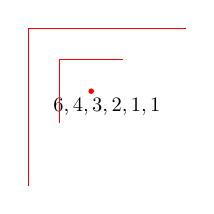
\begin{tikzpicture}
\node[scale=0.74] at (0,0) {$\ydiagram{6,4,3,2,1,1}$};
\draw[red] (-1,-1) -- (-1,1) -- (1,1);
\draw[red] (-0.6,-0.2) -- (-0.6,0.6) -- (0.2,0.6);
\fill[red] (-0.2,0.2) circle (1pt);
\end{tikzpicture}}}\longleftrightarrow\vcenter{\hbox{\begin{tikzpicture}
\node[scale=0.74] at (0,0) {$\ydiagram{11,5,1}$};
\draw[red] (-2,0.4) -- (2,0.4);
\draw[red] (-2,0) -- (-0.4,0);
\fill[red] (-2,-0.4) circle (1pt);
\end{tikzpicture}}}$
\end{figure}
\end{proof}
\end{hl}
\end{proposition}

\begin{proposition}
For all $n\geq 2$, $p(n)-p(n-1)$ counts the number of partitions of $n$ in which the two largest parts are equal.

\begin{hl}
\begin{proof}
The number of partitions of $n$ in which the two largest parts are equal, call this $\tilde p(n)$, can be put in bijective correspondence via the transpose with partitions in $P([n])$ all of whose parts are greater than 1. Through negative counting, this equals $p(n)$ minus the number of partitions containing 1. The partitions containing 1 can be bijected to partitions of $n-1$ by removing a 1, so that $\tilde p(n)=p(n)-p(n-1)$.
\end{proof}
\end{hl}
\end{proposition}

\begin{proposition}
For all positive integers $n$, $p(1)+p(2)+\cdots+p(n)<p(2n)$.

\begin{hl}
\begin{proof}
We claim that the LHS counts $\lambda\vdash 2n$ such that $n\leq\lambda_1<2n$, so that clearly the inequality holds. Specifically, LHS conditions on $\lambda_1$, so that $p(1)$ counts the case when $\lambda_1=2n-1$, $p(2)$ counts the case when $\lambda_1=2n-2$, and more generally $p(k)$ counts the case when $\lambda_1=2n-k$. Indeed, any $\tilde\lambda\in P([k])$ will have $\tilde\lambda_1\leq k\leq n$, so that inserting a row of $2n-k\geq n$ at the top of the Young diagram for $\tilde\lambda$ yields a valid Young diagram for some $\lambda\in P([2n])$.
\end{proof}
\end{hl}
\end{proposition}

\begin{example}
The \emph{Durfee square} of a partition $\lambda\vdash n$ is the largest square fitting in the upper left corner of the Young diagram, such as in the following:
\begin{figure}[H]
\centering
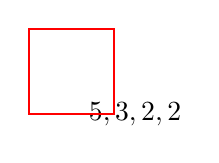
\begin{tikzpicture}
\node at (0,0) {$\ydiagram{5,3,2,2}$};
\draw[red,thick] (-1.35,0) rectangle (-0.27,1.08);
\end{tikzpicture}
\end{figure}

The width of this square can be computed without drawing the Young diagram. In particular, list $\lambda=(\lambda_1,\dots,\lambda_k)\vdash n$. Identify the largest $j$ such that $\lambda_j\geq j$. The width of the Durfee square will then be $j$.

\medskip

To prove this, note that the Durfee square has width $j$ iff the Young diagram contains square $(j,j)$ but not $(j+1,j+1)$, where we count from the top left. $(j,j)$ is in the Young diagram iff $\lambda_j\geq j$, and $(j+1,j+1)$ is not in the Young diagram iff $\lambda_{j+1}<j+1$. $\lambda$ is monotone decreasing, so that $\lambda_{j+1}<j+1$ implies $\lambda_{i}<i$ for all $i\geq j+1$. Hence, the width of the Durfee square can be identified by finding the largest $j$ such that $\lambda_j\geq j$.
\end{example}

\begin{example}
For all $k\leq n$, we have $p_k(n)\leq (n-k+1)^{k-1}$.
\begin{arrows}
\item In particular, this shows $p_k(n)$ cannot be a polynomial in $n$. If it were, it would have to be of degree at most $k-1$, but it would have $k$ zeros for $0\leq n\leq k-1$
\end{arrows}

\begin{hl}
\begin{proof}
Consider the Young diagram for some $\lambda\in P_k([n])$. The maximal width of the Young diagram is $n-k+1$, which occurs if all parts other than the first are 1. Further note that the last part is entirely determined by the previous $k-1$ parts, since they must sum to $n$. Hence, the number of Young diagrams is upper-bounded by $(n-k+1)^{k-1}$, where we pick each of the first $k-1$ rows to be between 1 and $n-k+1$ in length.
\end{proof}
\end{hl}
\end{example}

\begin{theorem}
The generating function for the number of integer partitions $p(n)$ is:
\begin{equation*}
\mathcal E(x)=\sum_{n=0}^\infty p(n)x^n=\frac1{1-x}\frac1{1-x^2}\cdots=\prod_{j=1}^\infty\frac1{1-x^j}
\end{equation*}
\begin{arrows}
\item Although this appears to be an infinite product, we note that only finitely many factors contribute to the coefficient for any $x^n$. Indeed, $\frac1{1-x^j}=1+x^j+x^{2j}+\cdots$, so that $\frac1{1-x^j}$ has no contribution when $j>n$.
\end{arrows}

\begin{hl}
\begin{proof}
This is an immediate application of counting using the products of generating functions. Note that an integer partition of $n$ can be represented as a tuple $(a_1,a_2,\dots,a_n)$. $a_j$ is a multiple of $j$, and represents the contribution of all $j$ terms in the integer partition. $\mathcal E(x)$ counts the number of ways to divide $n=1+\cdots+1$ into the different components of the tuple under this restriction, since $\frac1{1-x_j}=1+x^j+x^{2j}+\dots$.

\medskip

More formally, we note that the combinatorial class of integer partitions is isomorphic to $\operatorname{MSET}(\operatorname{SEQ}(\mathcal Z)\setminus\{\square\})$ where $\mathcal Z$ is the atomic class. Indeed, $\operatorname{SEQ}(\mathcal Z)\setminus\{\square\}$ is isomorphic to $\N$, so that taking the multiset yields (unordered) integer partitions. Now apply the rules for the generating functions.
\end{proof}
\end{hl}
\end{theorem}

\begin{theorem}[Hardy/Ramanujan]
$\displaystyle p(n)\sim\frac1{4n\sqrt3}e^{\pi\sqrt{2n/3}}$.
\begin{arrows}
\item $a_n\sim b_n$ means $\lim_{n\rightarrow\infty}\frac{a_n}{b_n}=1$.
\end{arrows}
\end{theorem}

\begin{example}
Let $f(n)$ count the number of partitions of $n$ such that no part is equal to 2. Let $F(x)=\sum_{n\geq0}f(n)x^n=\frac1{1-x}\cdot1\cdot\frac1{1-x^3}\cdot\cdots=(1-x^2)\mathcal E(x)$. Then for $n\geq 2$:
\begin{equation*}
f_n
=[x^n](1-x^2)\mathcal E(x)
=[x^n]\mathcal E(x)-[x^{n-2}]\mathcal E(x)
=p(n)-p(n-2)
\end{equation*}
\end{example}

\begin{proposition}
\;
\begin{enumerate}
\item $\displaystyle d(x)=\prod_{j=1}^\infty(1+x^j)$ is the generating function counting the number of integer partitions with distinct parts.
\item $\displaystyle o(x)=\prod_{j=0}^\infty\frac1{1-x^{2j+1}}$ is the generating function counting the number of integer partitions using only odd parts.
\item Let $p_d(n)$ be the number of ways to partition $n$ into distinct parts. Let $p_o(n)$ be the number of ways to partition $n$ into parts all of which are odd. Then $p_d(n)=p_o(n)$.
\end{enumerate}

\begin{hl}
\begin{proof}
The first two parts follow by counting with products of generating functions. Now perform the following manipulations, noting that even power of $j$ cancel:
\begin{equation*}
d(x)
=\prod_{j=1}^\infty(1+x^j)
=\prod_{j=1}^\infty\frac{1-x^{2j}}{1-x^j}
=\prod_{\substack{j=1\\j\text{ odd}}}^\infty\frac{1}{1-x^j}
=o(x)
\end{equation*}

We can also form a bijection. Beginning with a partition into distinct parts, iteratively replace each even number $2n$ with $n+n$ until all are odd. Beginning with a partition into odd parts, iteratively combine pairs of identical parts $n+n$ into $2n$. Since order is irrelevant in integer partitions, it is clear that both these procedures are order independent and terminate at a single possible partition. Furthermore, these procedures are inverses, making it a bijection.
\end{proof}
\end{hl}
\end{proposition}

\begin{proposition}
The number of partitions of $n$ with no parts equal to 1 or 2 is $p(n)-p(n-1)-p(n-2)+p(n-3)$.

\begin{hl}
\begin{proof}
The number of partitions with at least one part equal to 1 is $p(n-1)$; a bijection is formed by adding/removing a 1. Similarly, the number of partitions with at least one 2 is $p(n-2)$, and the number of partitions with both is $p(n-3)$. Now apply inclusion/exclusion.
\end{proof}
\end{hl}
\end{proposition}

\begin{theorem}
$\displaystyle np(n)=\sum_{k=1}^n\sigma(k)p(n-k)$, where $\sigma(n)$ is the sum of all divisors of $n$. For example, $\sigma(6)=1+2+3+6=12$.

\begin{hl}
\begin{proof}
We calculate $\mathcal E'(x)$ via logarithmic differentiation. In particular, $\log\mathcal E(x)=-\sum_{j=1}^\infty\log(1-x^j)$, so that taking the derivative yields:
\begin{equation*}
\frac{\mathcal E'(x)}{\mathcal E(x)}=\sum_{j=1}^\infty\frac{jx^{j-1}}{1-x^j}
\end{equation*}

Rearrange to obtain $x\mathcal E(x)=\mathcal E(x)\sum_{j=1}^\infty\frac{jx^j}{1-x^j}$. The LHS is the generating function for $np(n)$ by Wilf II, and by Wilf III, we have:
\begin{align*}
[x^n]\left(\mathcal E(x)\sum_{j=1}^\infty\frac{jx^j}{1-x^j}\right)
&=\sum_{k=0}^n\left([x^k]\sum_{j=0}^\infty\frac{jx^j}{1-x^j}\right)p(n-k)
=\sum_{k=0}^n\left([x^k]\sum_{j=1}^k\frac{jx^j}{1-x^j}\right)p(n-k)\\
&=\sum_{k=0}^n\left(\sum_{j=1}^k[x^{k-j}]\frac{j}{1-x^j}\right)p(n-k)
=\sum_{k=1}^n\left(\sum_{j=1}^kjI[j\mid k]\right)p(n-k)\\
&=\sum_{k=1}^n\sigma(k)p(n-k)\qedhere
\end{align*}
\end{proof}
\end{hl}
\end{theorem}

\subsection{Lah Numbers}

\begin{definition}
The \emph{unsigned Lah numbers} $\flbinom nk$ count the number of ways to partition $[n]$ into $k$ blocks, where a linear order is imposed within each block. The set of these structures is denoted $L([n],k)$. When considering all numbers of blocks, we denote the value by $\ell_n$, and the associated set $L([n])$.
\end{definition}

\begin{lemma}\label{exp_lah}
The exponential generating function for $\flbinom nk$ is $\displaystyle F_k(x)=\frac{(\frac x{1-x})^k}{k!}$, and the exponential generating function for $\ell_n$ is $F(x)=e^{\frac{x}{1-x}}$.

\begin{hl}
\begin{proof}
The exponential generating function for forming permutations is $\sum_{n=0}^\infty n!\frac{x^n}{n!}=\frac1{1-x}$. Thus, the exponential generating function for non-empty permutations is $\frac1{1-x}-1=\frac x{1-x}$. The second claim follows from forming the permutation structure on the corresponding labeled structure. For the first claim, use composition of exponential generating functions. We partition $L$ into blocks, form a nonempty permutation on each with exponential generating function $\frac x{1-x}$, and form a $k$-set from all the blocks with exponential generating function $x^k/k!$. Hence, we obtain $F_k(x)=(\frac x{1-x})^k/k!$.
\end{proof}
\end{hl}
\end{lemma}

\begin{proposition}\label{lah_closed}
$\displaystyle\flbinom nk=\binom{n-1}{k-1}\frac{n!}{k!}=\binom nk\frac{(n-1)!}{(k-1)!}$ for $n\geq k\geq1$.

\begin{hl}
\begin{proof}
Using Lemma \ref{exp_lah} and Theorem \ref{sum_bin_times_monom}:
\begin{align*}
\flbinom nk
&=n![x^n]\frac{(\frac x{1-x})^k}{k!}
=\frac{n!}{k!}[x^n]\frac{x^k}{(1-x)^{k+1}}(1-x)
=\frac{n!}{k!}\left([x^n]\frac{x^k}{(1-x)^{k+1}}-[x^{n-1}]\frac{x^k}{(1-x)^{k+1}}\right)\\
&=\frac{n!}{k!}\left(\binom nk-\binom{n-1}k\right)
=\frac{n!}{k!}\binom{n-1}{k-1}
\end{align*}

The second form then follows from Extraction/Absorption. We can also prove the second form combinatorially. Select the elements to start each block $\binom nk$ ways (this also ensures each block is nonempty). Sort the blocks so that the starting elements are in increasing order. We now must partition the remaining $n-k$ elements into $k$ blocks so that there is order within each partition, the partitions themselves are ordered, and any partition may be empty. This can be done with stars and bars: we order a set of $n-k$ elements and $k-1$ distinct bars $(n-1)!$ ways, then we remove the distinctness of the bars by diving by $(k-1)!$. Hence, $\flbinom nk=\binom nk\frac{(n-1)!}{(k-1)!}$.
\end{proof}
\end{hl}
\end{proposition}

\begin{proposition}\label{lah_to_stirling}
$\displaystyle\flbinom nk=\sum_{j=k}^n\sqbinom nj\setbinom jk$

\begin{hl}
\begin{proof}
Consider the summation. It counts how to partition $[n]$ into any number of cycles, and then form a set partition of the set of cycles into $k$ blocks. We can use labeled structures and the composition of exponential generating functions. The EGF for forming a permutation is $\log\frac1{1-x}$, and the EGF for forming set partitions into $k$ blocks is $\frac{(e^x-1)^k}{k!}$. Composing these yields:
\begin{equation*}
\sum_{n=0}^\infty\frac{x^n}{n!}\sum_{j=k}^n\sqbinom nj\setbinom jk
=\frac{(e^{\log(1/(1-x))}-1)^k}{k!}
=\frac{(\frac1{1-x}-1)^k}{k!}
=\frac{(\frac x{1-x})^k}{k!}
\end{equation*}

This is the EGF for $\flbinom nk$ by Lemma \ref{exp_lah}.

\medskip

Alternatively, we can use a combinatorial proof. LHS counts the number of ways to partition $[n]$ into $k$ nonempty blocks with internal linear order, and the RHS counts the number of ways to permute $[n]$, then distribute its cycles into $k$ nonempty blocks. The RHS can be equivalently carried out by partitioning $[n]$ into $k$ blocks and then forming a permutation within each block. So, it remains to show that we can biject a linear ordering to a permutation. But this is already clear via the one-line representation of permutations.
\end{proof}
\end{hl}
\end{proposition}

\begin{lemma}
$\displaystyle x^{\overline n}=\sum_{k=0}^n\flbinom nk(x)_k$ and $\displaystyle (x)_n=\sum_{k=0}^n\flbinom nk(-1)^{n-k}x^{\overline k}$

\begin{hl}
\begin{proof}
For the first claim, we use Proposition \ref{sqbinom_gen}, Theorem \ref{monomial_as_falling}, and Proposition \ref{lah_to_stirling} to write:
\begin{equation*}
x^{\overline n}
=\sum_{j=0}^n\sqbinom njx^j
=\sum_{j=0}^n\sqbinom nj\sum_{k=0}^j\setbinom jk(x)_k
=\sum_{k=0}^n(x)_k\sum_{j=k}^n\sqbinom nj\setbinom jk
=\sum_{k=0}^n\flbinom nk(x)_k
\end{equation*}

For the second claim, we use Corollary \ref{sqbinom_gen_alt}, Corollary \ref{monomial_as_rising}, and Proposition \ref{lah_to_stirling} to write:
\begin{align*}
(x)_n
&=\sum_{j=0}^n(-1)^{n-j}\sqbinom njx^j
=\sum_{j=0}^n(-1)^{n-j}\sqbinom nj\sum_{k=0}^j(-1)^{j-k}\setbinom jkx^{\overline k}
=\sum_{k=0}^n(-1)^{n-k}x^{\overline k}\sum_{j=k}^n\sqbinom nj\setbinom jk\\
&=\sum_{k=0}^n\flbinom nk(-1)^{n-k}x^{\overline k}\qedhere
\end{align*}
\end{proof}
\end{hl}
\end{lemma}


\section{Graphs}

\subsection{Chromatic Polynomials}

\begin{definition}
Let $G$ be a simple graph. An \emph{$n$-coloring} of $G$ is a map $c:V\rightarrow[n]$. It is a \emph{proper $n$-coloring} if adjacent vertices in $G$ has different colors, i.e., $c(u)\neq c(v)$ for all edges $uv$. The number of proper $n$-colorings is denoted $p_G(n)$, which is called the \emph{chromatic polynomial} of $G$.
\end{definition}

\begin{lemma}
Consider a graph $G$ with $d$ vertices. The chromatic polynomials for some common graphs include:
\begin{itemize}
\item If $|E|=0$, then $p(x)=x^d$
\item If $G$ is a tree, then $p(x)=x(x-1)^{d-1}$
\item If $G=K_d$ is a complete graph, then $p(x)=(x)_d$
\end{itemize}
\end{lemma}

\begin{theorem}[4-Color Theorem]
Every planar graph has a proper 4-coloring. Or, $p_G(4)>0$ for every planar graph.
\begin{arrows}
\item This was first introduced in 1852, but it was not proved until 1976. The proof relied on extensive computer computation and casework, and a simplified proof has been elusive.
\item The concept of a chromatic polynomial was introduced to help prove this. Despite it not yielding a proof, chromatic polynomials have received extensive research in combinatorics and graph theory.
\end{arrows}
\end{theorem}

\begin{definition}
Let $G=(V,E)$ be a graph with an edge $e=uv\in E$. Then the \emph{deletion operator} gives $G\setminus e=(V,E\setminus\{e\})$. The \emph{contraction operator} $G/e$ gives the graph obtained by identifying $u$ with $v$ (i.e., merging the two vertices via a quotient).
\end{definition}

\begin{lemma}\label{inductive_chrom}
For a simple graph $G=(V,E)$ and an edge $e\in E$, we have $p_G(n)=p_{G\setminus e}(n)-p_{G/e}(n)$.
\begin{arrows}
\item This provides a basis for proof by strong induction on $|E|$, since $G\setminus e$ has one fewer edge and $G/e$ has at least one fewer edge
\item It also provides a way to develop computational algorithms
\end{arrows}

\begin{hl}
\begin{proof}
Consider the proper $n$-colorings of $G\setminus e$. Each coloring either has $c(u)=c(v)$, in which case it is a coloring of $p_{G/e}$, or it has $c(u)\neq c(v)$, in which case it is a coloring of $G$. Each of these relationships are also bijective, so rearrange to obtain the result.
\end{proof}
\end{hl}
\end{lemma}

\begin{proposition}
If $G=(V,E)$ is a simple graph, then $p_G(n)$ is a polynomial of degree $|V|$ with integer coefficients.

\begin{hl}
\begin{proof}
This is proved by induction on $|E|$. The base case of $|E|=0$ gives $p_G(n)=n^{|V|}$, which satisfies the claim. By induction for $|E|>0$, using Lemma \ref{inductive_chrom}, we can write $p_G(n)$ as a difference of a $|V|$-degree and a $(|V|-1)$-degree polynomial each with integer coefficients. The result is that $p_G(n)$ has integer coefficients and degree $|V|$.
\end{proof}
\end{hl}
\end{proposition}

\begin{corollary}
Write the chromatic polynomial of $G$ as $p_G(n)=c_dn^d+c_{d-1}n^{d-1}+\cdots+c_0$. Then:
\begin{itemize}
\item $c_d=1$
\item $c_0=0$
\item $c_{d-1}=-|E|$
\item $(-1)^dp_G(-n)>0$ for all $n\geq 1$
\end{itemize}

\begin{hl}
\begin{proof}
This follows via induction on $|E|$ using Lemma \ref{inductive_chrom}. The base case holds for all the claims when $|E|=0$, since the chromatic polynomial is $n^d$ which has $c_d=1$, $c_0=0$, $c_{d-1}=0$, and $(-1)^d(-n)^d=n^d>0$. For $|E|>0$, by Lemma \ref{inductive_chrom}, $p_G(n)$ is the difference of a $|V|$-degree and a $(|V|-1)$-degree polynomial each with fewer edges. By induction, we thus have:
\begin{itemize}
\item The leading coefficient of $p_G(n)$ is the same as the leading coefficient of $p_{G\setminus e}(n)$, which is 1
\item The constant term of $p_G(n)$ is the difference of the constant terms of the two polynomials, each of which have constant term 0. Hence, $p_G(n)$ also has constant term zero
\item The term $c_{d-1}$ in $p_G(n)$ is the difference of the term $c_{d-1}$ in $p_{G\setminus e}(n)$ and the leading coefficient of $p_{G/e}(n)$. By induction, this is $-(|E|-1)-1=-|E|$
\item We have $(-1)^dp_G(n)=(-1)^d(p_{G\setminus e}(n)-p_{G/e}(n))=(-1)^dp_{G\setminus e}(n)+(-1)^{d-1}p_{G/e}(n)$, where each summand is positive by induction
\end{itemize}
\end{proof}
\end{hl}
\end{corollary}

\begin{theorem}\label{folklore}
Let $H$ and $L$ be graphs such that $H\cap L=K_d$. Let $G=H\cup L$. Then $p_G(x)=\frac{p_H(x)\cdot p_L(x)}{(x)_d}$.

\begin{hl}
\begin{proof}
The intersection $K_d$ contains $d$ distinct colors. Consider equivalence classes of colorings on $H$, $L$, and $G$ where two colorings are equivalent if the $d$ colors in $K_d$ are the same. By symmetry (namely, picking a permutation of the colors that switches the colors in $K_d$ to any other set), we have that all equivalence classes for a given graph are the same size. There are $(x)_d$ such equivalence classes, so that the size of each equivalence class is $p(x)/(x)_d$. Pick the equivalence class $(x)_d$ ways, pick the remaining coloring on $H$ $p_H(x)/(x)_d$ ways, and pick the remaining coloring on $L$ $p_L(x)/(x)_d$ ways. Multiply these together to obtain the form for $p_G(x)$.
\end{proof}
\end{hl}
\end{theorem}

\begin{example}
Consider the graph given below:
\begin{figure}[H]
\centering
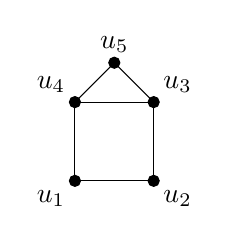
\begin{tikzpicture}
    \coordinate (A) at (0,0);
    \coordinate (B) at (1,0);
    \coordinate (C) at (1,1);
    \coordinate (D) at (0,1);
    \coordinate (E) at (0.5,1.5);

    \draw (A) -- (B) -- (C) -- (D) -- cycle;
    \draw (D) -- (E) -- (C);

    \foreach \vertex/\label/\position in {A/$u_1$/below left, B/$u_2$/below right, C/$u_3$/above right, D/$u_4$/above left, E/$u_5$/above}
    {
        \filldraw (\vertex) circle (2pt);
        \node at (\vertex) [\position] {\label};
    }
\end{tikzpicture}
\end{figure}

Let $H=\{u_1,u_2,u_3,u_4\}$ and $L=\{u_3,u_4,u_5\}$. Then they intersect on $\{u_3,u_4\}$, which is $K_2$. Using Lemma \ref{inductive_chrom}, we find that $p_H(x)=x(x-1)(x^2-3x+3)$, and we have that $p_L(x)=x(x-1)(x-2)$. Hence, Theorem \ref{folklore}, we have $p_G(x)=x(x-1)(x-2)(x^2-3x+3)$.
\end{example}

\begin{definition}
Let $G$ be a graph with vertices $V(G)=\{u_1,\dots,u_d\}$. We define an \emph{orientation} on $G$, denoted $\theta$, which specifies an order for each element in $E(G)$. The unordered pairs in $E(G)$ become ordered pairs in $\theta$, so that if $uv\in\theta$, then $u\rightarrow v$ in $G$.
\end{definition}

\begin{definition}
A \emph{directed path} in $G$ with orientation $\theta$ is a sequence of distinct vertices $x_{j-1}\rightarrow x_j$ for $j=1,\dots,s$ directed according to the given $\theta$. In addition, if $x_s\rightarrow x_0$, then $x_0\rightarrow x_1\rightarrow\cdots\rightarrow x_s\rightarrow x_0$ is called a \emph{directed cycle}.
\end{definition}

\begin{definition}
An orientation $\theta$ is called \emph{acyclic} if there are no directed cycles.
\end{definition}

\begin{definition}
For a proper $n$-coloring $c:V\rightarrow[n]$, the orientation induced by $c$ is $\theta=\{u_iu_j\in E\mid c(u_i)>c(u_j)\}$. In other words, all edges point from lower colors to higher colors.
\begin{arrows}
\item The induced orientation will clearly be acyclic.
\end{arrows}
\end{definition}

\begin{definition}
Consider $(\theta,c)$ where $\theta$ is an orientation and $c$ is an $n$-coloring, not necessarily proper. $(\theta,c)$ is called \emph{compatible} if for every oriented edge $u\rightarrow v$ we have $c(u)\leq c(v)$. It's called \emph{strictly compatible} if $c(u)<c(v)$.
\end{definition}

\begin{proposition}
If $(\theta,c)$ is strictly compatible, then $c$ is a proper $n$-coloring and $\theta$ is acyclic.

\begin{hl}
\begin{proof}
If $(\theta,c)$ is strictly compatible, then since each edge $uv$ is directed, we have either $c(u)>c(v)$ or $c(u)<c(v)$. In particular, $c(u)\neq c(v)$, so that the coloring is proper. To prove that $\theta$ is acyclic, suppose for contradiction there existed a directed cycle $u_{i_1}\rightarrow u_{i_2}\rightarrow\cdots\rightarrow u_{i_k}\rightarrow u_{i_1}$. Then $c(u_{i_1})<c(u_{i_2})<\cdots<c(u_{i_k})<c(u_{i_1})$, which yields a contradiction.
\end{proof}
\end{hl}
\end{proposition}

\begin{theorem}
Let $G$ be a finite simple graph, and consider its chromatic polynomial $p_G(x)$. Then $(-1)^{|V|}p_G(-n)$ equals the number of compatible pairs $(\theta,c)$, where $\theta$ is acyclic and $c$ is an $n$-coloring.

\begin{hl}
\begin{proof}
Let $\lambda_G(n)$ count the number of compatible pairs. We claim $\lambda_G(n)=\lambda_{G\setminus e}(n)+\lambda_{G/e}(n)$ for any fixed $e=uv$. Fix any compatible orientation $\theta$ and coloring $c$ on $G$, and consider the following cases regarding $e$:
\begin{itemize}
\item $c(u)\neq c(v)$. These pairs are in bijective correspondence with the pairs on $G\setminus e$ for which $c(u)\neq c(v)$, with the bijection formed by adding/removing $u\rightarrow v$ in the case $c(u)<c(v)$, or adding/removing $v\rightarrow u$ in the case $c(v)<c(u)$.
\item $c(u)=c(v)$, and switching the orientation of $uv$ yields a cyclic orientation. These pairs are in bijective correspondence with the pairs on $G\setminus e$ for which $c(u)\neq c(v)$ and there exists a directed path connecting $u$ and $v$ in some order. The inverse is uniquely defined since only one of $u\rightarrow v$ or $v\rightarrow u$ yields an acyclic orientation.
\item $c(u)=c(v)$, $u\rightarrow v$, and switching the orientation of $uv$ yields an acyclic orientation. These pairs are in bijective correspondence with the pairs on $G\setminus e$ for which $c(u)\neq c(v)$ and there do not exist any paths connecting $u$ and $v$.
\item $c(u)=c(v)$, $v\rightarrow u$, and switching the orientation of $uv$ yields an acyclic orientation. These pairs are in bijective correspondence with the pairs on $G/e$ via the natural bijection. The orientation on $G/e$ will be acyclic since $u\rightarrow v$ and $v\rightarrow u$ are acyclic.
\end{itemize}

Altogether, we have $\lambda_G(n)=\lambda_{G\setminus e}(n)+\lambda_{G/e}(n)$. Now we use this to prove our claim by induction on $|E|$. When $|E|=0$, there is one orientation with $n^{|V|}$ compatible colorings, so $\lambda_G(n)=n$. We have $p_G(x)=x^{|V|}$, hence $(-1)^{|V|}p_G(-n)=(-1)^{|V|}(-n)^{|V|}=n^{|V|}=\lambda_G(n)$. Now consider $|E|>0$:
\begin{align*}
\lambda_G(n)
&=\lambda_{G\setminus e}(n)+\lambda_{G/e}(n)
=(-1)^{|V|}p_{G\setminus e}(n)+(-1)^{|V|-1}p_{G/e}(n)\\
&=(-1)^{|V|}[p_{G\setminus e}(n)-p_{G/e}(n)]
=(-1)^{|V|}p_G(n)\qedhere
\end{align*}
\end{proof}
\end{hl}
\end{theorem}

\begin{example}
Consider a triangular graph. It is a complete graph, so that $p_G(x)=x(x-1)(x-2)$. Using $n=1$ gives the number of acyclic orientations, which is $(-1)^3p_G(-1)=6$. Substituting $n=2$ gives 24, which is the number of ways to color the graph with 2 colors and then create an acyclic compatible orientation.
\end{example}

\subsection{Trees}

\begin{definition}
A \emph{tree} is a simple, undirected, connected, acyclic graph.
\end{definition}

\begin{proposition}\label{tree_has_leaf}
Every tree contains at least two leaf nodes.

\begin{hl}
\begin{proof}
Suppose for contradiction a tree exists that violates this. Start at a leaf node (if exactly one exists) or an arbitrary node (if no leaf nodes exist). Move along an arbitrary edge, and remove that edge. Note that this prevents us from visiting the starting node if it was a leaf node. Since any nodes we visit in this manner cannot be leaf nodes, we will either always find another edge to traverse, or we will visit the same node multiple times. The former contradicts the fact that the tree has finitely many edges, while the latter contradicts the fact that the tree is acyclic.
\end{proof}
\end{hl}
\end{proposition}

\begin{lemma}
Every tree with $n$ vertices has $n-1$ edges.

\begin{hl}
\begin{proof}
When $n=1$, this is trivial. For higher $n$, we can find a leaf node by Proposition \ref{tree_has_leaf}. Both this leaf node and its outgoing edge can be removed to yield a valid tree with one fewer edge and one fewer node. Continue until the trivial case is reached.
\end{proof}
\end{hl}
\end{lemma}

\begin{lemma}\label{n_m_1_connected}
Any simple, undirected, acyclic graph with $n$ vertices and $n-1$ edges must be connected, and is thus a tree.

\begin{hl}
\begin{proof}
If it is not connected, then it can be represented as a union of several disconnected trees. Let the size of these trees be $n_i$, so that $\sum_{i=1}^kn_i=n$. The number of edges is thus $\sum_{i=1}^k(n_i-1)=n-k<n-1$, a contradiction.
\end{proof}
\end{hl}
\end{lemma}

\begin{lemma}\label{num_labeled_trees}
The number of \emph{labeled trees} (those with nodes labeled in $[n]$) is $n^{n-2}$, or $0$ when $n=0$.

\begin{hl}
\begin{proof}
When $n=0$, we define the number of labeled trees to be 0. $n=1$ is trivial.

\medskip

Otherwise, we form a bijection from labeled trees to $[n]^{n-2}$. To convert a tree into a sequence, iteratively remove the leaf with the smallest label, and append to the sequence its unique neighbor. Repeat until two nodes remain, at which point the process is terminated.

\medskip

To invert this, first note that all labels not appearing in the sequence must be leaf nodes. Indeed, if they were internal nodes, one of their two neighbors would have to be removed in order to reach a tree with two nodes. Conversely, these are the only leaf nodes, since a label occurring in the sequence must have at least two neighbors in order for one to be removed.

\medskip

Consider the label set, which contains all eligible labels. Identify all eligible labels not present in the code. There will be at least two, since the label set is two larger in size than the sequence. Identify the smallest, and connect it to the first element in the code. Now remove the first element in the code and remove the smallest element from the label set. Now recursively apply this procedure until the code is empty, at which point the remaining two nodes are connected.

\medskip

In order to show that the inverse is well-defined on all of $[n]^{n-2}$, we must prove that the result is simple, connected, and acyclic. It cannot add the same edge twice, since each recursive step removes a node from consideration. It cannot add a loop, since a node cannot both be in the code and not in the code. For each edge added, one of its endpoints is permanently removed from the label set and thus cannot have additional edges added to it, so that the resulting graph is acyclic. The resulting acyclic graph has $n-1$ edges, so that it must be a tree by Lemma \ref{n_m_1_connected}.

\medskip

We have an inverse for our forward map on the image of that map, but it remains to show the forward map is surjective or that the inverse is injective on its entire domain. We prove the latter. Suppose two sequences produces the same tree. The leaf nodes of that tree are determined by the elements not in the sequence, so that both sequences must use the same subset of $[n]$. The lowest leaf node is always connected solely to the first element in the sequence, so that both codes must have the same first element. Now, recursively, continue this argument by looking at the subtree without this node.
\end{proof}
\end{hl}
\end{lemma}

\begin{definition}
A \emph{plane tree} is a rooted tree in which an ordering is specified for the children of each vertex.
\end{definition}

\begin{definition}
A \emph{$k$-ary tree} is a plane tree such that the number of children of any node is either $0$ and $k$. Let $\mathcal T^{\{0,k\}}$ denote the class of $k$-ary trees. The \emph{size} of a $k$-ary tree is defined as its number of nodes.
\end{definition}

\begin{definition}
For $\Omega\subset\W$ and $0\in\Omega$, let $\mathcal T^{\Omega}$ be the class of plane trees such that the number of children at each node lies in $\Omega$. These trees are called \emph{$\Omega$-restricted trees}. The \emph{characteristic function} encapsulating $\Omega$ is $\phi(z)=\sum_{k\in\Omega}z^k$.
\begin{arrows}
\item As an example, the class of $k$-ary trees has characteristic $\phi(z)=1+z^k$ and the class of unrestricted plane trees has characteristic $\phi(z)=(1-z)^{-1}$.
\end{arrows}
\end{definition}

\begin{proposition}
The ordinary generating function $T^{\Omega}(x)$ for $\Omega$-restricted trees satisfies the functional equation $T^\Omega(x)=x\phi(T^{\Omega}(x))$. Therefore, by Lagrange Inversion:
\begin{equation*}
[x^n]T^{\Omega}(x)
=\frac1n[z^{n-1}]\phi(z)^n
\end{equation*}

\begin{hl}
\begin{proof}
This follows from using combinatorial classes. $\mathcal T^{\Omega}=\mathcal Z\times\operatorname{SEQ}_{\Omega}(\mathcal T^{\Omega})$, so that $T^{\Omega}(x)=x\sum_{k\in\Omega}T^{\Omega}(x)^k=x\phi(T^{\Omega}(x))$.
\end{proof}
\end{hl}
\end{proposition}

\begin{example}
The number of size-$n$ trees in $\mathcal T^{\{0,1,3\}}$ is $\displaystyle\frac1n\sum_{\substack{k=1\\k\text{ odd}}}^n\binom nk\binom{n-k}{(k-1)/2}$.

\begin{hl}
\begin{proof}
\begin{align*}
[x^n]T(x)
&=\frac1n[z^{n-1}](1+z+z^3)^n
=\frac1n[z^{n-1}]\sum_{k=0}^n\binom nk(z+z^3)^{n-k}\\
&=\frac1n\sum_{k=0}^n\binom nk[z^{n-1}]z^{n-k}(1+z^2)^{n-k}
=\frac1n\sum_{k=1}^n\binom nk[z^{k-1}](1+z^2)^{n-k}\\
&=\frac1n\sum_{\substack{k=1\\k\text{ odd}}}^n\binom nk[z^{(k-1)/2}](1+z)^{n-k}
=\frac1n\sum_{\substack{k=1\\k\text{ odd}}}^n\binom nk\binom{n-k}{(k-1)/2}
\end{align*}

In the first binomial expansion, we used the power $n-k$ instead of $k$ to cancel out the $n$ in $[z^{n-1}]$. If we used $k$ instead, we would have $[z^{n-k-1}](1+z^2)^k$, which is harder to deal with since now the parity of $k$ for which this is nonzero depends also on the parity of $n$.
\end{proof}
\end{hl}
\end{example}

\begin{example}
The number of size-$n$ trees in $\mathcal T^{\{0,2,3\}}$ is $\displaystyle\frac1n\sum_{k=0}^n\binom nk\binom k{n-2k-1}$.

\begin{hl}
\begin{proof}
\begin{align*}
[x^n]T(x)
&=\frac1n[z^{n-1}](1+z^2+z^3)^n
=\frac1n\sum_{k=0}^n\binom nk[z^{n-1}](z^2+z^3)^k\\
&=\frac1n\sum_{k=0}^n\binom nk[z^{n-2k-1}](1+z)^k
=\frac 1n\sum_{k=0}^n\binom nk\binom k{n-2k-1}\qedhere
\end{align*}
\end{proof}
\end{hl}
\end{example}

\begin{example}
Suppose we change the size of a tree in $\mathcal T^{\{0,2,3\}}$ to be the number of non-leaf nodes. Denote this class by $\overline{\mathcal T}$. The number of trees of size $n=1$ is $1$, and when $n>1$, the number of trees of size $n$ is $\displaystyle\frac1n\sum_{k=0}^{n-1}\binom{2n}k\binom n{n-k-1}2^{k+1}$.

\begin{hl}
\begin{proof}
Any tree in $\overline{\mathcal T}$ is either a lone root or a root with 2 or 3 children. Then $\overline{\mathcal T}=\{\square\}+\mathcal Z\times\operatorname{SEQ}_{\{2,3\}}(\overline{\mathcal T})$. This yields $\overline T(x)=1+x(\overline T(x)^2+\overline T(x)^3)$. Let $z(x)=\overline T(x)-1$ and $\phi(z)=(z+1)^2(z+2)$. Then $z(x)=x(\overline T(x)^2+\overline T(x)^3)=x((z+1)^2+(z+1)^3)=x(z+1)^2(z+2)=x\phi(z)$. Apply Lagrange Inversion for $n\geq1$ to obtain:
\begin{align*}
[x^n]z(x)
&=\frac1n[z^{n-1}]\phi(z)^n
=\frac1n[z^{n-1}](z+1)^{2n}(z+2)^n
=\frac1n\sum_{k=0}^{n-1}[z^k](z+1)^{2n}\cdot[z^{n-k-1}](z+2)^n\\
&=\frac 1n\sum_{k=0}^{n-1}\binom{2n}k\binom n{n-k-1}2^{k+1}\qedhere
\end{align*}
\end{proof}
\end{hl}
\end{example}

\section{Generating Functions}

\subsection{Definitions}

\begin{definition}
A \emph{formal power series} is a summation $\sum_{n=0}^\infty a_nx^n$ for a sequence of coefficients $\{a_n\}$
\begin{arrows}
\item Two series are equal if the coefficients are equal
\item The formal power series corresponding to $\{a_n\}$ is called its \emph{ordinary generating function}, and the relationship is denoted $\sum_{n=0}^\infty a_nx^n\ogf \{a_n\}$
\end{arrows}
\end{definition}

\begin{proposition}
Let $\F[[x]]$ denote the space of formal power series over a field $\F$, such as $\C[[x]]$. This forms an algebra with the operations:
\begin{enumerate}[label=(\roman*)]
\item Addition: $\displaystyle\sum_{n=0}^\infty a_nx^n+\sum_{n=0}^\infty b_nx^n=\sum_{n=0}^\infty(a_n+b_n)x^n$
\item Scalar Multiplication: $\displaystyle c\sum_{n=0}^\infty a_nx^n=\sum_{n=0}^\infty ca_nx^n$
\item Multiplication: $\displaystyle\left(\sum_{n=0}^\infty a_nx^n\right)\left(\sum_{n=0}b_nx^n\right)=\sum_{n=0}^\infty\left(\sum_{k=0}^na_kb_{n-k}\right)x^n$
\end{enumerate}
\end{proposition}

\begin{definition}
$[x^k]:\F[[x]]\rightarrow\F$ defined by $[x^k]\sum_{n=0}^\infty a_nx^n=a_k$ is a linear functional. In $\F[[x]]$, we have $[x^k]\sum_{n=0}^\infty a_nx^n=0$ for all $k<0$.
\end{definition}

\begin{proposition}
$[x^n]$ satisfies the following properties:
\begin{itemize}
\item Linearity: $\displaystyle [x^n](\alpha A(x)+\beta B(x))=\alpha[x^n]A(x)+\beta[x^n]B(x)$
\item Shifting: $\displaystyle [x^n]x^kA(x)=[x^{n-k}]A(x)$ for $n\geq k$
\item Differentiation: $\displaystyle [x^n]A'(x)=(n+1)[x^{n+1}]A(x)$ (using formal differentiation in Proposition \ref{formal_differentiation})
\item Convolution: $\displaystyle [x^n]A(x)B(x)=\sum_{k=0}^n([x^k]A(x))([x^{n-k}]B(x))$
\item Composition: $\displaystyle [x^n]A(B(x))=\sum_{k=0}^\infty [x^k]A(x)\cdot[x^n](B(x))^k$ (assuming this is well-defined in Definition \ref{formal_compose})

\begin{hl}
\begin{proof}
Linearity follows trivially, since $[x^n]$ is a linear functional. Shifting follows by definition of multiplication, and differentiation by definition in Proposition \ref{formal_differentiation}. Convolution follows by definition of multiplication. Composition is proved as follows (where the infinite sum is finite for any given $n$, so that linearity holds):
\begin{equation*}
[x^n]A(B(x))
=[x^n]\sum_{k=0}^\infty a_k(B(x))^k
=\sum_{k=0}^\infty a_k[x^n](B(x))^k
=\sum_{k=0}^\infty [x^k]A(x)\cdot[x^n](B(x))^k\qedhere
\end{equation*}
\end{proof}
\end{hl}
\end{itemize}
\end{proposition}

\begin{definition}
$G$ is a map from sequences in $\F$ to formal power series, so that $G(\{f_n\})=\sum_{n=0}^\infty f_nx^n$. For simplicity, we often denote $G(f_n)=G(\{f_n\})$.
\end{definition}

\begin{proposition}
$G$ satisfies the following properties:
\begin{itemize}
\item Linearity: $\displaystyle G(\alpha a_n+\beta b_n)=\alpha G(a_n)+\beta G(b_n)$
\item Shifting: $\displaystyle G(a_{n+1})=\frac{G(a_n)-a_0}x$
\item Differentiation: $\displaystyle G(na_n)=xD_xG(a_n)$
\item Convolution: $\displaystyle G\left(\sum_{k=0}^na_kb_{n-k}\right)=G(a_n)G(b_n)$
\item Composition: $\displaystyle \sum_{k=0}^\infty a_kG(b_n)^k=G(a_n)\circ G(b_n)$ (assuming this is well-defined in Definition \ref{formal_compose})
\end{itemize}

\begin{hl}
\begin{proof}
Linearity holds by the definition of addition for formal power series. Shifting follows trivially. Differentiation holds as follows:
\begin{equation*}
G(na_n)
=\sum_{n=0}^\infty na_nx^n
=x\sum_{n=0}^\infty na_nx^n{n-1}
=xD_xG(a_n)
\end{equation*}

Convolution holds by the definition of multiplication, and composition trivially holds.
\end{proof}
\end{hl}

\end{proposition}

\begin{theorem}\label{formal_reciprocal}
A formal power series has a reciprocal iff $a_0\neq0$, and it is unique if it exists.

\begin{hl}
\begin{proof}
Uniqueness follows from algebra (uniqueness of multiplicative inverses). For $\sum_{n=0}^\infty a_nx^n$, suppose $\left[\sum_{n=0}^\infty a_nx^n\right]\left[\sum_{n=0}^\infty b_nx^n\right]=1$. For $n=0$, this implies $a_0b_0=1$, so $a_0\neq0$ and $b_0=-a_0^{-1}$. For $n=1$, we have $a_0b_1+a_1b_0=0$, so $b_1=-a_0^{-1}a_1b_0$. This can be continued recursively to obtain a reciprocal.
\end{proof}
\end{hl}
\end{theorem}

\begin{definition}\label{formal_compose}
The composition of two formal power series $f(x)=\sum_{n=0}^\infty a_nx^n$ and $g(x)$ is $f(g(x))=\sum_{n=0}^\infty a_n g(x)^n$. However, this may not be well-defined. If $[x^0]g(x)\neq0$, then infinitely many terms in the above definition are needed to calculate each coefficient of the resulting power series, so since infinite series are not defined, neither is the power series. However, if $[x^0]g(x)=0$, then $a_n(g(x))^n=a_n(g_1x+g_2x^2+\cdots)^n=a_nx^n(g_1+g_2x+\cdots)$, so that finitely many terms are needed to compute each coefficient. So, the composition is well-defined if $[x^0]g(x)=0$ or if $f$ is a polynomial.
\end{definition}

\begin{proposition}\label{compose_inverse}
Suppose $[x^0]f(x)=0$. Then $f$ has an inverse $g$, so that $f(g(x))=x=g(f(x))$, iff $[x^1]f(x)\neq0$.
\end{proposition}

\begin{definition}
Let $\{f_k(x)\}_{k\geq0}$ be a sequence of formal power series. $f_k(x)$ converges to $f(x)$ if $[x^n]f_k(x)$ is eventually constant and equal to $[x^n]f(x)$ as $k\rightarrow\infty$ for all $n$.
\begin{arrows}
\item We require each $[x^n]f_k(x)$ to become constant since there is not necessarily a notion of convergence in the field $\F$
\end{arrows}
\end{definition}

\begin{example}
For a power series $A(x)=\sum_{n=0}^\infty a_nx^n$, the sequence of partial sums $s_k(x)=\sum_{n=0}^ka_nx^n$ converges to $A(x)$.
\end{example}

\begin{proposition}\label{formal_degree}
Define the \emph{degree} of a formal power series $f(x)$ to be the smallest $n$ such that $a_n\neq0$, denoted $\deg(f(x))$. If $f(x)=0$, then let $\deg(f(x))=\infty$. $\sum_{k=0}^\infty f_k(x)$ exists iff $\lim_{k\rightarrow\infty}\deg(f_k(x))\rightarrow\infty$.
\end{proposition}

\begin{proposition}\label{formal_differentiation}
Define \emph{differentiation} as $f'(x)=\sum_{n=0}^\infty na_nx^{n-1}$ for $f(x)=\sum_{n=0}^\infty a_nx^n$. All normal derivative rules such as the sum, product, and quotient rule hold for formal power series.
\end{proposition}

\begin{definition}
Other types of generating functions are also possible, such as:
\begin{table}[H]
\centering
\begin{NiceTabular}{llll}\toprule
Type&Abbreviation&Form&Notation\\\midrule
Ordinary Generating Function&ogf&$f(x)=\sum_{n=0}^\infty a_nx^n$&$f(x)\ogf \{a_n\}$\\
Exponential Generating Function&egf&$g(x)=\sum_{n=0}^\infty b_n\frac{x^n}{n!}$&$g(x)\overset{\text{egf}}{\longleftrightarrow}\{b_n\}$\\
Dirichlet Generating Function&dgf&$h(s)=\sum_{n=1}^\infty\frac{c_n}{n^s}$&$h(s)\overset{\text{dgf}}{\longleftrightarrow}\{c_n\}$\\\bottomrule
\end{NiceTabular}
\end{table}
\end{definition}

\subsection{Common Generating Functions}

\begin{example}\label{recip_1_minus_x}
$\displaystyle\frac1{1-x}=\sum_{n=0}^\infty x^n$, so that $\displaystyle[x^k]\frac1{1-x}=1$

\begin{hl}
\begin{proof}
This can be shown with the Generalized Binomial Theorem:
\begin{equation*}
(1-x)^{-1}=\sum_{n=0}^\infty\binom{-1}n(-x)^n=\sum_{n=0}^\infty\frac{(-1)_n}{n!}(-x)^n=\sum_{n=0}^\infty x^n
\end{equation*}

Or, carry out the multiplication:
\begin{equation*}
(1-x)\sum_{n=0}^\infty x^n=\sum_{n=0}^\infty x^n-\sum_{n=0}^\infty x^{n+1}=x^0=1\qedhere
\end{equation*}
\end{proof}
\end{hl}
\end{example}

\begin{lemma}\label{generating_func_recip_linear}
$\displaystyle[x^n]\frac1{1-ax}=a^n$

\begin{hl}
\begin{proof}
Substitute $ax$ for $x$ in Example \ref{recip_1_minus_x}.
\end{proof}
\end{hl}
\end{lemma}

\begin{lemma}\label{easier_gen_linear}
$\displaystyle[x^n]\frac1{x-a}=-\frac1{a^{n+1}}$

\begin{hl}
\begin{proof}
Using Lemma \ref{generating_func_recip_linear}, $\displaystyle [x^n]\frac1{x-a}=-\frac1a[x^n]\frac1{1-\frac1ax}=-\frac1{a^{n+1}}$.
\end{proof}
\end{hl}
\end{lemma}

\begin{lemma}\label{part_sums_gen}
$\displaystyle[x^n]\frac{A(x)}{1-x}=\sum_{k=0}^na_k$ from Example \ref{recip_1_minus_x} and definition of multiplication
\begin{arrows}
\item In other words, dividing by $1-x$ gives the partial sums
\end{arrows}
\end{lemma}
%
%\begin{example}
%$\displaystyle[x^n]\frac x{(1-x)^2}=n$
%
%\begin{hl}
%\begin{proof}
%\begin{equation*}
%\frac x{(1-x)^2}
%=x\frac d{dx}\frac1{1-x}
%=x\frac d{dx}\sum_{n=0}^\infty x^n
%=x\sum_{n=0}^\infty nx^{n-1}
%=\sum_{n=0}^\infty nx^n\qedhere
%\end{equation*}
%\end{proof}
%\end{hl}
%\end{example}

\begin{lemma}\label{binom_gen}
$\displaystyle[x^n]\frac{x^k}{(1-x)^{k+1}}=\binom nk$ by Theorem \ref{sum_bin_times_monom}.
\end{lemma}

\begin{lemma}\label{recip_power_subtract}
$\displaystyle [x^n]\frac1{(x-a)^k}=(-1)^k\left(\frac1a\right)^{n+k}\binom{n+k-1}{k-1}$

\begin{hl}
\begin{proof}
\begin{align*}
[x^n]\frac1{(x-a)^k}
&=[x^{n+k-1}]\frac{x^{k-1}}{(x-a)^k}
=\frac1a[x^{n+k-1}]\frac{(x/a)^{k-1}}{(x/a-1)^k}
=(-1)^k\frac1a[x^{n+k-1}]\frac{(x/a)^{k-1}}{(1-x/a)^k}\\
&\overset{\ref{binom_gen}}=(-1)^k\frac1a\cdot\left(\frac1a\right)^{n+k-1}\binom{n+k-1}{k-1}
=(-1)^k\left(\frac1a\right)^{n+k}\binom{n+k-1}{k-1}\qedhere
\end{align*}
\end{proof}
\end{hl}
\end{lemma}

%\begin{example}
%$\displaystyle[x^n]\frac{2x}{(1-x)^8}=2[x^{n+6}]\frac{x^7}{(1-x)^8}=2\binom{n+6}7$
%\end{example}

\begin{theorem}\label{central_gen}
$\displaystyle\sum_{n=0}^\infty\binom{2n}nx^n=\frac1{\sqrt{1-4x}}$ is the generating function for the central binomial coefficients.

\begin{hl}
\begin{proof}
This can be solved using the Generalized Binomial Theorem:
\begin{align*}
\frac1{\sqrt{1-4x}}
&=\sum_{n=0}^\infty\binom{-1/2}{n!}(-4x)^n
=1+\sum_{n=1}^\infty\frac{(-1/2)_n}{n!}(-4x)^n\\
&=1+\sum_{n=1}^\infty\frac{(-1)^n(2n-1)!!}{2^nn!}(-4x)^n
=1+\sum_{n=1}^\infty\frac{2^n(2n-1)!!}{n!}x^n
=1+\sum_{n=1}^\infty\frac{2^nn!(2n-1)!!}{n!n!}x^n\\
&=1+\sum_{n=1}^\infty\frac{(2n)!!(2n-1)!!}{n!n!}x^n
=1+\sum_{n=1}^\infty\frac{(2n)!}{n!n!}x^n
=1+\sum_{n=1}^\infty\binom{2n}nx^n
\end{align*}

Alternatively, we can use Lagrange Inversion. Note that $\binom{2n}n=[z^n](1+z)^{2n}$. We can thus use Theorem \ref{power_lif} with $W(z)=1$ and $\phi(z)=(1+z)^2$. To find $z$, we solve $z=x\phi(z)=x(1+z)^2$. We obtain $xz^2+(2x-1)z+x=0$, so that using the quadratic formula and picking the root which is well-defined at $x=0$ gives $z=\frac{-2x+1-\sqrt{1-4x}}{2x}$. Using this:

\begin{align*}
\sum_{n=0}^\infty\binom{2n}nx^n
&=\sum_{n=0}^\infty x^n[z^n](1+z)^{2n}
=\frac{1}{1-x\phi'(z)}
=\frac1{1-x\cdot 2(z+1)}
=\frac1{1-x\cdot 2(\frac{-2x+1-\sqrt{1-4x}}{2x}+1)}\\
&=\frac1{1-x\cdot 2(\frac{1-\sqrt{1-4x}}{2x})}
=\frac1{\sqrt{1-4x}}\qedhere
\end{align*}
\end{proof}
\end{hl}
\end{theorem}

\begin{theorem}\label{central_shifted_gen}
$\displaystyle\sum_{n=0}^\infty\binom{2n+k}nx^n=\frac1{\sqrt{1-4x}}\left(\frac{1-\sqrt{1-4x}}{2x}\right)^k$

\begin{hl}
\begin{proof}
This is a more general version of Theorem \ref{central_gen}, but it can be proved similarly. Note that $\binom{2n+k}n=[z^n](1+z)^{2n+k}$. We can thus use Theorem \ref{power_lif} with $W(z)=(1+z)^k$ and $\phi(z)=(1+z)^2$. From before, we have $z=\frac{-2x+1-\sqrt{1-4x}}{2x}$. Using this:

\begin{align*}
\sum_{n=0}^\infty\binom{2n+k}nx^n
&=\sum_{n=0}^\infty x^n[z^n](1+z)^{2n+k}
=\sum_{n=0}^\infty x^n[z^n](1+z)^k(1+z)^{2n}\\
&=\frac{(1+z)^k}{1-x\phi'(z)}
=\frac{(1+z)^k}{1-x\cdot 2(z+1)}
=\frac{(1+\frac{-2x+1-\sqrt{1-4x}}{2x})^k}{1-x\cdot 2(\frac{-2x+1-\sqrt{1-4x}}{2x}+1)}\\
&=\frac{(\frac{1-\sqrt{1-4x}}{2x})^k}{1-x\cdot 2(\frac{1-\sqrt{1-4x}}{2x})}
=\frac{1}{\sqrt{1-4x}}\left(\frac{1-\sqrt{1-4x}}{2x}\right)^k\qedhere
\end{align*}
\end{proof}
\end{hl}
\end{theorem}

\begin{theorem}
$\displaystyle\sum_{n=0}^\infty\frac{k(2n+k-1)!}{n!(n+k)!}x^n=\left(\frac{1-\sqrt{1-4x}}{2x}\right)^k$

\begin{hl}
\begin{proof}
We use Theorem \ref{central_shifted_gen}. We calculate:
\begin{align*}
A(x)
&=\sum_{n=0}^\infty\frac{k(2n+k-1)!}{n!(n+k)!}x^n
=1+\sum_{n=1}^\infty\frac kn\binom{2n+k-1}{n-1}x^n
=1+\sum_{n=1}^\infty\frac kn\binom{2(n-1)+k+1}{n-1}x^n
\end{align*}

Taking the derivative, we have:
\begin{align*}
A'(x)
&=k\sum_{n=1}^\infty\binom{2(n-1)+k+1}{n-1}x^{n-1}
=k\sum_{n=0}^\infty\binom{2n+k+1}{n}x^{n}
=\frac k{\sqrt{1-4x}}\left(\frac{1-\sqrt{1-4x}}{2x}\right)^{k+1}\\
&=\frac k{\sqrt{1-4x}}\left(\frac{1-\sqrt{1-4x}}{2x}\right)^{k-1}\frac{2-4x-2\sqrt{1-4x}}{4x^2}
\end{align*}

Letting $u=\frac{1-\sqrt{1-4x}}{2x}$, we have $\frac{du}{dx}=\frac{4x/\sqrt{1-4x}-2+2\sqrt{1-4x}}{4x^2}=\frac{2-4x-2\sqrt{1-4x}}{4x^2\sqrt{1-4x}}$. Hence, $A'(x)=k(u)^{k-1}\frac{du}{dx}$. Therefore, $A(x)=u^k$, giving us the claim.
\end{proof}
\end{hl}
\end{theorem}

%\begin{theorem} Commented because no citations and already in proof
%Let $a_n=\sum_{k=0}^n\binom nkb_k$, so that by Binomial Inversion, $b_n=\sum_{k=0}^n\binom nka_k(-1)^{n-k}$. Let $A(x),B(x)$ be the corresponding power series. Then:
%\begin{equation*}
%A(x)=\frac1{1-x}B\left(\frac x{1-x}\right)\quad\text{ and }\quad B(x)=\frac1{1+x}A\left(\frac x{1+x}\right)
%\end{equation*}
%
%\begin{hl}
%\begin{proof}
%Using Theorem \ref{sum_bin_times_monom}:
%\begin{multline*}
%A(x)
%=\sum_{n=0}^\infty a_nx^n
%=\sum_{n=0}^\infty\sum_{k=0}^n\binom nkb_kx^n
%=\sum_{k=0}^\infty b_k\sum_{n=k}^\infty\binom nkx^n\\
%=\sum_{k=0}^\infty b_k\frac{x^k}{(1-x)^{k+1}}
%=\frac1{1-x}\sum_{k=0}^\infty b_k\left(\frac{x}{1-x}\right)^k
%=\frac1{1-x}B\left(\frac{x}{1-x}\right)
%\end{multline*}
%
%Let $\widetilde a_n=(-1)^na_n$ and $\widetilde b_n=(-1)^nb_n$. By the above result, $\widetilde B(x)=\frac1{1-x}\widetilde A\left(\frac x{1-x}\right)$, or $B(-x)=\frac1{1-x}A\left(\frac x{x-1}\right)$. Replace $x$ with $-x$ to obtain $B(x)=\frac1{1+x}A\left(\frac{x}{1+x}\right)$.
%\end{proof}
%\end{hl}
%\end{theorem}

\subsection{Wilf Rules}

\begin{theorem}[Wilf Rules for OGFs]\label{wilf}
\;
\begin{enumerate}[label=\Roman*.]
\item\label{wilf1} If $F(x)\ogf \{f_n\}$, then for $k\geq0$, $\displaystyle\{f_{n+k}\}\ogf \frac{F(x)-f_0-f_1x-\cdots-f_{k-1}x^{k-1}}{x^k}$
\item\label{wilf2} If $F(x)\ogf \{f_n\}$ and $P$ is a polynomial, then $\{P(n)f_n\}\ogf  P(xD)F(x)$, where $D$ is the derivative operator with respect to $x$
\begin{arrows}
\item For example, $(xD)^2F(x)=x\frac d{dx}\left[x\frac d{dx}F(x)\right]$
\end{arrows}
\item\label{wilf3} If $F(x)\ogf \{f_n\}$ and $G(x)\ogf \{g_n\}$, then $\displaystyle F(x)G(x)\ogf \left\{\sum_{k=0}^na_kb_{n-k}\right\}$
\item\label{wilf4} If $F(x)\ogf\{f_n\}$ and $k\in\N$, then $\displaystyle F^k(x)\ogf\left\{\sum_{n_1+\cdots+n_k=n}a_{n_1}\cdots a_{n_k}\right\}$
\item\label{wilf5} If $F(x)\ogf\{f_n\}$, then $\displaystyle\frac1{1-x}F(x)\ogf\left\{\sum_{k=0}^nf_k\right\}$, i.e., $\displaystyle\frac1{1-x}F(x)$ is the generating function for the partial sums
\item\label{wilf6} If $F(x)\ogf\{f_n\}$, then $x^kF(x)\ogf\{a_{n-k}\}$, where $a_{n-k}=0$ when $n-k<0$
\end{enumerate}
\end{theorem}

\begin{example}
Suppose $a_{n+2}=3a_{n+1}-a_n$ with $a_0=1$ and $a_1=-3$. Then by Wilf I, $\frac{A(x)-a_0-a_1x^1}{x^2}=-3\frac{A(x)-a_0}x-A(x)$. Rearrange to obtain $A(x)-1+3x=-3xA(x)+3x-A(x)x^2$, or $A(x)=\frac1{1+3x+x^2}$.
\end{example}

\begin{example}
Suppose $a_n=n^2$, as in Example \ref{nsqgen}. Then by Wilf II and Lemma \ref{generating_func_recip_linear}:
\begin{equation*}
A(x)
=(xD)^2\frac1{1-x}
=x\frac{d}{dx}\left[x\frac d{dx}\frac1{1-x}\right]
=x\frac{d}{dx}\frac x{(1-x)^2}
=\frac{x(1+x)}{(1-x)^3}
\end{equation*}
\end{example}

\begin{theorem}[Wilf Rules for EGFs]\label{wilf_egf}
\;
\begin{enumerate}[label=\Roman*.]
\item If $F(x)\egf \{f_n\}$, then for $k\geq0$, $\displaystyle\{f_{n+k}\}\egf D^kF(x)$
\begin{arrows}
\item Shifting in the other direction is harder. Generally, just rewrite the recurrence so that it is a shift in the direction above (e.g., $a_{n+2}=a_{n+1}+2a_n$ rather than $a_{n}=a_{n-1}+2a_{n-2}$)
\end{arrows}
\item If $F(x)\egf \{f_n\}$ and $P$ is a polynomial, then $\{P(n)f_n\}\egf  P(xD)F(x)$, where $D$ is the derivative operator with respect to $x$
\begin{arrows}
\item This is the same as for OGFs
\end{arrows}
\item If $F(x)\egf \{f_n\}$ and $G(x)\egf \{g_n\}$, then $\displaystyle F(x)G(x)\egf \left\{\sum_{k=0}^n\binom nkf_kg_{n-k}\right\}$
\end{enumerate}

\begin{hl}
\begin{proof}
We prove Wilf III using the corresponding rule for ordinary generating functions:
\begin{equation*}
F(x)G(x)
=\left(\sum_{n=0}^\infty\frac{f_n}{n!}x^n\right)\left(\sum_{n=0}^\infty\frac{g_n}{n!}x^n\right)
\overset{\text{III}}=\sum_{n=0}^\infty\left(\sum_{k=0}^n\frac{f_kg_{n-k}}{k!(n-k)!}\right)x^n
=\sum_{n=0}^\infty\left(\sum_{k=0}^n\binom nkf_kg_{n-k}\right)\frac{x^n}{n!}
\end{equation*}
% todo finish proof for other rules
\end{proof}
\end{hl}
\end{theorem}

\begin{theorem}[Wilf Rules for DGFs]
\;
\begin{enumerate}[label=\Roman*.]
\item If $F(s)\overset{\text{dgf}}{\longleftrightarrow}\{f_n\}$ and $G(s)\overset{\text{dgf}}{\longleftrightarrow}\{g_n\}$, then $\displaystyle F(s)G(s)\overset{\text{dgf}}{\longleftrightarrow} \left\{\sum_{jk=n}^nf_jg_k\right\}=\left\{\sum_{d\mid n}f_dg_{n/d}\right\}$
\begin{arrows}
\item For example, $[4^{-s}]F(s)G(s)=f_1g_4+f_2g_2+f_4g_1$
\end{arrows}
\item If $F(s)\overset{\text{dgf}}{\longleftrightarrow}\{f_n\}$ then $\displaystyle F(s)^k\overset{\text{dgf}}{\longleftrightarrow}\left\{\sum_{\substack{d_1,\dots,d_k\in[n]\\d_1\cdots d_k=n}}f_{d_1}\cdots f_{d_k}\right\}$
\end{enumerate}
\end{theorem}

\subsection{Recurrences}

\begin{concept}
Given a recurrence relation defining a sequence $\{a_n\}$, a closed form for the generating function $A(x)$ can then be found. To find a closed form for the original sequence, the typical procedure (for linear recurrences) is to apply partial fraction decomposition to obtain $A(x)$ as a sum of factors of the form $\frac{c}{1-ax}$. Then, applying $[x^n]$, linearity, and Lemma \ref{generating_func_recip_linear} yields $a_n$. For non-linear recurrences, the procedure may be more complicated (or exponential generating functions may be required).
\end{concept}

\begin{example}
Let $a_n=2a_{n-1}$ with $a_0$ given. Let $\{a_n\}\longleftrightarrow A(x)$. Then $\sum_{n=0}^\infty a_{n+1}x^{n+1}=2\sum_{n=0}^\infty a_nx^{n+1}$, so that $A(x)-a_0=2xA(x)$. Solving, $A(x)=\frac{a_0}{1-2x}$. Then $a_n=[x^n]\frac{a_0}{1-2x}=a_02^n$ by Lemma \ref{generating_func_recip_linear}.
\end{example}

\begin{example}
Let $b_{n+1}=2b_n+1$ and $b_0=1$. Then $\sum_{n=0}^\infty b_{n+1}x^{n+1}=2\sum_{n=0}^\infty b_nx^{n+1}+\sum_{n=0}^\infty x^{n+1}$, so that $B(x)-b_0=2xB(x)+\frac x{1-x}$. Solving, $B(x)=\frac1{(1-x)(1-2x)}=-\frac1{1-x}+\frac2{1-2x}$. Thus, $b_n=[x^n]\left(-\frac1{1-x}+\frac2{1-2x}\right)=-1+2(2)^n=2^{n+1}-1$.
\end{example}

\begin{example}\label{nsqgen}
Let $a_n=n^2$. We find a closed form for the generating function $A(x)$. Note that $a_{n+2}=2a_{n+1}-a_{n}+2$. Thus, $\sum_{n=0}^\infty a_{n+2}x^{n+2}=2\sum_{n=0}^\infty a_{n+1}x^{n+2}-\sum_{n=0}^\infty a_nx^{n+2}+2\sum_{n=0}^\infty x^{n+2}$. So, $A(x)-x=2xA(x)-x^2A(x)+\frac{2x^2}{1-x}$. Solving, $(x^2-2x+1)A(x)=x+\frac{2x^2}{1-x}$, or $A(x)=\frac{x^2+x}{(1-x)^3}$.
\end{example}

\begin{theorem}\label{gen_shortcut}
Let $p,q$ be coprime polynomials with $0\leq k=\deg p<\deg q=m$. Write $q(x)=\sum_{j=0}^mq_jx^j$ and suppose $q_0\neq0$. Let $f(x)=\frac{p(x)}{q(x)}\ogf \{f_n\}_{n\geq0}$. Then for all $n\geq0$, $f_n$ satisfies the recurrence $q_0f_{n+m}+q_1f_{n+m-1}+\cdots+q_mf_n=0$ with initial conditions $f_j=f^{(j)}(0)/j!$ for $0\leq j\leq m-1$.
\begin{arrows}
\item This implies that given a linear recurrence with finitely many terms, and a set of initial conditions, the resulting solution as a power series can be represented as a rational function
\end{arrows}

\begin{hl}
\begin{proof}
The initial conditions follow by writing the Taylor series of $f$. The recurrence follows by rewriting $q(x)f(x)=p(x)$, then applying $[x^{n+m}]$ to each side. The LHS simplifies by Wilf III, and RHS is 0 since $\deg p<m\leq m+n$.
\end{proof}
\end{hl}
\end{theorem}

\begin{example}
Let $G(x)=\frac1{1-ax-bx^2-cx^3}$ for $c\neq0$. $g_n$ satisfies the recurrence $g_{n+3}=ag_{n+2}+bg_{n+1}+cg_n$ by Theorem \ref{gen_shortcut}. The initial conditions are $g_0=G(0)=1$, $g_1=G'(0)=a$, and $g_2=G''(0)/2=a^2+b$.
\end{example}

\begin{example}
Suppose $a_{n+1}=2a_n+n$ with $a_0=1$. Let $b_n=n$, so that $\displaystyle B(x)=xD\frac1{1-x}=\frac x{(1-x)^2}$ by Wilf II. By Wilf I, $\frac{A(x)-a_0}x=2A(x)+B(x)$. Rearrange and substitute to obtain $A(x)=\frac{1-2x+2x^2}{(1-2x)(1-x)^2}$.
\end{example}

\begin{example}
We find a closed form for $a_{n+1}=(n+1)a_n+n!$ with $a_0=0$. Using exponential generating function, Wilf I on LHS and Wilf II on RHS gives $A'(x)=(xD+1)A(x)+\frac1{1-x}$, so that $A'(x)=xA'(x)+A(x)+\frac1{1-x}$. This can be solved using integrating factors. Indeed, $(1-x)A'(x)-A(x)=\frac1{1-x}$, so that $D[(1-x)A(x)]=\frac1{1-x}$. Then $A(x)=-\frac{\ln(1-x)}{1-x}$. Note that this is of the form $A(x)=[\ln(1-x)]D[\ln(1-x)]$, so that by the chain rule $A(x)=\frac12D[\ln(1-x)^2]$. Then letting $h_n=\sum_{k=1}^n1/k$ be the $n$th harmonic number, we have:
\begin{align*}
a_n
&=n![x^n]A(x)
=\frac{n!}2[x^n]D(\ln(1-x)^2)
=\frac{n!}2[x^{n+1}]xD(\ln(1-x)^2)
=\frac{(n+1)!}2[x^{n+1}]\ln(1-x)^2\\
&=\frac{(n+1)!}2\sum_{k=0}^{n+1}([x^k]\ln(1-x))([x^{n-k}]\ln(1-x))
=\frac{(n+1)!}2\sum_{k=1}^{n}\frac1k\cdot\frac1{n+1-k}\\
&=\frac{(n+1)!}2\sum_{k=1}^n\frac1{n+1}\left[\frac1k+\frac1{n+1-k}\right]
=n!\,h_n
\end{align*}
\end{example}

\begin{example}
We find a closed form for the sequence $a_{n+1}=(n+1)a_n+2(n+1)!$ with $a_0=0$. Using Wilf I and Wilf II, we have $A'(x)=(xD+1)A(x)+2D[\frac1{1-x}]$. Simplifying, $(1-x)A'(x)=A(x)+\frac2{(1-x)^2}$. Using integrating factors, we can rewrite it as $D[(1-x)A(x)]=\frac2{(1-x)^2}$, so that integrating yields $(1-x)A(x)=\frac2{1-x}+c$. Substitute $x=0$ and $A(0)=a_0=0$ to obtain $c=-2$. Then $A(x)=\frac2{(1-x)^2}-\frac2{(1-x)}$. Hence:
\begin{align*}
a_n
&=n![x^n]A(x)
=2n!\left([x^n]\frac1{(1-x)^2}-[x^n]\frac1{1-x}\right)
=2n!\left([x^n]D\left[\frac1{(1-x)}\right]-1\right)\\
&=2n!\left([x^{n+1}]xD\left[\frac1{(1-x)}\right]-1\right)
=2n!\left((n+1)[x^{n+1}]\frac1{(1-x)}-1\right)
=2n!\left((n+1)-1\right)\\
&=2n\cdot n!
\end{align*}
\end{example}

\begin{example}
Consider counting the number of $n$-words $q_n$ over alphabet $[k]$ that do not contain a particular substring of length $m$. Assume this substring has no proper substrings that appear at both the beginning and end of the word (for example, $111211$ is invalid since it contains $11$ at the beginning and end). The generating function is $Q(x)=\frac1{x^m-kx+1}$.

\begin{hl}
\begin{proof}
$q_n=k^n$ when $n<m$, since the substring cannot be present. Otherwise, proceed with negative counting. Condition on the length $r$ of the word before the rightmost instance of the substring. This word has no restrictions, so there are $k^r$ options. The remaining $n-r-m$ letters cannot contain the substring, so are counted by $q_{n-r-m}$. Then, we have $q_n=k^n-\sum_{r=0}^{n-m}k^rq_{n-r-m}$. The generating function thus satisfies:
\begin{align*}
Q(x)
&=\sum_{n=0}^\infty\left[k^n-\sum_{r=0}^{n-m}k^rq_{n-r-m}\right]x^n
=\frac1{1-kx}-\sum_{n=0}^\infty\sum_{r=0}^{n-m}k^rq_{n-r-m}x^n\\
&=\frac1{1-kx}-\sum_{n=m}^\infty\sum_{r=0}^{n-m}k^rq_{n-r-m}x^n
=\frac1{1-kx}-\sum_{n=0}^\infty\sum_{r=0}^{n}k^rq_{n-r}x^{n+m}\\
&=\frac1{1-kx}-x^m\sum_{n=0}^\infty\sum_{r=0}^{n}k^rq_{n-r}x^{n}
=\frac1{1-kx}-x^m\frac1{1-kx}Q(x)
=\frac{1-x^mQ(x)}{1-kx}
\end{align*}

Therefore, $Q(x)=\frac1{x^m-kx+1}$. Alternatively, we can proceed using Inclusion/Exclusion. Let $p_k$ be the property an instance of the substring begins at position $k$. Fix $j$ of the properties; the number of words satisfying these $j$ are $k^{n-mj}$, since this is the number of letters remaining. The number of ways to choose $j$ of the properties is $\binom{n-mj+j}{j}$; viewing each instance of the substring as a single token, then the $n$-word becomes a sequence of $n-mj+j$ tokens, $j$ of which must be chosen to be the substring in question. Thus, $q_n=\sum_{j=0}^\infty(-1)^j\binom{n-mj+j}jk^{n-mj}$. The generating function is thus:
\begin{align*}
Q(x)
&=\sum_{n=0}^\infty\sum_{j=0}^\infty(-1)^j\binom{n-mj+j}jk^{n-mj}x^n
=\sum_{j=0}^\infty(-1)^jk^{-mj}\sum_{n=0}^\infty\binom{n-mj+j}j(kx)^n\\
&=\sum_{j=0}^\infty(-1)^jk^{-mj}\sum_{n=0}^\infty\binom{n}j(kx)^{n+mj-j}
=\sum_{j=0}^\infty(-1)^jk^{-mj}(kx)^{mj-j}\sum_{n=0}^\infty\binom{n}j(kx)^{n}\\
&=\sum_{j=0}^\infty(-1)^jk^{-mj}(kx)^{mj-j}\frac{(kx)^j}{(1-kx)^{j+1}}
=\sum_{j=0}^\infty(-1)^j\frac{x^{mj}}{(1-kx)^{j+1}}
=\frac1{1-kx}\sum_{j=0}^\infty\left(-\frac{x^m}{1-kx}\right)^j\\
&=\frac1{1-kx}\frac{1}{1+\frac{x^m}{1-kx}}
=\frac1{x^m-kx+1}\qedhere
\end{align*}
\end{proof}
\end{hl}
\end{example}

\subsection{EGF Examples}

\begin{example}
Suppose $n$ people are split into two (possibly empty) groups, and each person in the first group is assigned one of three colors. There are $c_n=4^n$ ways to form this, since we can simply assign each person one of the properties $\{\text{group 2}, \text{color 1}, \text{color 2}, \text{color 3}\}$.

\medskip

Instead, we could have conditioned on the size of the first group $k$ to get $\sum_{k=0}^n\binom nk3^k$. Using the Binomial Theorem yields the results. Or, use Wilf III to write the exponential generating function $C(x)=\left(\sum_{n=0}^\infty 3^n\frac{x^n}{n!}\right)\left(\sum_{n=0}^{\infty}\frac{x^n}{n!}\right)=e^{3x}e^x=e^{4x}$. The final answer is then $c_n=n![x^n]C(x)=n![x^n]\sum_{n=0}^\infty\frac{(4x)^n}{n!}=4^n$.
\end{example}

\begin{example}
Now suppose we also must assign a leader to the second group. There are $c_n=n4^{n-1}$ ways to do this, since we can first choose the leader and then distribute the remaining people as before.

\medskip

Or, we can once again condition on the size of the first group $k$ to get $\sum_{k=0}^n\binom nk3^k(n-k)$. Use Wilf III to write the exponential generating function:
\begin{equation*}
C(x)
=\left(\sum_{n=0}^\infty 3^n\frac{x^n}{n!}\right)\left(\sum_{n=0}^\infty n\frac{x^n}{n!}\right)
=e^{3x}x\left(\sum_{n=1}^\infty \frac{x^{n-1}}{(n-1)!}\right)
=e^{3x}x\left(\sum_{n=0}^\infty \frac{x^n}{n!}\right)
=xe^{4x}
\end{equation*}

Now we can obtain the solution $c_n=n![x^n]xe^{4x}=n![x^{n-1}]e^{4x}=n4^{n-1}$.
\end{example}

\begin{example}
Now suppose instead of assigning a leader to the second group, we must order them. The closed form is not obvious in this case. Conditioning on the size of the first group $k$, we get $c_n=\sum_{k=0}^n\binom nk3^k(n-k)!$. Use Wilf III to write the exponential generating function:
\begin{equation*}
C(x)=\left(\sum_{n=0}^\infty 3^n\frac{x^n}{n!}\right)\left(\sum_{n=0}^\infty n!\frac{x^n}{n!}\right)=\frac{e^{3x}}{1-x}
\end{equation*}

A closed form for $c_n$ can be found through analytic combinatorics. Namely, $c_n=e^3\Gamma(1+n,3)$ where $\Gamma(x,s)=\int_x^\infty t^{s-1}e^{-t}\,dt$ for $s\in\C$.
\end{example}

\begin{example}
Suppose $n$ people are split into 3 groups. Each person in the first group is assigned one of two colors and each person in the second group is assigned one of two colors. There are $c_n=5^n$ ways to form this, since we are effectively forming 5 groups based on the original groupings and the colors.

\medskip

Instead, we could have conditioned on the size of the groups to obtain $c_n=\sum_{i=0}^n\sum_{j=0}^{n-i}\binom ni\binom{n-i}j2^i2^j$. Use the Binomial Theorem twice to obtain the results. Or, use Wilf III twice to write the exponential generating function $C(x)=e^{5x}$, so that $c_n=[x^n]C(x)=5^n$.
\end{example}

\begin{example}
Now suppose that the second group has a leader and the third group is ordered. Then we obtain:
\begin{equation*}
c_n
=\sum_{i=0}^n\sum_{j=0}^{n-i}\binom ni\binom{n-i}j2^i2^jj(n-i-j)!
=\sum_{i=0}^n\binom ni2^i\sum_{j=0}^{n-i}\binom{n-i}j2^jj(n-i-j)!
\end{equation*}

Using Wilf II, the EGF corresponding to $2^jj$ is $xD[e^{2x}]=2xe^{2x}$. Thus, using Wilf III twice, we have $C(x)=2xe^{4x}/(1-x)$.
\end{example}

\begin{example}
Let $c_0=1$ and for $n>0$ let $c_n$ count the number of $n$-permutations in which each cycle is colored red, green, or blue. Instead of forming the permutation then coloring the elements, we can color the elements and then form permutations within each color. Conditioning on the number of red and green elements, we have:
\begin{align*}
c_n
=\sum_{i=0}^n\sum_{j=0}^{n-i}\binom ni\binom{n-i}ji!j!(n-i-j)!
=n!\sum_{i=0}^n\sum_{j=0}^{n-i}1
=n!\sum_{i=0}^n(n-i+1)
=\frac{n!(n+1)(n+2)}2
=\frac{(n+2)!}{2}
\end{align*}

The exponential generating function is for $c_n$ is thus:
\begin{equation*}
C(x)=\frac12D^2\left[\frac1{1-x}\right]=\frac12\left[\frac2{(1-x)^3}\right]=\frac1{(1-x)^3}
\end{equation*}

If instead we let $a_{n+2}=c_n$ and $a_0=a_1=1$, then we have $A(x)=\frac1{1-x}$.
\end{example}

\begin{proposition}\label{binom_exp}
The exponential generating function for $\binom nk$ with respect to $n$ is $B_k(x)=\frac{x^k}{k!}e^x$.

\begin{hl}
\begin{proof}
\begin{equation*}
B_k(x)
=\sum_{n=0}^\infty\binom nk\frac{x^n}{n!}
=\sum_{n=k}^\infty\frac{1}{k!(n-k)!}x^n
=\frac{x^k}{k!}\sum_{n=k}^\infty\frac{x^{n-k}}{(n-k)!}
=\frac{x^k}{k!}\sum_{n=0}^\infty\frac{x^n}{n!}
=\frac{x^k}{k!}e^x
\end{equation*}

Alternatively, we can prove this via induction. $B_0(x)=\sum_{n=0}^\infty\frac{x^n}{n!}=e^x$, so that the base case holds. Then:
\begin{align*}
B_{k+1}(x)
&=\sum_{n=k+1}^\infty\binom n{k+1}\frac{x^n}{n!}
=\sum_{n=k+1}^\infty\frac{n}{k+1}\binom{n-1}{k}\frac{x^n}{n!}
=\frac{x}{k+1}\sum_{n=k+1}^\infty \binom{n-1}{k}\frac{x^{n-1}}{(n-1)!}\\
&=\frac{x}{k+1}\sum_{n=k}^\infty \binom{n}{k}\frac{x^n}{n!}
=\frac{x}{k+1}\cdot\frac{x^k}{k!}e^x
=\frac{x^{k+1}}{(k+1)!}e^x\qedhere
\end{align*}
\end{proof}
\end{hl}
\end{proposition}

\begin{example}
Consider the sequence with $a_0=1$, $a_1=1$, $a_2=2$, and the recurrence $a_{n+1}=(n+1)a_n-\binom n2a_{n-2}$. To find the exponential generating function, we could shift the recurrence to $a_{n+3}=(n+3)a_{n+2}-\binom{n+2}2a_n$. Then, we expand the binomial as a polynomial and use Wilf I and II to obtain the ordinary differential equation:
\begin{equation*}
A'''(x)=xA'''(x)+3A''(x)-\frac12 x^2A''(x)-2xA'(x)-A(x)
\end{equation*}

However, we can actually derive a simpler differential equation through a clever application of Wilf III. Note that:
\begin{equation*}
\sum_{n=2}^\infty\binom n2a_{n-2}
=\sum_{n=2}^\infty\sum_{k=0}^n\binom n2I[k=2]a_{n-k}
=\frac{x^2}2A(x)
\end{equation*}

Using this, we obtain the differential equation $A'(x)=xA'(x)+A(x)-\frac{x^2}2A(x)$, or $(1-x)A'(x)=(1-\frac{x^2}2)A(x)$. This is separable, so that we need to evaluate the integral of $\frac{1-x^2/2}{1-x}=\frac 12+\frac x2+\frac12\frac1{1-x}$. This yields $\log A(x)=c+\frac12x+\frac{x^2}4-\frac12\log(1-x)$. Since $a_0=1$, substituting $x=0$ gives $c=0$. Thus, $A(x)=\frac{e^{x/2+x^2/4}}{\sqrt{1-x}}$.
\end{example}

\subsection{Fibonacci Numbers}

\begin{definition}
The \emph{Fibonacci Numbers} are those with the recurrence $f_{n+2}=f_{n+1}+f_n$ and initial values $f_0=f_1=1$. They count the number of ways to tile a $1\times n$ grid with monominoes and dominoes.

\begin{hl}
\begin{proof}
The base case of $f_0=1$ and $f_1=1$ holds. Now, for arbitrary $n>1$, condition on whether the first tile is a monomino or domino. In the former, there are $f_{n+1}$ ways to cover the remaining squares. In the latter, there are $f_n$ ways to cover the remaining squares.
\end{proof}
\end{hl}
\end{definition}

\begin{lemma}
The generating function of the Fibonacci Numbers is $\displaystyle F(x)=\frac1{1-x-x^2}$.

\begin{hl}
\begin{proof}
Using the recurrence and Wilf I, $\frac{F(x)-f_0-f_1x}{x^2}=\frac{F(x)-f_0}x+F(x)$. Rearrange to obtain the desired result. Or, using the combinatorial interpretation, let $a_{n,j}$ be the number of ways to tile a $1\times n$ board with $j$ tiles. Let $A_j(x)$ be the associated generating function in $n$. Choosing any sequence of monominoes and dominoes yields $A_j(x)=(x^1+x^2)^j$. By composition, $F(x)=\sum_{j=0}^\infty A_j(x)=\sum_{j=0}^\infty(x+x^2)^j=\frac1{1-(x+x^2)}=\frac1{1-x-x^2}$.
\end{proof}
\end{hl}
\end{lemma}

\begin{example}
$\displaystyle \sum_{n=0}^\infty f_{2n+1}x^n=\frac{1}{1-3x+x^2}$

\begin{hl}
\begin{proof}
Let $y=\sqrt x$. Then:
\begin{align*}
\sum_{n=0}^\infty f_{2n+1}x^n
&=\sum_{n=0}^\infty f_{2n+1}y^{2n}
=\frac1y\sum_{n=0}^\infty f_{2n+1}y^{2n+1}
=\frac1{2y}\left[\sum_{n=0}^\infty f_ny^n-\sum_{n=0}^\infty f_n(-y)^n\right]\\
&=\frac1{2y}\left[\frac1{1-y-y^2}-\frac1{1+y-y^2}\right]
=\frac1{1-3y^2+y^4}
=\frac1{1-3x+x^2}
\end{align*}

Or, it suffices to show that $a_n=f_{2n+1}$ satisfy the recurrence $a_{n+2}=3a_{n+1}-a_n$ and that $a_0=\frac1{1-3(0)+0^2}=1$ and $a_1=-(1-3(0)+0^2)^{-2}\cdot(2(0)-3)=3$ by Theorem \ref{gen_shortcut}.  $a_0=f_{1}=1$ and $a_1=f_3=3$, so the initial conditions are satisfied. The recurrence holds since:
\begin{equation*}
a_{n+2}
=f_{2n+5}
=f_{2n+4}+f_{2n+3}
=2f_{2n+3}+f_{2n+2}
=3f_{2n+3}-f_{2n+1}
=3a_{n+1}-a_n\qedhere
\end{equation*}
\end{proof}
\end{hl}
\end{example}

\begin{example}
We find a closed form for $a_n=na_{n-1}+n(n-1)a_{n-2}$ with $a_0=a_1=1$. Rewrite this as $a_{n+2}=(n+2)a_{n+1}+(n+2)(n+1)a_n$. By Wilf I and II, $A''(x)=(xD+2)A'(x)+(xD+2)(xD+1)A(x)$. Simplify to obtain $(x^2+x-1)A''(x)+(4x+2)A'(x)+2A(x)=0$. Note that this if of the form $D^2[p(x)A(x)]=0$ for $p(x)=x^2+x-1$, so that $A(x)=\frac{c_1x+c_0}{x^2+x-1}$. $A(0)=1$ implies $c_0=-1$. Taking the derivative, $a_1=A'(0)=\frac{(0^2+0-1)(c_1)-(c_1(0)-1)(2(0)-1)}{(0^2+0-1)^2}=1-c_1$, so that $c_1=0$. Thus, $A(x)=\frac1{1-x-x^2}$. This is the generating function for the Fibonacci Numbers, so that $a_n=n!\cdot f_n$.
\end{example}

\begin{lemma}
\;
\begin{enumerate}
\item $f_{n+2}-1=f_n+\cdots+f_0$
\item $f_{2n}-1=f_1+f_3+\cdots+f_{2n-1}$
\item $f_{2n+1}=f_{0}+f_2+\cdots+f_{2n}$
\end{enumerate}

\begin{hl}
\begin{proof}
\;
\begin{enumerate}
\item LHS counts number of ways to tile a $1\times(n+2)$ grid with at least one domino. RHS conditions on the number of tiles to the left of the rightmost domino. Or, we can use generating functions. By Wilf I, the generating function for RHS is:
\begin{align*}
\frac{F(x)-1-x}{x^2}-\frac1{1-x}
&=\frac{\frac1{1-x-x^2}-1-x}{x^2}-\frac1{1-x}
=\frac{\frac{2x^2+x^3}{1-x-x^2}}{x^2}-\frac1{1-x}
=\frac{2+x}{1-x-x^2}-\frac1{1-x}\\
&=\frac{1}{(1-x-x^2)(1-x)}
=\frac{F(x)}{1-x}
\end{align*}

But this is the generating function for the partial sums of $f_n$ by Lemma \ref{part_sums_gen}.
\item LHS counts number of ways to tile a $1\times 2n$ grid with at least one monomino. RHS conditions on the number of tiles to the left of the rightmost monomino.
\item LHS counts number of ways to tile a $1\times (2n+1)$ grid, which necessarily has at least one monomino. RHS conditions on the number of tiles to the left of the rightmost monomino.\qedhere
\end{enumerate}
\end{proof}
\end{hl}
\end{lemma}

\begin{lemma}
$f_j=\sum_{k=0}^\infty\binom{j-k}k$

\begin{hl}
\begin{proof}
Condition on the number of dominoes $k$. Then precisely $j-k$ tiles are needed; choose $k$ of them to be the dominoes. Or, prove it with generating functions:
\begin{equation*}
F(x)
=\frac1{1-x-x^2}
=\sum_{n=0}^\infty(x+x^2)^n
=\sum_{n=0}^\infty x^n(1+x)^n
=\sum_{n=0}^\infty x^n\sum_{k=0}^n\binom nkx^k
=\sum_{k=0}^\infty\sum_{n=k}^\infty\binom nkx^{n+k}
\end{equation*}

Then:
\begin{equation*}
f_j
=[x^j]\sum_{k=0}^\infty\sum_{n=k}^\infty\binom nkx^{n+k}
=\sum_{k=0}^\infty[x^j]\sum_{n=k}^\infty\binom nkx^{n+k}
=\sum_{k=0}^\infty[x^{j-k}]\sum_{n=k}^\infty\binom nkx^n
=\sum_{k=0}^\infty\binom{j-k}k\qedhere
\end{equation*}
\end{proof}
\end{hl}
\end{lemma}

\begin{lemma}
$\displaystyle\sum_{k=1}^n\binom nkf_{k-1}=f_{2n-1}$

\begin{hl}
\begin{proof}
RHS counts the number of tilings of a $1\times(2n-1)$ grid into monominoes and dominoes. LHS conditions on the number of monominoes $k$ among the first $n$ tiles. There is at least one since otherwise the $n$ dominoes would fill a $1\times 2n$ grid. Choose which are monominoes $\binom nk$ ways. The monominoes take $k$ squares, and the $n-k$ dominoes take $2(n-k)$ squares, so that $2n-k$ squares are taken by the first $n$ tiles. The number of remaining squares is $2n-1-(2n-k)=k-1$; cover these $f_{k-1}$ ways.
\end{proof}
\end{hl}
\end{lemma}

\begin{lemma}\label{prod_fib_recur}
For $n\geq0$, $f_{2n+1}=f_nf_{n+1}+f_{n-1}f_n$.

\begin{hl}
\begin{proof}
LHS counts number of ways to cover a $1\times (2n+1)$ board with monominoes and dominoes. Split this into a $1\times n$ board on the left and a $1\times (n+1)$ board on the right. RHS conditions on whether a domino overlaps the split between these. If not, cover the left $f_{n}$ ways and the right $f_{n+1}$ ways. If so, cover the rest of the left $f_{n-1}$ ways and the rest of the right $f_n$ ways.
\end{proof}
\end{hl}
\end{lemma}

\begin{lemma}
$\displaystyle\sum_{k=0}^nf_{2k+1}(-1)^{n-k}=f_nf_{n+1}$

\begin{hl}
\begin{proof}
Let $H(x)=\sum_{n=0}^\infty f_nf_{n+1}x^n$. By \ref{prod_fib_recur}, $H(x)+xH(x)=\sum_{n=0}^\infty f_{2n+1}x^n$, so that $H(x)=\frac1{1+x}\sum_{n=0}^\infty f_{2n+1}x^n$. Then:
\begin{align*}
f_nf_{n+1}
&=[x^n]\frac1{1+x}\sum_{k=0}^\infty f_{2k+1}x^k
=[(-x)^n]\frac1{1-x}\sum_{k=0}^\infty f_{2k+1}(-x)^k
=(-1)^n[x^n]\frac1{1-x}\sum_{k=0}^\infty f_{2k+1}(-x)^k\\
&=(-1)^n\sum_{k=0}^nf_{2k+1}(-1)^k
=\sum_{k=0}^nf_{2k+1}(-1)^{n-k}\qedhere
\end{align*}
\end{proof}
\end{hl}
\end{lemma}

\begin{lemma}
The closed form for the Fibonacci Numbers is $\displaystyle f_n=\frac{\varphi^{n+1}-\psi^{n+1}}{\sqrt5}$ where $\varphi=\frac{1+\sqrt5}2$ is the golden ratio and $\psi=\frac{1-\sqrt5}2$ is its conjugate.

\begin{hl}
\begin{proof}
First note $\varphi\psi=-1$ and $\varphi+\psi=1$. Perform partial fraction decomposition to obtain $F(x)=\frac1{1-x-x^2}=\frac{-1}{(x+\varphi)(x+\psi)}=\frac{1/\sqrt5}{(x+\varphi)}-\frac{1/\sqrt5}{(x+\psi)}$. Then using Lemma \ref{easier_gen_linear}:
\begin{equation*}
f_n
=[x^n]F(x)
=\frac1{\sqrt5}\left([x^n]\frac{1}{x+\varphi}-[x^n]\frac{1}{x+\psi}\right)
=\frac{-(-\varphi)^{-n-1}+(-\psi)^{-n-1}}{\sqrt5}
=\frac{\varphi^{n+1}-\psi^{n+1}}{\sqrt5}
\end{equation*}

This could also be solved using exponential generating functions. Let $F(x)\egf\{f_n\}$. Then $F''(x)=F'(x)+F(x)$ by Wilf I with $F(0)=f_0=1$ and $F'(0)=f_1=1$. This is a second order linear homogeneous differential equation. The characteristic polynomial is $r^2-r-1$ with roots $\varphi,\psi$, so that $G(x)=c_1e^{\varphi x}+c_2e^{\psi x}$. Applying the initial conditions, we obtain $c_1=\frac{1-\psi}{\varphi-\psi}=\frac{\varphi}{\sqrt 5}$ and $c_2=\frac{\varphi-1}{\varphi-\psi}=-\frac{\psi}{\sqrt5}$, so that $F(x)=\frac1{\sqrt5}[\varphi e^{\varphi x}-\psi e^{\psi x}]$. Thus:
\begin{equation*}
f_n
=n![x^n]\left(\frac1{\sqrt5}[\varphi e^{\varphi x}-\psi e^{\psi x}]\right)
=\frac{\varphi}{\sqrt5} n![x^n]e^{\varphi x}-\frac{\psi}{\sqrt5} n![x^n]e^{\psi x}
=\frac{\varphi^{n+1}-\psi^{n+1}}{\sqrt5}\qedhere
\end{equation*}
\end{proof}
\end{hl}
\end{lemma}

\begin{corollary}
$f_n$ can be computed by rounding $\frac{\varphi^{n+1}}{\sqrt 5}$ to the nearest integer.

\begin{hl}
\begin{proof}
$\psi/\sqrt5=-0.28$ which is less than 0.5 in absolute value, and since $|\psi|<1$, we have that $|\psi^{n+1}/\sqrt5|<0.5$. Thus, this factor is negligible under rounding.
\end{proof}
\end{hl}
\end{corollary}

\begin{example}
The number of binary strings with $n$ digits and no consecutive 1s is given by $f_{n+1}$.

\begin{hl}
\begin{proof}
Let this be $t_n$. There is 1 0-digit string and 2 1-digit strings, so that $t_0=f_1$ and $t_1=f_2$. A string counted by $t_n$ either beings with $0$ and is followed by a string in $t_{n-1}$, or begins with $10$ and is followed by a string in $t_{n-2}$. Then $t_n=t_{n-1}+t_{n-2}$, so that $t_n=f_{n+1}$.

\medskip

Or, use generating functions. Build a string by joining $k$ entries from $\{0,10\}$ and then optionally appending a 1. The generating function holding the number of ways to do this grouped by the length of the string is $A_k(x)=(x+x^2)^k(1+x)$. Sum over all $k$ to obtain $A(x)=\frac{1+x}{1-x-x^2}$. Then $t_n=[x^n]\frac{1+x}{1-x-x^2}=[x^n]\frac1{1-x-x^2}+[x^n]\frac x{1-x-x^2}=f_n+f_{n-1}=f_{n+1}$.
\end{proof}
\end{hl}
\end{example}

\subsection{Catalan Numbers}

\begin{definition}
The \emph{Catalan Numbers} $c_n$ count the number of sequences of $2n$ values in $\{\pm1\}$ that add to $0$ and have no negative partial sums. For example, all of the following are realizations of the Catalan Numbers:
\begin{arrows}
\item A person begins with an empty jar, and each day adds a penny or removes a penny. After $2n$ days it is empty again. How many ways could this have occurred?
\item Two candidates received an equal number of votes. How many ways can the votes be tallied so that candidate $A$ never trails candidate $B$?
\item Consider a string of matched parentheses such that all left parentheses are eventually closed by right parentheses. How many such strings are there?
\end{arrows}
We will use the last interpretation to derive more about the Catalan Numbers.
\end{definition}

\begin{definition}
A string of parentheses is called \emph{legal} if there are an equal number of left and right parentheses, and while reading from left to right, the number of right parentheses never exceeds the number of left parentheses. Let $C_n$ denote the set of all legal strings of $2n$ parentheses, and let $c_n=|C_n|$. Note $C_1=\{()\}$, $C_2=\{()(),(())\}$, and $C_3=\{()()(),(())(),()(()),((())),(()())\}$, so that $c_1=1$ $c_2=2$, and $c_3=5$.

\medskip

For $w\in C_n$, let the \emph{index} of $w$ be the number of parenthesis pairs in the first legal substring (and let this substring be the \emph{prefix}). For example, the indices in $C_3$ above are $1,2,1,3,3$ respectively. $w$ is \emph{primitive} if its index is $n$. The number of primitive strings is $c_{n-1}$ (indeed, form a bijection by removing/adding the outermost set of parentheses).
\end{definition}

\begin{theorem}\label{catalan_recur}
The Catalan Numbers satisfy the recurrence $\displaystyle c_n=\sum_{k=1}^nc_{k-1}c_{n-k}$.

\begin{hl}
\begin{proof}
The number of strings in $C_n$ with index $k$ is $c_{k-1}c_{n-k}$, since the prefix is primitive and thus can be chosen $c_{k-1}$ ways, the the remainder can be chosen $c_{n-k}$ ways. Sum over all $k$ to get $c_n=\sum_{k=1}^nc_{k-1}c_{n-k}$.
\end{proof}
\end{hl}
\end{theorem}

\begin{lemma}\label{catalan_gen_eq}
The ordinary generating function for the Catalan numbers satisfies the equation $C(x)=1+xC(x)^2$.

\begin{hl}
\begin{proof}
The generating function for $c_n$ is:
\begin{equation*}
C(x)
=\sum_{n=0}^\infty c_nx^n
=c_0+\sum_{n=1}^\infty\sum_{k=1}^nc_{k-1}c_{n-k}x^n
=1+\sum_{k=1}^\infty c_{k-1}\sum_{n=k}^\infty c_{n-k}x^n
=1+xC(x)^2\qedhere
\end{equation*}
\end{proof}
\end{hl}
\end{lemma}

\begin{lemma}\label{catalan_gen}
The ordinary generating function for the Catalan numbers is $\displaystyle C(x)=\frac{1-\sqrt{1-4x}}{2x}$.

\begin{hl}
\begin{proof}
This follows by applying the quadratic equation to Lemma \ref{catalan_gen_eq} and picking the root that is well-defined at $x=0$.
\end{proof}
\end{hl}
\end{lemma}

\begin{theorem}
The Catalan Numbers are given by $c_n=\frac1{n+1}\binom{2n}n$.

\begin{hl}
\begin{proof}
Using Example \ref{ex_sqrt_gen_bin} (or the Generalized Binomial Theorem) and the generating function given in Lemma \ref{catalan_gen}:
\begin{align*}
c_n
=[x^n]\frac{1-\sqrt{1-4x}}{2x}
=[x^n]\frac1{2x}\left[2x+\sum_{n=2}^\infty\frac{2(2n-2)!}{n!(n-1)!}x^n\right]
=[x^n]\sum_{n=0}^\infty\frac{(2n)!}{(n+1)!n!}x^n
=\frac1{n+1}\binom{2n}n
\end{align*}

\medskip

Alternatively, we can use Lagrange Inversion. From Lemma \ref{catalan_gen_eq}, we have $C(x)=1+xC(x)^2$, or $C(x)-1=xC(x)^2$. Thus, take $z=C(x)-1$ and $\phi(z)=(1+z)^2$. We note that $\phi(0)=1\neq0$ and $z=x\phi(z)$ as required. Thus:
\begin{equation*}
[x^n]z(x)
=\frac1n[z^{n-1}](1+z)^{2n}
=\frac1n[z^{n-1}]\sum_{k=0}^{2n}\binom{2n}kz^k
=\frac1n\binom{2n}{n-1}
=\frac1{n+1}\binom{2n}n\qedhere
\end{equation*}
\end{proof}
\end{hl}
\end{theorem}

\begin{theorem}\label{catalan_mult}
$c_n$ count the number of ways to parenthesize a product of $n+1$ objects.

\begin{hl}
\begin{proof}
Write the multiplication scheme with outermost enclosing parentheses. We form a bijection to strings on the alphabet $\{A,B\}$ such that reading left to right, the number of $A$s never trails the number of $B$s. In particular, form a bijection by associating all multiplication symbols with $A$ and all right parentheses with $B$. This results in a valid string since a right parenthesis must have an associated multiplication operation to its left.
\end{proof}
\end{hl}
\end{theorem}

\begin{corollary}\label{full_bin_tree}
$c_n$ counts the number of full binary trees with $n+1$ leaves.

\begin{hl}
\begin{proof}
There is a bijection between multiplication schemes given in Theorem \ref{catalan_mult} and full binary trees representing the order of multiplication.

\medskip

Alternatively, we can use recursive structures and generating functions. Consider the combinatorial class $\mathcal G$ of full binary trees, where the size of the tree is given by its number of leaf nodes. Any tree of size at least one contains a root followed optionally by two children, each of which are members of $\mathcal G$. Hence $\mathcal G=\{\cdot\}+\operatorname{SEQ}_2(\mathcal G)$. Hence, the ordinary generating function satisfies $G(x)=x+G(x)^2$. By the quadratic formula, $G(x)=\frac{1\pm\sqrt{1-4x}}2$. In order to achieve nonnegative coefficients, we must have $G(x)=\frac{1-\sqrt{1-4x}}2$. Thus, $G(x)=xC(x)$ by Lemma \ref{catalan_gen}, so that $G_{n+1}=c_n$.
\end{proof}
\end{hl}
\end{corollary}

\begin{theorem}
$c_n$ counts the number of plane/ordered trees with $n+1$ total nodes.

\begin{hl}
\begin{proof}
Consider the combinatorial class $\mathcal G$ of trees where the size is given by the number of nodes. Any tree of size at least 1 can be represented as a root followed by any number of subtrees as children. Then $\mathcal G=\{\cdot\}\times\operatorname{SEQ}(\mathcal G)$. The generating function thus satisfies $G(x)=\frac x{1-G(x)}$. Solving gives $G(x)-G^2(x)=x$. The same procedure as in Corollary \ref{full_bin_tree} now gives the result.

\medskip

Instead of solving the functional equation, we could do this more easily using Lagrange Inversion. Let $\phi(z)=\frac1{1-z}$ so that $G(x)=x\phi(G(x))$. Then:
\begin{equation*}
[x^n]G(x)
=\frac1n[z^{n-1}]\phi(z)^n
=\frac1n[z^{n-1}]\frac1{(1-z)^n}
=\frac1n\binom{(n-1)+n-1}{n-1}
=\frac1n\binom{2n-2}{n-1}
=c_{n-1}
\end{equation*}

Alternatively, biject rooted trees to legal strings of parentheses. Given a string of parentheses, we convert it into a tree as follows:
\begin{itemize}
\item Create a root node.
\item While the string is nonempty, remove its prefix. From this prefix, remove the outer parentheses and use the same process to create a tree for this shorter string. Attach it as a subtree to the root node.
\item Once the string is empty, terminate the process of adding subtrees.
\end{itemize}

For the reverse process, we create a string of parentheses from a tree by representing each leaf node as $()$, and then grouping together subtrees with parentheses. The outermost parentheses corresponding to the root node are then removed.
\end{proof}
\end{hl}
\end{theorem}

\begin{theorem}
$c_n$ counts the number of non-overlapping triangulations of a convex $(n+2)$-gon.

\begin{figure}[H]
\centering
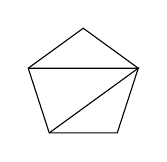
\begin{tikzpicture}[x=0.75pt,y=0.75pt,yscale=-0.5,xscale=0.5]
\draw (40.7,146.98) -- (93.72,108.46) -- (146.74,146.98) -- (126.49,209.31) -- (60.95,209.31) -- cycle ;
\draw (40.7,146.98) -- (146.74,146.98) -- (60.95,209.31);
\end{tikzpicture}
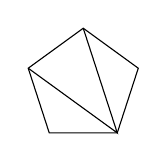
\begin{tikzpicture}[x=0.75pt,y=0.75pt,yscale=-0.5,xscale=0.5]
\draw (40.7,146.98) -- (93.72,108.46) -- (146.74,146.98) -- (126.49,209.31) -- (60.95,209.31) -- cycle ;
\draw (93.72,108.46) -- (126.49,209.31) -- (40.7,146.98);
\end{tikzpicture}
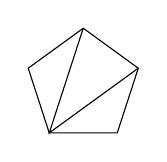
\begin{tikzpicture}[x=0.75pt,y=0.75pt,yscale=-0.5,xscale=0.5]
\draw (40.7,146.98) -- (93.72,108.46) -- (146.74,146.98) -- (126.49,209.31) -- (60.95,209.31) -- cycle ;
\draw (146.74,146.98) -- (60.95,209.31) -- (93.72,108.46);
\end{tikzpicture}
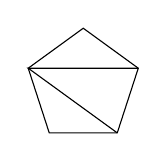
\begin{tikzpicture}[x=0.75pt,y=0.75pt,yscale=-0.5,xscale=0.5]
\draw (40.7,146.98) -- (93.72,108.46) -- (146.74,146.98) -- (126.49,209.31) -- (60.95,209.31) -- cycle ;
\draw (126.49,209.31) -- (40.7,146.98) -- (146.74,146.98);
\end{tikzpicture}
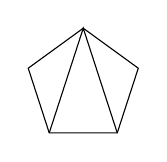
\begin{tikzpicture}[x=0.75pt,y=0.75pt,yscale=-0.5,xscale=0.5]
\draw (40.7,146.98) -- (93.72,108.46) -- (146.74,146.98) -- (126.49,209.31) -- (60.95,209.31) -- cycle ;
\draw (60.95,209.31) -- (93.72,108.46) -- (126.49,209.31);
\end{tikzpicture}
\caption*{5 Non-Overlapping Triangulations of a Pentagon}
\end{figure}

\begin{hl}
\begin{proof}
\;
\medskip

\begin{minipage}{0.69\linewidth}
Let $t_n$ count the number of triangulations of an $n$-gon. Pick an edge of the polygon. There are $n-2$ triangles it could belong to, since there are $n-2$ other vertices. In each case, it splits the polygon into two smaller ones with number of sides $k$ and $n+3-k$ for $2\leq k\leq n+1$. The number of ways to finish the triangulation is thus $t_{k-2}t_{n+1-k}$. Summing over all $k$, we have $\sum_{k=2}^{n+1}t_{k-2}t_{n+1-k}=\sum_{k=1}^{n}t_{k-1}t_{n-k}$. But this is the same recurrence as the Catalan Numbers in Theorem \ref{catalan_recur}. Since $t_2=1=c_0$ and $t_3=1=c_1$, we have that $t_{n+2}=c_n$.
\end{minipage}%
\begin{minipage}{0.3\linewidth}
\centering
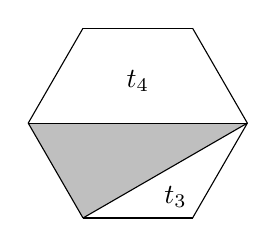
\begin{tikzpicture}[x=0.75pt,y=0.75pt,yscale=-0.4,xscale=0.4]
\path [fill=gray!50] (431.34,140.89) -- (233.39,255.18) -- (167.4,140.89) -- cycle;
\draw (431.34,140.89) -- (365.36,255.18);
\draw (365.36,255.18) -- (233.39,255.18);
\draw (233.39,255.18) -- (167.4,140.89);
\draw (167.4,140.89) -- (233.39,26.6);
\draw (233.39,26.6) -- (365.36,26.6);
\draw (365.36,26.6) -- (431.34,140.89);
\draw (431.34,140.89) -- (233.39,255.18);
\draw (431.34,140.89) -- (167.4,140.89);
\node at (299.375,90) {$t_4$};
\node at (345,230) {$t_3$};
\end{tikzpicture}
\end{minipage}

\medskip

Another proof bijects triangulations to full binary trees whose vertices are the $n+2$ exterior edges and the $n-1$ internal edges (resulting in $n+1$ leaf nodes). Fix an edge to be the root of the tree, and identify the triangle it belongs to. Let the other two edges be the children of the root. Now continue recursively. Any exterior edge encountered is a leaf node. For any internal edge, it borders two triangles: the one used to reach that edge, and a triangle not yet counted. Let the children of the edge be the other two edges of the uncounted triangle.

\medskip

A final proof bijects triangulations to parenthesizations. Label all except one of the edges, so that there are $n+1$ labeled edges. Now, iteratively label the interior edges by combining labels, using parentheses to specify the order in which they are combined. The final parenthesization is the label of the last exterior edge.

\begin{figure}[H]
\centering
\begin{subfigure}{0.6\linewidth}
\raisebox{-.5\height}{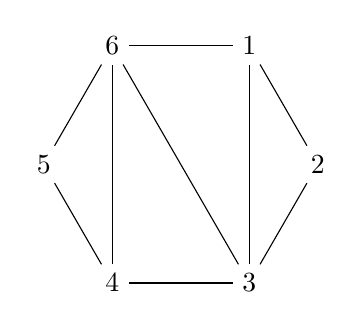
\begin{tikzpicture}[x=0.75pt,y=0.75pt,yscale=-0.5,xscale=0.5]
\node (1) at (431.34,140.89) {2};
\node (2) at (365.36,255.18) {3};
\node (3) at (233.39,255.18) {4};
\node (4) at (167.4,140.89) {5};
\node (5) at (233.39,26.6) {6};
\node (6) at (365.36,26.6) {1};
\path[-] (1) edge (2);
\path[-] (2) edge (3);
\path[-] (3) edge (4);
\path[-] (4) edge (5);
\path[-] (5) edge (6);
\path[-] (6) edge (1);
\path[-] (3) edge (5);
\path[-] (5) edge (2);
\path[-] (2) edge (6);
\end{tikzpicture}}
$\longleftrightarrow$
\raisebox{3.5\height}{\begin{forest}
[16
	[13
		[12]
		[23]
	]
	[36
		[34]
		[46
			[45]
			[46]
		]
	]
]
\end{forest}}
\caption*{Method 2}
\end{subfigure}%
\begin{subfigure}{0.3\linewidth}
\centering
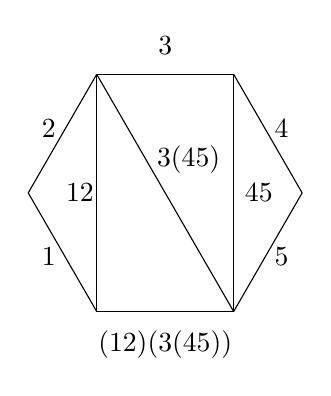
\begin{tikzpicture}[x=0.75pt,y=0.75pt,yscale=-0.5,xscale=0.5]
\draw   (431.34,140.89) -- (365.36,255.18) node [pos=0.3, label=below:{5}] {};
\draw (365.36,255.18) -- (233.39,255.18) node [pos=0.5, label=below:{(12)(3(45))}] {};
\draw (233.39,255.18) -- (167.4,140.89) node [pos=0.7, label=below:{1}] {};
\draw (167.4,140.89) -- (233.39,26.6) node [pos=0.3, label=2] {};
\draw (233.39,26.6) -- (365.36,26.6) node [pos=0.5, label=3] {};
\draw (365.36,26.6) -- (431.34,140.89) node [pos=0.7, label=4] {};
\draw (233.39,26.6) -- (365.36,255.18) node [pos=0.5, label=above right:{3(45)}, xshift=-1em] {};
\draw (233.39,26.6) -- (233.39,255.18) node [pos=0.5, label=left:{12}, xshift=0.6em] {};
\draw (365.36,26.6) -- (365.36,255.18) node [pos=0.5, label=right:{45}, xshift=-0.3em] {};
\end{tikzpicture}
\caption*{Method 3}
\end{subfigure}
\end{figure}
\end{proof}
\end{hl}
\end{theorem}

\begin{theorem}
Consider a string of parentheses that satisfies the criteria to be legal, except that not all left parentheses need to be closed. Let $q_n$ count the number of possible strings of length $n$. Then $q_n=\binom n{\lfloor n/2\rfloor}$, the Central Binomial Coefficients.

\begin{hl}
\begin{proof}
If no prefix exists, then removing the leading left parenthesis is a bijection to $q_{n-1}$. Otherwise, condition on the index, so that there are $\sum_{k=1}^{\lfloor n/2\rfloor}c_{k-1}q_{n-2k}$ options. Together, we have $q_n=q_{n-1}+\sum_{k=1}^{\lfloor n/2\rfloor}c_{k-1}q_{n-2k}$ for $n>0$ and $q_0=1$. The corresponding generating function is:
\begin{align*}
Q(x)
&=\sum_{n=0}^\infty q_nx^n
=q_0+\sum_{n=1}^\infty\left[q_{n-1}+\sum_{k=1}^{\lfloor n/2\rfloor}c_{k-1}q_{n-2k}\right]x^n
=1+\sum_{n=1}^\infty q_{n-1}x^n+\sum_{n=1}^\infty\sum_{k=1}^{\lfloor n/2\rfloor}c_{k-1}q_{n-2k}x^n\\
&=1+xQ(x)+\sum_{k=1}^{\infty}\sum_{n=2k}^\infty c_{k-1}q_{n-2k}x^n
=1+xQ(x)+\sum_{k=1}^{\infty}c_{k-1}x^{2k}\sum_{n=2k}^\infty q_{n-2k}x^{n-2k}\\
&=1+xQ(x)+Q(x)x^2\sum_{k=0}^{\infty}c_{k}x^{2k}
=1+xQ(x)+Q(x)x^2C(x^2)
\end{align*}

Solving:
\begin{align*}
Q(x)
&=-\frac{1}{x^2C(x^2)+x-1}
=-\frac{1}{\frac{1-\sqrt{1-4x^2}}{2}+x-1}
=\frac{2}{\sqrt{1-4x^2}-2x+1}\\
&=\frac{2(\sqrt{1-4x^2}+2x-1)}{(\sqrt{1-4x^2}-2x+1)(\sqrt{1-4x^2}+2x-1)}
=\frac{2\sqrt{1-4x^2}+4x-2}{1-4x^2-(2x-1)^2}
=\frac{2\sqrt{1-4x^2}+4x-2}{-8x^2+4x}\\
&=\frac{\sqrt{1-4x^2}+2x-1}{2x(1-2x)}
\end{align*}

Thus, using Theorem \ref{truncate_alt_binom}:
\begin{align*}
q_n
&=[x^n]Q(x)
=\frac12[x^n]\frac{\sqrt{1-4x^2}+2x-1}{x(1-2x)}
=\frac12[x^{n+1}]\left(\frac{\sqrt{1-4x^2}}{1-2x}-1\right)
=\frac12[x^{n+1}]\frac{\sqrt{1-4x^2}}{1-2x}\\
&=2^n[x^{n+1}]\frac{\sqrt{1-x^2}}{1-x}
=2^n\sum_{k=0}^{n+1}[x^k](1-x^2)^{1/2}
=2^n\sum_{k=0}^{n+1}[x^k]\sum_{k=0}^\infty\binom{1/2}k(-1)^kx^{2k}\\
&=2^n\sum_{k=0}^{n+1}[x^k]\sum_{k=0}^\infty[k\text{ even}]\binom{1/2}{k/2}(-1)^{k/2}x^{k}
=2^n\sum_{\substack{k=0\\k\text{ even}}}^{n+1}\binom{1/2}{k/2}(-1)^{k/2}\\
&=2^n\sum_{k=0}^{\lfloor\frac{n+1}2\rfloor}\binom{1/2}{k}(-1)^{k}
=2^n\binom{-1/2}{\lfloor(n+1)/2\rfloor}(-1)^{\lfloor(n+1)/2\rfloor}
=2^{n-2\lfloor\frac{n+1}2\rfloor}\binom{2\lfloor\frac{n+1}2\rfloor}{\lfloor\frac{n+1}2\rfloor}
\end{align*}

When $n$ is even, we obtain $\binom n{n/2}$. When $n$ is odd, we obtain $\frac12\binom{n+1}{(n+1)/2}=\frac12\frac{n+1}{(n+1)/2}\binom{n}{(n-1)/2}=\binom n{(n-1)/2}$. In either case, $q_n=\binom n{\lfloor n/2\rfloor}$.
\end{proof}
\end{hl}
\end{theorem}

\subsection{Counting Using Products and Compositions}
%\begin{theorem}\label{count_w_prod}
%Let $a_n$ count the number of ways to build an $\alpha$-structure on an $n$-element set and $b_n$ count the number of ways to build a $\beta$-structure on an $n$-element set. The product of their ordinary generating functions $A(x)B(x)$ has counts the number of ways to divide $[n]$ into two intervals, build an $\alpha$-structure on the first interval, and build a $\beta$-structure on the second interval.
%\begin{arrows}
%\item This follows directly from the definition of multiplication for power series
%\end{arrows}
%\end{theorem}

\begin{example}
Suppose a semester of $n$ days is divided into two parts (of arbitrary length), and there is 1 holiday during the first part and 2 holidays during the second part. Let $s_n$ be the number of ways this can be accomplished. If the first part has $k$ days, then there are $a_k=k$ ways to select the holiday. If the second part has $k$ days, then there are $b_k=\binom k2$ ways to select the two holidays. By Lemma \ref{binom_gen}:
\begin{equation*}
S(x)
=A(x)B(x)
=\frac{x}{(1-x)^2}\cdot \frac{x^2}{(1-x)^3}
=\frac{x^3}{(1-x)^5}
\end{equation*}

Thus, we compute:
\begin{equation*}
s_n
=[x^n]\frac{x^3}{(1-x)^5}
=[x^n]\frac1x\frac{x^4}{(1-x)^5}
=[x^{n+1}]\frac{x^4}{(1-x)^5}
=\binom{n+1}4
\end{equation*}
\end{example}

\begin{example}
Consider dividing a group of people into subgroups $A$, $B$, and $C$, and ask each subgroup to form a line. We also require that $A$ have an odd number of people, and that $B$ have an even number of people. We count the number of ways to do this. The exponential generating function representing the number of ways to arrange $n$ people in group $A$ is $A(x)=\sum_{n=0}^\infty\frac{1-(-1)^n}2n!\frac{x^n}{n!}=\sum_{n=0}^\infty\frac{1-(-1)^n}2x^n=\frac12\left[\sum_{n=0}^\infty x^n-\sum_{n=0}^\infty(-x)^n\right]=\frac12\left[\frac1{1-x}-\frac1{1+x}\right]$. The exponential generating function representing the number of ways to arrange $n$ people in group $B$ is $B(x)=\sum_{n=0}^\infty\frac{1+(-1)^n}2n!\frac{x^n}{n!}=\frac12\left[\frac1{1-x}+\frac1{1+x}\right]$. The remaining generating function is $C(x)=\sum_{n=0}^\infty x^n=\frac1{1-x}$. The total number of ways is thus encoded in the exponential generating function:
\begin{align*}
A(x)B(x)C(x)
&=\frac12\left[\frac1{1-x}-\frac1{1+x}\right]\frac12\left[\frac1{1-x}+\frac1{1+x}\right]\frac1{1-x}
=\frac14\left[-\frac{2x}{x^2-1}\right]\left[-\frac2{x^2-1}\right]\frac1{1-x}\\
&=\frac{-x}{(x+1)^2(x-1)^3}
=\frac{-1/16}{x+1}+\frac{-1/8}{(x+1)^2}+\frac{1/16}{x-1}+\frac{-1/4}{(x-1)^3}
\end{align*}

Then, we have:
\begin{align*}
[x^n]A(x)B(x)C(x)
&= -\frac1{16}[x^n]\frac{1}{x+1}-\frac18[x^n]\frac{1}{(x+1)^2}+\frac1{16}[x^n]\frac{1}{x-1}-\frac14[x^n]\frac{1}{(x-1)^3}\\
&= -\frac1{16}(-(-1)^{n+1})
-\frac18\left((-1)^{n+2}\binom{n+1}{1}\right)
+\frac1{16}(-(1)^{n+1})
-\frac14\left(-(1)^{n+3}\binom{n+2}2\right)\\
&= \frac1{16}(-1)^{n+1}
+\frac18(-1)^{n+1}(n+1)
-\frac1{16}
+\frac18(n+2)(n+1)\\
&= \frac1{16}[(-1)^{n+1}-1]
+\frac18(n+1)[n+2+(-1)^{n+1}]
\end{align*}

Since this is an exponential generating function, the total number of ways is:
\begin{equation*}
n!\left[\frac1{16}[(-1)^{n+1}-1]
+\frac18(n+1)[n+2+(-1)^{n+1}]\right]
=
\left\{
\begin{NiceArray}{ll}
\frac{n!\cdot n(n+2)}8&\text{if }n\text{ is even}\\
\frac{(n+1)!\cdot(n+3)}8&\text{if }n\text{ is odd}
\end{NiceArray}
\right.
\end{equation*}
\end{example}

\begin{example}
Consider counting the number of ways to make change for a given amount $n$. The number of ways with solely pennies is $[x^n]\sum_{k=0}^\infty x^k=\frac1{1-x}$, with solely nickels is $[x^n]\sum_{k=0}^\infty x^{5k}=\frac1{1-x^5}$, and so on. Thus, the product $\frac1{1-x}\frac1{1-x^5}\frac1{1-x^{10}}\cdots$ counts the number of ways to make change for $n$ with any combination of coins.

\medskip

This can also work with a finite bank of coins by truncating each power series (instead of using an infinite series).
\end{example}

\subsection{Snake Oil Method}

\begin{concept}
The \emph{Snake Oil Method} uses generating functions to compute sums containing a free variable. First, a free variable $n$ is identified and the sum is named $g_n$. The generating function $G(x)$ is written, which now contains two summations. Interchange the order of summation, then try to identify the coefficients in this new form.
\begin{arrows}
\item The name points to the fact that this method may or may not work, and when it does work, it may seem miraculous or not easily explainable
\end{arrows}
\end{concept}

\begin{example}
Consider the summation $a_n=\displaystyle\sum_{k=0}^\infty\binom{n+k}{mk}\alpha^{n-k}$ for some $n,m\in\N$ and $\alpha\in\R$. Its generating function with respect to $n$ is $\displaystyle A(x)=\frac{\alpha(1-\alpha x)^{m-1}}{(1-\alpha x)^m-(\alpha x)^{m-1}}$, which can be used to find the closed form of $a_n$ depending on the value of $m$ and $\alpha$. For example, when $m=2$ and $\alpha=2$, we obtain $a_n=\frac13(1+2\cdot4^n)$.

\begin{hl}
\begin{proof}
Using the free variable $n$, we have:
\begin{align*}
A(x)
&=\sum_{n=0}^\infty\sum_{k=0}^\infty\binom{n+k}{mk}\alpha^{n-k}x^n
=\sum_{k=0}^\infty\alpha^{-k}\sum_{n=0}^\infty\binom{n+k}{mk}(\alpha x)^n\\
&=\sum_{k=0}^\infty\alpha^{-k}(\alpha x)^{-k}\sum_{n=0}^\infty\binom{n+k}{mk}(\alpha x)^{n+k}
=\sum_{k=0}^\infty\alpha^{-k}(\alpha x)^{-k}\sum_{n=k}^\infty\binom{n}{mk}(\alpha x)^{n}\\
&\overset{\ref{sum_bin_times_monom}}=\sum_{k=0}^\infty\alpha^{-k}(\alpha x)^{-k}\frac{(\alpha x)^{mk}}{(1-\alpha x)^{mk+1}}
=\frac1{1-\alpha x}\sum_{k=0}^\infty\left(\frac{(\alpha x)^{m-1}}{\alpha(1-\alpha x)^m}\right)^k
=\frac1{1-\alpha x}\frac{1}{1-\frac{(\alpha x)^{m-1}}{\alpha(1-\alpha x)^m}}\\
&=\frac1{1-\alpha x}\frac{\alpha(1-\alpha x)^m}{\alpha(1-\alpha x)^m-(\alpha x)^{m-1}}
=\frac{\alpha(1-\alpha x)^{m-1}}{\alpha(1-\alpha x)^m-(\alpha x)^{m-1}}
\end{align*}

Consider the case where $m=2$ and $\alpha=2$. Then $A(x)=\frac{1-2 x}{(1-2 x)^2-x}=\frac{1-2x}{1-5x+4x^2}$. Then:
\begin{equation*}
a_n=[x^n]\frac{1-2x}{1-5x+4x^2}
=[x^n]\left(\frac{1/3}{1-x}+\frac{2/3}{1-4x}\right)
=\frac13(1+2\cdot4^n)\qedhere
\end{equation*}
\end{proof}
\end{hl}
\end{example}

\begin{example}
Consider the summation $\sum_{k=0}^\infty\binom nk\binom{2n}{n-k}$. This is equal to $\binom{3n}n$ by Vandermonde's Identity, but we can also use the Snake Oil Method. Using $n$ as the free variable results in the summation $\sum_{k=0}^\infty\binom{2n}{n-k}\frac{x^k}{(1-x)^{k+1}}$, which is not particularly nice to evaluate. Instead, if we add a free variable $m$ so that $a_n=\sum_{k=0}^\infty\binom nk\binom{m}{n-k}$, then we can proceed with the generating function with respect to $m$:
\begin{align*}
A(x)
&=\sum_{m=0}^\infty\sum_{k=0}^\infty\binom nk\binom{m}{n-k}x^m
=\sum_{k=0}^\infty\binom nk\sum_{m=0}^\infty\binom{m}{n-k}x^m
=\sum_{k=0}^\infty\binom nk\frac{x^{n-k}}{(1-x)^{n-k+1}}\\
&=\frac{x^n}{(1-x)^{n+1}}\sum_{k=0}^\infty\binom nk\left(\frac{1-x}x\right)^k
=\frac{x^n}{(1-x)^{n+1}}\left(1+\frac{1-x}x\right)^n
=\frac{1}{(1-x)^{n+1}}
\end{align*}

Thus, $a_{n}=[x^{2n}]\frac{1}{(1-x)^{n+1}}=\binom{3n}n$.
\end{example}

\begin{example}
$\displaystyle\sum_{k=0}^\infty\binom{2n+1}{2p+2k+1}\binom{p+k}k=4^{n-p}\binom{2n-p}{p}$

\begin{hl}
\begin{proof}
Let $s=2n+1$, and consider the generating function with respect to $s$:
\begin{align*}
S(x)
&=
\sum_{s=0}^\infty\sum_{k=0}^\infty\binom{s}{2p+2k+1}\binom{p+k}kx^s
=\sum_{k=0}^\infty\binom{p+k}p\sum_{s=0}^\infty\binom{s}{2p+2k+1}x^s\\
&=\sum_{k=0}^\infty\binom{p+k}p\frac{x^{2p+2k+1}}{(1-x)^{2p+2k+2}}
=\sum_{k=p}^\infty\binom{k}p\frac{x^{2k+1}}{(1-x)^{2k+2}}
=\frac x{(1-x)^2}\sum_{k=p}^\infty\binom{k}p\left(\frac{x^{2}}{(1-x)^{2}}\right)^k\\
&=\frac x{(1-x)^2}\frac{\left(\frac{x^{2}}{(1-x)^{2}}\right)^{p}}{\left(1-\frac{x^{2}}{(1-x)^{2}}\right)^{p+1}}
=\frac x{(1-x)^2}\left(\frac{x^{2}}{(1-x)^{2}}\right)^{p}\left(\frac{(1-x)^{2}}{1-2x}\right)^{p+1}
= \frac{x^{2p+1}}{(1-2x)^{p+1}}
\end{align*}

Extracting the coefficients:
\begin{align*}
[x^s]\frac{x^{2p+1}}{(1-2x)^{p+1}}
&=[x^{s-2p-1}]\frac{1}{(1-2x)^{p+1}}
=(-2)^{-p-1}[x^{s-2p-1}]\frac{1}{(x-1/2)^{p+1}}\\
&=(-2)^{-p-1}\left(\frac1{1/2}\right)^{(s-2p-1)+(p+1)}\binom{(s-2p-1)+(p+1)-1}{(p+1)-1}(-1)^{p+1}\\
&=2^{s-2p-1}\binom{s-p-1}{p}
=2^{2n-2p}\binom{2n-p}{p}
=4^{n-p}\binom{2n-p}p\qedhere
\end{align*}
\end{proof}
\end{hl}
\end{example}

\begin{example}
$\displaystyle\sum_{k=0}^\infty\binom{2n+1}{2k}\binom{m+k}{2n}=\binom{2m+1}{2n}$

\begin{hl}
\begin{proof}
Consider the generating function in $m$:
\begin{align*}
A(x)
&=\sum_{m=0}^\infty\sum_{k=0}^\infty\binom{2n+1}{2k}\binom{m+k}{2n}x^m
=\sum_{k=0}^\infty\binom{2n+1}{2k}\sum_{m=0}^\infty\binom{m+k}{2n}x^m\\
&=\sum_{k=0}^\infty\binom{2n+1}{2k}x^{-k}\sum_{m=0}^\infty\binom{m+k}{2n}x^{m+k}
=\sum_{k=0}^\infty\binom{2n+1}{2k}x^{-k}\sum_{m=k}^\infty\binom{m}{2n}x^{m}
\end{align*}

In order for a term in the original sum to be nonzero, we must have $k\leq n$, so that $k<2k\leq 2n$. Thus, we may change the index of the above summation to be $m=0$, since all terms introduced will have $\binom m{2n}=0$. Then:

\begin{align*}
A(x)
&=\sum_{k=0}^\infty\binom{2n+1}{2k}x^{-k}\sum_{m=0}^\infty\binom{m}{2n}x^{m}
=\sum_{k=0}^\infty\binom{2n+1}{2k}x^{-k}\frac{x^{2n}}{(1-x)^{2n+1}}\\
&=\sum_{k=0}^n\binom{2n+1}{2n+1-2k}\frac{x^{2n-k}}{(1-x)^{2n+1}}
=\sum_{k=0}^n\binom{2n+1}{2(n-k)+1}\frac{x^{n+(n-k)}}{(1-x)^{2n+1}}\\
&=\sum_{k=0}^n\binom{2n+1}{2k+1}\frac{x^{n+k}}{(1-x)^{2n+1}}
=\frac{x^n}{(1-x)^{2n+1}}\sum_{k=0}^n\binom{2n+1}{2k+1}x^k
\end{align*}

Now consider the generating function in $y=\sqrt x$:
\begin{align*}
B(x)
&=\frac{y^{2n}}{(1-y^2)^{2n+1}}\sum_{k=0}^n\binom{2n+1}{2k+1}y^{2k}
=\frac{y^{2n-1}}{(1-y^2)^{2n+1}}\sum_{k=0}^n\binom{2n+1}{2k+1}y^{2k+1}\\
&=\frac{y^{2n-1}}{(1-y)^{2n+1}(1+y)^{2n+1}}\frac{(1+y)^{2n+1}-(1-y)^{2n+1}}2
=\frac{y^{2n-1}}{2(1-y)^{2n+1}}-\frac{y^{2n-1}}{2(1+y)^{2n+1}}\\
&=\frac1{2y}\left[\frac{y^{2n}}{(1-y)^{2n+1}}-\frac{y^{2n}}{(1+y)^{2n+1}}\right]
\end{align*}

Thus:
\begin{align*}
[x^m]A(x)
&=[y^{2m}]B(x)
=[y^{2m}]\frac1{2y}\left(\frac{y^{2n}}{(1-y)^{2n+1}}-\frac{y^{2n}}{(1+y)^{2n+1}}\right)\\
&=\frac12\left([y^{2m+1}]\frac{y^{2n}}{(1-y)^{2n+1}}-[y^{2m+1}]\frac{y^{2n}}{(1+y)^{2n+1}}\right)\\
&=\frac12\left([y^{2m+1}]\frac{y^{2n}}{(1-y)^{2n+1}}-[(-y)^{2m+1}]\frac{(-y)^{2n}}{(1-y)^{2n+1}}\right)\\
&=\frac12\left([y^{2m+1}]\frac{y^{2n}}{(1-y)^{2n+1}}+[y^{2m+1}]\frac{y^{2n}}{(1-y)^{2n+1}}\right)
=[y^{2m+1}]\frac{y^{2n}}{(1-y)^{2n+1}}
=\binom{2m+1}{2n}\qedhere
\end{align*}
\end{proof}
\end{hl}
\end{example}

\section{Combinatorial Classes}

\begin{definition}
A combinatorial \emph{class} is a finite or countable set of objects with a size defined for each object in the set satisfying:
\begin{itemize}
\item The size of each object is a nonnegative integer
\item The number of objects of a given size is finite
\end{itemize}

If $\mathcal A$ is such as class, then the size of $a\in\mathcal A$ is denoted $|a|$.
\end{definition}

\begin{definition}
We can associate an ordinary generating function with a combinatorial class $\mathcal A$ by:
\begin{equation*}
\sum_{a\in\mathcal A}x^{|a|}
=\sum_{n\geq 0}A_nx^n\text{ where }A_n\text{ is the subset of }\mathcal A\text{ containing objects of size }n
\end{equation*}

$\{A_n\}$ is called the \emph{counting sequence}.
\end{definition}

\begin{example}
Consider permutations on $[5]$, and let the size of a permutation $\pi\in S_5$ be given by its inversion number. Consider the combinatorial class $\mathcal B=\{21345, 21354, 12453, 14523, 41325, 51243\}$. The inversion numbers are $(1,2,4,4,5)$ respectively, so that the ogf is $B(x)=x^1+2x^2+2x^4+x^5$ and the counting sequence is $\{0,1,2,0,2,1\}$.
\end{example}

\begin{example}
Consider the following collection of finite graphs, and let the size of a graph be given by its order (number of vertices):

\begin{figure}[H]
\centering
\begin{subfigure}{0.1\linewidth}
\centering
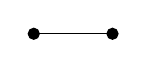
\begin{tikzpicture}
\coordinate (A) at (0,0);
\coordinate (B) at (1,0);
\draw (A) -- (B);
\foreach \vertex in {A,B}
    \filldraw (\vertex) circle (2pt);
\end{tikzpicture}
\end{subfigure}
\begin{subfigure}{0.1\linewidth}
\centering
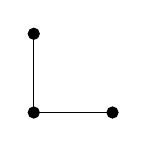
\begin{tikzpicture}
\coordinate (A) at (0,0);
\coordinate (B) at (1,0);
\coordinate (C) at (0,1);
\draw (C) -- (A) -- (B);
\foreach \vertex in {A,B,C}
    \filldraw (\vertex) circle (2pt);
\end{tikzpicture}
\end{subfigure}
\begin{subfigure}{0.1\linewidth}
\centering
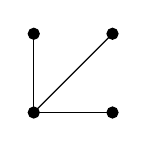
\begin{tikzpicture}
\coordinate (A) at (0,0);
\coordinate (B) at (1,0);
\coordinate (C) at (0,1);
\coordinate (D) at (1,1);
\draw (C) -- (A) -- (B);
\draw (A) -- (D);
\foreach \vertex in {A,B,C,D}
    \filldraw (\vertex) circle (2pt);
\end{tikzpicture}
\end{subfigure}
\begin{subfigure}{0.1\linewidth}
\centering
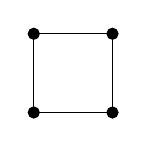
\begin{tikzpicture}
\coordinate (A) at (0,0);
\coordinate (B) at (1,0);
\coordinate (C) at (1,1);
\coordinate (D) at (0,1);
\draw (A) -- (B) -- (C) -- (D) -- (A);
\foreach \vertex in {A,B,C,D}
    \filldraw (\vertex) circle (2pt);
\end{tikzpicture}
\end{subfigure}
\begin{subfigure}{0.1\linewidth}
\centering
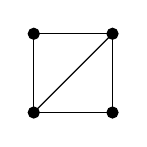
\begin{tikzpicture}
\coordinate (A) at (0,0);
\coordinate (B) at (1,0);
\coordinate (C) at (1,1);
\coordinate (D) at (0,1);
\draw (A) -- (B) -- (C) -- (D) -- (A);
\draw (A) -- (C);
\foreach \vertex in {A,B,C,D}
    \filldraw (\vertex) circle (2pt);
\end{tikzpicture}
\end{subfigure}
\begin{subfigure}{0.15\linewidth}
\centering
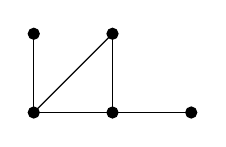
\begin{tikzpicture}
\coordinate (A) at (0,0);
\coordinate (B) at (1,0);
\coordinate (C) at (1,1);
\coordinate (D) at (0,1);
\coordinate (E) at (2,0);
\draw (D) -- (A) -- (B) -- (C);
\draw (A) -- (C);
\draw (B) -- (E);
\foreach \vertex in {A,B,C,D,E}
    \filldraw (\vertex) circle (2pt);
\end{tikzpicture}
\end{subfigure}
\end{figure}

Then the ordinary generating function is $C(x)=x^2+x^3+3x^4+x^5$. We could also use a bivariate generating function, with the exponent on $x$ representing the number of vertices and the exponent on $y$ representing the number of edges. This gives $K(x,y)=x^2y+x^3y^2+x^4y^3+x^4y^4+x^4y^5+x^5y^5$.
\end{example}

\begin{definition}
Two classes $\mathcal A$ and $\mathcal B$ are called \emph{equivalent} if the counting sequences are identical.
\end{definition}

\begin{definition}
The power of combinatorial classes is that we construct more complicated structures from simpler classes iteratively, and using generating functions, obtain the sizes of these new classes. A construction is called \emph{admissible} if the counting sequence $\{A_n\}$ of $\mathcal A$ only depends on the counting sequence of $B_n^1,B_n^2,\dots$ and not on any internal structure of any $B_n^k$, and also yields a valid combinatorial class satisfying the required properties.
\begin{arrows}
\item For example, $\mathcal A=\mathcal B\cup\mathcal C$ is not an admissible construction because it relies on knowledge of the elements of $\mathcal B$ and $\mathcal C$, rather than just their counting sequences
\end{arrows}
\end{definition}

\begin{definition}
Define two basic classes as follows:
\begin{itemize}
\item The \emph{neutral class} $\mathcal E=\{\square\}$, where $|\square|=0$. The corresponding generating function is $E(x)=1$.
\item The \emph{atomic class} $\mathcal Z=\{\cdot\}$, where $|\cdot|=1$. For example, $Z_a=\{a\}$ with $|a|=1$. The corresponding generating function is $Z(x)=x$.
\end{itemize}
\end{definition}

\begin{definition}
Define the following constructions:
\begin{itemize}
\item \emph{Cartesian Product}: $\mathcal A=\mathcal B\times\mathcal C=\{(b,c)|b\in\mathcal B,c\in\mathcal C\}$ using the size $|a|_{\mathcal A}=|b|_{\mathcal B}+|c|_{\mathcal C}$ (i.e., add the component sizes). The generating function is $A(x)=B(x)C(x)$.
\begin{arrows}
\item We allow for infinite Cartesian products as well, but only when any term of the resulting counting sequence depends on finitely many terms in the product. With this constraint, it is clear that the construction is admissible.
\item This Cartesian product ultimately represents a Cauchy product. It counts the number of ways to build two combinatorial structures whose sizes add to a particular value. In other words, we split $[n]$ into two intervals, build one structure on the left half, and build a second structure on the right half.
\end{arrows}
\item \emph{Combinatorial Sum}: $\mathcal A=\mathcal B+\mathcal C=(\{\triangle\}\times B)\cup(\{\diamond\}\times C)$ using the size $|(\triangle,a)|_{\mathcal A}=|a|_{\mathcal B}$ and $|(\diamond,a)|_{\mathcal A}=|a|_{\mathcal C}$. The generating function is $A(x)=B(x)+C(x)$.
\begin{arrows}
\item This is effectively a union, but we ensure the two sets are disjoint by multiplying with arbitrary $\triangle$ and $\diamond$.
\end{arrows}
\item \emph{Sequence Construction}: Assume $\square\not\in\mathcal B$. Then $\operatorname{SEQ}(\mathcal B)=\mathcal E+B+B\times B+B^3+\cdots$. The ordinary generating function for the $\mathcal A=\operatorname{SEQ}(\mathcal B)$ is $A(x)=1+B(x)+B^2(x)+\cdots=\frac1{1-B(x)}$.
\begin{arrows}
\item $\mathcal E$ allows selection of the empty sequence and $B^k$ allows for sequences of length $k$.
\item If $\mathcal B$ contained $\square$, then there would be an infinite number of objects of any given size, generated by inserting arbitrary many $\square$ elements.
\item We also define $\operatorname{SEQ}_k(\mathcal B)=\mathcal B^k$, which are sequences of fixed length. The ordinary generating function is $B(x)^k$.
\item $\operatorname{SEQ}_{\leq k}(\mathcal B)=\sum_{j=0}^k\mathcal B_j$ has the generating function $\frac{1-B(x)^{k+1}}{1-B(x)}$
\item $\operatorname{SEQ}_{\geq k}(\mathcal B)=\sum_{j=k}^\infty\mathcal B_j$ has the generating function $\frac{B(x)^k}{1-B(x)}$
\item For $\Omega\subset\W$, let $\operatorname{SEQ}_{\Omega}(\mathcal B)$ represent sequences whose lengths are in $\Omega$. This has generating function $\sum_{k\in\Omega}B(x)^k$
\end{arrows}
\item \emph{Cycle Construction}: Assume $\square\not\in\mathcal B$. Define an equivalence relation $S$ between sequences, where two sequences are equivalent if there exists a cyclic permutation (circular shift) mapping one to the other (ignoring the initial arbitrary element $\triangle$, $\diamond$, etc.). Then $\operatorname{CYC}(\mathcal B)=(\operatorname{SEQ}(\mathcal B)\setminus\{\square\})/S$. The ordinary generating function for $\mathcal A=\operatorname{CYC}(\mathcal B)$ is $A(x)=\sum_{k=1}^\infty\frac{\phi(k)}k\log\left(\frac1{1-B(x^k)}\right)$, where $\phi$ is the Euler totient function.
\begin{arrows}
\item The empty sequence is excluded by convention.
\item We also define $\operatorname{CYC}_k(\mathcal B)=(\operatorname{SEQ}_k(\mathcal B)\setminus\{\square\})/S$, which are cycles of fixed length. %todo generating function
\end{arrows}
\item \emph{Multiset Construction}: Assume $\square\not\in\mathcal B$. Define an equivalence relation $\Pi$ between sequences, where two sequences are equivalent if there exists an arbitrary permutation mapping one to the other (ignoring the initial arbitrary element $\triangle$, $\diamond$, etc.). Then $\operatorname{MSET}(\mathcal B)=\operatorname{SEQ}(B)/\Pi$. The ordinary generating function for $\mathcal A=\operatorname{MSET}(\mathcal B)$ is $A(x)=\prod_{n=1}^\infty(1-x^n)^{-B_n}=\exp\sum_{k=1}^\infty\frac{B(x^k)}k$.
\begin{arrows}
\item We also define $\operatorname{MSET}_k(\mathcal B)=\operatorname{SEQ}_k(\mathcal B)/\Pi$, which are multisets of fixed size. %todo generating function
\end{arrows}
\item \emph{Powerset Construction}: Assume $\square\not\in\mathcal B$. $\operatorname{PSET}(\mathcal B)\subset\operatorname{MSET}(\mathcal B)$ with the restriction that all elements are distinct (ignoring the initial arbitrary element $\triangle$, $\diamond$, etc.). Define this similarly for $\operatorname{PSET}_k(\mathcal B)$. The ordinary generating function for $\mathcal A=\operatorname{PSET}(\mathcal B)$ is $A(x)=\prod_{n=1}^\infty(1+x^n)^{B_n}=\exp\sum_{k=1}^\infty\frac{(-1)^{k-1}B(x^k)}k$.
\begin{arrows}
\item We also define $\operatorname{PSET}_k(\mathcal B)$ similarly, which are subsets of a fixed size. %todo generating function
\end{arrows}
\end{itemize}

\begin{hl}
\begin{proof}
For the Cartesian product, we have:
\begin{equation*}
A(x)
=\sum_{n=0}^\infty A_nx^n
=\sum_{n=0}^\infty\sum_{k=0}^nB_kC_{n-k}x^n
\overset{\text{III}}=B(x)C(x)
\end{equation*}

For an infinite Cartesian product, we note that any initial finite number of terms can be correctly captured with a finite product. Thus, the infinite product is a valid formal power series, and is the limit of the partial products.

\medskip

For the sum construction, we have:
\begin{equation*}
A(x)=\sum_{a\in\mathcal A}x^{|a|_{\mathcal A}}
=\sum_{a\in(\{\triangle\}\times B)\cup(\{\diamond\}\times C)}x^{|a|_{\mathcal A}}
=\sum_{b\in\mathcal B}x^{|a|_{\mathcal B}}+\sum_{c\in\mathcal C}x^{|c|_{\mathcal C}}
=B(x)+C(x)
\end{equation*}

For the sequence construction, start by noting that $\frac1{1-B(x)}$ is a valid composition of power series since $[x^0]B(x)=0$. Formally, we have an infinite combinatorial sum, but we can show similarly to the above proof that the resulting generating function is the infinite sum of the generating functions. Hence, the result follows immediately.

\medskip

For the cycle construction, consider any nonempty sequence in $\operatorname{SEQ}(\mathcal B)$, and note that it has a unique root which is primitive. For example, if $\mathcal B=\{\alpha,\beta\}$, the sequence $\alpha\beta\alpha\beta\beta\alpha\beta\alpha\beta\beta\alpha\beta\alpha\beta\beta$ decomposes uniquely into $\alpha\beta\alpha\beta\beta|\alpha\beta\alpha\beta\beta|\alpha\beta\alpha\beta\beta$ where $\alpha\beta\alpha\beta\beta$ cannot be decomposed into a word repeated multiple times (and hence is called primitive). We use a bivariate generating function to describe $\operatorname{SEQ}_{\geq1}(\mathcal B)$, with $z$ tracking the size as normal, and $u$ tracking the length of the sequence. The resulting generating function is thus $\frac{uB(z)}{1-uB(z)}$. Letting $PS(z,u)$ be the generating function representing primitive sequences over $\mathcal B$ only, we have $\frac{uB(z)}{1-uB(z)}=\sum_{k=1}^\infty PS(z^k,u^k)$, where $k$ conditions on the number of times the root is repeated.

\medskip

Apply M\"obius Inversion to obtain $PS(z,u)=\sum_{k=1}^\infty \mu(k)\frac{u^kB(z^k)}{1-u^kB(z^k)}$. More formally, consider any term of the power series, written as $[z^{in}u^{jn}]$ for coprime $i,j$. Let $a_n=[z^{in}u^{jn}]\frac{uB(z)}{1-uB(z)}$ and $b_n=[z^{in}u^{jn}]PS(z,u)$. Then the previous equality gives us the following, from which we can apply M\"obius Inversion and obtain equality for all $i,j$ (so that the bivariate power series are equal):
\begin{align*}
a_n
&=\sum_{k=1}^\infty[z^{in}u^{jn}]PS(z^k,u^k)
=\sum_{k|in\text{ and }k\mid jn}[z^{in}u^{jn}]PS(z^k,u^k)
=\sum_{k|n}[z^{in}u^{jn}]PS(z^k,u^k)\\
&=\sum_{k|n}[z^{in/k}u^{jn/k}]PS(z,u)
=\sum_{k|n}[z^{ik}u^{jk}]PS(z,u)
=\sum_{k|n}b_k
\end{align*}

Next, notice that each primitive $k$-cycle has $k$ distinct primitive word representations. So, the generating function $PC(z,u)$ for the number of primitive $k$-cycles has coefficients $[z^nu^k]PS(z,u)/k$, which can be obtained through the integral $\int_0^uPS(z,t)/t\,dt$. Substituting and using a $u$-substitution gives $PC(z,u)=\sum_{k=1}^\infty\frac{\mu(k)}k\log\frac1{1-u^kB(z^k)}$.

\medskip

To count the number of primitive cycles of given size without conditioning on their length, substitute $u\gets1$ to obtain $PC(z)=\sum_{k=1}^\infty\frac{\mu(k)}k\log\frac1{1-B(z^k)}$. Every cycle has a unique root which is a primitive cycle, so that the generating function for $\operatorname{CYC}(\mathcal B)$ satisfies $C(z)=\sum_{k=1}^\infty PC(z^k)$, where again $k$ conditions on the number of times the root is repeated. So, we obtain:
\begin{equation*}
C(z)
=\sum_{k=1}^\infty\sum_{j=1}^\infty\frac{\mu(j)}j\log\frac1{1-B(z^{jk})}
=\sum_{n=1}^\infty\sum_{j|n}\frac{\mu(j)}j\log\frac1{1-B(z^n)}
=\sum_{n=1}^\infty\frac{\phi(n)}n\log\frac1{1-B(z^n)}
\end{equation*}

We used Corollary \ref{totient_multiplicative} to simplify $\sum_{j|n}\frac{\mu(j)}j$ and obtain the result.

\medskip

For the multiset construction, order $\mathcal B$, so that every equivalence class in $\mathcal A=\operatorname{MSET}(\mathcal B)$ can be represented by a sequence whose elements are in order. Thus, $\mathcal A=\prod_{b\in\mathcal B}\operatorname{SEQ}(\{b\})$. Thus:
\begin{align*}
A(x)
&=\prod_{b\in\mathcal B}\frac1{1-x^{|b|}}
=\prod_{n=1}^\infty\frac1{(1-x^n)^{B_n}}
=\exp\left(-\sum_{n=1}^\infty B_n\log(1-x^n)\right)
=\exp\left(\sum_{n=1}^\infty\sum_{k=1}^\infty B_n\frac{(x^n)^k}{k}\right)\\
&=\exp\left(\sum_{k=1}^\infty\frac1k\sum_{n=1}^\infty B_n(x^k)^n\right)
=\exp\sum_{k=1}^\infty\frac1kB(x^k)
\end{align*}

For the powerset construction, note that $\mathcal A=\operatorname{PSET}(\mathcal B)\cong\prod_{b\in\mathcal B}(\{\square\}+\{b\})$, where $\square$ represents not including an element $b$ in the final set. Thus:
\begin{align*}
A(x)
&=\prod_{b\in\mathcal B}(1+x^{|b|})
=\prod_{n=1}^\infty(1+x^n)^{B_n}
=\exp\sum_{n=1}^\infty B_n\log(1+x^n)
=\exp\sum_{n=1}^\infty B_n\sum_{k=1}^\infty(-1)^{k+1}\frac{(x^n)^k}k\\
&=\exp\sum_{k=1}^\infty\frac{(-1)^{k+1}}k\sum_{n=1}^\infty B_n(x^k)^n
=\exp\sum_{k=1}^\infty\frac{(-1)^{k+1}}kB(x^k)
\end{align*}

In the multiset and powerset constructions, since $B_0=0$, the infinite product used above is admissible.
\end{proof}
\end{hl}
\end{definition}

\begin{theorem}
Consider combinatorial classes $\mathcal B$ and $\mathcal C$ with corresponding generating functions $B$ and $C$. Assume $b_0=0$. Then $C(B(x))$ counts the number of ways to partition $[n]$ into intervals, build a $\mathcal B$-structure on each interval, and build a $\mathcal C$-structure on the set of intervals.

\begin{hl}
\begin{proof}
Let $\mathcal A$ be the combinatorial class describing the number of ways to accomplish this. By the definition of the product, $\mathcal B^k$ is the combinatorial class describing the number of ways to divide $[n]$ into $k$ intervals and build a $\mathcal B$-structure on each. The corresponding generating function is $B^k(x)$. The number of ways to build a $\mathcal C$-structure on the intervals is $c_kB^k(x)$. Sum over all $k$ to obtain the result.
\end{proof}
\end{hl}
\end{theorem}

\begin{example}
Let $\mathcal Z=\{\cdot\}$ be an atomic class. Let $\mathcal B=\{\mathcal Z,\mathcal Z\times\mathcal Z\}=\{\cdot,(\cdot,\cdot)\}$, so that $B(x)=x+x^2$. Now we can form $\mathcal A=\operatorname{SEQ}(\mathcal B)$ and obtain $A(x)=\frac1{1-x-x^2}$. This is the generating function for the Fibonacci numbers, which can be understood by associating $\cdot$ with monominoes and $(\cdot,\cdot)$ with dominoes.
\end{example}

\begin{example}
More generally, consider $\mathcal B_{j,k}=\mathcal Z^j+\mathcal Z^k$ with generating function $x^j+x^k$. Then the generating function for $\mathcal A=\operatorname{SEQ}(\mathcal B_{j,k})$ is $A(x)=\frac1{1-x^j-x^k}$. We could then consider $\mathcal C=\operatorname{SEQ}(\mathcal A\setminus\mathcal E)$, which represents sequences of the $j$-omino and $k$-omino tilings. We have $C(x)=\frac1{1-(\frac1{1-x^j-x^k}-1)}=\frac{1-x^j-x^k}{1-2x^j-2x^k}$.
\end{example}

\begin{example}
Let $\mathcal Z=\{\cdot\}$ be an atomic class. Let $\mathcal N=\operatorname{SEQ}(\mathcal Z)\setminus\{\square\}$, which is the combinatorial class corresponding to the natural numbers with size function being the identity. The corresponding generating function is $N(x)=\frac1{1-x}-1$. Now consider $\mathcal A=\operatorname{SEQ}(\mathcal N)$, so that $A(x)=\frac1{1-(\frac1{1-x}-1)}=\frac{1-x}{1-2x}=\frac12\cdot\frac1{1-2x}+\frac12$. For $n\geq1$, we thus have $[x^n]A(x)=2^{n-1}$, which is the number of compositions of $n$. For $n=0$, there is also one composition, reflected by $[x^0]A(x)=1$.
\end{example}

\begin{example}
Consider $b\operatorname{SEQ}(a)$, which is words starting with a $b$ and followed by an arbitrary number of copies of $a$. This is a Cartesian product of $\{b\}$ and $\operatorname{SEQ}(a)$, so that the generating function is $x\cdot\frac1{1-x}=\frac x{1-x}$. Then $\operatorname{SEQ}(b\operatorname{SEQ}(a))$, which is all words over $\{a,b\}$ starting with $b$, has the generating function $\frac1{1-\frac x{1-x}}=\frac{1-x}{1-2x}$. Notice that this is equivalent to $\operatorname{SEQ}(\mathcal N)$, since we can view the $b$ letters as delimiting a sequence of natural numbers.

\medskip

To count all words over $\{a,b\}$, we use $\operatorname{SEQ}(a)\operatorname{SEQ}(b\operatorname{SEQ}(a))$, which has the generating function $\frac1{1-x}\cdot\frac{1-x}{1-2x}=\frac1{1-2x}$. This satisfies $[x^n]\frac1{1-2x}=2^n$ as expected.
\end{example}

\newcommand{\drawVDots}[1]{
	\raisebox{1pt}{
  \begin{tikzpicture}[y=3mm]
    \foreach \i in {1,...,#1} {
      \fill (0,\i-1) circle[radius=2pt];
    }
    \draw (0,0) -- (0,#1-1);
  \end{tikzpicture}}
}

\begin{example}
Let $\mathcal B=\{\drawDots{1},\drawDots{1}\,\drawDots{2},\drawDots{3}\}$, which is shorthand for $\mathcal B=\{\cdot,(\cdot,(\cdot,\cdot)),(\cdot,\cdot,\cdot)\}$, or a combinatorial class with one element of size 1 and two elements of size 3. The five elements of size 4 in $\mathcal A=\operatorname{SEQ}(\mathcal B)$ are:
\begin{equation*}
\begingroup
\def\arraystretch{0.8}
\arraycolsep=0pt
\drawVDots{3}\drawVDots{1},
\begin{array}[b]{c}\drawVDots{2}\\\drawVDots{1}\end{array}\drawVDots{1},
\drawVDots{1}\drawVDots{3},
\drawVDots{1}\begin{array}[b]{c}\drawVDots{2}\\\drawVDots{1}\end{array},
\drawVDots{1}\drawVDots{1}\drawVDots{1}\drawVDots{1}
\endgroup
\end{equation*}

The generating function for $\mathcal A$ is $\frac1{1-x-2x^3}$. If we wish to find the generating function of $\operatorname{SEQ}(\drawDots{2}\mathcal A)$, then we obtain:
\begin{equation*}
\frac1{1-x^2\cdot\frac1{1-x-2x^3}}
=\frac{1-x-2x^3}{1-x-x^2-2x^3}
\end{equation*}
\end{example}

\begin{example}
Suppose $\mathcal A=\mathcal Z^k\times\operatorname{SEQ}(\mathcal A)$. Then the generating function satisfies $A(x)=\frac{x^k}{1-A(x)}$. Rearranging and solving with the quadratic formula yields $A(x)=\frac{1-\sqrt{1-4x^k}}2=x^kC(x^k)$, where $C(x)$ is the generating function for the Catalan numbers given in Lemma \ref{catalan_gen}.
\end{example}

\begin{definition}
For an element $a$ of size $|a|$, the \emph{weight} of $a$ is $x^{|a|}$. More generally, we can consider weights that involve multiple variables, such as assigning a weight of $x^{\alpha}y^{\beta}$. Normally, the weight is a multiple of $x^{|a|}$, either a constant multiple or a multiple that is a monomial in other variables. Similar to the restriction on sizes for combinatorial classes, we must have that there are a finite number of elements of any given weight. Given this, we denote the resulting \emph{weighted combinatorial class} by $\mathcal A_{\wt}$.

\medskip

A \emph{weighted generating function} $A_{\wt}$ is formed by summing the weights of all elements, so that:
\begin{equation*}
A_{\wt}(x_1,\dots,x_m)=\sum_{a\in\mathcal A_{\wt}}\wt(a)
\end{equation*}
\end{definition}

\begin{proposition}
If $B_{\wt}$ and $C_{\wt}$ are weighted combinatorial classes, then $B_{\wt}+C_{\wt}$ and $B_{\wt}\times C_{\wt}$ are admissible, and $\operatorname{SEQ}(B_{\wt})$ is as well assuming that $\square\not\in B_{\wt}$.
\end{proposition}

\begin{example}
Let $\mathcal S$ be the collection of ordered pairs $([n],A)$ where $A\subset[n]$ and $n>0$. Let the size of $([n],A)$ be $n$. We have $\mathcal S\cong\operatorname{SEQ}(\{0,1\})$ with $|0|=|1|=1$. Indeed, the length of the sequence corresponds to $n$, with $0$ representing excluded elements and $1$ representing included elements. The ordinary generating function is $S(x)=\frac1{1-2x}$.

\medskip

We now form a weighted generating function where the weight of $([n],A)$ is $x^ny^{|A|}$. $\wt(0)=x$ and $\wt(1)=xy$. Therefore, the weighted generating function becomes:
\begin{equation*}
S_{\wt}(x,y)
=\frac1{1-(x+xy)}
=\sum_{n=0}^\infty(x+xy)^n
=\sum_{n=0}^\infty x^n(1+y)^n
=\sum_{n=0}^\infty\sum_{k=0}^n\binom nk y^kx^n
\end{equation*}
\end{example}

\begin{example}
We can use the above weighted generating function to derive Pascal's identity (a recurrence for the binomial coefficient). We have $1=(1-x-xy)\sum_{n=0}^\infty\sum_{k=0}^n\binom nk y^kx^n$. Apply $[x^ny^k]$ with $(n,k)\neq(0,0)$ to each side to obtain:
\begin{align*}
0
&=[x^ny^k]\sum_{n=0}^\infty\sum_{k=0}^n\binom nk x^ny^k
-[x^ny^k]x\sum_{n=0}^\infty\sum_{k=0}^n\binom nk x^ny^k
-[x^ny^k]xy\sum_{n=0}^\infty\sum_{k=0}^n\binom nk x^ny^k\\
&=[x^ny^k]\sum_{n=0}^\infty\sum_{k=0}^n\binom nk x^ny^k
-[x^{n-1}y^k]\sum_{n=0}^\infty\sum_{k=0}^n\binom nk x^ny^k
-[x^{n-1}y^{k-1}]\sum_{n=0}^\infty\sum_{k=0}^n\binom nk x^ny^k\\
&=\binom nk-\binom{n-1}k-\binom{n-1}{k-1}
\end{align*}

Rearranging then yields the result.
\end{example}

\begin{example}
We can also use the weighted generating function to show the Binomial Theorem, namely $(1+y)^n=\sum_{k=0}^n\binom nky^k$. Rewrite $\frac1{1-(x+xy)}=\frac1{1-x(1+y)}=\sum_{n=0}^\infty (1+y)^nx^n$. Applying $[x^n]$ yields $(1+y)^n$, and applying $[x^n]$ to the equivalent quantity $\sum_{n=0}^\infty\sum_{k=0}^n\binom nkx^ny^k$ yields $\sum_{k=0}^n\binom nky^k$ as desired.
\end{example}

\section{Labeled Structures}

\begin{definition}
A \emph{labeled structure} is a function $\mathcal S$ which maps each finite set $L$ to a finite multiset $\mathcal S(L)$ such that if $|L|=|M|$, then $|\mathcal S(L)|=|\mathcal S(M)|$. The set $L$ is called the \emph{labels} and $\mathcal S(L)$ is the \emph{structure} on $L$.

\medskip

Suppose that $|L|=n$, and let $s_n=|S(L)|$. The corresponding exponential generating function is $F_{\mathcal S}(x)=F_{\mathcal S(\cdot)}(x)=\sum_{n=0}^\infty s_n\frac{x^n}{n!}$.

\begin{arrows}
\item From another point of view, we can view labeled structures as an endowment of additional information onto combinatorial classes. Consider a combinatorial class $\mathcal A$. However, for each $a\in\mathcal A$, we associate to it $|a|$ labels. The number of ways to label the structure $a$ must only depend on $|a|$, and we denote it $s_{|a|}$.
\end{arrows}
\end{definition}

\begin{concept}
The reason for making $\mathcal S(L)$ a multiset rather than a set arises due to complications arising with products of labeled structures. See Example \ref{multiset_label} for an example. When $\mathcal S(L)\cap \mathcal S(M)=\varnothing$ for distinct $L\neq M$, then we can let $\mathcal S(L)$ simply be a set rather than a multiset. If we desire to only work with sets rather than multisets, we can modify the definition of problematic structures that do not satisfy $S(L)\cap S(M)=\varnothing$ by endowing each $S\in\mathcal S(L)$ with knowledge of its original label set $L$. In other words, we define the equivalent combinatorial structure $\tilde{\mathcal S}(L)=\{(S,L)\mid S\in\mathcal S(L)\}$.
\end{concept}

\begin{definition}
$\mathcal S$ and $\mathcal T$ are \emph{equivalent}, denotes $\mathcal S\equiv\mathcal T$, if $|\mathcal S(L)|=|\mathcal T(L)|$ for all finite $L$.
\end{definition}

\begin{definition}
Let $\mathcal S$ and $\mathcal T$ be labeled structures. If $\mathcal S(L)$ and $\mathcal T(L)$ are disjoint for any finite $L$, then $\mathcal S$ and $\mathcal T$ are called \emph{disjoint}.
\end{definition}

\begin{definition}
For disjoint $\mathcal S$ and $\mathcal T$, define their \emph{sum} as $(\mathcal S\cup\mathcal T)(L)=\mathcal S(L)\cup\mathcal T(L)$. Since all unions are disjoint, this is a valid labeled structure.
\end{definition}

\begin{definition}
Let $\mathcal S,\mathcal T$ be labeled structures. Then their \emph{product} is:
\begin{align*}
(\mathcal S\times\mathcal T)(L)
&=\{(S,T)\mid S\in\mathcal S(L_1),T\in\mathcal T(L_2)\text{ where }(L_1,L_2)\text{ is a weak partition of }L\}\\
&=\bigcup_{k=0}^{\infty}\left\{(S,T)\mid S\in\mathcal S(L_1),T\in\mathcal T(L\setminus L_1),L_1\in\binom Lk\right\}
\end{align*}

Note that the above union is finite for any fixed $L$. $L_1$ or $L_2$ may be empty. We also denote the weak partition by $L_1/L_2\vdash L$. This counts the number of ways to divide the labels in $L$ between the two structures $S$ and $T$, and then form valid labelings/structures on each structure.
\begin{arrows}
\item It may be possible to obtain the same tuple with different values of $L_1$ and $L_2$, which is why we must consider the above as a multiset.
\end{arrows}
\end{definition}

\begin{proposition}
Let $\mathcal S$ and $\mathcal T$ be labeled structures with exponential generating functions $F_{\mathcal S}$ and $F_{\mathcal T}$. For $|L|=n$, $s_n=|\mathcal S(L)|$, and $t_n=|\mathcal T(L)|$, we have:
\begin{enumerate}
\item $|(\mathcal S\cup\mathcal T)(L)|=s_n+t_n$ assuming that $\mathcal S$ and $\mathcal T$ are disjoint. $F_{\mathcal S\cup\mathcal T}(x)=F_{\mathcal S}(x)+F_{\mathcal T}(x)$.
\item $|(\mathcal S\times\mathcal T)(L)|=\sum_{k=0}^n\binom nks_kt_{n-k}$ and $F_{\mathcal S\times\mathcal T}(x)=F_{\mathcal S}(x)F_{\mathcal T}(x)$.
\end{enumerate}

\begin{hl}
\begin{proof}
$|(\mathcal S\cup\mathcal T)(L)|=s_n+t_n$ holds since $\mathcal S$ and $\mathcal T$ are disjoint. The formula for the exponential generating functions thus follows immediately.

\medskip

$|(\mathcal S\times\mathcal T)(L)|=\sum_{k=0}^n\binom nks_kt_{n-k}$ follows by conditioning on $k=|L_1|$, picking the values of $L_1$ $\binom nk$ ways, and then forming the $\mathcal S$-structure $s_k$ ways and the $\mathcal T$-structure $t_{n-k}$ ways. Now apply Wilf III to obtain the corresponding formula for the exponential generating functions.
\end{proof}
\end{hl}
\end{proposition}

\begin{definition}
Define the \emph{partition structure} of $\mathcal S$ as:
\begin{equation*}
\Pi(\mathcal S)(L)=\{\{S_1,S_2,\dots\}\mid L_1/L_2/\cdots\vdash L\text{ and }S_j\in\mathcal S(L_j)\}
\end{equation*}

Under this structure, we partition $L$ in all possible ways, and then build an $\mathcal S$-structure on each block in all possible ways. Note that we must have $\mathcal S(\varnothing)=\varnothing$, so that $|\mathcal S(\varnothing)|=0$. Otherwise, the partition structure would map finite sets to infinite sets (since partitions could be empty).
\begin{arrows}
\item This is akin to the definition of a product, but order does not matter (and the number of factors is arbitrary)
\end{arrows}
\end{definition}

\begin{theorem}
Suppose the exponential generating function of a labeled structure $\mathcal S$ is $F_{\mathcal S}(x)=\sum_{n=1}^\infty s_n\frac{x^n}{n!}$. Note that $s_0=0$. Then:
\begin{equation*}
F_{\Pi(\mathcal S)}(x)
=e^{F_{\mathcal S}(x)}
=\sum_{n=0}^\infty\frac{F_{\mathcal S}(x)^n}{n!}
\end{equation*}

\begin{hl}
\begin{proof}
Condition on the number of blocks in the partition:
\begin{equation*}
\Pi(\mathcal S)(L)
=\bigcup_{n=0}^\infty\{\{S_1,\dots,S_n\}\mid L_1/\cdots/L_n\vdash L\text{ and }S_j\in\mathcal S(L_j)\}
\end{equation*}

Since $s_0=0$, the above union is finite for all $L$. Fix any $n$:
\begin{align*}
&|\{\{S_1,\dots,S_n\}\mid L_1/\cdots/L_n\vdash L\text{ and }S_j\in\mathcal S(L_j)\}|
=\frac1{n!}|\{(S_1,\dots,S_n)\mid L_1/\cdots/L_n\vdash L\text{ and }S_j\in\mathcal S(L_j)\}|\\
&\quad=\frac1{n!}|\mathcal S^n(L)|
\end{align*}

Hence, the exponential generating function for the single term is $F_{\mathcal S}(x)^n/n!$. Sum over all $n$ to obtain the result.
\end{proof}
\end{hl}
\end{theorem}

\begin{theorem}\label{exp_comp}
More generally, suppose we have a labeled structure $\mathcal S$ and a labeled structure $\mathcal T$ with exponential generating functions $F_{\mathcal S}$ and $F_{\mathcal T}$. Assume $s_0=0$ and $t_0=1$. Then $F_{\mathcal S}(F_{\mathcal T}(x))$ counts the number of ways to partition $L$ into any number of blocks, build a $\mathcal T$-structure within each block, and build a $\mathcal S$-structure on the set of blocks.

\begin{arrows}
\item This immediately implies the previous result, where the structure we build on each block is merely itself (labeled structure $E$, with exponential generating function $e^x$)
\end{arrows}

\begin{hl}
\begin{proof}
Let $F(x)=F_{\mathcal S}(F_{\mathcal T}(x))$ be the exponential generating function for $\{f_n\}$, representing the labeled structure:
\begin{equation*}
\mathcal F(L)=\bigcup\{\mathcal T(\{S_1,S_2,\dots\})\mid L_1/L_2/\cdots\vdash L\text{ and }S_j\in\mathcal S(L_j)\}
\end{equation*}

Condition on the number of blocks in the partition:
\begin{equation*}
\mathcal F(L)=\bigcup_{n=0}^\infty\bigcup\{\mathcal T(\{S_1,\dots,S_n\})\mid L_1/\cdots/L_n\vdash L\text{ and }S_j\in\mathcal S(L_j)\}
\end{equation*}

Fix any $n$:
\begin{align*}
&\left|\bigcup\{\mathcal T(\{S_1,\dots,S_n\})\mid L_1/\cdots/L_n\vdash L\text{ and }S_j\in\mathcal S(L_j)\}\right|\\
&\quad=t_n\left|\{\{S_1,\dots,S_n\}\mid L_1/\cdots/L_n\vdash L\text{ and }S_j\in\mathcal S(L_j)\}\right|\\
&\quad=\frac{t_n}{n!}\left|\{(S_1,\dots,S_n)\mid L_1/\cdots/L_n\vdash L\text{ and }S_j\in\mathcal S(L_j)\}\right|
=\frac{t_n}{n!}|\mathcal S^n(L)|
\end{align*}

Hence, the exponential generating function for the single term is $F_{\mathcal S}(x)^n\cdot t_n/n!$. Sum over all $n$ to obtain the result.
%
%Let $\Pi_n$ be the set of partitions of $[n]$. When the index of summation is $(T_1,\dots,T_k)$, we sum over disjoint nonempty subsets of $[n]$ whose union is $[n]$. When the index of summation is $(t_1,\dots,t_k)$, we sum over $t_i\geq1$ adding to $n$. Then for $n\geq1$:
%\begin{align*}
%f_n
%&=\sum_{k=1}^nb_k\sum_{\{T_1,\dots,T_k\}\in\Pi_n}a_{|T_1|}\cdots a_{|T_k|}
%=\sum_{k=1}^n\frac{b_k}{k!}\sum_{(T_1,\dots,T_k)}a_{|T_1|}\cdots a_{|T_k|}\\
%&=\sum_{k=1}^n\frac{b_k}{k!}\sum_{(t_1,\dots,t_k)}\binom{n}{t_1,\dots,t_k}a_{t_1}\cdots a_{t_k}
%\end{align*}
%
%Hence:
%\begin{align*}
%F(x)
%&=1+\sum_{n=1}^\infty\frac{x^n}{n!}\sum_{k=1}^n\frac{b_k}{k!}\sum_{(t_1,\dots,t_k)}\binom{n}{t_1,\dots,t_k}a_{t_1}\cdots a_{t_k}\\
%&=1+\sum_{k=1}^\infty\frac{b_k}{k!}\sum_{n=k}^\infty \frac{x^n}{n!}\sum_{(t_1,\dots,t_k)}\binom{n}{t_1,\dots,t_k}a_{t_1}\cdots a_{t_k}
%\overset{\text{III}}=1+\sum_{k=1}^\infty\frac{b_k}{k!}\sum_{n=k}^\infty\left([x^n](A(x))^k\right)x^n\\
%&\overset{a_0=0}=1+\sum_{k=1}^\infty\frac{b_k}{k!}\sum_{n=0}^\infty\left([x^n](A(x))^k\right)x^n
%=1+\sum_{k=1}^\infty\frac{b_k}{k!}A(x)^k\qedhere
%=B(A(x))
%\end{align*}
\end{proof}
\end{hl}
\end{theorem}

\begin{example}\label{example_binom_label}
Consider $\mathcal S(L)=\binom Lk$, where $k\in\W$. Then $s_n=\binom nk$, so that:
\begin{equation*}
F_{\binom{\cdot}k}(x)
=\sum_{n=0}^\infty\binom nk\frac{x^n}{n!}
=\sum_{n=k}^\infty\binom nk\frac{x^n}{n!}
=\sum_{n=k}^\infty\frac{1}{k!(n-k)!}x^n
=\frac{x^k}{k!}\sum_{n=k}^\infty\frac{x^{n-k}}{(n-k)!}
=\frac{x^k}{k!}e^x
\end{equation*}
\end{example}

\begin{example}\label{powerset_label}
Consider the powerset structure $\mathcal P$. Then $s_n=2^n$, so that $F_{\mathcal P}=\sum_{n=0}^\infty 2^n\frac{x^n}{n!}=e^{2x}$. We can write the powerset structure as a sum of disjoint labeled structures:
\begin{equation*}
\mathcal S(L)=\bigcup_{k=0}^{|L|}\binom Lk
\end{equation*}

By the sum formula and Example \ref{example_binom_label}, we similarly derive $F_{\mathcal P}=e^{2x}$.

\medskip

We could also, in theory, coerce this into a form utilizing the partition structure. A powerset can be counted by representing each element of the set as a singleton, then choosing whether this singleton is included or not in two ways. Hence, $\mathcal P=\Pi(\mathcal S)$, where $\mathcal S$ is the labeled structure corresponding to assigning a singleton to included or not included. Then $F_{\mathcal S}(x)=2x$, and $F_{\mathcal P}(x)=e^{2x}$.
\end{example}

\begin{example}
Consider $E(L)=\{L\}$, so that $s_n=1$ for all $n$. Then:
\begin{equation*}
F_E(x)
=\sum_{n=0}^\infty\frac{x^n}{n!}
=e^x
\end{equation*}
\end{example}

\begin{example}
Consider $\overline E$ such that $\overline E:L\mapsto\{L\}$ when $L\neq\varnothing$ and $\overline E(\varnothing)=\varnothing$ otherwise. Then $s_n=I[n>0]$. We thus have $F_{\overline E}(x)=e^x-1$.
\end{example}

\begin{example}
Suppose $T([n])$ counts the number of labeled trees. The number of labeled trees is $s_n=n^{n-2}$ for $n\geq1$ and $s_0=0$ by Lemma \ref{num_labeled_trees}. Hence, $F_T(x)=\sum_{n=1}^\infty n^{n-2}\frac{x^n}{n!}$.
\end{example}

\begin{example}\label{ex_set_part}
Suppose $L\mapsto\setbinom Lk$ gives set partitions on $L$ of size $k$. Then $s_n=\setbinom nk$, so that $F_{\setbinom{\cdot}k}=\sum_{n=0}^\infty\setbinom nk\frac{x^n}{n!}=\frac{(e^x-1)^k}{k!}$ by Proposition \ref{set_part_exp}. Multiplying by $k!$ gives us the exponential generating function $(e^x-1)^k$ for ordered set partitions of $L$ into $k$ parts.
\end{example}

\begin{example}
Suppose $L\mapsto\mathcal S(L)$ gives ordered set partitions of $L$. Then $F_{\mathcal S}=\frac1{2-e^x}$ by Lemma \ref{ordered_part_exp_gen}.
\end{example}

\begin{example}
Suppose $L\mapsto\mathcal S(L)$ gives permutations on $L$. Then $s_n=n!$, so that $F_{\mathcal S}=\sum_{n=0}^\infty n!\frac{x^n}{n!}=\sum_{n=0}^\infty x^n=\frac1{1-x}$.
\end{example}

\begin{example}
Suppose $L\mapsto\sqbinom Lk$, which are permutations with exactly $k$ cycles. Then $s_n=\sqbinom nk$, so that $F_{\sqbinom{\cdot}k}=\frac1{k!}\left(\log\frac1{1-x}\right)^k$ by Proposition \ref{sqbinom_exp_gen}.

\medskip

In particular, when $k=1$, we obtain $F_{\sqbinom{\cdot}1}=\log\frac1{1-x}$.
\end{example}

\begin{example}\label{multiset_label}
Consider the labeled structure $(\mathcal P\times\mathcal P)(L)$. The exponential generating function is $e^{4x}$ by Example \ref{powerset_label} and the product formula, so that $|(\mathcal P\times\mathcal P)(L)|=4^{|L|}$. Take $L=[2]$, and we obtain $|(\mathcal P\times\mathcal P)([2])|=16$. Note, however, that the resulting $(\mathcal P\times\mathcal P)([2])$ is a multiset with duplicate entries. $(\varnothing,\varnothing)$ is generated by four different partitions of $L$: $\varnothing/12$, $1/2$, $2/1$, and $12/\varnothing$.

\medskip

The cause of this issue is that from any $S\in\mathcal S(L)$, it is not possible to recover $L$. In other words, there exists $L\neq M$ such that $\mathcal S(L)=\mathcal S(M)$.
\end{example}

\begin{example}
The labeled structure of ordered set partitions into $k$ parts is equivalent to $(\overline E)^k$.

\begin{hl}
\begin{proof}
Let the former be $\mathcal S$. To show this equivalence, we must prove $|\mathcal S(L)|=|(\overline E)^k(L)|$ for all finite $L$. In particular, we can show this by forming a bijection between $\mathcal S(L)$ and $(\overline E)^k(L)$. An ordered set partition can be viewed as a $k$-tuple of disjoint nonempty sets whose union is $L$. $\overline E(L)$ is the labeled structure for nonempty sets containing all elements in $L$, so that $(\overline E)^k(L)$ are tuples of nonempty sets containing disjoint elements, whose union is $L$. Hence, we have an obvious bijection.

\medskip

We can use this, for example, to show $\setbinom n2=2^{n-1}-1$. The labeled structure of ordered set partitions into 2 parts is equivalent to $(\overline E)^2$, so by the product rule has EGF $F(x)=(e^x-1)^2=e^{2x}-2e^x+1$. For $n\geq 1$, $[x^n]F(x)=2^n-2$. Divide by two to remove the order, yielding $\setbinom n2=2^{n-1}-1$.
\end{proof}
\end{hl}
\end{example}

\begin{example}
The labeled structure $\sqbinom Lk$ with ordered cycles is equivalent to $\sqbinom L1^k$.

\begin{hl}
\begin{proof}
We can view the ordered cycles in a $k$-tuple, where each element is a nonempty cycle with distinct values in $L$, such that all elements in $L$ are in at least one cycle. Each element of the tuple is represented by the labeled structure $\sqbinom L1$, so that we have an obvious bijection.

\medskip

We can use this, for example, to show $\sqbinom{n+1}2=n!\sum_{k=1}^n\frac1k$. The labeled structure $\sqbinom L2$ with ordered cycles is equivalent to $\sqbinom L1^2$. $\sqbinom L1$ has the exponential generating function $\log\frac1{1-x}$ since there are $(n-1)!$ permutations of $[n]$ with one cycle, so that the exponential generating function for $\sqbinom L2$ is $\left(\log\frac1{1-x}\right)^2$ by the product rule. Now use Wilf III and partial fraction decomposition to obtain:
\begin{align*}
\setbinom{n+1}2
&=\frac12\cdot(n+1)![x^{n+1}]\left(\log\frac1{1-x}\right)^2
=\frac12\cdot(n+1)!\sum_{k=1}^{n}\frac1k\frac1{n+1-k}\\
&=\frac12\cdot(n+1)!\frac1{n+1}\sum_{k=1}^n\left(\frac1k+\frac1{n+1-k}\right)
=n!\sum_{k=1}^n\frac1k\qedhere
\end{align*}
\end{proof}
\end{hl}
\end{example}

\begin{example}
The labeled structure $\mathcal P(\cdot)$ is equivalent to $E\times E$.

\begin{hl}
\begin{proof}
We can biject $A\leftrightarrow (A,L\setminus A)$ for any $A\in\mathcal P(L)$. Thus, we have a bijection from $\mathcal P(L)$ to $(E\times E)(L)$.
\end{proof}
\end{hl}
\end{example}

\begin{example}
For an example, we enumerate $\Pi(\setbinom\cdot 2)([5])$:
\begin{equation*}
\begin{array}{lllll}
\{1234/5\}&\{123/45\}&\{12/3,4/5\}&\{14/3,2/5\}&\{2/34,1/5\}\\
\{1235/4\}&\{124/35\}&\{13/2,4/5\}&\{1/34,2/5\}&\{23/5,1/4\}\\
\{1245/3\}&\{125/34\}&\{1/23,4/5\}&\{13/5,2/4\}&\{25/3,1/4\}\\
\{1345/2\}&\{134/25\}&\{12/4,3/5\}&\{15/3,2/4\}&\{2/35,1/4\}\\
\{1/2345\}&\{135/24\}&\{14/2,3/5\}&\{1/35,2/4\}&\{24/5,1/3\}\\
          &\{145/23\}&\{1/24,3/5\}&\{14/5,2/3\}&\{25/4,1/3\}\\
          &\{15/234\}&\{12/5,3/4\}&\{15/4,2/3\}&\{2/45,1/3\}\\
          &\{14/235\}&\{15/2,3/4\}&\{1/45,2/3\}&\{34/5,1/2\}\\
          &\{13/245\}&\{1/25,3/4\}&\{23/4,1/5\}&\{35/4,1/2\}\\
          &\{12/345\}&\{13/4,2/5\}&\{24/3,1/5\}&\{3/45,1/2\}
\end{array}
\end{equation*}
\end{example}

\begin{example}
Let $\mathcal S$ be the labeled structure of permutations, and let $\mathcal C(L)=\sqbinom L1$ be the labeled structure of single-cycle permutations. Then writing each permutation as a cycle decomposition, we can see $\mathcal S=\Pi(\mathcal C)$. In other words, we partition the elements in the permutation, then build a cycle on each block.

\medskip

We have $F_{\mathcal C}(x)=\log\frac1{1-x}$, so that $F_{\mathcal S}(x)=\exp(F_{\mathcal C}(x))=\frac1{1-x}$ as expected.
\end{example}

\section{Inversion Formulas}

\subsection{Binomial Inversion}

\begin{lemma}\label{bin_inv_prep_1}
$\displaystyle\sum_{k=0}^n\binom nk\binom km(-1)^k=(-1)^n\delta_{nm}$

\begin{arrows}
\item This is sometimes referred to as an \emph{orthogonality} condition, and is used in the development of the corresponding \emph{inversion} formulas
\end{arrows}

\begin{hl}
\begin{proof}
By Theorem \ref{extended_absorption} and Theorem \ref{alternating_binom}:
\begin{multline*}
\sum_{k=0}^n\binom nk\binom km(-1)^k
=\sum_{k=m}^n\binom nm\binom{n-m}{k-m}(-1)^k\\
=\binom nm(-1)^m\sum_{k=0}^{n-m}\binom{n-m}{k}(-1)^k
=\binom nm(-1)^m\delta_{nm}
=(-1)^n\delta_{nm}
\end{multline*}

Or, note that $\sum_{k=0}^n\binom nk\binom km$ counts the number of ordered pairs $(T,S)$ for $T\subset S\subset [n]$ and $|T|=m$. Let $E,\mathcal O$ be the sets for which $|S|$ is even or odd, respectively. If $n\leq m$, the result is trivial. Otherwise, form the involution $(T,S)\mapsto (T, S\,\triangle\,\max([n]\setminus T))$, i.e., add/remove to $S$ the largest element in $[n]$ that is not in $T$. This maps $E\leftrightarrow\mathcal O$, so we have the result.
\end{proof}
\end{hl}
\end{lemma}


\begin{theorem}[Binomial Inversion]\label{bin_inv}
Let $\{a_n\},\{b_n\}$ be sequences for $n\geq0$. Then:
\begin{equation*}
a_n=\sum_{k=0}^n\binom nkb_k\text{ for all }n\iff b_n=\sum_{k=0}^n\binom nka_k(-1)^{n-k}\text{ for all }n
\end{equation*}
\begin{arrows}
\item The symmetric version is $\displaystyle a_n=\sum_{k=0}^n\binom nkb_k(-1)^k$ iff $\displaystyle b_n=\sum_{k=0}^n\binom nka_k(-1)^k$
\item Binomial inversion can sometimes offer an alternative for proofs other than Inclusion/Exclusion, such as with derangements
\end{arrows}

\begin{hl}
\begin{proof}
Suppose the RHS. Using Lemma \ref{bin_inv_prep_1}:
\begin{align*}
\sum_{k=0}^n\binom nkb_k
&=\sum_{k=0}^n\binom nk\sum_{j=0}^k\binom kja_j(-1)^{k-j}
=\sum_{j=0}^na_j(-1)^{-j}\sum_{k=j}^n\binom nk\binom kj(-1)^k\\
&=\sum_{j=0}^na_j(-1)^{-j}(-1)^n\delta_{nj}
=a_n
\end{align*}

The converse and symmetric version follow by applying the above to modified versions of $a_n$ and $b_n$.

\medskip

Alternatively, we can use generating functions. Suppose RHS, and let $A$ and $B$ be the exponential generating functions of the sequences. Then using Proposition \ref{binom_exp}:
\begin{align*}
B(x)
&=\sum_{n=0}^\infty\frac{x^n}{n!}\sum_{k=0}^n\binom nka_k(-1)^{n-k}
=\sum_{k=0}^\infty(-1)^k a_k\sum_{n=k}^\infty\binom nk\frac{(-x)^n}{n!}\\
&=\sum_{k=0}^\infty(-1)^k a_k\frac{(-x)^k}{k!}e^{-x}
=e^{-x}\sum_{k=0}^\infty a_k\frac{x^k}{k!}
=e^{-x}A(x)
\end{align*}

Then by Wilf III, we have our result:
\begin{equation*}
A(x)
=e^xB(x)
=\sum_{n=0}^\infty\left(\sum_{k=0}^n\binom nkb_k\right)\frac{x^n}{n!}
\end{equation*}

The converse follows by applying the above to modified versions of $a_n$ and $b_n$.

\medskip

Instead of exponential generating function, we can use ordinary generating functions $A$ and $B$. By Theorem \ref{sum_bin_times_monom}, we have:
\begin{align*}
B(x)
&=\sum_{n=0}^\infty x^n\sum_{k=0}^n\binom nk a_k(-1)^{n-k}
=\sum_{k=0}^\infty (-1)^ka_k\sum_{n=k}^\infty \binom nk(-x)^n
=\sum_{k=0}^\infty (-1)^ka_k\frac{(-x)^k}{(1+x)^{k+1}}\\
&=\frac1{1+x}\sum_{k=0}^\infty a_k\left(\frac x{1+x}\right)^k
=\frac1{1+x}A\left(\frac x{1+x}\right)
\end{align*}

Take $x\gets\frac{x}{1-x}$ to obtain our result:
\begin{align*}
A(x)
&=\frac1{1-x}B\left(\frac{x}{1-x}\right)
=\frac1{1-x}\sum_{k=0}^\infty b_k\left(\frac{x}{1-x}\right)^k
=\sum_{k=0}^\infty b_k\frac{x^k}{(1-x)^{k+1}}\\
&=\sum_{k=0}^\infty b_k\sum_{n=0}^\infty\binom nk x^n
=\sum_{n=0}^\infty\left(\sum_{k=0}^n\binom nkb_k\right)x^n
\end{align*}

One can also view this as a consequence of M\"obius Inversion. Consider the poset $P$ of all subsets of $\N$ ordered by inclusion. Let $f(S)=b_{|S|}$ and $g(S)=a_{|S|}$. Then M\"obius inversion gives $g(T)=\sum_{S\subset T}f(S)$ iff $f(T)=\sum_{S\subset T}g(S)\mu(S,T)$. Letting $n=|T|$, conditioning on $k=|S|$, and noting that $\mu(S,T)=(-1)^{|T|-|S|}$ by Lemma \ref{boolean_mobius}, we have $a_n=\sum_{k=0}^n\binom nkb_k$ iff $b_n=\sum_{k=0}^n\binom nka_k(-1)^{n-k}$ as desired.

\medskip

As one final alternative, we can use Lagrange Inversion (not a preferred proof, but perhaps informative). We can derive $B(x)=\frac1{1+x}A(\frac x{1+x})$ as above. We let $y=\frac{x}{1+x}$, which can be rearranged as $x=y(1+x)=y\phi(x)$ for $\phi(x)=1+x$. Using this, $A(y)=(1+x)B(x)$, so taking $W(x)=(1+x)B(x)$, we have:
%
%By making the substitution $y=\frac{x}{1+x}$ or $x=\frac{y}{1-y}$, we obtained $A(y)=\frac1{1-y}B(\frac{y}{1-y})$. We can rewrite this as:
%\begin{equation*}
%A(y)=\frac1{1-y}B(\frac{y}{1-y})
%=\frac1{1-x/(1+x)}B\left(\frac{x/(1+x)}{1-x/(1+x)}\right)
%=(1+x)B(x)
%\end{equation*}
%
%In fact, the substitution we performed can be rewritten as $x(y)=y(1+x)=y\phi(x)$ for $\phi(x)=1+x$, which is reminiscent of Lagrange Inversion. Hence, we take $W(x)=(1+x)B(x)$ and thus have:
\begin{align*}
a_n
&=[x^n]A(x)
=\frac1n[z^{n-1}](W'(z)\phi(z)^n)
=\frac1n[z^{n-1}]\big((1+z)B'(z)+B(z)\big)(1+z)^n\\
&=\frac1n\sum_{k=0}^{n-1}[z^k]\big((1+z)B'(z)+B(z)\big)[z^{n-k-1}](1+z)^n\\
&=\frac1n\sum_{k=0}^{n-1}\big([z^k]B'(z)+[z^{k-1}]B'(z)+[z^k]B(x)\big)\binom{n}{n-k-1}\\
&=\frac1n\sum_{k=0}^{n-1}\big((k+1)b_{k+1}+kb_k+b_k\big)\binom{n}{k+1}
=\frac1n\sum_{k=0}^{n-1}(k+1)(b_{k+1}+b_k)\binom{n}{k+1}\\
&=\sum_{k=0}^{n-1}(b_{k+1}+b_k)\binom{n-1}{k}
=\sum_{k=0}^{n-1}b_k\binom{n-1}{k}+\sum_{k=0}^{n-1}b_{k+1}\binom{n-1}{k}\\
&=\sum_{k=0}^{n-1}b_k\binom{n-1}{k}+\sum_{k=1}^{n}b_{k}\binom{n-1}{k-1}
=\sum_{k=0}^{n}b_k\left(\binom{n-1}{k}+\binom{n-1}{k-1}\right)
=\sum_{k=0}^nb_k\binom nk\qedhere
\end{align*}
%
%
%
%We could take $W(x)=(1+x)B(x)$, but $W'(x)\phi(x)^n$ is difficult to work with.

%Instead, we expand:
%\begin{equation*}
%A(y)=B(x)+xB(x)=\sum_{k=0}^\infty b_kx(y)^k+\sum_{k=0}^\infty b_kx(y)^{k+1}
%\;\implies\;
%a_n=\sum_{k=0}^\infty b_k[y^n]x(y)^k+\sum_{k=0}^\infty b_k[y^n]x(y)^{k+1}
%\end{equation*}
%
%Now, we will use Lagrange Inversion to compute $[y^n]x(y)^k$ and $[y^n]x(y)^{k+1}$. Taking $W(x)=x^k$, we have:
%\begin{equation*}
%[y^n]x(y)^k
%=\frac1n[x^{n-1}]kx^{k-1}(1+x)^n
%=\frac kn[x^{n-k}](1+x)^n
%=\frac kn\binom nk
%=\binom{n-1}{k-1}
%\end{equation*}
%
%Similarly, taking $W(x)=x^{k+1}$, we have:
%\begin{equation*}
%[y^n]x(y)^{k+1}
%=\frac1n[x^{n-1}](k+1)x^{k}(1+x)^n
%=\frac{k+1}n[x^{n-k-1}](1+x)^n
%=\frac{k+1}n\binom n{k+1}
%=\binom{n-1}k
%\end{equation*}
%
%Combining these, $a_n=\sum_{k=0}^\infty b_k\left(\binom{n-1}{k-1}+\binom{n-1}k\right)=\sum_{k=0}^\infty\binom nkb_k$.
\end{proof}
\end{hl}
\end{theorem}

\begin{definition}
The \emph{binomial transform} of $\{a_n\}$ is $b_n=\sum_{k=0}^n\binom nka_k(-1)^k$.
\begin{arrows}
\item This is an involution, corresponding to the symmetric form of binomial inversion
\item We also have $b_n=(-1)^n(\delta^na)_0$, the $n$th forward difference with alternating sign
\item Sometimes the $(-1)^k$ is not included
\end{arrows}
\end{definition}

\begin{example}
Using Theorem \ref{surjection_count}, the binomial transform of $a_n=n^2$ is:
\begin{equation*}
b_n=\sum_{k=0}^n\binom nkk^2(-1)^k=(-1)^nn!\setbinom 2n=\{0,-1,2,0,0,\dots\}
\end{equation*}

This can also be found using the forward difference interpretation:
\begin{equation*}
\begin{array}{ccccccccc}
\boxed{0}&&1&&4&&9&&16\\
&\boxed{1}&&3&&5&&7\\
&&\boxed{2}&&2&&2\\
&&&\boxed{0}&&0
\end{array}
\end{equation*}
\end{example}

\begin{example}
The binomial transform of $a_n=1$ is:
\begin{equation*}
b_n=\sum_{k=0}^n\binom nka_k(-1)^k=\sum_{k=0}^n\binom nk(-1)^k=\delta_{n0}
\end{equation*}
\end{example}

\begin{example}
Using Extraction/Absorption, the binomial transform of $a_n=n$ is:
\begin{equation*}
b_n=\sum_{k=0}^n\binom nkk(-1)^k
=\sum_{k=1}^nn\binom{n-1}{k-1}(-1)^k
=-n\sum_{k=0}^{n-1}\binom{n-1}{k}(-1)^k
=-n\delta_{n1}
=-\delta_{n1}
\end{equation*}
\end{example}

\begin{example}
The binomial transform of $a_n=a^n$ is:
\begin{equation*}
b_n=\sum_{k=0}^n\binom nka^k(-1)^k=\sum_{k=0}^n\binom nk(-a)^k=(1-a)^n
\end{equation*}
\end{example}

\begin{example}
The binomial transform of $a_n=\delta_{n1}$ is:
\begin{equation*}
b_n=\sum_{k=0}^n\binom nk\delta_{k1}(-1)^k=\binom n1(-1)^1=-n
\end{equation*}
\end{example}

\subsection{Stirling Inversion}

\begin{lemma}\label{stirling_prep}
$\displaystyle \sum_{k=0}^n\sqbinom nk\setbinom km(-1)^{n-k}=\delta_{nm}$ and $\displaystyle \sum_{k=0}^n\setbinom nk\sqbinom km(-1)^{n-k}=\delta_{nm}$

\begin{arrows}
\item We use these claims to prove Stirling inversion. However, if the inversion is proved by other means, we could also derive these quickly from the Stirling inversion formulas.
\end{arrows}

\begin{hl}
\begin{proof}
We use Proposition \ref{sqbinom_gen} and Theorem \ref{monomial_as_falling}, which state that:
\begin{equation*}
x^{\overline n}=\sum_{k=0}^n\sqbinom nkx^k
\quad\text{and}\quad
x^n=\sum_{k=0}^n\setbinom nk(x)_k
\end{equation*}

We combine these to obtain:
\begin{align*}
x^n
&=\sum_{k=0}^n\setbinom nk(x)_k
=\sum_{k=0}^n\setbinom nk(-x)^{\overline k}(-1)^k
=\sum_{k=0}^n\setbinom nk\sum_{m=0}^k\sqbinom km(-x)^m(-1)^k\\
&=\sum_{m=0}^n\left(\sum_{k=m}^n\setbinom nk\sqbinom km(-1)^{k-m}\right)x^m
\end{align*}

Hence, we have our second result, after rewriting $(-1)^{k-m}=(-1)^{m-k}$ and then multiplying each side of the claim by $(-1)^{m-n}$. For the first claim:
\begin{align*}
(-x)^{\overline n}
&=\sum_{k=0}^n\sqbinom nk(-x)^k
=\sum_{k=0}^n\sqbinom nkx^k(-1)^k
=\sum_{k=0}^n\sqbinom nk\sum_{m=0}^k\setbinom km(x)_m(-1)^k\\
&=\sum_{k=0}^n\sqbinom nk\sum_{m=0}^k\setbinom km(-x)^{\overline m}(-1)^{k-m}
=\sum_{m=0}^n\left(\sum_{k=m}^n\sqbinom nk\setbinom km(-1)^{k-m}\right)(-x)^{\overline m}
\end{align*}

Note that $(-x)^{\overline n}$ are linearly independent for different $n$ (indeed, they have different degrees). Hence, we have our first result, after rewriting $(-1)^{k-m}=(-1)^{m-k}$ and then multiplying each side of the claim by $(-1)^{m-n}$.

\medskip

Alternatively, we can prove these combinatorially. If $n=m$, then the claims are both trivial. For the first claim, rewrite it as $\sum_{k=0}^n\sqbinom nk\setbinom km(-1)^k=0$. $\sqbinom nk\setbinom km$ counts the number of ways to place the elements of $[n]$ into $k$ cycles and then distribute the $k$ cycles into $m$ non-empty sets. Among the sets with multiple elements (which exist by PHP since $m<n$), identify the one with the smallest element. Use Corollary \ref{sqbinom_alt_inv} to form a bijection between permutations in this set with an even and odd number of cycles. Extend this bijection so that it is the identity on all other sets. This bijection changes the parity of the number of cycles, hence yielding the claim.
%Identify the set  containing the smallest value which has more than one element.
%largest $b$ such that $b$ is not the only element in its set (which must exist by PHP since $m<n$). Consider the smallest $a$ in this same set, so that $a<b$.
%\medskip
%If $a$ and $b$ are in the same cycle, we split this cycle as follows. Write the cycle linearly with $b$ as the final element. Now let all elements up to and including $a$ be in one cycle, and the remaining elements in the other. If $a$ and $b$ are in different cycles, then write each cycle with $a$ and $b$ as the final element respectively, then concatenate them to form a new cycle. This procedure is an involution, and it reverses the parity of $k$. Hence, our claim is proved.
%\medskip

\medskip

For the second claim, rewrite it as $\sum_{k=0}^n\setbinom nk\sqbinom km(-1)^k=0$. $\setbinom nk\sqbinom km$ counts the number of ways to set partition $[n]$ into $k$ parts and then create $m$ cycles of the sets. Among the cycles with multiple sets (which exist by PHP since $m<n$), identify the one with the smallest element $a$. When $a$ is in a set containing other elements, map this to a new structure by removing $a$ from its set and adding a new element $\{a\}$ into the cycle directly after its original location. If $a$ is in its own set, then merge it with the set before it in the cycle. This is an involution that reverses the parity of $k$, hence yielding the claim.
\end{proof}
\end{hl}
\end{lemma}

\begin{theorem}[Stirling Inversion]
Let $\{a_n\}$, $\{b_n\}$ be sequences for $n\geq0$. Then:
\begin{equation*}
a_n=\sum_{k=0}^n\setbinom nkb_k\text{ for all }n\iff b_n=\sum_{k=0}^n\underbrace{(-1)^{n-k}\sqbinom nk}_{s(n,k)} a_k\text{ for all }n
\end{equation*}

\begin{hl}
\begin{proof}
Suppose RHS. Using Lemma \ref{stirling_prep}, we have:
\begin{align*}
\sum_{k=0}^n\setbinom nkb_k
&=\sum_{k=0}^n\setbinom nk\sum_{j=0}^k(-1)^{k-j}\sqbinom kja_j
=\sum_{j=0}^n(-1)^{n-j}a_j\sum_{k=j}^n\setbinom nk\sqbinom kj(-1)^{n-k}\\
&=\sum_{j=0}^n(-1)^{n-j}a_j\delta_{nj}
=a_n
\end{align*}

Now suppose LHS. Also the other claim in Lemma \ref{stirling_prep}, we have:
\begin{align*}
\sum_{k=0}^n(-1)^{n-k}\sqbinom nka_k
&=\sum_{k=0}^n(-1)^{n-k}\sqbinom nk\sum_{m=0}^k\setbinom kmb_m
=\sum_{m=0}^nb_m\sum_{k=m}^n(-1)^{n-k}\sqbinom nk\setbinom km\\
&=\sum_{m=0}^nb_m\delta_{nm}
=b_n
\end{align*}

\medskip

Alternatively, we can use generating functions. Let $A$ and $B$ be the exponential generating functions of the sequences. Suppose LHS holds. Then using Proposition \ref{set_part_exp} and Proposition \ref{sqbinom_exp_gen}
\begin{equation*}
A(x)
=\sum_{n=0}^\infty\frac{x^n}{n!}\sum_{k=0}^n\setbinom nkb_k
=\sum_{k=0}^\infty b_k\sum_{n=k}^\infty\setbinom nk\frac{x^n}{n!}
=\sum_{k=0}^\infty b_k\frac{(e^x-1)^k}{k!}
=B(e^x-1)
\end{equation*}

Take $x\gets \log(1+x)$ to obtain $B(x)=A(\log(1+x))$. Expanding:
\begin{align*}
B(x)
&=A(\log(1+x))
=\sum_{k=0}^\infty a_k\frac{(\log(1+x))^k}{k!}
=\sum_{k=0}^\infty a_k\frac{(-\log(\frac1{1+x}))^k}{k!}
=\sum_{k=0}^\infty(-1)^ka_k\frac{(\log(\frac1{1+x}))^k}{k!}\\
&=\sum_{k=0}^\infty(-1)^ka_k\sum_{n=0}^\infty\sqbinom nk\frac{(-x)^n}{n!}
=\sum_{n=0}^\infty\frac{x^n}{n!}\sum_{k=0}^n(-1)^{n-k}\sqbinom nka_k
\end{align*}

Applying $[x^n]$ yields the result. The reverse direction is the same but in reverse.
\end{proof}
\end{hl}
\end{theorem}

\subsection{Lah Inversion}

\begin{lemma}\label{lah_inv_prep}
$\displaystyle\sum_{k=0}^n\flbinom nk\flbinom km(-1)^{k}=(-1)^n\delta_{nm}$

\begin{hl}
\begin{proof}
We use the closed form for the Lah numbers in Proposition \ref{lah_closed} and the corresponding orthogonality result for binomial coefficients in Lemma \ref{bin_inv_prep_1}:
\begin{align*}
\sum_{k=0}^n\flbinom nk\flbinom km(-1)^{k}
&=\sum_{k=0}^n\binom nk\frac{(n-1)!}{(k-1)!}\binom km\frac{(k-1)!}{(m-1)!}(-1)^k
=\frac{(n-1)!}{(m-1)!}\sum_{k=0}^n\binom nk\binom km(-1)^k\\
&=\frac{(n-1)!}{(m-1)!}\delta_{nm}(-1)^n
=(-1)^n\delta_{nm}\qedhere
\end{align*}
\end{proof}
\end{hl}
\end{lemma}

\begin{theorem}[Lah Inversion]
Let $\{a_n\}$, $\{b_n\}$ be sequences for $n\geq0$. Then:
\begin{equation*}
a_n=\sum_{k=0}^n\flbinom nk b_k\text{ for all }n\iff b_n=\sum_{k=0}^n\flbinom nk(-1)^{n-k}a_k\text{ for all }n
\end{equation*}

\begin{arrows}
\item The symmetric version is $\displaystyle a_n=\sum_{k=0}^n\flbinom nkb_k(-1)^k$ iff $\displaystyle b_n=\sum_{k=0}^n\flbinom nka_k(-1)^k$
\end{arrows}

\begin{hl}
\begin{proof}
Suppose the RHS. Using Lemma \ref{lah_inv_prep}:
\begin{align*}
\sum_{k=0}^n\flbinom nkb_k
&=\sum_{k=0}^n\flbinom nk\sum_{j=0}^k\flbinom kja_j(-1)^{k-j}
=\sum_{j=0}^na_j(-1)^{-j}\sum_{k=j}^n\flbinom nk\flbinom kj(-1)^k\\
&=\sum_{j=0}^na_j(-1)^{-j}(-1)^n\delta_{nj}
=a_n
\end{align*}

For the symmetric version, substitute $b_n\gets(-1)^nb_n$. From the symmetric version, by taking $a_n\gets(-1)^na_n$, we can obtain the reverse of the original version.

\medskip

Alternatively, we can use generating functions. Let $A$ and $B$ be the exponential generating functions of the sequences. Suppose LHS holds. Then by Lemma \ref{exp_lah}:
\begin{align*}
A(x)
&=\sum_{n=0}^\infty\frac{x^n}{n!}\sum_{k=0}^n\flbinom nkb_k
=\sum_{k=0}^\infty b_k\sum_{n=k}^\infty \flbinom nk\frac{x^n}{n!}
= \sum_{k=0}^\infty b_k\frac{\left(\frac x{1-x}\right)^k}{k!}
= B\left(\frac{x}{1-x}\right)
\end{align*}

Take $x\gets\frac{x}{1+x}$. Then we obtain our result:
\begin{align*}
B(x)
&=A\left(\frac{x}{1+x}\right)
=\sum_{k=0}^\infty a_k\frac{\left(\frac{x}{1+x}\right)^k}{k!}
=\sum_{k=0}^\infty a_k(-1)^k\frac{\left(\frac{-x}{1-(-x)}\right)^k}{k!}
=\sum_{k=0}^\infty a_k(-1)^k\sum_{n=0}^\infty\flbinom nk\frac{(-x)^n}{n!}\\
&=\sum_{n=0}^\infty\frac{x^n}{n!}\sum_{k=0}^n\flbinom nk(-1)^{n-k} a_k
\end{align*}

Hence, we have the forward direction. Proceed the same as before to get the reverse and symmetric claims.
\end{proof}
\end{hl}
\end{theorem}

\section{Lagrange Inversion}

\begin{theorem}[Lagrange Inversion]
Suppose $W(z)$ and $\phi(z)$ are formal power series in $z$ with $\phi(0)\neq0$. Then there is a unique formal power series $z(x)$ such that $z=x\phi(z)$. Additionally, the composition $W(z(x))$ as a formal power series in $x$ has:
\begin{equation*}
n[x^n]W(z(x))=[z^{n-1}]\left(W'(z)\phi(z)^n\right)
\end{equation*}

Taking $W(z)=z$ yields the simplified form:
\begin{equation*}
n[x^n]z(x)=[z^{n-1}]\phi(z)^n
\end{equation*}

An equivalent formulation is as follows for any formal power series $W(x)$ and $F(x)$ with $f_0=0$ and $f_1\neq0$:
\begin{equation*}
n[x^n]W(F^{-1}(x))=[x^{n-1}]W'(x)\left(\frac{x}{F(x)}\right)^n
\end{equation*}

Here, $F^{-1}(x)$ denotes the compositional inverse, which exists by Proposition \ref{compose_inverse}. The quantity $\frac{x}{F(x)}$ is formally the reciprocal of $\frac{F(x)}x$, which exists since $f_0=0$ and $f_1\neq0$ by Theorem \ref{formal_reciprocal}.

\begin{arrows}
\item When counting combinatorial objects, oftentimes one will be able to derive a functional equation for the generating functions. Lagrange Inversion can allow us to extract the coefficients even when this functional equation is not solvable.
\item When a formal power series counts certain objects, then suitable functions of it can count other meaningful objects. This is why $W$ is included.
\end{arrows}

\begin{hl}
\begin{proof}
Start with the second formulation. We show that it is equivalent to the first form, and that it also yields a $z(x)$ satisfying $z=x\phi(z)$. We then argue that this recurrence ensures $z$ is unique. We finish with the main statement of the Theorem, namely the coefficients of $W(z(x))$.

\medskip

Suppose the second formulation is true, and consider any $W(z)$ and $\phi(z)$ with $\phi(0)\neq0$. Take $F(z)=z/\phi(z)$, which is well-defined by Theorem \ref{formal_reciprocal}. This satisfies $[z^0]F(z)=0$ and $[z^1]F(z)=[z^0]1/\phi(z)=-\phi(0)^{-1}\neq0$ by the proof of Theorem \ref{formal_reciprocal}. We now show that there exists $z(x)$ such that $z=x\phi(z)$. Take $z(x)=F^{-1}(x)$, which exists by Proposition \ref{compose_inverse}. Then $x\phi(z)=x\frac{z}{F(z)}=x\frac{z}{F(F^{-1}(z))}=x$ as desired. Substituting $F^{-1}(x)=z(x)$ and $\frac{x}{F(x)}=\phi(x)$ gives $n[x^n]W(z(x))=[z^{n-1}](W'(z)\phi(z)^n)$, which is the first formulation.

\medskip

Now suppose the first formulation is true, and consider any $W(x)$ and $F(x)$ with $f_0=0$ and $f_1\neq0$. Take $\phi(z)=z/F(z)$, which satisfies $\phi(0)\neq0$ by the proof of Theorem \ref{formal_reciprocal}. As we already showed, $z(x)=F^{-1}(x)$ satisfies $z=x\phi(z)$. Substituting yields $n[x^n]W(F^{-1}(x))=[x^{n-1}]W'(x)\left(\frac{x}{F(x)}\right)^n$.

\medskip

Now that we have equivalence of the two formulations, we prove that $z$ is unique. This is done by strong induction, showing that $z_n$ is unique for each $n$. $z_0=0$ since $[x^0]x\phi(z)=[x^{-1}]\phi(z)=0$, hence establishing the base case. We now have $z_n=[x^n]x\phi(z)=[x^{n-1}]\phi(z)$ which only depends on $\phi$ and $z_0,\dots,z_{n-1}$.

\medskip

Finally, we prove the main statement of the Theorem, namely the coefficients of $W(z(x))$. We proceed by strong induction on $n$. Working term-by-term in the expansion of $W$, it suffices to show $n[x^n]z(x)^k=k[z^{n-1}](z^{k-1}\phi(z)^n)$ for all $k$. The claim is trivial for $n\leq 0$, which we use as our base case. Consider a few special cases for $n>0$:
\begin{itemize}
\item $k=0$. In this case, RHS is 0, and since $n>0$, we have LHS is 0.
\item $k>n$. Then $n-k<0$, so that $n[x^n]z(x)^k=n[x^n]x^k\phi(z)^k=n[x^{n-k}]\phi(z)^k=0$, and thus LHS is 0. RHS is 0 by the same reasoning.
\item $k=n$. Then:
\begin{align*}
n[x^n]z(x)^n
&=n[x^n]x^n\phi(z)^n
=n[x^0]\phi(z)^n
=n\phi(z(0))^n\\
&=n\phi(0)^n
=n[z^0]\phi(z)^n
=n[z^{n-1}]z^{n-1}\phi(z)^n
\end{align*}
\end{itemize}

Now suppose $0<k<n$. Then:
\begin{align*}
n[x^n]z(x)^k
&=n[x^n]x^k\phi(z)^k
=n[x^{n-k}]\phi(z)^k
\overset{\text{I.H.}}=\frac n{n-k}[z^{n-k-1}](\phi(z)^k)'\phi(z)^{n-k}\\
&=\frac{n}{n-k}[z^{n-k-1}]k\phi(z)^{k-1}\phi'(z)\phi(z)^{n-k}
=\frac{k}{n-k}[z^{n-k-1}]n\phi(z)^{n-1}\phi'(z)\\
&=\frac{k}{n-k}[z^{n-k-1}]\left(\phi(z)^n\right)'
=\frac{k}{n-k}[z^{n-k}]z\left(\phi(z)^n\right)'
\overset{\text{II}}=\frac{k}{n-k}[z^{n-k}](n-k)\phi(z)^n\\
&=k[z^{n-1}]z^{k-1}\phi(z)^n\qedhere
\end{align*}
\end{proof}
\end{hl}
\end{theorem}

\begin{definition}
The \emph{formal Laurent series} $\F((x))$ is an extension of the formal power series $\F[[x]]$ given by:
\begin{equation*}
\F((x))=\left\{\sum_{n\geq-N}c_nx^n\mid N\in\Z,c_n\in\F\right\}
\end{equation*}
\begin{arrows}
\item Essentially, we allow a finite number of negative powers
\end{arrows}
\end{definition}

\begin{proposition}
Formal Laurent series satisfy the same rules for sums, products, and formal derivatives as formal power series.
\end{proposition}

\begin{lemma}\label{neg_one_laurent}
\;
\begin{enumerate}
\item If $z(x)\in\F((x))$, then $[x^{-1}]z'(x)=0$.
\item If $f(x)\in\F[[x]]$ with $f(0)=0$ and $f'(0)\neq0$, then $[x^{-1}]f(x)^kf'(x)=\delta_{-1,k}$ for $k\in\Z$
\end{enumerate}

\begin{hl}
\begin{proof}
The first claim follows since any $x^{-1}$ term would have to originate from the derivative of an $x^0$ term, but this will always be zero. For the second claim, suppose $k\neq-1$. Then $[x^{-1}]f(x)^kf'(x)=[x^{-1}]\frac1{k+1}\left(f(x)^{k+1}\right)'=0$ by the first claim. If instead $k=1$, then we have:
\begin{align*}
f(x)^{-1}f'(x)
&=\frac{f_1+2f_2x+3f_3x^2+\cdots}{f_1x+f_2x^2+f_3x^3+\cdots}
=\frac 1x+\frac{f_2x+f_3x^2+\cdots}{f_1x+f_2x^2+f_3x^3+\cdots}\\
&=\frac 1x+\frac{f_2+f_3x+\cdots}{f_1+f_2x+f_3x^2+\cdots}
\end{align*}

Since $f'(0)\neq0$, we have $f_1\neq0$. Hence, one divided by the denominator is a formal power series by Theorem \ref{formal_reciprocal}, so that the entire fraction is a formal power series. Thus, $[x^{-1}]f(x)^{-1}f'(x)=1$.
\end{proof}
\end{hl}
\end{lemma}

\begin{proposition}
Consider formal power series $f(x)\in\F[[x]]$ with $f_0=0$ and $f_1\neq0$. Using Definition \ref{formal_degree}, $\deg(f(x)^{-k})=-k$.

\begin{hl}
\begin{proof}
\begin{equation*}
\deg(f(x)^{-k})
=\deg\left(\frac{1}{f(x)^k}\right)
=\deg\left(x^{-k}\frac{1}{(f(x)/x)^k}\right)
=\deg\left(\frac{1}{(f(x)/x)^k}\right)-k
=-k
\end{equation*}

This is justified since $f(x)/x$ is a formal power series with nonzero constant term, so that $(f(x)/x)^k$ is as well. Hence, the reciprocal of $(f(x)/x)^k$ is a formal power series with nonzero constant term by Theorem \ref{formal_reciprocal}, and thus has degree 0.
\end{proof}
\end{hl}
\end{proposition}

\begin{theorem}
We can also use formal Laurent series to offer an alternative proof to Lagrange Inversion, specifically for the second formulation.
%Specifically, for a formal power series $F(x)=\sum_{n=1}^\infty f_nx^n$ with $f_1\neq0$, we have the following,
%\begin{equation*}
%n[x^n]F^{-1}(x)^k=k[x^{n-k}]\left(\frac{x}{F(x)}\right)^n
%\end{equation*}
%
%$F^{-1}$ is the compositional inverse of $F$ which exists by Proposition \ref{compose_inverse}. We also prove that this is equivalent to the original formulation of Lagrange Inversion.

\begin{hl}
\begin{proof}
Working term-by-term in the expansion of $W$, it suffices to show:
\begin{equation*}
n[x^n]F^{-1}(x)^k=k[x^{n-1}]\left(x^{k-1}\left(\frac x{F(x)}\right)^n\right)
\quad\text{or}\quad
n[x^n]F^{-1}(x)^k=k[x^{n-k}]\left(\frac x{F(x)}\right)^n
\end{equation*}

Write the expansion of $F^{-1}(x)^k$ as $\sum_{j=k}^\infty p_jx^j$, where we have noted that the constant term in $F^{-1}$ is zero. Substituting $x\gets F(x)$ gives:
\begin{equation*}
x^k=F^{-1}(F(x))^k=\sum_{j=k}^\infty p_jF(x)^j
\end{equation*}

Differentiate each side and then divide by $F(x)^n$:
\begin{equation*}
\frac{kx^{k-1}}{F(x)^n}=\sum_{j=k}^\infty jp_jF(x)^{j-n-1}F'(x)
\end{equation*}

Thus, we have:
\begin{align*}
k[x^{n-k}]\left(\frac x{F(x)}\right)^n
&=[x^{-1}]\frac{kx^{k-1}}{F(x)^n}
=[x^{-1}]\sum_{j=k}^\infty jp_jF(x)^{j-n-1}F'(x)
\overset{\ref{neg_one_laurent}}=\sum_{j=k}^\infty jp_j\delta_{nj}
=np_n\\
&=n[x^n]\sum_{j=k}^\infty p_jx^j
=n[x^n]F^{-1}(x)^k\qedhere
\end{align*}
\end{proof}
\end{hl}
\end{theorem}

\begin{example}
$\displaystyle b_n=\sum_{k=0}^n\binom k{n-k}a_k\quad\text{iff}\quad a_n=\frac1n\sum_{k=0}^n\binom{2n-k-1}{n-k}kb_k(-1)^{n-k}$ and $a_0=0$

\begin{hl}
\begin{proof}
Consider the generating function for $\{b_n\}$:
\begin{align*}
B(x)
&=\sum_{n=0}^\infty b_nx^n
=\sum_{n=0}^\infty\sum_{k=0}^n\binom k{n-k}a_kx^n
=\sum_{k=0}^\infty a_k\sum_{n=k}^\infty\binom k{n-k}x^n
=\sum_{k=0}^\infty a_kx^k\sum_{n=k}^\infty\binom k{n-k}x^{n-k}\\
&=\sum_{k=0}^\infty a_kx^k\sum_{n=0}^\infty\binom k{n}x^{n}
=\sum_{k=0}^\infty a_kx^k(1+x)^k
=A(x(1+x))
\end{align*}

By the quadratic formula, we could explicitly solve for the compositional inverse of $x(1+x)$, as we did in the proofs of other inversion formulas. However, the power of Lagrange Inversion is that it does not require this. Let $F(x)=x(1+x)$. Then $A(F(x))=B(x)$. Substituting $x\gets F^{-1}(x)$ gives $A(x)=B(F^{-1}(x))$. By Lagrange Inversion:
\begin{align*}
a_n
&=[x^n]B(F^{-1}(x))
=\frac1n[x^{n-1}]B'(x)\left(\frac x{F(x)}\right)^n
=\frac1n[x^{n-1}]B'(x)\left(\frac 1{1+x}\right)^n\\
&=\frac1n\sum_{k=0}^{n-1}\left([x^{k}]B'(x)\right)[x^{n-k-1}]\left(\frac 1{1+x}\right)^n
=\frac1n\sum_{k=0}^{n-1}(k+1)b_{k+1}[x^{n-k-1}]\frac 1{(1+x)^n}\\
&=\frac1n\sum_{k=1}^{n}kb_k[x^{n-k}]\frac 1{(x+1)^n}
\overset{\ref{recip_power_subtract}}=\frac1n\sum_{k=1}^{n}kb_k(-1)^n\left(\frac1{-1}\right)^{n-k+n}\binom{n-k+n-1}{n-k-1}\\
&=\frac1n\sum_{k=1}^{n}kb_k(-1)^{n-k}\binom{2n-k-1}{n-k-1}
=\frac1n\sum_{k=0}^{n}\binom{2n-k-1}{n-k-1}kb_k(-1)^{n-k}
\end{align*}

For the reverse direction, begin with $a_n$ equaling the last expression, and work backwards to obtain $a_n=[x^n]B(F^{-1}(x))$. Hence, $B(x)=A(F(x))$, so work backwards in the first equation to obtain $B(x)=\sum_{n=0}^\infty\sum_{k=0}^n\binom k{n-k}a_kx^n$. In other words, the above work proves both directions.

\medskip

If we did not use Lagrange Inversion, we would need to invert $x(1+x)$. Solving with the quadratic formula and picking the root with no constant term gives $F^{-1}(x)=\frac{-1+\sqrt{1+4x}}2$. In order to solve this, we require more complicated machinery, such as 2.5.15 in generating functionology:
\begin{align*}
a_n
&=[x^n]A(x)
=[x^n]B\left(\frac{-1+\sqrt{1+4x}}2\right)
=\sum_{k=0}^\infty b_k[x^n]\left(\frac{-1+\sqrt{1+4x}}2\right)^k\\
&=\sum_{k=0}^\infty b_k(-1)^{n-k}[x^n]\left(\frac{1-\sqrt{1-4x}}2\right)^k\\
&=\sum_{k=0}^\infty b_k(-1)^{n-k}\frac1n\cdot((n-1)+1)[x^{(n-1)+1}]\left(\frac{1-\sqrt{1-4x}}2\right)^k\\
&=\frac1n\sum_{k=0}^\infty b_k(-1)^{n-k}[x^{n-1}]D\left[\left(\frac{1-\sqrt{1-4x}}2\right)^k\right]\\
&=\frac1n\sum_{k=0}^\infty kb_k(-1)^{n-k}[x^{n-1}]\frac1{\sqrt{1-4x}}\left(\frac{1-\sqrt{1-4x}}2\right)^{k-1}\\
&=\frac1n\sum_{k=0}^\infty kb_k(-1)^{n-k}[x^{n-k}]\frac1{\sqrt{1-4x}}\left(\frac{1-\sqrt{1-4x}}{2x}\right)^{k-1}\\
&=\frac1n\sum_{k=0}^\infty kb_k(-1)^{n-k}\binom{2(n-k)+(k-1)}{n-k}
=\frac1n\sum_{k=0}^\infty \binom{2n-k-1}{n-k}kb_k(-1)^{n-k}\qedhere
\end{align*}
\end{proof}
\end{hl}
\end{example}

\begin{example}
Suppose the vertices of a convex polygon $P$ are labeled cyclically $1,2,1,2,1,2,\dots$. If the number of vertices is odd, one pair of adjacent vertices will have the same label (both will be 1, and this edge is often drawn on top). Call a triangulation of $P$ proper if no triangle is monochromatic. Let $a_N$ count the number of such triangulations if $P$ has $N+2$ vertices. Then for $N>0$:
\begin{equation*}
a_N
=\left\{
\begin{array}{ll}
\frac{2^n}{2n+1}\binom{3n}n,&N=2n\\
\frac{2^{n+1}}{2n+2}\binom{3n+1}n,&N=2n+1
\end{array}
\right.
\end{equation*}
\begin{arrows}
\item This originates from a 2009 paper by Bruce Sagan called ``Proper Partitions of a Polygon and $k$-Catalan Numbers''
\end{arrows}

\begin{hl}
\begin{proof}
We first show that $a_n$ satisfy:
\begin{align*}
a_{2n+1}=\sum_{j=0}^na_{2j}a_{2n-2j}\\
a_{2n}=\sum_{j=0}^{2n-1}a_ja_{2n-1-j}
\end{align*}

For the first case, there will be an edge in $P$ both of whose vertices are labeled 1. Condition on the other vertex in the triangle containing this edge. It must be one of the $n+1$ vertices that is a 2, and it will divide $P$ into a $(j+2)$-gon and a $(2n+3-(j+2)+1)$-gon for any even $j$. There are thus $a_ja_{2n-j}$ ways to finish the triangulation. Replacing $j$ with $2j$ to ensure that it is even gives the recurrence.

\medskip

For the second case, fix any edge and condition on the triangle containing this edge. It can contain any of the other $2n$ vertices, and will divide $P$ into a $(j+2)$-gon and a $(2n+2-(j+2)+1)$-gon. There are thus $a_ja_{2n-1-j}$ ways to finish the triangulation, giving the result.

\medskip

Let $E(x)=\sum_{n=1}^\infty a_{2n}x^n$ and $O(x)=\sum_{n=0}^\infty a_{2n+1}x^n$. We calculate:
\begin{align*}
E(x)
&=\sum_{n=1}^\infty a_{2n}x^n
=\sum_{n=1}^\infty\sum_{j=0}^{2n-1}a_ja_{2n-1-j}x^n
=\sum_{j=0}^\infty a_j\sum_{n=\lceil(j+1)/2\rceil}^\infty a_{2n-1-j}x^n\\
&=\sum_{j=0}^\infty a_{2j+1}\sum_{n=j+1}^\infty a_{2(n-j-1)}x^n+\sum_{j=0}^\infty a_{2j}\sum_{n=j+1}^\infty a_{2(n-j)-1}x^n\\
&=\sum_{j=0}^\infty a_{2j+1}x^{j+1}(1+E(x))+\sum_{j=0}^\infty a_{2j}x^{j+1}O(x)\\
&=x(1+E(x))O(x)+xO(x)(1+E(x))
=2xO(x)(1+E(x))
\end{align*}

We also calculate:
\begin{align*}
O(x)
&=\sum_{n=0}^\infty a_{2n+1}x^n
=\sum_{n=0}^\infty\sum_{j=0}^na_{2j}a_{2n-2j}x^n
=\sum_{j=0}^\infty a_{2j}\sum_{n=j}^\infty a_{2(n-j)}x^n\\
&=\sum_{j=0}^\infty a_{2j}x^j\sum_{n=0}^\infty a_{2n}x^n
=(1+E(x))^2
\end{align*}
%
% One can show that: %todo
%\begin{align*}
%E(x)&=2xO(x)(1+E(x))\\
%O(x)&=(1+E(x))^2
%\end{align*}

Substituting, we have $E(x)=2x(1+E(x))^3$. Hence, we can let $\phi(z)=2(1+z)^3$, so that $E(x)=x\phi(E(x))$. Thus, for $n>0$, Lagrange Inversion gives:
\begin{equation*}
[x^n]E(x)
=\frac1n[z^{n-1}]\phi(z)^n
=\frac{2^n}n[z^{n-1}](1+z)^{3n}
=\frac{2^n}n\binom{3n}{n-1}
=\frac{2^n}{2n+1}\binom{3n}n
\end{equation*}

Since $O(x)$ is a function of $E(x)$, its coefficients can be computed by the same application of Lagrange Inversion, but with $W(z)=(1+z)^2$:
\begin{align*}
[x^n]O(x)
&=[x^n](1+E(x))^2
=[x^n]W(E(x))
=\frac1n[z^{n-1}]W'(z)\phi(z)^n
=\frac1n[z^{n-1}]2(1+z)\cdot 2^n(1+z)^{3n}\\
&=\frac{2^{n+1}}n[z^{n-1}](1+z)^{3n+1}
=\frac{2^{n+1}}n\binom{3n+1}{n-1}
=\frac{2^{n+1}}{2n+2}\binom{3n+1}n
\end{align*}

This highlights the importance of using $W(z)$ when computing functions of other generating functions or counting sequences. Directly expanding $W(z)$ to compute the coefficients of $O(x)$ becomes messy and does not yield a usable form.
\end{proof}
\end{hl}
\end{example}

\begin{example}
Consider counting the number of ways $n$ identical variables can be bracketed, where a bracket is defined recursively as:
\begin{itemize}
\item $x$ is a bracket
\item For $k\geq 2$, if $\delta_1,\dots,\delta_k$ are bracketed expressions, then so is $(\delta_1\delta_2\cdots\delta_k)$
\end{itemize}

%todo finish statement

\begin{hl}
\begin{proof}
Let $\mathcal S$ be the class of all bracketings with the size defined by the number of non-parenthesis characters. Then $\mathcal S=\mathcal Z+\operatorname{SEQ}_{\geq 2}(\mathcal S)$. This implies that $S(x)=x+\frac{S(x)^2}{1-S(x)}$. Rearranging gives $2S(x)^2+(1-x)S(x)+x=0$. Applying the quadratic formula and picking the root which is well-defined at zero gives $S(x)=\frac{1+x-\sqrt{1-6x+x^2}}4$. We can use the Generalized Binomial Theorem to extract the coefficients, but the result is messy:
\begin{align*}
[x^n]S(x)
&=\frac{\delta_{0n}+\delta_{1n}+\sum_{k=0}^\infty\binom{1/2}k[x^n](x^2-6x)^k}4
=\frac{\delta_{0n}+\delta_{1n}+\sum_{k=0}^\infty\binom{1/2}k[x^{n-k}](x-6)^k}4\\
&=\frac{\delta_{0n}+\delta_{1n}+\sum_{k=0}^\infty\binom{1/2}k\binom{k}{n-k}(-6)^{k-(n-k)}}4
=\frac{\delta_{0n}+\delta_{1n}+\sum_{k=0}^\infty\binom{1/2}k\binom{k}{2k-n}(-6)^{2k-n}}4
\end{align*}

Alternatively, we can use Lagrange Inversion. Multiply the recurrence by $1-S(x)$ to obtain $S(x)(1-S(x))=x(1-S(x))+S(x)^2$. Rearrange to obtain $S(x)-2S(x)^2=x(1-S(x))$, or $S(x)=x\frac{1-S(x)}{1-2S(x)}$. So, let $\phi(z)=\frac{1-z}{1-2z}$.
\end{proof}
\end{hl}
\end{example}

\begin{theorem}\label{power_lif}
Suppose $z=z(x)$ satisfies $z=x\phi(z)$ and $\phi(0)\neq0$. Let $W(x)$ be a formal power series. Then for $n\geq0$:
\begin{equation*}
[z^n]W(z)\phi(z)^n=[x^n]\frac{xW(z)z'(x)}{z(x)}=[x^n]\frac{W(z)}{1-x\phi'(z)}
\end{equation*}

\begin{hl}
\begin{proof}
By working term-by-term in the expansion of $W(z)$, it suffices to prove the claim when $W(z)=z^k$ for some $k\geq0$.
%Supposing the claim holds when $W(z)=1$, we have:
%\begin{equation*}
%[z^n]W(z)\phi(z)^n
%=[z^{n-k}]\phi(z)^n
%=[x^{n-k}]\frac{1}{1-x\phi'(z)}
%=[x^n]\frac{W(z)}{1-x\phi'(z)}
%\end{equation*}
%Hence, assume $W(z)=1$.
Choose $H(z)$ so that $H'(z)=\phi(z)^{k-1}$. When $k=1$, the reciprocal is well-defined since $\phi(0)\neq0$. Then:
\begin{align*}
[z^n]W(z)\phi(z)^n
&=[z^{n-k}]\phi(z)^n
=[z^{n-k}]H'(z)\phi(z)^{n-k+1}
=(n-k+1)[x^{n-k+1}]H(z(x))\\
&=[x^{n-k}]D[H(z(x))]
=[x^{n-k}]H'(z)z'(x)
=[x^{n-k}]\frac{\phi(z)^{k}z'(x)}{\phi(z)}
=[x^{n-k}]\frac{z^kz'(x)}{x^k\phi(z)}\\
&=[x^{n}]\frac{W(z)z'(x)}{\phi(z)}
=[x^{n}]\frac{xW(z)z'(x)}{z(x)}
\end{align*}

Now, we use $z(x)=x\phi(z)$ to derive $z'(x)=\phi(z)+x\phi'(z)z'(x)$. Solving, we obtain $z'(x)=\frac{\phi(z)}{1-x\phi'(z)}=\frac{z}{x(1-x\phi'(z))}$. Substituting yields the result.
\end{proof}
\end{hl}
\end{theorem}

\begin{example}
Let $g_n=[x^n](1+x+x^2)^n$. Then we also have $g_n=[x^n]\frac1{\sqrt{1-2x-3x^2}}$.

\begin{hl}
\begin{proof}
Let $\phi(z)=1+z+z^2$. We solve for $z=z(x)$ so that $z(x)=x\phi(z(x))$. We have $z=x(1+z+z^2)$, or $xz^2+(x-1)z+x=0$. Applying the quadratic formula and picking the root that is well-defined at 0 gives $z(x)=\frac{1-x-\sqrt{1-2x-3x^2}}{2x}$. Now, we apply Theorem \ref{power_lif} to obtain:
\begin{equation*}
g_n
=[z^n]\phi(z)^n
=[x^n]\frac1{1-x\phi'(z)}
=[x^n]\frac1{1-x(2\cdot\frac{1-x-\sqrt{1-2x-3x^2}}{2x}+1)}
=[x^n]\frac1{\sqrt{1-2x-3x^2}}\qedhere
\end{equation*}
\end{proof}
\end{hl}
\end{example}

\subsection{Motzkin Numbers}

\begin{definition}
Consider an election with two candidates $x$ and $y$, and suppose that the candidates receive the same number of votes but voters may also choose ``none of the above.'' Represent the sequence of votes using a string of $x$, $y$, and $N$. Consider a string to be legal if the number of $x$ and $y$ are the same, and the number of $y$ never exceeds the number of $x$ as we read from left to right. The \emph{Motzkin numbers} $m_n$ count the number of legal strings of length $n$ defined in this way. Let the set of such strings be $M([n])$.
\end{definition}

\begin{proposition}
Consider a circle with $n$ points on its edge. The Motzkin numbers also count the number of ways to add chords between these points such that none of the chords intersect, even at the edge of the circle. Not all points must have a chord attached. Below are examples for $n=4$, yielding $m_n=4$:

\begin{figure}[H]
\centering
\begin{subfigure}{0.15\linewidth}
\centering
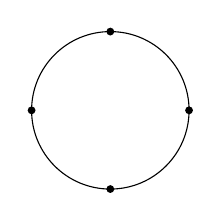
\begin{tikzpicture}
\draw circle(1)
      foreach\s in{1,...,4}{
          (-360/4*\s:-1)node[fill,circle, inner sep=1pt, name=node\s]{}
      };
\end{tikzpicture}
\end{subfigure}
\begin{subfigure}{0.15\linewidth}
\centering
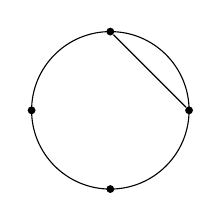
\begin{tikzpicture}
\draw circle(1)
      foreach\s in{1,...,4}{
          (-360/4*\s:-1)node[fill,circle, inner sep=1pt, name=node\s]{}
      };
\draw[-] (node1) -- (node2);
\end{tikzpicture}
\end{subfigure}
\begin{subfigure}{0.15\linewidth}
\centering
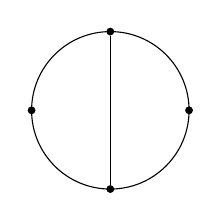
\begin{tikzpicture}
\draw circle(1)
      foreach\s in{1,...,4}{
          (-360/4*\s:-1)node[fill,circle, inner sep=1pt, name=node\s]{}
      };
\draw[-] (node1) -- (node3);
\end{tikzpicture}
\end{subfigure}\\
\begin{subfigure}{0.15\linewidth}
\centering
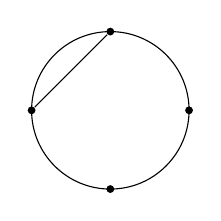
\begin{tikzpicture}
\draw circle(1)
      foreach\s in{1,...,4}{
          (-360/4*\s:-1)node[fill,circle, inner sep=1pt, name=node\s]{}
      };
\draw[-] (node1) -- (node4);
\end{tikzpicture}
\end{subfigure}
\begin{subfigure}{0.15\linewidth}
\centering
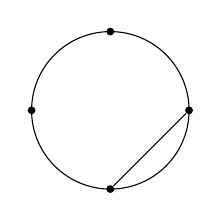
\begin{tikzpicture}
\draw circle(1)
      foreach\s in{1,...,4}{
          (-360/4*\s:-1)node[fill,circle, inner sep=1pt, name=node\s]{}
      };
\draw[-] (node2) -- (node3);
\end{tikzpicture}
\end{subfigure}
\begin{subfigure}{0.15\linewidth}
\centering
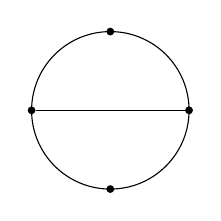
\begin{tikzpicture}
\draw circle(1)
      foreach\s in{1,...,4}{
          (-360/4*\s:-1)node[fill,circle, inner sep=1pt, name=node\s]{}
      };
\draw[-] (node2) -- (node4);
\end{tikzpicture}
\end{subfigure}\\
\begin{subfigure}{0.15\linewidth}
\centering
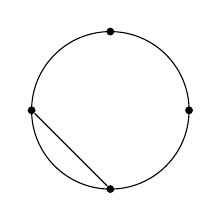
\begin{tikzpicture}
\draw circle(1)
      foreach\s in{1,...,4}{
          (-360/4*\s:-1)node[fill,circle, inner sep=1pt, name=node\s]{}
      };
\draw[-] (node3) -- (node4);
\end{tikzpicture}
\end{subfigure}
\begin{subfigure}{0.15\linewidth}
\centering
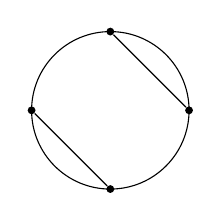
\begin{tikzpicture}
\draw circle(1)
      foreach\s in{1,...,4}{
          (-360/4*\s:-1)node[fill,circle, inner sep=1pt, name=node\s]{}
      };
\draw[-] (node1) -- (node2);
\draw[-] (node3) -- (node4);
\end{tikzpicture}
\end{subfigure}
\begin{subfigure}{0.15\linewidth}
\centering
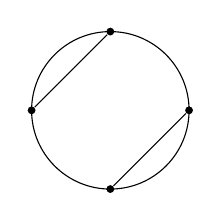
\begin{tikzpicture}
\draw circle(1)
      foreach\s in{1,...,4}{
          (-360/4*\s:-1)node[fill,circle, inner sep=1pt, name=node\s]{}
      };
\draw[-] (node1) -- (node4);
\draw[-] (node2) -- (node3);
\end{tikzpicture}
\end{subfigure}
\end{figure}

\begin{hl}
\begin{proof}
We form a bijection from the circle representation to the string representation. Identify a vertex of the circle to be the starting vertex. If it is part of a chord, begin the string with $x$. Otherwise, begin the string with $N$. Now, proceed clockwise. To the string, add an $N$ for each vertex not belonging to a chord, and add either an $x$ or $y$ otherwise. Add an $x$ if the chord has been visited already, and a $y$ otherwise. The string will be legal since each chord will cause both an $x$ and a $y$ to be added to the string, with the $x$ preceding the $y$.

\medskip

For the reverse, label the vertices in clockwise order with the integers in $[n]$. From the string, representing each $x$ by a $($, each $y$ by $)$, and removing each $N$ yields a legal string of parentheses. Identify corresponding $x$ and $y$ by identifying corresponding parentheses. Draw chords between the indices of the corresponding $x$ and $y$. The nested structure of the parentheses (and thus the $x$ and $y$) ensures that no chords will intersect.
\end{proof}
\end{hl}
\end{proposition}

\begin{proposition}\label{motzkin_recur}
$m_0=1$ and $\displaystyle m_n=m_{n-1}+\sum_{k=2}^nm_{k-2}m_{n-k}$

\begin{hl}
\begin{proof}
First, we use the string representation. Let $T\in M([n])$. Then $T$ is either of the form $T=NT'$ or $T=xT''yT'''$, where $T',T'',T'''$ are legal strings. The first case has $m_{n-1}$ elements. For the second case, condition on the position $k\neq2$ of $y$.  Then $T''\in M([k-2])$ and $T'''\in M([n-k])$, so that there are $m_{k-2}m_{n-k}$ elements.

\medskip

We can also use the chord representation. Label the vertices in clockwise order with the integers in $[n]$. If vertex 1 has no chord attached, then it can be removed to yield a chord representation on $n-1$ vertices. Otherwise, merge the vertex with its opposing vertex $k\geq 2$ at the other side of the chord to obtain a figure-8, then split this into two circles. This will yield a circle with $k-2$ vertices and one with $n-k$ vertices. Sum over all $k$.
\end{proof}
\end{hl}
\end{proposition}

\begin{proposition}\label{plomotzkin_func_eq}
The generating function for the Motzkin numbers satisfies $M(x)=1+xM(x)+x^2M(x)^2$.

\begin{hl}
\begin{proof}
Using Proposition \ref{motzkin_recur}, we have that the ordinary generating function for $m_n$ satisfies:
\begin{align*}
M(x)
&=1+\sum_{n=1}^\infty\left(m_{n-1}+\sum_{k=2}^nm_{k-2}m_{n-k}\right)x^n
=1+\sum_{n=1}^\infty m_{n-1}x^n+\sum_{n=1}^\infty\sum_{k=2}^nm_{k-2}m_{n-k}x^n\\
&=1+xM(x)+\sum_{k=2}^\infty m_{k-2}\sum_{n=k}^\infty m_{n-k}x^n
=1+xM(x)+\sum_{k=2}^\infty m_{k-2}x^k\sum_{n=0}^\infty m_{n}x^n\\
&=1+xM(x)+x^2M(x)^2\qedhere
\end{align*}
\end{proof}
\end{hl}
\end{proposition}

\begin{proposition}
$\displaystyle M_n=\frac1{n+1}\sum_{k=0}^{n+1}\binom{n+1}k\binom{n-k+1}{k-1}$

\begin{hl}
\begin{proof}
We will use Lagrange Inversion. Multiply each side of Proposition \ref{plomotzkin_func_eq} by $x$ to obtain $xM(x)=x(1+xM(x)+x^2M(x)^2)$, then let $z(x)=xM(x)$ so that $z(x)=x\phi(z)$ with $\phi(z)=1+z+z^2$. Thus:
\begin{align*}
[x^n]M(x)
&=[x^{n+1}]z(x)
=\frac1{n+1}[z^n]\phi(z)^{n+1}
=\frac1{n+1}[z^n]\sum_{k=0}^{n+1}\binom{n+1}k(z+z^2)^{n-k+1}\\
&=\frac1{n+1}\sum_{k=0}^{n+1}\binom{n+1}k[z^n]z^{n-k+1}(1+z)^{n-k+1}
=\frac1{n+1}\sum_{k=0}^{n+1}\binom{n+1}k[z^{k-1}](1+z)^{n-k+1}\\
&=\frac1{n+1}\sum_{k=0}^{n+1}\binom{n+1}k\binom{n-k+1}{k-1}\qedhere
\end{align*}
\end{proof}
\end{hl}
\end{proposition}

\begin{concept}
It can be of interest to group the elements of $M([n])$ by the number of entries that are $N$. Calling this number $k$, we can form a table with columns $k$ and rows $n$. When $k=0$ and $n$ is even, we obtain the Catalan number $c_{n/2}$.
\end{concept}

\begin{lemma}
$\displaystyle m_n=\sum_{k=0}^{\lceil n/2\rceil}\binom n{2k}c_k$

\begin{hl}
\begin{proof}
Condition on the number of letters $2k$ in the string that are not $N$. Choose their locations in the string $\binom n{2k}$ ways, and pick whether they are $x$ or $y$ by picking a legal string counted by $c_k$.
\end{proof}
\end{hl}
\end{lemma}

\begin{lemma}
$\displaystyle c_{n+1}=\sum_{k=0}^n\binom nkm_k$

\begin{hl}
\begin{proof}
Let $a_n$ count the number of ways to write a string of length $n$ over the alphabet $\{X,Y,N,M\}$ such that the tallies for $X$ always are at least the tallies for $Y$ (counting left to right) and the number of $X$ equals the number of $Y$. Such a string is called legal. We claim that $c_{n+1}=a_n$, which we show by forming a bijection as follows. To convert a legal string of $2n+2$ letters in $\{x,y\}$ to a legal string of $n$ letters over $\{X,Y,N,M\}$, remove the leading $x$ and the trailing $y$ from the string, group the remaining $2n$ letters into $n$ pairs, and make the replacements $xx\rightarrow X$, $yy\rightarrow Y$, $xy\rightarrow N$, and $yx\rightarrow M$. The inverse then makes the opposite replacements and adds a leading $x$ and a trailing $y$.

\medskip

Should the map be well-defined, it is clearly a bijection. However, we must show that the forward and inverse directions yield legal strings. It is clear that the requirement of an equal number of $x$ and $y$ (and an equal number of $X$ and $Y$) are satisfied, so it remains to show that the tally requirements are satisfied. When tallying the first $i$ letters in the string, let $t_{\alpha,i}$ denote the tally for symbol $\alpha$. We claim that for two corresponding strings, $t_{x,i}\geq t_{y,i}$ for all $i$ if and only if $t_{X,i}\geq t_{Y,i}$ for all $i$.

\medskip

By definition of the map, $t_{x,2i+1}=1+2t_{X,i}+t_{N,i}+t_{M,i}$ and $t_{y,2i+1}=2t_{Y,i}+t_{N,i}+t_{M,i}$. Hence, $t_{x,2i+1}-t_{y,2i+1}=1+2(t_{X,i}-t_{Y,i})$. This shows that $t_{x,2i+1}\geq t_{y,2i+1}$ if and only if $t_{X,i}\geq t_{Y,i}$. Furthermore, $t_{x,2i+1}-t_{y,2i+1}$ must be odd and thus at least 1. $t_{\alpha,i}$ viewed as a sequence in $i$ can only change by at most $1$ each time $i$ is incremented, so that assuming $t_{x,2i+1}-t_{y,2i+1}\geq1$ for all $i$, we have $t_{x,2i}-t_{y,2i}\geq0$ for all $i$. Altogether, we have $t_{x,i}\geq t_{y,i}$ for all $i$ if and only if $t_{X,i}\geq t_{Y,i}$ for all $i$. Hence, the bijection takes legal strings in one alphabet to legal strings in the other.

\medskip

We have thus shown that $c_{n+1}=a_n$. It remains to show $a_n=\sum_{k=0}^n\binom nkm_k$. For a string counted by $a_n$, condition on the number of letters $k$ that are not $M$. The $n-k$ letters that are $M$ can appear in any location in the string without restriction, and thus can be picked $\binom n{n-k}=\binom nk$ ways. The remaining letters $k$ can be viewed as a legal string as defined by the Motzkin numbers, so that there are $m_k$ ways to pick these. We therefore have the result.
\end{proof}
\end{hl}
\end{lemma}

\section{Posets}

\subsection{Introduction}

\begin{definition}
A \emph{poset} is a pair $(P,\leq)$ where $P$ is a set and $\leq$ is a binary relation on $P$. The relation must be reflexive ($a\leq a$), anti-symmetric ($a\leq b$ and $b\leq a$ implies $a=b$), and transitive ($a\leq b$ and $b\leq c$ implies $a\leq c$). It need not be strongly connected (there can exist two elements where neither $a\leq b$ or $b\leq a$).
\begin{arrows}
\item We use $a<b$ to mean $a\leq b$ and $a\neq b$
\end{arrows}
\end{definition}

\begin{definition}
$x\in P$ is a \emph{maximal} element of $P$ if there does not exist a $y$ with $x<y$. If $z\leq x$ for all $z\in P$, then $x$ is the \emph{maximum} element of $P$. Similar definitions hold for \emph{minimal} and \emph{minimum} elements.
\begin{arrows}
\item Every finite poset has a maximal and minimal element, but does not necessarily have a maximum or minimum element.
\item If they exist, the maximum element is denoted with $\hat 1$, and the minimum element is denoted $\hat 0$.
\end{arrows}
\end{definition}

\begin{definition}
Suppose $s,t\in P$ are elements in a poset. Then $t$ \emph{covers} $s$ (or $s$ is covered by $t$) if $s<t$ and no element $u\in P$ satisfies $s<u<t$. This is denoted by $s\lessdot t$.
\end{definition}

\begin{definition}
We denote the closed interval $[s,t]=\{u\in P\mid s\leq u\leq t\}$. Using this, $t$ covers $s$ if $[s,t]=\{s,t\}$. $[s,s]=\{s\}$ and the empty set is not considered an interval.
\end{definition}

\begin{definition}
Two posets $P$ and $Q$ are \emph{isomorphic} ($P\cong Q$) if there exists an order-preserving bijection $\phi:P\rightarrow Q$, so that $s\leq_P t$ if and only if $\phi(s)\leq_Q\phi(t)$.
\end{definition}

\begin{definition}
A poset can be represented using a \emph{Hasse diagram}. The nodes of the diagram represent each $x\in P$, and edges are drawn between nodes to represent covering relations. For each $x\lessdot y$, we must have that $x$ is vertically below $y$ and an edge connects $x$ and $y$.
\begin{arrows}
\item By transitivity, $x<y$ iff $x$ and vertically below $y$ and there is a path of edges from $x$ to $y$.
\end{arrows}
\end{definition}

\begin{definition}
A \emph{chain} is a poset (or subset of a poset) in which any two elements are comparable. If no elements in a subset of a poset are comparable, it is called an \emph{antichain}. A chain or antichain is \emph{maximal} if no further element can be added to it without breaking the chain/antichain property. It is \emph{maximum} if $P$ has no longer chain or antichain.
\end{definition}

\begin{example}
Consider a chain of length $n$ given by $C_n=\{0,1,\dots,n\}$ with partial order defined as normal in $\Z$. The Hasse diagram is:

\begin{figure}[H]
\centering
% https://tikzcd.yichuanshen.de/#N4Igdg9gJgpgziAXAbVABwnAlgFyxMJZABgBpiBdUkANwEMAbAVxiXBAF9T1Nd9CUZAIxVajFmwA6kmlAg4EXHtjwEiZAEyj6zVohBDO3EBhX91pAMzbxekMU6iYUAObwioAGYAnCAFskMhAcCCQhagALGDooNkgwViUQH38w6hCkDUjo2P14xOMUgMQs4NDES2yYuIJEig4gA
\begin{tikzcd}
n \arrow[d, no head]      \\
\vdots \arrow[d, no head] \\
1 \arrow[d, no head]      \\
0
\end{tikzcd}
\end{figure}
\end{example}

\begin{example}
The \emph{Boolean Algebra} $(B_n,\subset)$ where $B_n=\mathcal P([n])$ is a poset. The Hasse diagram for $B_3$ is as follows. Note that not all elements are comparable.

\begin{figure}[H]
\centering
% https://tikzcd.yichuanshen.de/#N4Igdg9gJgpgziAXAbVABwnAlgFyxMJZARgBoAGAXVJADcBDAGwFcYkQAdD4MgJlIDMXAL4hhpdJlz5CKcqWLU6TVuy49SvEWIkgM2PASJlFNBizaJO3MkI6jxkgzKL9Tyi2u787D3fukjOU0lc1UrdWJtRz0pQ1kSELMVS2tgLXsdJ0CE-l5QlK9gXyzY5yDEgQLPCI4GACdIHAALLDAAczElGCh2+CJQADN6iABbJHkQHAgkMhBmmHoodkgwNhjhsYmaaaQBGgWllYJ13U3xxEndxH55xeWrVdOhkYu564AWA-vjtdLz2Y7GaIACs3yOjxO-1eSFun3BD3AUI2MJuQKQADYEb9niAAYh9lNgWC7hCkX8UVsCejEFjSYintCqV8iUgAOw0Rj0ABGMEYAAU4i4rIwYIMcCBsZCKWdUSTrhyQFzeQKhUElWKJVLybj8XSFdrGcJKMIgA
\begin{tikzcd}[column sep=1.5em]
& {\{1,2,3\}} \arrow[ld, no head] \arrow[rd, no head] \arrow[d, no head] &                                                  \\
{\{1,2\}} \arrow[d, no head] \arrow[rd, no head] & {\{1,3\}} \arrow[ld, no head] \arrow[rd, no head]                      & {\{2,3\}} \arrow[ld, no head] \arrow[d, no head] \\
\{1\} \arrow[rd, no head]                        & \{2\} \arrow[d, no head]                                               & \{3\} \arrow[ld, no head]                        \\
& \varnothing                                                            &
\end{tikzcd}
\end{figure}
\end{example}

\begin{example}
The \emph{Divisor Lattice} $(D_n,|)$ consists of all positive integers $k$ that divide $n$. Example Hasse diagrams include:
\begin{figure}[H]
\centering
\begin{subfigure}{0.48\linewidth}
\centering
% https://tikzcd.yichuanshen.de/#N4Igdg9gJgpgziAXAbVABwnAlgFyxMJZAJgBoAGAXVJADcBDAGwFcYkQBGADhAF9T0mXPkIoAzKQ7U6TVuwCcfASAzY8BIh0nSGLNohAA2JYLUiiZYjtn6QYkyqHrRycqSs1dcg8QerhGihaYtZ67Bx80jBQAObwRKAAZgBOEAC2SG4gOBBIZCAAFjD0UOyQYGz8SakZiPk5SAAsNEUlZQSVyinpmTQNiFqFxaUG5Z3VPXV9uYgSQ22jHQ7dtYP9c60j4EtVICtN00gArC3D7RXLNUhz-SfzW2ORvEA
\begin{tikzcd}[column sep=1.5em]
                      &                                           & 18 \arrow[ld, no head] \arrow[rd, no head] &                       \\
                      & 6 \arrow[ld, no head] \arrow[rd, no head] &                                            & 9 \arrow[ld, no head] \\
2 \arrow[rd, no head] &                                           & 3 \arrow[ld, no head]                      &                       \\
                      & 1                                         &                                            &
\end{tikzcd}
\caption*{$D_{18}$}
\end{subfigure}
\begin{subfigure}{0.48\linewidth}
% https://tikzcd.yichuanshen.de/#N4Igdg9gJgpgziAXAbVABwnAlgFyxMJZARgBpiBdUkANwEMAbAVxiRAGYAGEAX1PUy58hFJ1IAmKrUYs2xAKy9+IDNjwEi7clPrNWiEOO58Ba4UXnbqu2QeLilpoRpTjSnHTP0gAbMeWqziLIbpLWXnL+TurBZOyeemyKJiqCMUQALBIJtr6OqWYuyFrx4YkG7PmB6ShZGTnexFVp5iiWpdLlhs2FwT7ZZbkZvFIwUADm8ESgAGYAThAAtkhZIDgQSGIgABYwdFBskGCsKfNLK9TrSG47ewcGRyfKZ8uIW1eIZLf7hwRPswtXjcPpYQAw6AAjGAMAAKLRcYJgMxwIGoux+Dz++ReSC+H3633u4Cxp0Bm0uG0QoPRRMe2LJVIpSAJNN+x3p50Qqw+WkJbP+IBxbyZiAA7Gi7vyOa88ZSABwSjHE9mkzm8j7ivmYlXPBmaj4KrXKgVCw0fACcitpJN1nP1lOIW1Z2pNDPVDq+zuN0txstxTslLp9n3elMtRrpqteoI+jqtUqjzJF4a9kdtQJFxE9ge9PAoPCAA
\begin{tikzcd}[column sep=1.5em]
                                             &                                                                  & 60 \arrow[ld, no head] \arrow[rd, no head] \arrow[rrrd, no head] &                                              &                                           &                                            &                       \\
                                             & 30 \arrow[ld, no head] \arrow[rd, no head] \arrow[rrrd, no head] &                                                                  & 20 \arrow[ld, no head] \arrow[rrrd, no head] &                                           & 12 \arrow[ld, no head] \arrow[rd, no head] &                       \\
15 \arrow[rd, no head] \arrow[rrrd, no head] &                                                                  & 10 \arrow[ld, no head] \arrow[rrrd, no head]                     &                                              & 6 \arrow[ld, no head] \arrow[rd, no head] &                                            & 4 \arrow[ld, no head] \\
                                             & 5 \arrow[rrrd, no head]                                          &                                                                  & 3 \arrow[rd, no head]                        &                                           & 2 \arrow[ld, no head]                      &                       \\
                                             &                                                                  &                                                                  &                                              & 1                                         &                                            &
\end{tikzcd}
\caption*{$D_{60}$}
\end{subfigure}
\end{figure}
\end{example}

\begin{example}
The \emph{lattice of partitions} $(\Pi_n,\leq)$ is the set of all set partitions of $[n]$. For two partitions $\gamma,\delta\in\Pi_n$, $\gamma\leq\delta$ if every block of $\gamma$ is contained in some block of $\delta$, so that $\gamma$ is a refinement of $\delta$. The Hasse diagram for $\Pi_3$ is:
\begin{figure}[H]
\centering
% https://tikzcd.yichuanshen.de/#N4Igdg9gJgpgziAXAbVABwnAlgFyxMJZARgBoAGAXVJADcBDAGwFcYkRiAmAZhAF9S6TLnyEU5UsWp0mrdlwD0vAUOx4CRMlJoMWbRB24LO-QSAxrRRTpOm65B4seVmLIjSjKc7s-R2NK-NIwUADm8ESgAGYAThAAtkgSIDgQSGQgABYw9FDskGBsKiCxCUk0qUg2WTl5BgVFZqWJiMmViNw02bn5BI3RcS0Z7QAsXbW9haYDZYjVo+M99X3TJYNInSlpiGM1S+ArfJR8QA
\begin{tikzcd}[column sep=1.5em]
                         & 123 \arrow[ld, no head] \arrow[d, no head] \arrow[rd, no head] &                          \\
12/3 \arrow[rd, no head] & 13/2 \arrow[d, no head]                                        & 1/23 \arrow[ld, no head] \\
                         & 1/2/3                                                          &
\end{tikzcd}
\end{figure}
\end{example}

\begin{example}
The \emph{lattice of compositions} $(K_n,\leq)$ is the set of all compositions of $n$ with order defined by the refinement of compositions. The Hasse diagram for $K_4$ is:
\begin{figure}[H]
\centering
% https://tikzcd.yichuanshen.de/#N4Igdg9gJgpgziAXAbVABwnAlgFyxMJZARgBoBmAXVJADcBDAGwFcYkRiBqLnkAX1LpMufIRQAGUgCZqdJq3ZTu3foJAZseAkTIyaDFm0QdOS4qqGbRRKdNkGFxnqYvrhWscknF78oyHIVAUsRbRQyH30-RRdgtysw5FtIuUN2LnJXDVDPMnFfNOMAFn5ZGCgAc3giUAAzACcIAFskMhAcCCRJEAALGHoodkgwNjiG5qRbds7Ebr6BoYJRtXGWxHIaDq6aecHjYeW6xrWizZm23cWR11WkU+nJnf698CWb46QAVjPWp4X9t5jD6Ib4PdZ-F4Hd4TRAANh+iCmlwB1yBMPhYI2vWeV0OIFuiAA7AjQcjXqiVsD7lsiRDcdC1sSwRiyVC+JQ+EA
\begin{tikzcd}[column sep={6em,between origins}]
                                                               & 4 \arrow[d, no head] \arrow[rd, no head]    &                                            \\
3+1 \arrow[d, no head] \arrow[rd, no head] \arrow[ru, no head] & 2+2 \arrow[ld, no head] \arrow[rd, no head] & 1+3 \arrow[ld, no head] \arrow[d, no head] \\
2+1+1 \arrow[rd, no head]                                      & 1+2+1 \arrow[d, no head]                    & 1+1+2 \arrow[ld, no head]                  \\
                                                               & 1+1+1+1                                     &
\end{tikzcd}
\end{figure}
\end{example}

\begin{example}
The \emph{Young lattice} $(Y,\leq)$ is the set of all integer partitions and $\alpha\leq\beta$ if the Young diagram for $\alpha$ is contained in the Young diagram for $\beta$. The Hasse diagram for $Y$ up to integer partitions of 4 is:
\begin{figure}[H]
\centering
% https://tikzcd.yichuanshen.de/#N4Igdg9gJgpgziAXAbVABwnAlgFyxMJZAZgBpiBdUkANwEMAbAVxiRAAoBGAShAF9S6TLnyEUAJlLiqtRizbtxvAUOx4CRACxSZ9Zq0QdOpHv0EgMa0UWOddcgx2LLzlkRpRk71PfMOKTF1V3MWQAVhN7fQVbQLNg9VCyAAYovw5JJXiLYUStUlSfBwVJWyCcqw9kADYCtMcuEybTFQqQoklC2Wj-L3K3PJRkuqKejk1lGRgoAHN4IlAAMwAnCABbJGMQHAgkYZAACxg6KDZIMFZWlfWkSW3dxH2jk7OCS-NrjcQye83qZ9OhnO7yWqy+2l+iC2ANeF2ynyQEJ2t3+x0B4De8LBSAikLuMKBmKu2MQAA5qMjELiCRi4cSbogAOwUh7UtGwkEgBFMlmI1EvQl0j4k2qQiE04FYhkATl5iHF7MFnO5sshPwlROFDM4+0p6sVtMuFD4QA
\begin{tikzcd}[column sep={4em,between origins}]
\begin{array}{c}(4)\\\scalebox{0.5}{\ydiagram{4}}\end{array} \arrow[rd, no head] & & \begin{array}{c}(3,1)\\\scalebox{0.5}{\ydiagram{3,1}}\end{array} \arrow[rd, no head] \arrow[ld, no head] &  \begin{array}{c}(2,2)\\\scalebox{0.5}{\ydiagram{2,2}}\end{array} \arrow[d, no head] &  \begin{array}{c}(2,1,1)\\\scalebox{0.5}{\ydiagram{2,1,1}}\end{array} \arrow[rd, no head] \arrow[ld, no head] & &  \begin{array}{c}(1,1,1,1)\\\scalebox{0.5}{\ydiagram{1,1,1,1}}\end{array} \arrow[ld, no head] \\
 &  \begin{array}{c}(3)\\\scalebox{0.5}{\ydiagram{3}}\end{array} \arrow[rd, no head] & & \begin{array}{c}(2,1)\\\scalebox{0.5}{\ydiagram{2,1}}\end{array} \arrow[ld, no head] \arrow[rd, no head] & & \begin{array}{c}(1,1,1)\\\scalebox{0.5}{\ydiagram{1,1,1}}\end{array} \arrow[ld, no head] & \\
 & & \begin{array}{c}(2)\\\scalebox{0.5}{\ydiagram{2}}\end{array} \arrow[rd, no head] & & \begin{array}{c}(1,1)\\\scalebox{0.5}{\ydiagram{1,1}}\end{array} \arrow[ld, no head] & & \\
 & & & \begin{array}{c}(1)\\\scalebox{0.5}{\ydiagram{1}}\end{array} & & &
\end{tikzcd}
\end{figure}
\end{example}

\begin{concept}\label{poset_arbitrary}
We can the Hasse diagrams for isomorphism classes of posets of a given size. We have:
\begin{table}[H]
\centering
\begin{tabular}{c|c|c}
Size 1&Size 2&Size 3\\

\begin{tikzpicture}[x=0.4cm, y=0.4cm]
\node[circle, draw, fill=black, inner sep=2pt] (0) at (0, 0) {};
\end{tikzpicture}
&
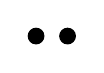
\begin{tikzpicture}[x=0.4cm, y=0.4cm]
    \node[circle, draw, fill=black, inner sep=2pt] (0) at (0, 0) {};
    \node[circle, draw, fill=black, inner sep=2pt] (1) at (1, 0) {};
\end{tikzpicture}\qquad
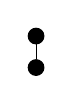
\begin{tikzpicture}[x=0.4cm, y=0.4cm]
    \node[circle, draw, fill=black, inner sep=2pt] (0) at (0, 1) {};
    \node[circle, draw, fill=black, inner sep=2pt] (1) at (0, 0) {};
    \draw (0) -- (1);
\end{tikzpicture}
&
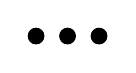
\begin{tikzpicture}[x=0.4cm, y=0.4cm]
    \node[circle, draw, fill=black, inner sep=2pt] (0) at (0, 0) {};
    \node[circle, draw, fill=black, inner sep=2pt] (1) at (1, 0) {};    \node[circle, draw, fill=black, inner sep=2pt] (2) at (2, 0) {};
\end{tikzpicture}\qquad
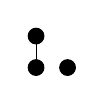
\begin{tikzpicture}[x=0.4cm, y=0.4cm]
    \node[circle, draw, fill=black, inner sep=2pt] (0) at (0, 0) {};
    \node[circle, draw, fill=black, inner sep=2pt] (1) at (0, 1) {};    \node[circle, draw, fill=black, inner sep=2pt] (2) at (1, 0) {};
    \draw (0) -- (1);
\end{tikzpicture}\qquad
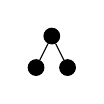
\begin{tikzpicture}[x=0.4cm, y=0.4cm]
    \node[circle, draw, fill=black, inner sep=2pt] (0) at (0, 0) {};
    \node[circle, draw, fill=black, inner sep=2pt] (1) at (0.5, 1) {};    \node[circle, draw, fill=black, inner sep=2pt] (2) at (1, 0) {};
    \draw (0) -- (1) -- (2);
\end{tikzpicture}\qquad

\begin{tikzpicture}[x=0.4cm, y=0.4cm]
    \node[circle, draw, fill=black, inner sep=2pt] (0) at (0, 1) {};
    \node[circle, draw, fill=black, inner sep=2pt] (1) at (0.5, 0) {};    \node[circle, draw, fill=black, inner sep=2pt] (2) at (1, 1) {};
    \draw (0) -- (1) -- (2);
\end{tikzpicture}\qquad
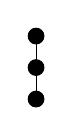
\begin{tikzpicture}[x=0.4cm, y=0.4cm]
    \node[circle, draw, fill=black, inner sep=2pt] (0) at (0, 0) {};
    \node[circle, draw, fill=black, inner sep=2pt] (1) at (0, 1) {};    \node[circle, draw, fill=black, inner sep=2pt] (2) at (0, 2) {};
    \draw (0) -- (1) -- (2);
\end{tikzpicture}
\end{tabular}
\end{table}
\end{concept}

\begin{example}
The posets of size 4 are:
\begin{figure}[H]
\centering
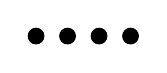
\begin{tikzpicture}[x=0.4cm, y=0.4cm]
    \node[circle, draw, fill=black, inner sep=2pt] (0) at (0, 0) {};
    \node[circle, draw, fill=black, inner sep=2pt] (1) at (1, 0) {};    \node[circle, draw, fill=black, inner sep=2pt] (2) at (2, 0) {};
	\node[circle, draw, fill=black, inner sep=2pt] (3) at (3, 0) {};
\end{tikzpicture}\qquad
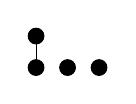
\begin{tikzpicture}[x=0.4cm, y=0.4cm]
    \node[circle, draw, fill=black, inner sep=2pt] (0) at (0, 0) {};
    \node[circle, draw, fill=black, inner sep=2pt] (1) at (0, 1) {};    \node[circle, draw, fill=black, inner sep=2pt] (2) at (1, 0) {};
	\node[circle, draw, fill=black, inner sep=2pt] (3) at (2, 0) {};
	\draw (0) -- (1);
\end{tikzpicture}\qquad
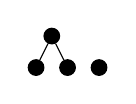
\begin{tikzpicture}[x=0.4cm, y=0.4cm]
    \node[circle, draw, fill=black, inner sep=2pt] (0) at (0, 0) {};
    \node[circle, draw, fill=black, inner sep=2pt] (1) at (0.5, 1) {};    \node[circle, draw, fill=black, inner sep=2pt] (2) at (1, 0) {};
	\node[circle, draw, fill=black, inner sep=2pt] (3) at (2, 0) {};
	\draw (0) -- (1) -- (2);
\end{tikzpicture}\qquad
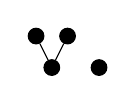
\begin{tikzpicture}[x=0.4cm, y=0.4cm]
    \node[circle, draw, fill=black, inner sep=2pt] (0) at (0, 1) {};
    \node[circle, draw, fill=black, inner sep=2pt] (1) at (0.5, 0) {};    \node[circle, draw, fill=black, inner sep=2pt] (2) at (1, 1) {};
	\node[circle, draw, fill=black, inner sep=2pt] (3) at (2, 0) {};
	\draw (0) -- (1) -- (2);
\end{tikzpicture}\qquad
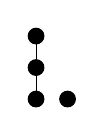
\begin{tikzpicture}[x=0.4cm, y=0.4cm]
    \node[circle, draw, fill=black, inner sep=2pt] (0) at (0, 0) {};
    \node[circle, draw, fill=black, inner sep=2pt] (1) at (0, 1) {};    \node[circle, draw, fill=black, inner sep=2pt] (2) at (0, 2) {};
	\node[circle, draw, fill=black, inner sep=2pt] (3) at (1, 0) {};
	\draw (0) -- (1) -- (2);
\end{tikzpicture}\qquad
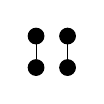
\begin{tikzpicture}[x=0.4cm, y=0.4cm]
    \node[circle, draw, fill=black, inner sep=2pt] (0) at (0, 0) {};
    \node[circle, draw, fill=black, inner sep=2pt] (1) at (0, 1) {};    \node[circle, draw, fill=black, inner sep=2pt] (2) at (1, 0) {};
	\node[circle, draw, fill=black, inner sep=2pt] (3) at (1, 1) {};
	\draw (0) -- (1);
	\draw (2) -- (3);
\end{tikzpicture}\qquad
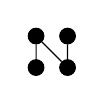
\begin{tikzpicture}[x=0.4cm, y=0.4cm]
    \node[circle, draw, fill=black, inner sep=2pt] (0) at (0, 0) {};
    \node[circle, draw, fill=black, inner sep=2pt] (1) at (0, 1) {};    \node[circle, draw, fill=black, inner sep=2pt] (2) at (1, 0) {};
	\node[circle, draw, fill=black, inner sep=2pt] (3) at (1, 1) {};
	\draw (0) -- (1) -- (2) -- (3);
\end{tikzpicture}\qquad
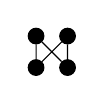
\begin{tikzpicture}[x=0.4cm, y=0.4cm]
    \node[circle, draw, fill=black, inner sep=2pt] (0) at (0, 0) {};
    \node[circle, draw, fill=black, inner sep=2pt] (1) at (0, 1) {};    \node[circle, draw, fill=black, inner sep=2pt] (2) at (1, 0) {};
	\node[circle, draw, fill=black, inner sep=2pt] (3) at (1, 1) {};
	\draw (0) -- (1) -- (2) -- (3) -- (0);
\end{tikzpicture}\qquad
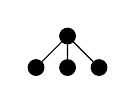
\begin{tikzpicture}[x=0.4cm, y=0.4cm]
    \node[circle, draw, fill=black, inner sep=2pt] (0) at (0, 0) {};
    \node[circle, draw, fill=black, inner sep=2pt] (1) at (1, 0) {};    \node[circle, draw, fill=black, inner sep=2pt] (2) at (2, 0) {};
	\node[circle, draw, fill=black, inner sep=2pt] (3) at (1, 1) {};
	\draw (0) -- (3) -- (1);
	\draw (3) -- (2);
\end{tikzpicture}\qquad
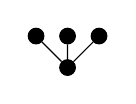
\begin{tikzpicture}[x=0.4cm, y=0.4cm]
    \node[circle, draw, fill=black, inner sep=2pt] (0) at (0, 1) {};
    \node[circle, draw, fill=black, inner sep=2pt] (1) at (1, 1) {};    \node[circle, draw, fill=black, inner sep=2pt] (2) at (2, 1) {};
	\node[circle, draw, fill=black, inner sep=2pt] (3) at (1, 0) {};
	\draw (0) -- (3) -- (1);
	\draw (3) -- (2);
\end{tikzpicture}

\medskip

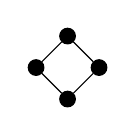
\begin{tikzpicture}[x=0.4cm, y=0.4cm]
    \node[circle, draw, fill=black, inner sep=2pt] (0) at (1, 0) {};
    \node[circle, draw, fill=black, inner sep=2pt] (1) at (0, 1) {};    \node[circle, draw, fill=black, inner sep=2pt] (2) at (2, 1) {};
	\node[circle, draw, fill=black, inner sep=2pt] (3) at (1, 2) {};
	\draw (0) -- (1) -- (3) -- (2) -- (0);
\end{tikzpicture}\qquad
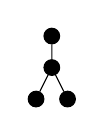
\begin{tikzpicture}[x=0.4cm, y=0.4cm]
    \node[circle, draw, fill=black, inner sep=2pt] (0) at (0, 0) {};
    \node[circle, draw, fill=black, inner sep=2pt] (1) at (0.5, 1) {};    \node[circle, draw, fill=black, inner sep=2pt] (2) at (0.5, 2) {};
	\node[circle, draw, fill=black, inner sep=2pt] (3) at (1, 0) {};
	\draw (0) -- (1) -- (2);
	\draw (1) -- (3);
\end{tikzpicture}\qquad
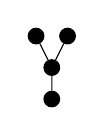
\begin{tikzpicture}[x=0.4cm, y=0.4cm]
    \node[circle, draw, fill=black, inner sep=2pt] (0) at (0, 2) {};
    \node[circle, draw, fill=black, inner sep=2pt] (1) at (0.5, 1) {};    \node[circle, draw, fill=black, inner sep=2pt] (2) at (0.5, 0) {};
	\node[circle, draw, fill=black, inner sep=2pt] (3) at (1, 2) {};
	\draw (0) -- (1) -- (2);
	\draw (1) -- (3);
\end{tikzpicture}\qquad
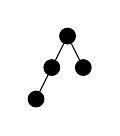
\begin{tikzpicture}[x=0.4cm, y=0.4cm]
    \node[circle, draw, fill=black, inner sep=2pt] (0) at (0, 0) {};
    \node[circle, draw, fill=black, inner sep=2pt] (1) at (0.5, 1) {};    \node[circle, draw, fill=black, inner sep=2pt] (2) at (1, 2) {};
	\node[circle, draw, fill=black, inner sep=2pt] (3) at (1.5, 1) {};
	\draw (0) -- (1) -- (2) -- (3);
\end{tikzpicture}\qquad
\begin{tikzpicture}[x=0.4cm, y=0.4cm]
    \node[circle, draw, fill=black, inner sep=2pt] (0) at (0, 2) {};
    \node[circle, draw, fill=black, inner sep=2pt] (1) at (0.5, 1) {};    \node[circle, draw, fill=black, inner sep=2pt] (2) at (1, 0) {};
	\node[circle, draw, fill=black, inner sep=2pt] (3) at (1.5, 1) {};
	\draw (0) -- (1) -- (2) -- (3);
\end{tikzpicture}\qquad
\begin{tikzpicture}[x=0.4cm, y=0.4cm]
    \node[circle, draw, fill=black, inner sep=2pt] (0) at (0, 0) {};
    \node[circle, draw, fill=black, inner sep=2pt] (1) at (0, 1) {};    \node[circle, draw, fill=black, inner sep=2pt] (2) at (0, 2) {};
	\node[circle, draw, fill=black, inner sep=2pt] (3) at (0, 3) {};
	\draw (0) -- (1) -- (2) -- (3);
\end{tikzpicture}
\end{figure}
\end{example}

\begin{example}
Every finite poset $P$ is isomorphic to a subset of $B_n$ for some $n$.

\begin{hl}
\begin{proof}
Pick $n=|P|$ and label each element by a unique element in $[n]$ via a linear extension; we use the values in $[n]$ to refer to the elements of $P$. Form the isomorphism $\phi:P\rightarrow Q$ for $Q\subset B_n$ by $k\mapsto\{k\}\cup\bigcup_{j<k}\phi(j)$. We prove by induction on $k$ that if $q\in\phi(k)$, then $q\leq k$. The base case of $k=1$ is trivial since $1$ is minimal and maps to $\{1\}$. For induction, suppose $q\in\phi(k)=\{k\}\cup\bigcup_{j<k}\phi(j)$. Then either $q=k$ (which satisfies the claim) or $q\in\phi(j)$ for some $j<k$. By induction, $q\leq j<k$, so $q<k$ (which also satisfies the claim).

\medskip

We show $\phi$ is injective. If $\phi(j)=\phi(k)$, then $j\in\phi(k)$ which means $j\leq k$. Conversely, $k\in\phi(j)$ which implies $k\leq j$. Hence, $k=j$.

\medskip

Now we show $\phi$ is order-preserving. For any $j\leq k$, we have $\phi(j)\leq\phi(k)$ by definition. Furthermore, for any $j\not\leq k$, we have $j\not\in\phi(k)$ by the contrapositive of the previous claim. Since $j\in\phi(j)$, we have $\phi(j)\not\leq\phi(k)$.
\end{proof}
\end{hl}
\end{example}

\begin{definition}
A \emph{linear extension} of a poset with $n$ elements is an order-preserving bijection from $P$ onto $[n]$. That is, for bijection $f:P\rightarrow[n]$, $x\leq y$ implies $f(x)\leq f(y)$.
\begin{arrows}
\item Linear extensions allow us to code many aspects of a poset using upper triangular matrices, as we will see in later sections.
\end{arrows}
\end{definition}

\begin{example}
We describe the linear extensions of elements of the posets of size 3 (see Concept \ref{poset_arbitrary}). The first has $6=3!$ linear extensions, corresponding to any bijection from the three vertices to $[3]$. The second has 3 linear extensions. Indeed, the lone vertex can be mapped to any element in $[3]$, and then the remaining two are uniquely determined so that order is preserved. The third has 2 linear extensions, where the two non-comparable elements are mapped to $\{1,2\}$ and the maximum element is mapped to 3. The fourth also has 2 linear extensions, where the minimum element is mapped to 1 and the remaining two are mapped to $\{2,3\}$. The last is a chain, and thus has 1 linear extension.
\end{example}

\begin{example}
Consider the posets:
\begin{figure}[H]
\centering
\begin{tikzpicture}[x=0.4cm, y=0.4cm]
    \node[circle, draw, fill=black, inner sep=2pt] (0) at (0, 0) {};
    \node[circle, draw, fill=black, inner sep=2pt] (1) at (0.5, 1) {};    \node[circle, draw, fill=black, inner sep=2pt] (2) at (1, 0) {};
	\node[circle, draw, fill=black, inner sep=2pt] (3) at (2, 0) {};
	\draw (0) -- (1) -- (2);
\end{tikzpicture}\qquad
\begin{tikzpicture}[x=0.4cm, y=0.4cm]
    \node[circle, draw, fill=black, inner sep=2pt] (0) at (0, 1) {};
    \node[circle, draw, fill=black, inner sep=2pt] (1) at (0.5, 0) {};    \node[circle, draw, fill=black, inner sep=2pt] (2) at (1, 1) {};
	\node[circle, draw, fill=black, inner sep=2pt] (3) at (2, 0) {};
	\draw (0) -- (1) -- (2);
\end{tikzpicture}
\end{figure}

Each has precisely 8 linear extensions. Indeed, the element with no relations can be assigned 4 ways. After this, the maximum/minimum element of the remaining elements must map to the maximum/minimum element of the remaining elements in $[4]$. The last two elements can be mapped $2!=2$ ways.
\end{example}

\begin{definition}
A \emph{chain cover} of a poset $P$ is a collection of disjoint chains whose union is $P$. The \emph{size} of a chain cover is the number of chains in it.
\begin{arrows}
\item The chains do not need to be maximal. In other words, the relations in the chains do not need to be covering relations.
\end{arrows}
\end{definition}

\begin{theorem}[Dilworth's Theorem]
In a finite poset $P$, the size of any maximum antichain is equal to the size of the smallest chain cover.

\begin{hl}
\begin{proof}
Let $a$ be the size of a maximum antichain and $b$ be the size of any smallest chain cover. Then $a\leq b$ since each element of the antichain must belong to a separate chain in the cover. For the converse, we induct on the size $n$ of $P$. The base case $n=1$ is trivial, so assume $n>1$. There are two cases:
\begin{itemize}
\item $P$ contains an $a$-element antichain $A$ with at least one element that is not minimal and at least one element that is not maximal. Then $A$ splits $P$ into two sets: $U$ which contains all elements greater than or equal to some element of $A$, and $L$ which contains all elements less than or equal to some element of $A$. $L\cap U=A$ since otherwise we would arrive at a contradiction by transitivity. Since $A$ contains both a non-minimal and non-maximal element, $U$ and $L$ are non-empty, and so are each unions of $a$ chains by the inductive hypothesis. Each chain in $L$ has an element of $A$ at its top, and each chain in $U$ has an element of $A$ at its bottom. Join the corresponding chains to obtain a covering of $p$ by $a$ chains.
\item $P$ does not have such an antichain. Then either all elements are minimal, or all are maximal. Pick $x$ minimal and $y$ maximal with $x\leq y$. Let $P'$ be the poset with $x$ and $y$ removed. The maximal antichain of $P'$ now has $a-1$, so by induction, $P'$ can be covered with $k-1$ chains. Now add the chain $x\leq y$ to obtain that $P$ can be covered by $a$ chains.
\end{itemize}
\end{proof}
\end{hl}
\end{theorem}

\begin{example}
The number of 2-element chains in $B_n$ is $3^n-2^n$. Indeed, for $x\leq y$, there are $3^n$ ways to mark elements as either in $x$, in both $x$ and $y$, or in neither. Then we subtract the $2^n$ pairs $(x,y)$ such that $x=y$. This results means the number of 2-element antichains in $B_n$ is:
\begin{equation*}
\binom{2^n}2-(3^n-2^n)
=\frac12\cdot2^n(2^n-1)-3^n+2^n
=\frac12\cdot4^n-3^n+\frac12\cdot2^n
\end{equation*}
\end{example}

\subsection{Incidence Algebra}

\begin{definition}
A poset is called \emph{locally finite} if all closed intervals have a finite number of elements.
\begin{arrows}
\item Not all posets that are locally finite are also finite. For example, the integers are locally finite but not finite.
\end{arrows}
\end{definition}

\begin{definition}
A set of elements $I\subset P$ is called an \emph{ideal} if $x\in I$ and $y\leq x$ implies $y\in I$. In other words, an ideal is a set closed under choosing smaller elements. A \emph{principal ideal} is a ideal generated by a single elements, so that $I=\{y\mid y\leq x\}$ for some $x\in P$.
\end{definition}

\begin{concept}
In some of our later results, we require that every principal ideal of $P$ is finite. This means that each element is larger than a finite number of elements only. This is a stronger requirement then $P$ being locally finite. For example, the integers are locally finite but has no finite principal ideals.
\end{concept}

\begin{definition}
Let $P$ be a locally finite poset. The \emph{incidence algebra} $I(P)$ is the set of all functions $f:\Inte(P)\rightarrow\C$, where $\Inte(P)$ is the set of all intervals in $P$. We denote $f(x,y)=f([x,y])$ for ease of notation. Addition is defined by $(f+g)(x,y)=f(x,y)+g(x,y)$ and multiplication by $(fg)(x,y)=\sum_{x\leq z\leq y}f(x,z)g(z,y)$.

\medskip

This can be viewed through matrices for a finite poset. Indeed, consider a linear extension $x_1,\dots,x_n$ of $P$, then for $f\in I(p)$ form the $n\times n$ matrix with $ij$th entry $f(x_i,x_j)$. Here, we define $f(x_i,x_j)$ with $[x_i,x_j]\not\in\Inte(P)$. Since the linear extension respects the order in the poset, the matrix will be upper triangular with a certain pattern of zeros corresponding to non-comparable elements. The addition and multiplication operations in $I(P)$ correspond to the usual operations in the matrices. In particular, $I(P)$ is isomorphic to a subalgebra of the $n\times n$ upper triangular matrices.
\begin{arrows}
\item The proof that $\Inte(P)$ is an algebra is straight forward
\end{arrows}
\end{definition}

\begin{definition}
The multiplicative identity in $I(P)$ is $\delta(x,y)=I[x=y]$. This satisfies $\delta f=f\delta=f$, since the corresponding matrix to $\delta$ is the identity matrix.
\end{definition}

\begin{lemma}\label{ip_inv}
Let $f\in I(P)$ for a locally finite poset $P$. Then the following conditions are equivalent:
\begin{enumerate}[label=(\roman*)]
\item $f$ has a left inverse
\item $f$ has a right inverse
\item $f$ is invertible
\item $f(x,x)\neq 0$ for all $x\in P$
\end{enumerate}

\begin{hl}
\begin{proof}
(iii) implies (iv) since $fg=\delta$ implies $f(x,x)g(x,x)=1$ for all $x\in P$. (i) and (ii) together imply (iii). It remains to show that (iv) implies (i) and (ii). We construct the right inverse, and a similar technique can be used for the left inverse. We inductively define:
\begin{equation*}
g(x,x)=f(x,x)^{-1}\quad\text{and}\quad g(x,y)=-f(x,x)^{-1}\sum_{x<z\leq y}f(x,z)g(z,y)\text{ when }x\neq y
\end{equation*}

Note that each recursive computation of $g(x,y)$ decreases the size of the interval $[x,y]$, which is finite since $P$ is locally finite. Hence, the above is well-defined. It is clearly the inverse when $x=y$, and when $x\neq y$, multiplying by $f(x,x)$ and rearranging yields $\sum_{x\leq z\leq y}f(x,z)g(z,y)=0$, or $(fg)(x,y)=0=\delta(x,y)$ as desired.
\end{proof}
\end{hl}
\end{lemma}

\begin{definition}
Let $P$ be a locally finite poset. The \emph{zeta function} of $P$ is defined by $\zeta(x,y)=I[x\leq y]=1$, where $\zeta\in I(P)$.
\end{definition}

\begin{definition}\label{mobius}
Lemma \ref{ip_inv} shows that $\zeta$ is invertible. The inverse $\mu$ is called the \emph{M\"obius function} of $P$. Using the proof of Lemma \ref{ip_inv} and the fact that $\zeta(x,y)=1$ for all $[x,y]\in I(P)$, we can compute $\mu$ for $x\neq y$ as either of:
\begin{equation*}
\mu(x,y)=-\sum_{x\leq z<y}\mu(x,z)=-\sum_{x<z\leq y}\mu(z,y)
\end{equation*}
\begin{arrows}
\item An easy way of viewing this is $\sum_{x\leq z\leq y}\mu(x,y)=\delta(x,y)$. For a Hasse diagram, we can evaluate $\mu(x,y)$ by starting at $x$ and working upwards to label the value of $\mu(x,s)$ for $x\leq s\leq y$. Each value is determined by ensuring the sum of it along with the values below it sum to zero.
\end{arrows}
\end{definition}

\begin{definition}
If $P$ has a maximum and minimum element, then we denote $\mu(P)=\mu(\hat0,\hat1)$.
\end{definition}

\begin{lemma}
$\mu(x,y)$ is an integer for all $x,y\in P$.

\begin{hl}
\begin{proof}
Consider the matrix representation $Z$ of $\zeta$, which is upper triangular with diagonal elements 1. Thus, $Z^{-1}$ also has diagonal elements 1, so that the claim follows inductively by the recursive form given in Definition \ref{mobius}.

\medskip

Alternatively, note that $\det(Z)=1$, since it is upper triangular with diagonal entries 1. Hence, Cramer's rule indicates that the solutions to $Z\vec x=\vec e_i$ will be integers for any standard basis vector $\vec e_i$. Hence, $Z^{-1}$ has integer entries.
\end{proof}
\end{hl}
\end{lemma}

\begin{definition}
The M\"obius function in number theory is defined as:
\begin{equation*}
\mu(n)=\left\{
\begin{array}{ll}
+1,&\text{ if $n$ is a square-free positive integer with an even number of prime factors}\\
-1,&\text{ if $n$ is a square-free positive integer with an odd number of prime factors}\\
0,&\text{ if $n$ has a squared prime factor}
\end{array}
\right.
\end{equation*}
\end{definition}


\begin{lemma}
For a divisor lattice $P$ (or more generally the lattice of natural numbers with order given by divisibility), the two different M\"obius functions satisfy $\mu(x,y)=\mu(y/x)$ for $x|y$.
\begin{arrows}
\item As an alternative partial proof, note that when $y/x$ is a power of $k$ distinct primes, then the interval $[x,y]$ is isomorphic to the Boolean Algebra $B_k$ with $x\mapsto\varnothing$ and $y\mapsto[k]$. This gives $\mu(x,y)=\mu(\varnothing,[k])=(-1)^k$ by Lemma \ref{boolean_mobius}.
\end{arrows}

\begin{hl}
\begin{proof}
We prove this by induction on $y/x$. When $y/x=1$, the claim is trivial since $\mu(x,y)=\mu(x,x)=1=\mu(1)$. Otherwise, let the distinct prime factors of $n=y/x$ be $p_1,\dots,p_m$. By the inductive hypothesis:
\begin{align*}
\mu(x,y)
&=-\sum_{\substack{x|k|y\\k\neq y}}\mu(x,k)
=-\sum_{\substack{x|k|y\\k\neq y}}\mu(k/x)
=-\sum_{\substack{k|n\\k\neq n}}\mu(k)
=-\sum_{\substack{S\subset\{p_1,\dots,p_m\}\\\prod S\neq n}}\mu\left(\prod S\right)\\
&=-\sum_{i=0}^m \binom mi(-1)^i+I\left[\prod_{i=1}^mp_i=n\right](-1)^m
=I\left[\prod_{i=1}^mp_i=n\right](-1)^m
=\mu(n)
=\mu(y/x)
\end{align*}

Here, we used the fact that $\mu(k)$ is zero if it contains a square, so that it suffices to sum over products of distinct primes. We then used the fact that $\mu$ only depends on the number of such primes $i$. When $\prod_{i=1}^mp_i=n$, we have to add back the term corresponding to $i=m$ in the last summation, since we require $\prod S\neq n$.
\end{proof}
\end{hl}
\end{lemma}

\begin{example}
Consider the divisor lattice $D_{24}$ given below:
\begin{figure}[H]
\centering
% https://tikzcd.yichuanshen.de/#N4Igdg9gJgpgziAXAbVABwnAlgFyxMJZAZgBoAGAXVJADcBDAGwFcYkQAmAFhAF9T0mXPkIoOpAIzU6TVuwkc+AkBmx4CRCaQ7SGLNohAA2JYLUii5UsV2yDIYqZVD1o5Fq6398p6uEaxay85Q0V+M383Mh0aPRCQHnDncwDkLklg+wAOPmkYKABzeCJQADMAJwgAWyQyEBwIJHSQAAsYeih2SDA2JIrqpHF6xsQ6to6ugl7lfprELWHBmnHOw27pssq5q0X55fbV8CmnWaQdhqQAdn2JteO+raQFi8QjG8P1k8fEIZeAVnekx6XwGiGuuzerQOQI2IFOrxo-0Bd2BD1BAN2zRWMNyvCAA
\begin{tikzcd}[column sep=1.5em]
                      &                                           &                                            & 24 \arrow[ld, no head] \arrow[rd, no head] &                       \\
                      &                                           & 12 \arrow[ld, no head] \arrow[rd, no head] &                                            & 8 \arrow[ld, no head] \\
                      & 6 \arrow[ld, no head] \arrow[rd, no head] &                                            & 4 \arrow[ld, no head]                      &                       \\
3 \arrow[rd, no head] &                                           & 2 \arrow[ld, no head]                      &                                            &                       \\
                      & 1                                         &                                            &                                            &
\end{tikzcd}
\end{figure}

For any divisor lattice, the order in $\N$ provides a linear extension, so we use this here (e.g., $8\in D_{24}$ corresponds to the 6th element in the linear extension). The matrix representation of $\zeta$ is:
\begin{equation*}
\zeta\mapsto Z=\begin{pmatrix}
1&1&1&1&1&1&1&1\\
0&1&0&1&1&1&1&1\\
0&0&1&0&1&0&1&1\\
0&0&0&1&0&1&1&1\\
0&0&0&0&1&0&1&1\\
0&0&0&0&0&1&0&1\\
0&0&0&0&0&0&1&1\\
0&0&0&0&0&0&0&1
\end{pmatrix}
\end{equation*}

Inverting the matrix yields:
\begin{equation*}
\mu\mapsto M=
\begin{pmatrix}
1&-1&-1&0&1&0&0&0\\
0&1&0&-1&-1&0&1&0\\
0&0&1&0&-1&0&0&0\\
0&0&0&1&0&-1&-1&1\\
0&0&0&0&1&0&-1&0\\
0&0&0&0&0&1&0&-1\\
0&0&0&0&0&0&1&-1\\
0&0&0&0&0&0&0&1
\end{pmatrix}
\end{equation*}

Note that the first row matches what we would expect from using the number-theoretic M\"obius function. This could also have been determined using the recursive definition of $\mu$.
\end{example}

\begin{lemma}\label{boolean_mobius}
Consider the Boolean Algebra poset $B_n$ and let $S,T\in B_n$ with $T\leq S$. Then $\mu(T,S)=(-1)^{|S\setminus T|}=(-1)^{|S|-|T|}$.

\begin{hl}
\begin{proof}
We induct on $k=|S|-|T|$. $k=0$ trivially gives $\mu(T,S)=\mu(T,T)=1=(-1)^0$. Otherwise, we have:
\begin{align*}
\mu(T,S)
&=-\sum_{T\leq R<S}\mu(T,R)
=-\sum_{T\leq R<S}(-1)^{|R|-|T|}
=-\sum_{j=|T|}^{|S|-1}\binom{k}{j-|T|}(-1)^{j-|T|}\\
&=-\sum_{j=0}^{k-1}\binom{k}{j}(-1)^{j}
=-\sum_{j=0}^{k}\binom{k}{j}(-1)^{j}+\binom kk(-1)^k
=(-1)^k
=(-1)^{|S|-|T|}
\end{align*}

Here, we conditioned in $j=|R|$, then reindexed the summation.
\end{proof}
\end{hl}
\end{lemma}

\begin{lemma}\label{matrix_num_chains}
The number of chains of length $k$ that start at $x$ and end at $y$ is $(\zeta-\delta)^k(x,y)$. Using a linear extension, the number of chains of length $k$ that start at $x_i$ and end at $x_j$ is given by the entries of $(Z-I)^k$.
\begin{arrows}
\item The matrix form is analogous to a transition matrix in stochastics, where we subtract $I$ to prevent a chain from containing duplicates.
\end{arrows}

\begin{hl}
\begin{proof}
We induct on $k$. The claim is trivial when $k=1$. For $k>1$, let the chain be $x=x_1<\cdots<x_k=y$, and condition on $x_{k-1}$, which we call $z$. Form a chain of length $k-1$ from $x_1$ to $z$ $(\zeta-\delta)^{k-1}(x,z)$ ways, and form a chain of length 1 from $z$ to $x_k$ $(\zeta-\delta)(z,x_k)$ ways. The total number of chains is thus:
\begin{equation*}
\sum_{z\in[x,y]}(\zeta-\delta)^{k-1}(x_1,x_k)(\zeta-\delta)(z,x_k)=(\zeta-\delta)^{k}(x_1,x_k)\qedhere
\end{equation*}
\end{proof}
\end{hl}
\end{lemma}

\begin{proposition}
Let $P$ be any locally finite poset, let $x_i,x_j\in P$, and assume $x_i<x_j$. Then $\mu(x_i,x_j)=c_0-c_1+c_2-c_3+\cdots$ where $c_k$ is the number of chains of length $k$ from $x_i$ to $x_j$.

\begin{hl}
\begin{proof}
The number of chains of length $k$ from $x_i$ to $x_j$ is given by the entries of $(Z-I)^k(x_i,x_j)$ by Lemma \ref{matrix_num_chains}. Hence, the given summation corresponds to the matrix $\sum_{k=0}^\infty(I-Z)^k$. Use the geometric series formula to obtain $(I-(I-Z))^{-1}=Z^{-1}=M$.
\end{proof}
\end{hl}
\end{proposition}

\begin{definition}
Consider the \emph{covering matrix} $C$ of a poset $P$, where the rows and columns are indexed by the elements of $P$ according to some linear extension. We let $C_{ij}=1$ when $x_j$ covers $x_i$ and $C_{ij}=0$ otherwise.
\end{definition}

\begin{proposition}
The $(i,j)$-th entry of $(I-C)^{-1}$ is equal to the number of maximal chains of the interval $[x_i,x_j]$.

\begin{hl}
\begin{proof}
Since $C$ is upper triangular with diagonal entries zero, it is nilpotent. Therefore, $(I-C)^{-1}=I+C+C^2+\cdots$, where the terms in the summation eventually become identically zero. The $(i,j)$th entry of $C^k$ counts the number of chains from $x_i$ to $x_j$ of length $k$ such that each successive element covers the previous element. Such a chain is necessarily maximal in $[x_i,x_j]$ by definition of covering, so sum over all $k$ to obtain the result.
\end{proof}
\end{hl}
\end{proposition}

\begin{definition}
Let $P$ and $Q$ be posets. Then their \emph{direct product} $P\times Q$ is a poset whose elements $(p,q)$ are ordered by $(p,q)\leq (p',q')$ if $p\leq p'$ and $q\leq q'$.
\begin{arrows}
\item Reflexivity, anti-symmetry, and transitivity follow immediately from the corresponding properties of $P$ and $Q$.
\end{arrows}
\end{definition}

\begin{proposition}\label{prod_poset_mobius}
$\mu_{P\times Q}((p,q),(p',q'))=\mu_P(p,p')\mu_Q(q,q')$

\begin{hl}
\begin{proof}
If $p<p'$, then $0=\sum_{p\leq z\leq p'}\mu_P(p,z)$ and $0=\sum_{q\leq w\leq q'}\mu_Q(q,w)=0$. We have:
\begin{align*}
\sum_{(z,w)\in[(p,q),(p',q')]}\mu_P(p,z)\mu_Q(q,w)
&=\sum_{p\leq z\leq p'}\sum_{q\leq w\leq q'}\mu_P(p,z)\mu_Q(q,w)\\
&=\left(\sum_{p\leq z\leq p'}\mu_P(p,z)\right)\left(\sum_{q\leq w\leq q'}\mu_Q(q,w)\right)
=0
\end{align*}

$\mu_P(p,p')\mu_Q(q,q')=1$ when $p=p'$ and $q=q'$. Together, these two properties uniquely define $\mu_P\times\mu_Q$. Since these are these same definition properties of $\mu_{P\times Q}$, we have our claim.
\end{proof}
\end{hl}
\end{proposition}

\begin{lemma}
Let $x<y$ in $\Pi_n$ under the usual refinement order. Suppose $y$ has $k$ blocks and each of those blocks is further partitioned into $n_i$ blocks in $x$. Then $[x,y]\cong \prod_{i=1}^k\Pi_{n_i}$, so that $\mu(x,y)=\prod_{i=1}^k\mu(\Pi_{n_i})$. To compute this, we have $\mu(\Pi_n)=(n-1)!(-1)^{n-1}$.

\begin{hl}
\begin{proof}
To see that the isomorphism holds, the product holds by separating the elements in each block of $y$ into separate elements in the tuple (in the direct product), then each block in $x$ is treated as a single element. The second claim follows from the first by Proposition \ref{prod_poset_mobius}.

\medskip

It remains to compute the value of $\mu(\Pi_n)$. For the latter, let $x\in\Pi_n$ be a set partition and let $|x|$ denote its number of blocks. The number of ways to color the blocks in $x$ with $q$ colors is $q^{|x|}$. Such a color induces a new partition $y\geq x$ where each block is formed by combining blocks in $x$ with the same color. Given $y$, the number of colorings of it is $(q)_{|y|}$. Therefore, we have the equality $q^{|x|}=\sum_{y\geq x}(q)_{|y|}$.

\medskip

Apply M\"obius Inversion to obtain $(q)_{|x|}=\sum_{y\geq x}q^{|y|}\mu(x,y)$. Let $x=\hat 0$ to obtain $(q)_n=\sum_{y\geq\hat0}q^{|y|}\mu(\hat0,y)$. There is only one partition with $|y|=1$, which is $y=\hat 1$. Hence:
\begin{equation*}
\mu(\Pi_n)
=\mu(\hat0,\hat1)
=[q^1](q)_n
=[q^1]q(q-1)_{n-1}
=[q^0](q-1)_{n-1}
=(0-1)_{n-1}
=(n-1)!(-1)^{n-1}
\end{equation*}
\end{proof}
\end{hl}
\end{lemma}

\begin{example}
Suppose $P$ is the product of a $k$-element chain and an $n$-element chain. The result is isomorphic to a lattice, whose largest chain is length $n+k$. The largest antichain is $\min(n,k)$. Indeed, for a collection of incomparable $(x,y)\in P$, we must that all $x$ and $y$ are distinct. An antichain can then be formed by $(1,n),(2,n-1),\cdots$.
\end{example}

\subsection{M\"obius Inversion}

\begin{theorem}[M\"obius Inversion Formula]
Let $P$ be a poset such that each principal ideal is finite. Let $f,g:P\rightarrow\F$ be functions. Then:
\begin{equation*}
g(y)=\sum_{x\leq y}f(x)\quad\text{if and only if}\quad f(y)=\sum_{x\leq y}g(x)\mu(x,y)
\end{equation*}

An equivalent form when every element in $P$ is smaller than a finite number of elements is:
\begin{equation*}
g(x)=\sum_{y\geq x}f(y)\quad\text{if and only if}\quad f(x)=\sum_{y\geq x}g(y)\mu(x,y)
\end{equation*}

\begin{hl}
\begin{proof}
The second form is equivalent to the first by forming a poset where the order is reversed, so it remains to prove the first claim. Assume LHS:
\begin{align*}
\sum_{x\leq y}g(x)\mu(x,y)
=\sum_{x\leq y}\mu(x,y)\sum_{z\leq x}f(z)
=\sum_{z\leq y}f(z)\sum_{z\leq x\leq y}\mu(x,y)
=\sum_{z\leq y}f(z)\delta(x,y)
=f(y)
\end{align*}

The same logic works similarly in the reverse direction:
\begin{equation*}
\sum_{x\leq y}f(x)
=\sum_{x\leq y}\sum_{z\leq x}g(z)\mu(z,x)
=\sum_{z\leq y}g(z)\sum_{z\leq x\leq y}\mu(z,x)
=\sum_{z\leq y}g(z)\delta(z,y)
=g(y)
\end{equation*}

Alternatively, we can use the matrix representation of the incidence algebra. Note that for any fixed $y$, it suffices to restrict the poset to the principal ideal of $y$, making it finite. Thus, we can form a linear extension $x_1,x,\dots,x_n$ of $P$, define the rows vectors $\vec f,\vec g$ with $f_i=f(x_i)$ and $g_i=g(x_i)$, and form the matrices $\zeta\mapsto Z$ and $\mu\mapsto M$. The equality $g(y)=\sum_{x\leq y}f(x)$ corresponds to $\vec g=\vec fZ$, while the equality $f(y)=\sum_{x\leq y}g(x)\mu(x,y)$ corresponds to $\vec f=\vec g M$. Hence, we have that these imply each other, since $M=Z^{-1}$.
\end{proof}
\end{hl}
\end{theorem}

\begin{concept}
M\"obius Inversion is similar to a generalized version of the Principal of Inclusion/Exclusion. When using a poset that is a chain $[n]$, it is comparable to integration or differentiation (partial summation and first differences). Indeed, $g(y)=\sum_{x\leq y}f(x)$ calculates the partial sums, so that $f(y)=\sum_{x\leq y}g(x)\mu(x,y)=g(y)-g(y-1)$. On a Boolean algebra, it is equivalent to the Principal of Inclusion/Exclusion, as shown in Concept \ref{alt_pie_proof}.
\end{concept}

\subsection{Number Theory}


\begin{proposition}\label{dgf_zeta}
We have $\{1\}\overset{\text{dgf}}\longleftrightarrow\sum_{n=1}^\infty\frac1{n^s}=\zeta(s)$ is the Riemann Zeta function.
\end{proposition}

\begin{proposition}\label{dgf_zeta_trans}
For any $k$, $\{n^k\}\overset{\text{dgf}}\longleftrightarrow\sum_{n=1}^\infty\frac1{n^{s-k}}=\zeta(s-k)$.
\end{proposition}

\begin{concept}\label{dgf_squared}
By Wilf I and Proposition \ref{dgf_zeta}, $[n^{-s}]\zeta^2(s)=\sum_{d|n}1\cdot 1=d(n)$, where $d(n)$ is the number of divisors of $n$. Hence, the coefficients in $\zeta^2(s)$ are $1,2,2,3,2,4,\dots$. Note that the Riemann Zeta function is related to prime numbers, since $[n^{-s}]\zeta^2(s)=2$ exactly when $n$ is prime.
\end{concept}

\begin{concept}
As an extension to Concept \ref{dgf_squared}, Wilf II gives us that $[n^{-s}]\zeta^k(s)$ is the number of ways to express $n$ as a product of $k$ ordered factors. The number of ways to express $n$ as a product of $k$ ordered factors excluding 1 is $[n^{-s}](\zeta(s)-1)^k$.
\end{concept}

\begin{definition}
A \emph{number-theoretic function} is a function whose domain is the set of positive integers. Such a function is \emph{multiplicative} if for any coprime $m$ and $n$, we have $f(mn)=f(m)f(n)$.
\begin{arrows}
\item A multiplicative function is uniquely determined by its action on primes and their powers
\end{arrows}
\end{definition}

\begin{proposition}
Every multiplicative function $f$ which is not identically zero satisfies $f(1)=1$.

\begin{hl}
\begin{proof}
$\gcd(1,1)=1$, so that $f(1)\cdot f(1)=f(1\cdot1)=f(1)$. Hence, $f(1)=0$ or $f(1)=1$. If $f(1)=0$, then $f(a)=f(a\cdot 1)=f(a)f(1)=0$.
\end{proof}
\end{hl}
\end{proposition}

\begin{proposition}\label{sum_multiplicative}
If $f(n)$ is a multiplicative function, then so is $g(n)=\sum_{d|n}f(d)$.

\begin{hl}
\begin{proof}
Let $m,n\in\N$ be coprime. Then:
\begin{align*}
g(mn)
&=\sum_{d|mn}f(d)=\sum_{d_1|m}\sum_{d_2|n}f(d_1d_2)=\sum_{d_1|m}\sum_{d_2|n}f(d_1)f(d_2)\\&=\left(\sum_{d_1|m}f(d_1)\right)\left(\sum_{d_2|n}f(d_2)\right)=g(m)g(n)\qedhere
\end{align*}
\end{proof}
\end{hl}
\end{proposition}

\begin{theorem}\label{dirchlet_multiplicative}
Let $f$ be a multiplicative function. Then:
\begin{equation*}
\sum_{n=1}^\infty\frac{f(n)}{n^s}
=\prod_{p\text{ prime}}\left(1+\frac{f(p)}{p^s}+\frac{f(p^2)}{p^{2s}}+\cdots\right)
\end{equation*}
\begin{arrows}
\item For any integer $n$, there is a unique way to factor it into powers of primes. Hence, $[n^{-s}]f(s)$ can be uniquely represented as $f(p_1^{a_1})f(p_2^{a_2})\cdots$, so that summing over all $n$ gives the above equation
\end{arrows}
\end{theorem}

\begin{proposition}
The constant function equal to 1 (whose Dirichlet series is the Riemann Zeta function) and $\mu(n)$ are multiplicative functions.

\begin{hl}
\begin{proof}
The constant function equal to 1 is trivially multiplicative, and $\mu$ being multiplicative follows immediately from definition. Indeed, for coprime $m,n$, we have:
\begin{itemize}
\item $\mu(mn)=0$ iff $mn$ is divisible by a square, which only occurs if $m$ or $n$ are divisible by a square, so that $\mu(m)=0$ or $\mu(n)=0$
\item $\mu(mn)\neq 0$ implies $\mu(m)\neq0$ and $\mu(n)\neq0$ since otherwise $mn$ would be divisible by a square. Hence, the number of prime factors in $mn$ is the sum of the number of primes factors in $m$ and $n$, which then gives $\mu(mn)=\mu(m)\mu(n)$
\end{itemize}
\end{proof}
\end{hl}
\end{proposition}

\begin{concept}\label{mobius_dirichlet}
We can formulate M\"obius Inversion for Dirichlet generating functions (effectively just using the divisor lattice as the poset). By Theorem \ref{dirchlet_multiplicative}, we can write $\zeta(s)=\sum_{n=1}^\infty\frac 1{n^s}=\frac1{\Pi_{\text{prime }p}(1-p^{-s})}$. Similarly, since $\mu(p^a)=0$ when $a>1$, $\mu(p^a)=-1$ when $a=1$, and $\mu(p^a)=1$ when $a=0$, we have:
\begin{equation*}
\sum_{n=1}^\infty\frac{\mu(n)}{n^s}
=\prod_{\text{prime }p}(1-p^{-s})
=\frac1{\zeta(s)}
\end{equation*}

Hence, $[n^{-s}]\frac1{\zeta(s)}=\mu(n)$. Suppose we have two sequences $\{a_n\}_{n\geq 1},\{b_n\}_{n\geq1}$ such that $a_n=\sum_{d\mid n}b_d$. Then by Wilf I for Dirichlet generating functions,  we have $A(s)=B(s)\zeta(s)$, where $A(s)$ and $B(s)$ and the corresponding Dirichlet generating functions. Rearranging, we have $B(s)=A(s)\cdot\frac1{\zeta(s)}$, so that Wilf I gives $b_n=\sum_{d\mid n}a_d\mu(\frac nd)$.
\end{concept}

\begin{example}\label{sum_divisors}
Let $\sigma(n)=\sum_{d|n}d$ be the sum of the divisors of $n$. Then $\sigma$ is multiplicative. It can be calculated from its prime factorization using $\sigma(p^k)=\frac{p^{k+1}-1}{p-1}$. Its Dirichlet generating function can be written as $\zeta(s)\zeta(s-1)$. Furthermore, M\"obius Inversion gives $n=\sum_{d|n}\sigma(d)\mu(\frac nd)$.

\begin{hl}
\begin{proof}
It is straightforward to prove that $\sigma$ is multiplicative by definition, but it also immediately follows from Proposition \ref{sum_multiplicative} since the identity function is trivially multiplicative. The formula for $\sigma(p^k)$ follows from the geometric series formula, since its divisors are precisely powers of $p$.

\medskip

One can prove the generating function using the form for $\sigma(p^k)$ and Theorem \ref{dirchlet_multiplicative}, but it is easier to prove it using Wilf I. Indeed, $\sigma(n)=\sum_{d|n}d\cdot 1$, where the generating function for $\{1\}$ is $\zeta(s)$ and the generating function for $\{n\}$ is $\zeta(s-1)$ by Proposition \ref{dgf_zeta_trans}. Hence, $\{\sigma(n)\}$ has generating function $\zeta(s)\zeta(s-1)$.
\end{proof}
\end{hl}
\end{example}

\begin{example}
Let $\Lambda(p^m)=\log p$ for prime $p$ and $m\geq 1$, and $\Lambda(n)=0$ otherwise. Then $\log n=\sum_{d|n}\Lambda(d)$, so that M\"obius Inversion gives $\Lambda(n)=-\sum_{d|n}\mu(d)\log d$.

\begin{hl}
\begin{proof}
Write $n=p_1^{a_1}\cdots p_k^{a_k}$, so that $\log(n)=a_1\log(p_1)+\cdots+a_k\log(p_k)$. For prime $p_i$, the number of its powers dividing $n$ is $a_i$. Hence, we have $\log n=\sum_{d|n}\Lambda(d)$ as desired. Apply M\"obius Inversion on the $D_n$ to obtain:
\begin{align*}
\Lambda(n)
&=\sum_{d|n}\log(d)\mu(n/d)
=\sum_{d|n}\mu(d)\log(n/d)
=\sum_{d|n}\mu(d)(\log n-\log d)\\
&=\log(n)\sum_{d|n}\mu(d)-\sum_{d|n}\mu(d)\log d
=-\sum_{d|n}\mu(d)\log d\qedhere
\end{align*}
\end{proof}
\end{hl}
\end{example}

\begin{definition}
The \emph{Euler Totient function} $\phi(n)$ which counts the number of integers at most $n$ which are coprime to $n$. We use $\phi([n])$ to denote the set of such integers.
\end{definition}

\begin{proposition}
$\displaystyle\sum_{d|n}\phi(d)=n$

\begin{hl}
\begin{proof}
We prove this by forming a bijection $\Phi:[n]\rightarrow\underbrace{\{(d,k)\mid d\in[n],d\mid n,k\in\phi([d])\}}_K$. For $m\in[n]$, let $\frac kd$ be the reduced form of $\frac mn$. Then $(d,k)\in K$, so that $\Phi$ is well-defined. It is injective since $\frac{k_1}{d_1}=\frac{k_2}{d_2}$ implies $\frac{m_1}n=\frac{m_2}n$, and it is surjective since $kn/d\mapsto (d,k)$, where $kn/d\in[n]$ since $k\leq d$. We see that $|K|=\sum_{d|n}\phi(d)$, so that we have the claim.
\end{proof}
\end{hl}
\end{proposition}

\begin{proposition}\label{totient_prime_power}
For a prime $p$, we have $\phi(p^k)=p^k-p^{k-1}$.

\begin{hl}
\begin{proof}
All integers in $\phi([p^k])^c$ must be divisible by $p$. Division by $p$ yields a bijection from $\phi([p^k])^c$ to $[p^{k-1}]$, so that $|\phi([p^k])^c|=p^{k-1}$. Hence, $|[p^k]|-\phi(p^k)=p^{k-1}$. Rearrange to obtain $\phi(p^k)=p^k-p^{k-1}$.
\end{proof}
\end{hl}
\end{proposition}

\begin{theorem}\label{totient_prime}
$\displaystyle\phi(n)=n\prod_{p|n}(1-p^{-1})$ for primes $p$ dividing $n$

\begin{hl}
\begin{proof}
$\phi([n])$ contains precisely the integers in $[n]$ which are divisible by none of the primes $p|n$. Hence, we can use the Inclusion/Exclusion. Let the primes dividing $n$ be $p_1,\dots,p_r$, and let $N(p_{i_1},\dots,p_{i_k})$ count the number of elements in $[n]$ divisible by at least the primes $p_{i_1},\dots,p_{i_k}$. Since these are all distinct primes, $N(p_{i_1},\dots,p_{i_k})$ is the number of elements in $[n]$ divisible by $p_{i_1}\cdots p_{i_k}$, which is $\frac n{p_{i_1}\cdots p_{i_k}}$. Hence, the Inclusion/Exclusion gives:
\begin{align*}
\phi(n)
&=n-\sum_{i}\frac n{p_i}+\sum_{i<j}\frac n{p_ip_j}-\sum_{i<j<k}\frac n{p_ip_jp_k}+\cdots+(-1)^r\frac n{p_1\cdots p_r}\\
&=n\left(1-\sum_{i}\frac 1{p_i}+\sum_{i<j}\frac 1{p_ip_j}-\sum_{i<j<k}\frac 1{p_ip_jp_k}+\cdots+(-1)^r\frac 1{p_1\cdots p_r}\right)\\
&=n\prod_{i=1}^r\left(1-\frac1{p_i}\right)
=n\prod_{p|n}(1-p^{-1})\qedhere
\end{align*}
\end{proof}
\end{hl}
\end{theorem}

\begin{corollary}\label{totient_multiplicative}
$\phi(n)$ is a multiplicative function. It can be calculated based on its factorization using Proposition \ref{totient_prime_power}. By M\"obius Inversion, $\phi(n)=\sum_{d|n}d\mu(n/d)=n\sum_{d|n}\mu(d)/d$.

\begin{hl}
\begin{proof}
Theorem \ref{totient_prime} immediately gives that $\phi(n)$ is multiplicative, since $\phi(nm)=nm\prod_{p|nm}(1-p^{-1})=n\prod_{p|n}(1-p^{-1})\cdot m\prod_{p|m}(1-p^{-1})$ for coprime $n,m$. Concept \ref{mobius_dirichlet} now gives us $\phi(n)=\sum_{d|n}d\mu(n/d)$, or switching $d\leftrightarrow n/d$, $\phi(n)=n\sum_{d|n}\mu(d)/d$.
\end{proof}
\end{hl}
\end{corollary}

\begin{proposition}
The Dirichlet generating function for $\phi(n)$ is $\zeta(s-1)/\zeta(s)$.

\begin{hl}
\begin{proof}
Corollary \ref{totient_multiplicative} gives $\phi(n)=\sum_{d|n}d\mu(n/d)$. The generating function for $\{n\}$ is $\zeta(s-1)$, and the generating function for $\{\mu(n)\}$ is $1/\zeta(s)$ by Concept \ref{mobius_dirichlet}. Hence, Wilf I gives us the generating function $\zeta(s-1)/\zeta(s)$.
\end{proof}
\end{hl}
\end{proposition}

\begin{example}
The function $|\mu(n)|$ is multiplicative, which we can view as being 1 when $n$ is not divisible by a square greater than $1$ and 0 otherwise. This is because $\mu(n)$ is multiplicative and $|mn|=|m|\cdot|n|$. We have $|\mu(p^k)|=I[k\leq1]$ for prime $p$.

\medskip

We prove that its Dirichlet generating function is $\zeta(s)/\zeta(2s)$. By Theorem \ref{dirchlet_multiplicative} and Concept \ref{mobius_dirichlet}, we have:
\begin{align*}
\sum_{n=1}^\infty\frac{|\mu(n)|}{n^s}
=\prod_{p\text{ prime}}(1+p^{-s})
=\prod_{p\text{ prime}}\frac{1-p^{-2s}}{1-p^{-s}}
=\frac{\prod_{p\text{ prime}}(1-p^{-2s})}{\prod_{p\text{ prime}}(1-p^{-s})}
=\frac{\zeta(s)}{\zeta(2s)}
\end{align*}
\end{example}

\begin{theorem}[Basel Problem]
$\displaystyle\zeta(2)=\sum_{n=1}^\infty\frac1{n^2}=\frac{\pi^2}6$

\begin{hl}
\begin{proof}
Begin with the geometric series formula to obtain:
\begin{equation*}
1+e^{it}+e^{2it}+\cdots=\frac1{1-e^{it}}=\frac12+\frac12i\cot(t/2)
\end{equation*}

Take the real part to obtain $\frac12+\cos(t)+\cos(2t)+\cdots=0$ for all $0<t<2\pi$. Replace $t$ by $t+\pi$ to obtain $\frac12-\cos(t)+\cos(2t)-\cos(2t)+\cdots=0$. Integrate from $t=0$ to $t=\alpha$ to obtain $\sin(t)-\frac12\sin(2t)+\frac13\sin(3t)-\cdots=\frac t2$. This is conditionally convergent, so integrating again yields $1-\cos t+\frac{1-\cos(2t)}{2^2}+\frac{1-\cos(3t)}{3^2}+\cdots=\frac{t^2}4$. Substitute $t=\pi$ to obtain $2+\frac2{3^2}+\frac2{5^2}+\cdots=\frac{\pi^2}4$. Divide by 2 to obtain $1+\frac1{3^2}+\frac1{5^2}+\cdots=\frac{\pi^2}8$. Then $\frac{\pi^2}8=\zeta(2)-\frac1{2^2}-\frac1{4^2}-\frac1{6^2}-\cdots$. This gives $\frac{\pi^2}8=\zeta(2)-\frac14\zeta(2)$, so that $\zeta(2)=\frac43\frac{\pi^2}8=\frac{\pi^2}6$.
%todo formalize each step
\end{proof}
\end{hl}
\end{theorem}

\begin{theorem}[Prime Number Theorem]
Let $\pi(x)$ be the number of primes less than or equal to $x$. Then $\pi(x)\sim\frac{x}{\ln(x)}$, so that $\lim_{x\rightarrow\infty}\frac{x}{\ln(x)}=1$.
\begin{arrows}
\item This is equivalent to $\lim_{n\rightarrow\infty}\frac{M(n)}n=0$ for $M(n)=\sum_{k=1}^n\mu(n)$
\end{arrows}
\end{theorem}

\begin{definition}
The \emph{Riemann Hypothesis} is that $\zeta(s)=\sum_{n=1}^\infty\frac1{n^s}$ extended analytically to $\mathcal C$ has its nontrivial zeros all on the line $\Re(s)=\frac12$. The trivial zeros are $-2,-4,-6,\dots$.
\begin{arrows}
\item This is equivalent to $|M(n)|<n^{1/2+\epsilon}$ for all $\epsilon>0$ and $n$ sufficiently large.
\end{arrows}
\end{definition}

\begin{definition}
Consider the partial sums $s_n=\sum_{k=1}^na_k$. If $\sigma_n=\frac1n\sum_{k=1}^ns_k$ converges to $L$ as $n\rightarrow\infty$, then $\{a_n\}$ is \emph{Cesaro summable}.
\end{definition}

\begin{theorem}
If $s_n\rightarrow L$ as $n\rightarrow\infty$, then $\sigma_n\rightarrow L$ as $n\rightarrow\infty$. In other words, convergence implies Cesaro summability, and the values to which $s_n$ and $\sigma_n$ converge are equivalent. Such summability methods are called \emph{regular}.
\end{theorem}

\begin{example}
$\displaystyle\sum_{n=1}^\infty(-1)^{n+1}$ does not converge, but $\{(-1)^{n+1}\}$ is Cesaro summable and sums to $1/2$. Indeed, we have:
\begin{equation*}
\sigma_n
=\frac1n\sum_{k=1}^ns_k
=\frac1n\sum_{k=1}^n\sum_{i=1}^k(-1)^{i+1}
=\frac1n\sum_{k=1}^nI[k\bmod 2=1]
=\frac1n\left\lceil \frac n2\right\rceil
\rightarrow\frac12
\end{equation*}
\end{example}



\section{Combinatorial Reciprocity}

\begin{theorem}\label{comb_recip}
Suppose that $\{a_n\}_{n\in\Z}$is a sequence satisfying a linear recurrence $a_{n+d}+c_1a_{n+d-1}+c_2a_{n+d-2}+\cdots+c_da_n=0$ for $c_1,\dots,c_d\in\mathcal F$ and $c_d\neq0$. Let $f(x)=\sum_{n=0}^\infty a_nx^n$. Then $\sum_{n=1}^\infty a_{-n}x^n=-f(1/x)$.

\medskip

Technically, $1/x$ is not a formal power series. However, we can resolve this in a formal way by defining $f(1/x)$ as a symbol. By Theorem \ref{gen_shortcut}, the generating function $f(x)$ can be expressed as a rational function $\frac{p(x)}{q(x)}$ for coprime polynomials $p,q$ with $\deg(p)<\deg(q)=d$. Then $x^dp(1/x)$ and $x^dq(1/x)$ are also polynomials, and $x^dq(1/x)$ has a nonzero constant term and thus has a reciprocal. Given this, we define $f(x)=\frac{x^dp(1/x)}{x^dq(1/x)}$.
\end{theorem}

\begin{example}
Consider $\{a_n\}_{n\geq0}$ given by the recurrence $a_n=3a_{n-1}$ with $a_0=2$. Then $a_n=2\cdot 3^n$. The ordinary generating function is $f(x)=\sum_{n=0}^\infty a_nx^n=\frac2{1-3x}$. Suppose we wished to extend this sequence to all of $\Z$, so that $a_n=2\cdot 3^n$ for all $n\leq0$ as well. We can introduce a generating function $g(x)=\sum_{n=1}^\infty a_{-n}x^n=\frac{2\cdot x/3}{1-x/3}=\frac{2x}{3-x}$. We observe that $g(x)=-f(1/x)$, as given by Theorem \ref{comb_recip}.
\end{example}

\begin{example}
Consider $f(x)=\frac1{(1-x)^n}$. Via Lemma \ref{binom_gen}, this equals $\sum_{k=0}\multbinom nkx^k=\sum_{k=0}^n\binom{n+k-1}{n-1}x^k$. By Theorem \ref{comb_recip}, we have $\sum_{k=1}^\infty\binom{n-k-1}{n-1}x^k=-f(1/x)=-\frac1{(1-1/x)^n}=\frac{(-1)^{n+1}x^n}{(1-x)^n}$.
\end{example}

\end{document}
